\documentclass{amsbook} % default font size is 10pt
\usepackage{latexsym}
\usepackage{amsfonts}
\usepackage[bbgreekl]{mathbbol}
\usepackage{amssymb}
\usepackage{amsmath}
\usepackage{amscd}
\usepackage{longtable}
\usepackage{array}
\usepackage{graphicx}
\usepackage{eucal}
\usepackage{multicol}
\usepackage[refpage, notintoc]{nomencl}
% \renewcommand{\nomname}{}
\renewcommand*{\pagedeclaration}[1]{\,\,\,\hyperpage{#1}}
\makenomenclature
\makeindex
\usepackage{etoolbox}
\renewcommand\nomgroup[1]{%
  \item[\bfseries
  \ifstrequal{#1}{C}{\addcontentsline{toc}{section}{Catalogue of Categories}  \rule[2pt]{0.45\linewidth}{1pt} Catalogue of Categories  \rule[2pt]{0.45\linewidth}{1pt}}{%
  \ifstrequal{#1}{N}{\addcontentsline{toc}{section}{Glossary of Notation} \rule[2pt]{0.45\linewidth}{1pt} Glossary of Notation  \rule[2pt]{0.45\linewidth}{1pt}}{}}%
]}
\usepackage[all]{xy}
\usepackage{tikz}
\usetikzlibrary{decorations.markings,decorations.pathmorphing}
\usetikzlibrary{arrows}
\usepackage{tikz-cd}
%\tikzset{/tikz/commutative diagrams/arrow style=math font} % matching arrowheads
\tikzset{/tikz/commutative diagrams/arrow style=tikz,>=stealth} %almost matching arrowheads; look better in pdf
\tikzset{mm/.style={execute at begin node=$\displaystyle, execute at end node=$}}
\tikzset{tikzob/.style={commutative diagrams/every diagram, every cell}}
\tikzset{tikzar/.style={commutative diagrams/.cd, every arrow, every label, font={\small}}}
\tikzset{tikzsquiggle/.style={decorate, decoration={
    snake,
    segment length=8pt,
    amplitude=.9pt,post=lineto,
    post length=2pt}}}
\tikzset{cross line/.style={preaction={draw=white, -, line width=6pt}}}
\usepackage{pdfsync}
\usepackage{relsize}
\usepackage{pdfsync}
\usepackage[unicode=true, pdfusetitle,
 bookmarks=true,bookmarksnumbered=false,
 breaklinks=false,
 backref=false,
 colorlinks=true,
 %linkcolor=blue!70!black,
 citecolor=black,
 urlcolor=blue!78!red,
 final
]{hyperref}
\usepackage[capitalise]{cleveref}
\newcommand{\fref}{\cref}
\newcommand{\Fref}{\Cref}
\newcommand{\prettyref}{\cref}
\newcommand{\newrefformat}[2]{}
\newcommand{\bs}{\boldsymbol}
\newcommand{\mb}{\mathbf}
\renewcommand{\dot}{\centerdot}
\newcommand{\R}{\mathbb{R}}
\newcommand{\ZZ}{\mathbb{Z}}
\newcommand{\N}{\mathbb{N}}
\newcommand{\m}[1]{\mathcal{#1}}
\newcommand{\id}{\textrm{id}}
\newcommand{\un}{\underline}
%\usepackage{natbib}
\renewcommand{\SS}{\mathcal{S}}
\newcommand{\colim}{\textrm{colim }}
\newcommand{\und}[1]{\ensuremath{\underline{#1}}}
\newcommand{\f}[1]{\ensuremath{\mathcal{#1}}}
\newcommand{\g}[1]{\ensuremath{\mathbb{#1}}}
\newcommand{\Cat}{\ensuremath{\textrm{Cat}}}
\newcommand{\cd}[2][]{\vcenter{\hbox{\xymatrix#1{#2}}}}
\newcommand{\Set}{\mb{Set}}
\newcommand{\twocat}{\ensuremath{\textrm{2-Cat}}}
\newcommand{\Icon}{\ensuremath{\textrm{Icon}}}
\newcommand{\ML}{\mathbf{\Lambda}}
\newcommand{\MLn}{\mathbf{\Lambda}_n}
\newcommand{\lop}{\Lambda^{\oplus}}
\newcommand{\MorLn}{\mathrm{Mor}(L_n)}
\newcommand{\ELAlg}{\lmc}
\newcommand{\LL}{\Lambda}
%\newcommand{\to}{\rightarrow}
\def\srarrow{\relbar\joinrel\mapstochar\joinrel\rightarrow}
%\newcommand{\id}{\ensuremath{\textnormal{id}}\xspace}
%\pdfshift
\newcommand{\quotient}[2]{ \raisebox{0.5\height}{$#1$} \mkern-5mu\diagup\mkern-4mu \raisebox{-0.5\height}{$#2$} }
\newcommand{\bigquotient}[2]{ \raisebox{0.75\height}{$#1$} \mkern-12mu\scalebox{2}{$\diagup$}\mkern-10mu \raisebox{-0.5\height}{$#2$} }
\newcommand{\pullback}{\mathbin{\text{\rotatebox{45}{$\mathlarger{\mathlarger{\mathlarger{\mathlarger{\llcorner}}}}$}}}}
\newcommand{\pushout}{\mathbin{\text{\rotatebox{225}{$\mathlarger{\mathlarger{\mathlarger{\mathlarger{\llcorner}}}}$}}}}
\newcommand{\downsim}{\rotatebox{90}{$\sim$}}
\newcommand{\EL}{E\Lambda}
\newcommand{\ELn}{E\Lambda(\underline{n})}
\newcommand{\ELnn}{E\Lambda(\underline{2n})}
\newcommand{\ELnnnn}{E\Lambda(\underline{4n})}
\newcommand{\qsn}{Q\Sigma(\underline{n})}
\newcommand{\ob}{\operatorname{Ob}}
\newcommand{\lmc}{\Lambda\mbox{-}\mb{MonCat}}
\newcommand{\sets}{\Set}
\newcommand{\mon}{\ensuremath{\mb{Mon}}}
\newcommand{\cmon}{\ensuremath{\mb{CommMon}}}
\newcommand{\moncat}{\ensuremath{\mb{MonCat}}}
\newcommand{\cat}{\ensuremath{\mb{Cat}}}
\newcommand{\epz}{\varepsilon}
\newcommand{\Alg}{\mbox{-}\mb{Alg}}
\newcolumntype{L}{>{$}l<{$}}
\newcolumntype{C}{>{$}c<{$}}
\newcolumntype{R}{>{$}r<{$}}

\crefname{lem}{Lemma}{Lemmas}
\crefname{thm}{Theorem}{Theorems}
\crefname{Defi}{Definition}{Definitions}
\crefname{nota}{Notation}{Notations}
\crefname{construction}{Construction}{Constructions}
\crefname{prop}{Proposition}{Propositions}
\crefname{rem}{Remark}{Remarks}
\crefname{cor}{Corollary}{Corollaries}
\crefname{scholium}{Scholium}{Scholia}
\crefname{figure}{Figure}{Figures}
\crefname{equation}{Equation}{Equations}
\crefname{eq}{Equation}{Equations}
\crefname{eqn}{Equation}{Equations}

\newenvironment{eq}{\begin{equation}}{\end{equation}}
\newenvironment{eqn}{\begin{equation}}{\end{equation}}
\newenvironment{eq*}{\begin{equation*}}{\end{equation*}}
\newenvironment{eqn*}{\begin{equation*}}{\end{equation*}}
\tikzset{->-/.style={decoration={markings,mark=at position #1 with {\arrow{>}}},postaction={decorate}}} 

\pgfdeclarelayer{bg}
\pgfsetlayers{bg,main}

\numberwithin{section}{chapter}


\begin{document}
\newtheorem{thm}{Theorem}[section]
\newtheorem{prop}[thm]{Proposition}
\newtheorem{lem}[thm]{Lemma}
\newtheorem{cor}[thm]{Corollary}

\newtheoremstyle{example}{\topsep}{\topsep}%
     {}%         Body font
     {}%         Indent amount (empty = no indent, \parindent = para indent)
     {\bfseries}% Thm head font
     {.}%        Punctuation after thm head
     {2pt}%     Space after thm head (\newline = linebreak)
     {\thmname{#1}\thmnumber{ #2}\thmnote{ #3}}%         Thm head spec
		
		

   \theoremstyle{example}
	\newtheorem{conv}[thm]{Conventions}
   \newtheorem{nota}[thm]{Notation}
   \newtheorem{example}[thm]{Example}
	\newtheorem{Defi}[thm]{Definition}
   \newtheorem{rem}[thm]{Remark}

   \title[Operads]{Operads and equivariance}

\author{Alexander S. Corner}
\address{}
\email{alex.corner@shu.ac.uk}
\author{Nick Gurski}
\address{}
\email{nick.gurski@case.edu}
\author{Edward Prior}
\address{}
\email{}
\keywords{}
\subjclass{}

\maketitle

\tableofcontents


\chapter{Introduction}




\chapter{Action operads}
In this chapter, we will explore the general definition of an operad, $P$ ,which is equipped with groups of equivariance, $\Lambda(n)$.  The group $\Lambda(n)$ will act on the right on the object $P(n)$, and the operad structure of $P$ will be required to respect this action.  For certain choices of the groups $\Lambda(n)$, we will recover standard notions of operads such as symmetric operads, non-symmetric operads, and braided operads.  The definitions here will, unless otherwise stated, apply in any symmetric monoidal category $\mathcal{V}$ in which the functors $X \otimes -, - \otimes X$ preserve colimits for every object $X \in \mathcal{V}$.
\section{Introduction to operads}
This section will provide an introduction to operads, including a general overview of the definitions of plain, symmetric, and braided operads. Remarks and examples are provided throughout and the section begins with conventions around notation.

\begin{conv}
We adopt the following conventions throughout.
\begin{itemize}
\item $\Sigma_{n}$\nomenclature[N]{$\Sigma_{n}$}{symmetric group on $n$ letters}\index{group!symmetric} is the symmetric group on $n$ letters, and $B_{n}$\nomenclature[N]{$B_{n}$}{braid group on $n$ strands}\index{group!braid} is the braid group on $n$ strands.
\item For a group $G$, a right $G$-action\index{group action} on a set $X$ will be denoted $(x,g) \mapsto x \cdot g$.  We will use both $\cdot$ and concatenation to represent multiplication in a group.
\item The symbol $e$ will generically represent an identity element in a group\index{group!identity}.  If we have a set of groups $\{ \Lambda(n) \}_{n \in \N}$ indexed by the natural numbers, then $e_{n}$ is the identity element in $\Lambda(n)$.
\item We will often be interested in elements of a product of the form
\[
A \times B_{1} \times \cdots \times B_{n} \times C
\]
(or similar, for example without $C$).  We will write elements of this set as $(a; b_{1}, \ldots, b_{n}; c)$, and in the case that we need equivalence classes\index{equivalence class} of such elements they will be written as $[a; b_{1}, \ldots, b_{n}; c]$.
\end{itemize}
\end{conv}

We begin with the basic definitions.

\begin{Defi}
A \textit{symmetric operad}\index{operad!symmetric} $O$\nomenclature[N]{$O$}{operad} (in the category of sets) consists of
\begin{itemize}
\item a set, $O(n)$, for each natural number $n$,
\item for each $n$, a right $\Sigma_{n}$-action on $O(n)$\index{group action!symmetric},
\item an element $\id \in O(1)$, and
\item functions
  \[
    \mu \colon  O(n) \times O(k_{1}) \times \cdots \times O(k_{n}) \rightarrow O(k_{1} + \cdots + k_{n}),
  \]
\end{itemize}
satisfying the following three axioms.
\begin{enumerate}
\item The element $\id \in O(1)$ is a two-sided unit for $\mu$ in the sense that
  \begin{align*}
    \mu(\id;x) &= x\\
    \mu(x;\id,\ldots,\id) &= x
  \end{align*}
for any $x \in O(n)$.
\item The functions $\mu$ (called operadic multiplication or operadic composition) are associative in the sense that the diagram below commutes.
% \[
% \xy
% (0,0)*+{\scriptstyle O(n) \times O(k_{1}) \times \cdots \times O(k_{n}) \times O(l_{1,1}) \times \cdots \times O(l_{{1},k_{1}}) \times \cdots \times O(l_{n,1}) \times \cdots \times O(l_{{n},k_{n}})} ="00";
% (0,-50)*+{\scriptstyle O(k_{1} + \cdots + k_{n}) \times O(l_{1,1}) \times \cdots \times O(l_{{1},k_{1}}) \times \cdots \times O(l_{n,1})\times \cdots \times O(l_{{n},k_{n}})} ="02";
% (55,-10)*+{\scriptstyle O(n) \times \prod_{i=1}^n O(k_{i}) \times O(l_{i,1}) \times \cdots \times O(l_{{i}, k_{i}}) } ="20";
% (55,-25)*+{\scriptstyle O(n) \times O(\sum l_{1,-}) \times \cdots \times O(\sum l_{n,-})} ="21";
% (55, -40)*+{\scriptstyle  O(\sum l_{-,-})} ="22";
% {\ar_{\scriptstyle \mu \times 1} "00" ; "02"};
% {\ar_{\mu} "02" ; "22"};
% {\ar^{\cong} "00" ; "20"};
% {\ar^{1 \times \prod \mu} "20" ; "21"};
% {\ar^{\mu} "21" ; "22"};
% \endxy
% \]

  \[
    \xy
      (0,0)*+{\scriptstyle O(n) \times \left(\prod_{i=1}^n O(k_i)\right) \times \left(\prod_{i=1}^n\prod_{j=1}^{k_i} O(l_{i,j})\right)}="a";
      (65,0)*+{\scriptstyle O(n) \times \prod_{i=1}^n \left(O(k_i) \times \prod_{j=1}^{k_i} O(l_{i,j})\right)}="b";
      (65,-20)*+{\scriptstyle O(n) \times \prod_{i=1}^n O\left(\sum_{j=1}^{k_i} l_{i,j}\right)}="c";
      (65,-40)*+{\scriptstyle O\left(\sum_{i=1}^n \sum_{j=1}^{k_i} l_{i,j}\right)}="d";
      (0,-40)*+{\scriptstyle O\left(\sum_{i=1}^n k_i\right) \times \prod_{i=1}^n \prod_{j=1}^{k_i} O(l_{i,j})}="e";
      %
      {\ar^{\cong} "a" ; "b"};
      {\ar^{1 \times \prod \mu} "b" ; "c"};
      {\ar^{\mu} "c" ; "d"};
      {\ar_{\mu \times 1} "a" ; "e"};
      {\ar_{\mu} "e" ; "d"};
    \endxy
  \]
\item The functions $\mu$ are equivariant with respect to the symmetric group actions, and so satisfies the following two equations.
  \begin{align*}
    \mu(x;y_1 \cdot \tau_1,\ldots,y_n \cdot \tau_n) &= \mu(x;y_1,\ldots,y_n)\cdot(\tau_1 \oplus \ldots \oplus \tau_n)\\
    \mu(x \cdot \sigma; y_1, \ldots, y_n) &= \mu\left(x;y_{\sigma^{-1}(1)},\ldots,y_{\sigma_{-1}(n)}\right)\cdot \sigma^+
  \end{align*}
\end{enumerate}
\end{Defi}

\begin{rem}
It is useful to write out in full what the sets in the diagram of the second axiom above mean. The use of numerous products and indices is to save space but the full picture becomes much clearer when these are expanded. For the equations in the third axiom above to make sense, we must have
\begin{itemize}
\item $x \in O(n)$,
\item $y_{i} \in O(k_{i})$ for $i=1, \ldots, n$,
\item $\tau_{i} \in \Sigma_{k_{i}}$,
\item $\sigma \in \Sigma_{n}$, and
\item $\tau_1 \oplus \ldots \oplus \tau_n , \sigma^{+} \in \Sigma_{k_1 + \ldots + k_n}$ as in Example \ref{exSigma} below.
\end{itemize}

\end{rem}
\begin{Defi}
A \emph{non-symmetric operad}\index{operad!non-symmetric} $O$ consists of the same data as above but without any symmetric group actions, and only satisfying the first and second axioms.
\end{Defi}

\begin{rem}
\begin{enumerate}
\item One can change from operads in $\mb{Sets}$\nomenclature[C]{$\mb{Sets}$}{of sets and functions} to operads in another symmetric monoidal category $\mathcal{V}$\nomenclature[N]{$\mathcal{V}$}{symmetric monoidal category} by requiring each $O(n)$ to be an object of $\mathcal{V}$ and replacing all instances of cartesian product with the appropriate tensor product in $\mathcal{V}$.  This includes replacing the element $\id \in O(1)$ with a map $I \rightarrow O(1)$ from the unit object of $\mathcal{V}$ to $O(1)$.
\item Every symmetric operad has an underlying \textit{symmetric collection}\index{collection!symmetric} which consists of the natural number-indexed set $\{ O(n) \}_{n \in \N}$ together with symmetric group actions, but without a chosen identity element or composition maps.  The category of symmetric collections is a presheaf category, and we will equip it with a monoidal structure in which monoids are precisely operads in Theorem \ref{operad=monoid}.  A similar construction, but without reference to group actions, shows that every non-symmetric operad has an underlying (non-symmetric) collection\index{collection!non-symmetric} which is now merely a $\N$-indexed collection of sets.
\end{enumerate}
\end{rem}

One is intended to think that $x \in O(n)$ is a function with $n$ inputs and a single output, as below.
  \[
    \xy
      {\ar@{-} (0,0)*{}; (25,-10)*{} };
      {\ar@{-} (0,-20)*{}; (25,-10)*{} };
      {\ar@{-} (0,0)*{}; (0,-20)*{} };
      {\ar@{-} (25,-10)*{}; (35,-10)*{} };
      {\ar@{-} (0,0)*{}; (-10,0)*{} };
      {\ar@{-} (0,-3)*{}; (-10,-3)*{} };
      {\ar@{-} (0,-17)*{}; (-10,-17)*{} };
      {\ar@{-} (0,-20)*{}; (-10,-20)*{} };
      (11,-10)*{x}; (-5,-10)*{\vdots}
    \endxy
  \]
Operadic composition is then a generalization of function composition, with the pictorial representation below being $\mu(x; y_{1}, y_{2})$ for $\mu \colon O(2) \times O(2) \times O(3) \rightarrow O(5)$.
  \[
    \xy
      {\ar@{-} (0,0)*{}; (25,-10)*{} };
      {\ar@{-} (0,-20)*{}; (25,-10)*{} };
      {\ar@{-} (0,0)*{}; (0,-20)*{} };
      {\ar@{-} (25,-10)*{}; (35,-10)*{} };
      {\ar@{-} (0,-3)*{}; (-10,-3)*{} };
      {\ar@{-} (0,-17)*{}; (-10,-17)*{} };
      (11,-10)*{x};
      {\ar@{-} (-25,2)*{}; (-10,-3)*{} };
      {\ar@{-} (-25,-8)*{}; (-10,-3)*{} };
      {\ar@{-} (-25,2)*{}; (-25,-8)*{} };
      {\ar@{-} (-25,1)*{}; (-30,1)*{} };
      {\ar@{-} (-30,-7)*{}; (-25,-7)*{} };
      (-19,-3)*{y_{1}};
      {\ar@{-} (-25,-12)*{}; (-10,-17)*{} };
      {\ar@{-} (-25,-22)*{}; (-10,-17)*{} };
      {\ar@{-} (-25,-12)*{}; (-25,-22)*{} };
      {\ar@{-} (-25,-13)*{}; (-30,-13)*{} };
      {\ar@{-} (-25,-17)*{}; (-30,-17)*{} };
      {\ar@{-} (-25,-21)*{}; (-30,-21)*{} };
      (-19,-17)*{y_{2}};
    \endxy
  \]

\begin{example}\label{exSigma}
The canonical example of an operad is the symmetric operad which we write as $\Sigma$\nomenclature[N]{$\Sigma$}{the symmetric operad}\index{operad!of symmetric groups}.  The set $\Sigma(n)$ is the set of elements of the symmetric group $\Sigma_{n}$, and the group action is just multiplication on the right.  The identity element $\id \in \Sigma(1)$ is just the identity permutation on a one-element set.  Operadic composition in $\Sigma$ will then be given by a function
  \[
    \Sigma(n) \times \Sigma(k_{1}) \times \cdots \times \Sigma(k_{n}) \rightarrow \Sigma(k_{1} + \cdots + k_{n})
  \]
which takes permutations $\sigma \in \Sigma_{n}, \tau_{i} \in \Sigma_{k_{i}}$ and produces the following permutation in $\Sigma_{k_{1} + \cdots + k_{n}}$.  First we form the block sum permutation $\tau_{1} \oplus \cdots \oplus \tau_{n}$\index{permutation!block sum} which permutes the first $k_{1}$ elements according to $\tau_{1}$, the next $k_{2}$ elements according to $\tau_{2}$ and so on; this is an element of $\Sigma_{k_{1} + \cdots + k_{n}}$.  Then we take the permutation $\sigma^+ \in \Sigma_{k_{1} + \cdots + k_{n}}$ which permutes the $n$ different blocks $1$ through $k_{1}$, $k_{1}+1$ through $k_{1} + k_{2}$, and so on, according to the permutation $\sigma \in \Sigma_{n}$.  Operadic composition in $\Sigma$ is then given by the formula
  \[
    \mu(\sigma; \tau_{1}, \ldots, \tau_{n}) = \sigma^+ \cdot (\tau_{1} \oplus \cdots \oplus \tau_{n}).
  \]
Below we have drawn the permutation for the composition
  \[
    \mu \colon \Sigma(3) \times \Sigma(2) \times \Sigma(4) \times \Sigma(3) \rightarrow \Sigma(9)
  \]
evaluated on the element $\left( (123); (12), (12)(34), (13) \right)$.
  \[
    \xy
      {\ar@{-} (0,0)*{}; (5,-5)*{} };
      {\ar@{-} (5,0)*{}; (0,-5)*{} };
      {\ar@{-} (12,0)*{}; (17,-5)*{} };
      {\ar@{-} (17,0)*{}; (12,-5)*{} };
      {\ar@{-} (22,0)*{}; (27,-5)*{} };
      {\ar@{-} (27,0)*{}; (22,-5)*{} };
      {\ar@{-} (34,0)*{}; (44,-5)*{} };
      {\ar@{-} (39,0)*{}; (39,-5)*{} };
      {\ar@{-} (44,0)*{}; (34,-5)*{} };
      {\ar@{-} (0,-5)*{}; (17,-13)*{} };
      {\ar@{-} (5,-5)*{}; (22,-13)*{} };
      {\ar@{-} (12,-5)*{}; (29,-13)*{} };
      {\ar@{-} (17,-5)*{}; (34,-13)*{} };
      {\ar@{-} (22,-5)*{}; (39,-13)*{} };
      {\ar@{-} (27,-5)*{}; (44,-13)*{} };
      {\ar@{-} (34,-5)*{}; (0,-13)*{} };
      {\ar@{-} (39,-5)*{}; (5,-13)*{} };
      {\ar@{-} (44,-5)*{}; (10,-13)*{} };
    \endxy
  \]
Note that $(12)(34) \in \Sigma(4)$ is actually $\mu(e_{2}; (12), (12))$, where $e_{2} \in \Sigma_{2}$ is the identity permutation.  Using this and operad associativity, one can easily check that
  \[
    \mu \left( (123); (12), (12)(34), (13) \right) = \mu \left( (1234); (12), (12), (12), (13) \right),
  \]
where now the composition on the right side uses the function
  \[
    \mu \colon \Sigma(4) \times \Sigma(2) \times \Sigma(2) \times \Sigma(2) \times \Sigma(3) \rightarrow \Sigma(9).
  \]
This equality is obvious using the picture above, but verifiable directly using only the algebra of the symmetric operad.
\end{example}


In the original topological applications \cite{maygeom}, symmetric operads were the central figures.  A further kind of operad was studied by Fiedorowicz in \cite{fie-br}; we give the definition below in analogy with that for symmetric operads, with interpretation to follow afterwards to make it entirely rigorous.  We do this to emphasize the key features that we will generalize in Definition \ref{Defi:aop}.

\begin{Defi}\label{broperad}
A \textit{braided operad}\index{operad!braided} consists of
  \begin{itemize}
    \item a non-symmetric operad $O$ and
    \item for each $n$, a right action of the $n$th braid group $B_{n}$ on $O(n)$\index{group action!braid},
  \end{itemize}
satisfying the following axioms.
  \begin{align*}
    \mu(x;y_1 \cdot \tau_1,\ldots,y_n \cdot \tau_n) &= \mu(x;y_1,\ldots,y_n)\cdot(\tau_1 \oplus \ldots \oplus \tau_n)\\
    \mu(x \cdot \sigma; y_1, \ldots, y_n) &= \mu\left(x;y_{\sigma^{-1}(1)},\ldots,y_{\sigma_{-1}(n)}\right)\cdot \sigma^+
  \end{align*}
For the above equations to make sense, we must have
  \begin{itemize}
      \item $x \in O(n)$,
      \item $y_{i} \in O(k_{i})$ for $i=1, \ldots, n$,
      \item $\tau_{i} \in B_{k_{i}}$, and
      \item $\sigma \in B_{n}$.
  \end{itemize}
\end{Defi}

In order to make sense of this definition, we must define $\tau_{1} \oplus \cdots \oplus \tau_{n}$\nomenclature[N]{$\tau_{1} \oplus \cdots \oplus \tau_{n}$}{block sum of braids}\index{braid!block sum} and $\sigma^{+}$ in the context of braids.  The first is the block sum in the obvious sense:  given $n$ different braids on $k_{1}, \ldots, k_{n}$ strands, respectively, we form a new braid on $k_{1} + \cdots + k_{n}$ strands by taking a disjoint union where the braid $\tau_{i}$ is to the left of $\tau_{j}$ if $i < j$.  The braid $\sigma^{+}$ is obtained by replacing the $i$th strand with $k_{i}$ consecutive strands, all of which are braided together according to $\sigma$.  Finally, the notation $\sigma^{-1}(i)$ should be read as $\pi(\sigma)^{-1}(i)$, where $\pi \colon B_{n} \rightarrow \Sigma_{n}$ is the underlying permutation map.

We require one final preparatory definition.

\begin{Defi}
Let $O,O'$ be operads.  Then an \textit{operad map}\index{operad!maps} $f \colon O \rightarrow O'$ consists of functions $f_{n} \colon O(n) \rightarrow O'(n)$ for each natural number such that the following axioms hold.

  \begin{align*}
    f\left(\id_O\right) &= \id_{O'}\\
    f\left(\mu^{O}(x;y_1,\ldots,y_n)\right) &= \mu^{O'}\left(f(x);f(y_1),\ldots,f(y_n)\right)
  \end{align*}
The maps $f_{n}$ are required to be equivariant with respect to the symmetric group actions if $f$ is to be a map of symmetric operads, or braid actions if $f$ is to be a map of braided operads.
\end{Defi}

\begin{conv}
In the above definition and below, we adopt the convention that if an equation requires using operadic composition in more than one operad, we will indicate this by a superscript on each instance of $\mu$ unless it is entirely clear from context.
\end{conv}

\begin{example}
One can form an operad $B$\index{operad!of braid groups} where $B(n)$ is the underlying set of the $n$th braid group, $B_{n}$.  This is done in much the same way as we did for the symmetric operad, and the collection of maps $\pi_{n} \colon B_{n} \rightarrow \Sigma_{n}$ giving the underlying permutations constitutes an operad map (of non-symmetric or braided operads) operads $Br \rightarrow \Sigma$.
\end{example}

\section{Action operads}

 	QQQ chapter: action operads
 	\begin{itemize}
 		\item defines action operads 
 		\item considers familiar examples including symmetric, braided and ribbon braided
 		\item remarks about terminal and initial action operads
 		\item introduction of action operad maps
    \item Possibly cite Yau around here (or in the introduction?)
 	\end{itemize}

One should note that the axioms for symmetric and braided operads each use the fact that the groups of equivariance themselves form an operad.  This is what we call an action operad.

\begin{Defi}\label{Defi:aop}
An \textit{action operad}\index{action operad}\index{operad!action operad} $\mb{\Lambda}$\nomenclature[N]{$\mb{\Lambda}$}{action operad} consists of
\begin{itemize}
\item an operad $\Lambda = \{ \Lambda(n) \}$ in the category of sets such that each $\Lambda(n)$ is equipped with the structure of a group and
\item a map $\pi \colon \Lambda \rightarrow \Sigma$ which is simultaneously a map of operads and a group homomorphism $\pi_{n} \colon \Lambda(n) \rightarrow \Sigma_{n}$ for each $n$
\end{itemize}
such that one additional axiom holds.  Write
  \[
    \mu \colon  \Lambda(n) \times \Lambda(k_{1}) \times \cdots \times \Lambda(k_{n}) \rightarrow \Lambda(k_{1} + \cdots + k_{n})
  \]
for the multiplication in the operad $\Lambda$.  Let $(g; f_1, \ldots, f_n)$ be an element of the product $\Lambda(n) \times \Lambda(k_{1}) \times \cdots \times \Lambda(k_{n})$ and let $(g'; f_1', \ldots f_n')$ be an element of the product $\Lambda(n) \times \Lambda(k_{\pi(g)^{-1}(1)}) \times \cdots \times \Lambda(k_{\pi(g)^{-1}(1)})$.  We require that
  \begin{eqn}\label{eqn:ao_axiom}
    \mu\left(g'; f_1', \ldots f_n'\right)  \mu\left(g; f_1, \ldots, f_n\right) = \mu\left(g'g; f_{\pi(g)(1)}'f_{1}, \ldots, f_{\pi(g)(n)}'f_{n}\right)
  \end{eqn}
in the group $\Lambda(k_{1} + \cdots + k_{n})$.
\end{Defi}

\begin{rem}
\begin{itemize}
\item The final axiom is best explained using the operad $\Sigma$ of symmetric groups.  Reading symmetric group elements as permutations from top to bottom, below is a pictorial representation of the final axiom for the map $\mu \colon \Sigma_{3} \times \Sigma_{2} \times \Sigma_{2} \times \Sigma_{2} \rightarrow \Sigma_{6}.$
  \[
    \xy
      {\ar@{-} (0,0)*{}; (5,-5)*{} };
      {\ar@{-} (5,-5)*{}; (29,-10)*{} };
      {\ar@{-} (5,0)*{}; (0,-5)*{} };
      {\ar@{-} (0,-5)*{}; (24,-10)*{} };
      {\ar@{-} (12,0)*{}; (12,-5)*{} };
      {\ar@{-} (12,-5)*{}; (0,-10)*{} };
      {\ar@{-} (17,0)*{}; (17,-5)*{} };
      {\ar@{-} (17,-5)*{}; (5,-10)*{} };
      {\ar@{-} (24,0)*{}; (29,-5)*{} };
      {\ar@{-} (29,-5)*{}; (17,-10)*{} };
      {\ar@{-} (29,0)*{}; (24,-5)*{} };
      {\ar@{-} (24,-5)*{}; (12,-10)*{} };
      {\ar@{-} (0,-10)*{}; (5,-15)*{} };
      {\ar@{-} (5,-10)*{}; (0,-15)*{} };
      {\ar@{-} (12,-10)*{}; (17,-15)*{} };
      {\ar@{-} (17,-10)*{}; (12,-15)*{} };
      {\ar@{-} (24,-10)*{}; (24,-15)*{} };
      {\ar@{-} (29,-10)*{}; (29,-15)*{} };
      {\ar@{-} (0,-15)*{}; (0,-20)*{} };
      {\ar@{-} (5,-15)*{}; (5,-20)*{} };
      {\ar@{-} (12,-15)*{}; (24,-20)*{} };
      {\ar@{-} (17,-15)*{}; (29,-20)*{} };
      {\ar@{-} (24,-15)*{}; (12,-20)*{} };
      {\ar@{-} (29,-15)*{}; (17,-20)*{} };
      {\ar@{-} (40,0)*{}; (45,-5)*{} };
      {\ar@{-} (45,0)*{}; (40,-5)*{} };
      {\ar@{-} (52,0)*{}; (52,-5)*{} };
      {\ar@{-} (57,0)*{}; (57,-5)*{} };
      {\ar@{-} (64,0)*{}; (69,-5)*{} };
      {\ar@{-} (69,0)*{}; (64,-5)*{} };
      {\ar@{-} (40,-5)*{}; (40,-10)*{} };
      {\ar@{-} (45,-5)*{}; (45,-10)*{} };
      {\ar@{-} (52,-5)*{}; (57,-10)*{} };
      {\ar@{-} (57,-5)*{}; (52,-10)*{} };
      {\ar@{-} (64,-5)*{}; (69,-10)*{} };
      {\ar@{-} (69,-5)*{}; (64,-10)*{} };
      {\ar@{-} (40,-10)*{}; (64,-15)*{} };
      {\ar@{-} (45,-10)*{}; (69,-15)*{} };
      {\ar@{-} (52,-10)*{}; (40,-15)*{} };
      {\ar@{-} (57,-10)*{}; (45,-15)*{} };
      {\ar@{-} (64,-10)*{}; (52,-15)*{} };
      {\ar@{-} (69,-10)*{}; (57,-15)*{} };
      {\ar@{-} (40,-15)*{}; (40,-20)*{} };
      {\ar@{-} (45,-15)*{}; (45,-20)*{} };
      {\ar@{-} (52,-15)*{}; (64,-20)*{} };
      {\ar@{-} (57,-15)*{}; (69,-20)*{} };
      {\ar@{-} (64,-15)*{}; (52,-20)*{} };
      {\ar@{-} (69,-15)*{}; (57,-20)*{} };
      (34.5,-10)*+{=};
      (4.5,-25)*{\scriptstyle \mu\left((23);(12),(12), \id\right) \cdot \mu\left((132); (12), \id, (12)\right) };
      (64.5,-25)*{\scriptstyle \mu\left((23)\cdot (132); \id \cdot (12), (12) \cdot \id, (12) \cdot (12)\right)} ;
    \endxy
  \]
\item Our definition of an action operad is the same as that appearing in Wahl's thesis \cite{wahl-thesis}, but without the condition that each $\pi_{n}$ is surjective.  It is also the same as that appearing in work of Zhang \cite{zhang-grp}, although we prove later (see Lemma \ref{calclem}) that Zhang's condition of $e_{1} \in \Lambda(1)$ being the identity element follows from the rest of the axioms.
\end{itemize}
\end{rem}

\begin{nota}\label{en_units}
For an action operad $\ML$, we write $e_n$ for the identity element for the group $\Lambda(n)$. We drop the subscripts and just write $e$ when the index $n$ in $\Lambda(n)$ is either clear from context or unimportant to the argument at hand.
\end{nota}

\begin{example}
\begin{enumerate}
\item The terminal operad $T$\nomenclature[N]{$T$}{terminal operad}\index{operad!terminal} in the category of sets has a unique action operad structure, $\mathbf{T}$\nomenclature[N]{$\mathbf{T}$}{terminal operad as an action operad}.  Since $T(n)$ is a singleton for each $n$, the group structure is unique, as is the map $\pi$.  The single action operad axiom is then automatic as both sides of \cref{eqn:ao_axiom} are the unique element which happens to be the identity.  This is the initial object\index{action operad!initial} in the category of action operads (see \cref{Defi:cat_aop} for the definition of morphisms in the category of action operads).
\item The symmetric operad $\Sigma$\index{action operad!of symmetric groups} has a canonical action operad structure.  It is given by taking $\pi$ to be the identity map, and this action operad will be denoted $\mathbf{\Sigma}$.  This is the terminal object\index{action operad!terminal} in the category of action operads.
\item Two less trivial examples are given by the braid groups, $\ML = \mb{B}$\nomenclature[N]{$\mb{B}$}{action operad of braid groups}\index{action operad!of braid groups}, and the ribbon braid groups, $\ML = \mb{RB}$\nomenclature[N]{$\mb{RB}$}{action operad of ribbon braid groups}\index{action operad!of ribbon braid groups}.  (A ribbon braid is given, geometrically, as a braid with strands replaced by ribbons in which we allow full twists.  The actual definition of the ribbon braid groups is as the fundamental group of a configuration space in which points have labels in the circle, $S^{1}$; see \cite{sal-wahl}.)  In each case, the homomorphism $\pi$ is given by taking underlying permutations, and the operad structure is given geometrically by using the procedure explained after Definition \ref{broperad}.  We refer the reader to \cite{fie-br} for more information about braided operads, and to \cite{sal-wahl, wahl-thesis} for information about the ribbon case.
\item The operad of $n$-fruit cactus groups\index{action operad!of cactus groups}\index{group!cactus} defined by Henriques and Kamnitzer in \cite{hk-cobound} has an action operad structure that we will discuss in \cref{sec:examples}.
\end{enumerate}
\end{example}

\begin{Defi} For each $n \in \mathbb{N}$\nomenclature[N]{$\mathbb{N}$}{the set of natural numbers}, the \emph{ribbon braid group}\index{group!ribbon braid} $RB_{n}$\nomenclature[N]{$RB_{n}$}{ribbon braid group on $n$ ribbons} is the group whose presentation is the same as that of the braid group $B_{n}$, except with the addition of $n$ new generators $t_1, \ldots, t_n$, known as the \emph{twists}. These twists all commute with one other, and also commute with all braids except in the following cases:
  \begin{align*}
    b_i \cdot t_i &= t_{i+1} \cdot b_i,\\
    b_i \cdot t_{i+1} &= t_i \cdot b_i.
  \end{align*}
The \emph{ribbon braid operad}\index{operad!of ribbon braid groups}\index{operad!ribbon braid} $RB$ is then the operad made up of these groups in a way that extends the definition of the braid operad. In other words, the identity is still $e_1 \in RB_1$, and the operadic multiplication is built up in stages in exactly the same ways as in \cref{broperad}, but with some additional rules for dealing with twists. With regards to the tensor product, we have that for any twist $t_i \in RB_{n}$,
  \[
    t_i = e_{i-1} \otimes t \otimes e_{n-i}
  \]
where $t$ is the sole twist in $RB_1$, and for the `block twists' $t_{(m)}$ we again work recursively:
  \[
    t_{(0)} = e_n, \quad \quad \quad t_{(m+m')} = \left(t_{(m)} \otimes t_{(m')}\right) \cdot b_{(m', m)} \cdot b_{(m, m')}
  \]
\end{Defi}

Much as the symmetric groups can be represented by crossings of a collection of strings, and the braid groups by braidings of strings, the ribbon braid groups deal with the ways that one can braid together several flat ribbons, including the ability to twist a ribbon about its own axis by 360 degrees.
\begin{center} \begin{tabular}{ccc}
			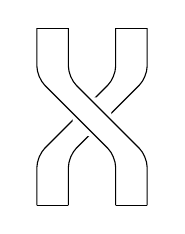
\begin{tikzpicture}[baseline]
				\node(xl1) at (-0.7,1){};
				\node(xr1) at (-0.3,1){};
				\node(yl1) at (0.3,1){};
				\node(yr1) at (0.7,1){};
				\node(yl2) at (-0.7, -1){};
				\node(yr2) at (-0.3, -1){};
				\node(xl2) at (0.3, -1){};
				\node(xr2) at (0.7, -1){};
				\node(b) at (0,0)[circle,fill=white, minimum size=0.5cm]{};
       				\draw[rounded corners](xl1.north) to (-0.7,0.5) to (0.3,-0.5) to (xl2.south);
       				\draw[rounded corners](xr1.north) to (-0.3,0.5) to (0.7,-0.5) to (xr2.south);
				\begin{pgfonlayer}{bg}
				\draw[rounded corners](yl1.north) to (0.3, 0.5) to (-0.7, -0.5) to (yl2.south);
				\draw[rounded corners](yr1.north) to (0.7, 0.5) to (-0.3, -0.5) to (yr2.south);
    				\end{pgfonlayer}
				\draw(xl1.north) to (xr1.north);
				\draw(xl2.south) to (xr2.south);
				\draw(yl1.north) to (yr1.north);
				\draw(yl2.south) to (yr2.south);
			\end{tikzpicture} & \quad \quad \quad \quad \quad \quad \quad &
			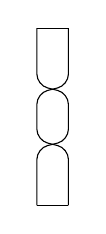
\begin{tikzpicture}[baseline]
				\node(xl1) at (-0.2,1){};
				\node(xr1) at (0.2,1){};	
				\node(xl2) at (-0.2, -1){};
				\node(xr2) at (0.2, -1){};
				\draw[rounded corners](xl1.north) to (-0.2,0.4) to (0.2, 0.3) to (0.2, -0.3) to (-0.2, -0.4) to (xl2.south);	
       				\draw[rounded corners](xr1.north) to (0.2,0.4) to (-0.2, 0.3) to (-0.2, -0.3) to (0.2, -0.4) to (xr2.south);
				\draw(xl1.north) to (xr1.north);
				\draw(xl2.south) to (xr2.south);	
			\end{tikzpicture} \\
			$b$ & & $t$ 
\end{tabular} \end{center}
This operad $RB$\index{action operad!of ribbon braid groups} is also clearly an action operad, since we can just define $\pi^{RB} \colon RB_{n} \rightarrow \Sigma_n$ to act like $\pi^B$ on any braids, at which point the fact that $\pi(t) \in S_1 = \{e_1\}$ will automatically take care of the twists.

\begin{example}
Every abelian group $A$ gives rise to action operad $A^{\bullet}$\nomenclature[N]{$A^{\bullet}$}{action operad of an abelian group $A$}\index{action operad!of an abelian group} as follows.  The group $A^{\bullet}(n)$ is the direct sum of $n$ copies of $A$, $A^{n}$.  The identity element is required to be $e \in A^{1}$, and the multiplication is defined by
  \[
    \mu((a_{1}, \ldots, a_{n}); \mb{b_{1}}, \ldots, \mb{b_{n}}) = (a_{1}+\mb{b_{1}}, a_{2} + \mb{b_{2}}, \ldots, a_{n} + \mb{b_{n}})
  \]
where $\mb{b_{i}}$ is the string $b_{i1}, \ldots, b_{in_{i}}$, and $a_{i} + \mb{b_{i}}$ is
  \[
    a_{i} + b_{i1}, a_{i} + b_{i2}, \ldots, a_{i} + b_{in_{i}}.
  \]
\end{example}


Action operads are themselves the objects of a category, $\mb{AOp}$\nomenclature[C]{$\mb{AOp}$}{of action operads and maps of action operads}.  The morphisms of this category are defined below.
\begin{Defi}\label{mapaop}
A \textit{map of action operads}\index{action operad!maps} $f \colon  \ML \rightarrow \ML'$ consists of a map $f \colon \Lambda \rightarrow \Lambda'$ of the underlying operads such that
  \begin{enumerate}
    \item $\pi^{\Lambda'} \circ f = \pi^{\Lambda}$ (i.e., $f$ is a map of operads over $\Sigma$) and
    \item each $f_{n} \colon \Lambda(n) \rightarrow \Lambda'(n)$ is a group homomorphism.
  \end{enumerate}
\end{Defi}

\begin{Defi}\label{Defi:cat_aop}
The category $\mb{AOp}$\index{action operad!category of} of action operads has objects which are action operads $\mb{\Lambda}$ and
 morphisms $\mb{\Lambda} \rightarrow \mb{\Lambda'}$ as defined in \cref{mapaop}.
\end{Defi}

\section{Some algebra in action operads}
 	QQQ chapter: some algebra in action operads
 	\begin{itemize}
 		\item discusses group-like properties of action operads and their maps: kernels, short exact sequences, fitting Grp-operads into the picture
 		\item some useful technical algebraic lemmas
 		\item algebraic characterisation of action operads via $\beta$ and $\delta$ maps
 	\end{itemize}

We begin with a simple proposition.

\begin{prop}
The map $\pi \colon \ML \rightarrow \mb{\Sigma}$ is a map of action operads.
\end{prop}


\begin{prop}\label{Z}
There is a functor $Z \colon  \mb{Op}(\mb{Grp}) \rightarrow \mb{AOp}$\nomenclature[C]{$\mb{Op}(\mb{Grp})$}{of operads in groups and maps of operads in groups} from the category of operads in groups (using the cartesian monoidal structure) to the category of action operads.  This functor is full, faithful, and its image is precisely the collection of action operads $\ML$ with $\pi_{n}(g) = e_{n}$ for all $n \in \mathbb{N}$, $g \in \Lambda(n)$.
\end{prop}
\begin{proof}
Given an operad in groups $P$, $Z(P)$ is the action operad with the same underlying operad and each $\pi_{n}$ the zero map.  It is easy to verify that $\mu$ is a group homomorphism if and only if $\pi_{n}$ is zero for all $n$, and further that maps between such action operads are precisely the same thing as maps between the corresponding operads in the category of groups.
\end{proof}

We have the following corollary.
\begin{cor}\label{corZ}
For an action operad $\ML$, the sets\index{action operad!kernel}
  \[
    \mathrm{Ker}\,\pi_n = \{g \in \Lambda(n)  \colon  \pi_{n}(g) = e_{n} \}
  \]
form an action operad for which the inclusion $\mathrm{Ker}\,\pi \hookrightarrow \Lambda$ is a map of action operads.
\end{cor}
\begin{proof}
For $\textrm{Ker}\,\pi \hookrightarrow \Lambda$ to be a map of action operads, we must define the map $\textrm{Ker}\,\pi \rightarrow \Sigma$ to be zero,  and we must check that the operadic multiplication of elements in the kernel is also in the kernel.  This last fact is a trivial consequence of $\pi$ being an operad map.
\end{proof}
\begin{cor}\label{image}
For an action operad $\ML$, the sets
  \[
    \mathrm{Im}\pi_n = \{\pi_n(g)~:~g \in \Lambda(n)\}
  \]
form an action operad for which the inclusion $\mathrm{Im}\pi \hookrightarrow \Sigma$ is a map of action operads.
\end{cor}
\begin{proof}
The operad multiplication of elements in the image is also in the image, as is the unit element in $\mathrm{Im}\pi_1$, following again as a consequence of $\pi$ being an operad map. The map $\mathrm{Im}\pi \hookrightarrow \Sigma$ is an inclusion and so is immediately seen to be a map of action operads.
\end{proof}

\begin{prop}[Corollary 2.17,  \cite{zhang-grp}]\label{surjortriv}
The homomorphisms $\pi_n \colon \Lambda_n \rightarrow \Sigma_n$ are either all surjective or all the zero map.
\end{prop}
\begin{proof}
We will prove each case separately. The two cases coincide for $n = 0$ and $n = 1$ as $\pi_0$ and $\pi_1$ are both the zero map and since $\Sigma_0$ and $\Sigma_1$ are the trivial group then these maps are also surjective.

Any homomorphism $G \rightarrow \Sigma_2$ must necessarily be surjective or the zero map. To begin we will show that if $\pi_2 \colon \Lambda(2) \rightarrow \Sigma_2$ is surjective then, by induction, the rest of the maps $\pi_n$ are also surjective. If $\pi_2$ is surjective then there exists an element $g_{1,1} \in \Lambda(2)$ such that $\pi_2(g_{1,1}) = (1 \,\,\, 2)$. Now assume that for some $j \geq 2$ that $\pi_j$ is surjective. In particular, this means that for each transposition $(a \,\,\, a + k) \in \Sigma_j$, where $1 \leq a \leq j-1$ and $a + k \leq j$, there exists $g_{a,k} \in \Lambda(j)$ such that $\pi_j(g_{a,k}) = (a \,\,\, a + k)$. We will use these assumptions to show that each transposition in $\Sigma_{j+1}$ can be written as the image under $\pi_{j+1}$ of some element in $\Lambda(j+1)$, hence any permutation in $\Sigma_{j+1}$ can similarly be written.


Let $(a \,\,\, a +k) \in \Sigma_j$, where $1 \leq a \leq j$ and $a + k \leq j+1$. If $a + k \leq j$, then $(a \,\,\, a + k) = (a \,\,\, a + k)(j + 1) \in \Sigma_{j+1}$. This transposition can be written as
  \begin{align*}
    (a \,\,\, a + k) &= \mu^{\Sigma}(e_2 ; (a \,\,\, a + k), e_1) \\
              &= \mu^{\Sigma}(\pi_2(e_2); \pi_j(g_{a,k}), \pi_1(e_1)) \\
              &= \pi_{j+1}\left(\mu^{\Lambda}(e_2; g_{a,k},e_1)\right).
  \end{align*}
Similarly, if $a > 1$ then this transposition can be written as
  \begin{align*}
    (a \,\,\, a + k) &= \mu^{\Sigma}(e_2 ; e_1, (a-1 \,\,\, a + k-1)) \\
              &= \mu^{\Sigma}(\pi_2(e_2); \pi_1(e_1), \pi_j(g_{a-1,k})) \\
              &= \pi_{j+1}\left(\mu^{\Lambda}(e_2; e_1, g_{a-1,k})\right).
  \end{align*}
Finally, if $a = j$ and $k = 1$, then $(a \,\,\, a + k) = (j \,\,\, j + 1)$. This can be written as
  \begin{align*}
    (j \,\,\, j + 1) &= \mu^{\Sigma}(e_2 ; e_{j-1}, (1 \,\,\, 2)) \\
              &= \mu^{\Sigma}(\pi_2(e_2); \pi_{j-1}(e_{j-1}), \pi_2(g_{1,1})) \\
              &= \pi_{j+1}\left(\mu^{\Lambda}(e_2; e_{j-1}, g_{1,1})\right).
  \end{align*}
Hence $\pi_{j+1}$ is surjective and so all $\pi_n$ are surjective.

Now instead suppose that $\pi_2 \colon \Lambda(2) \rightarrow \Sigma_2$ is the zero map. Assume that $\pi_j \colon \Lambda(j) \rightarrow \Sigma_j$ is the zero map for some $j \geq 2$. Letting $\sigma \in \textrm{Im}\pi_{j+1}$, there exists $g \in \Lambda(j+1)$ such that $\pi_{j+1}(g) = \sigma$. We can then consider the elements $\mu^\Sigma(\sigma; \underline{e_1}, e_o, \underline{e_1})$ where $\underline{e_1}$ means a sequence of $e_1$'s and with $e_0$ in the $k$th position, with $1 \leq k \leq j + 1$. Now
  \begin{align*}
    \mu^\Sigma(\sigma; \underline{e_1}, e_o, \underline{e_1}) &= \mu^\Sigma(\pi_{j+1}(g); \underline{\pi_1(e_1)}, \pi_0(e_0), \underline{\pi_1(e_1)}) \\
    &= \pi_j(\mu^\Lambda(g; \underline{e_1}, e_0, \underline{e_1})) \\
    &= e_j.
  \end{align*}
We can think of this permutation as being $\sigma$ with the $k$th string removed. Now each of these is the identity $e_j$, as shown above. This means that $\sigma$ must either have been the identity $e_{j+1}$ or a transposition of the form $(a \,\,\, a + 1)$, where $1 \leq a \leq j$.

If $\sigma$ is the identity $e_{j+1}$, then we are done since this would give $\textrm{Im}\pi_{j+1} = \{e_{j+1}\}$. Instead suppose that $\sigma = (a \,\,\, a + 1) \in \Sigma_{j + 1}$. Then if $1 < a \leq j$ we can use this to give
  \begin{align*}
    (a -1 \,\,\, a) &= \mu^\Sigma((a \,\,\, a + 1); e_0, \underline{e_1}) \\
    &= \mu^\Sigma(\pi_{j+1}(g);\pi_0(e_0), \underline{\pi_1(e_1)}) \\
    &= \pi_j(\mu^\Lambda(g; e_0, \underline{e_1})) \\
    &= e_j.
  \end{align*}
This gives a contradiction, hence $\sigma \neq (a \,\,\, a + 1)$ and must be the identity $e_{j+1}$.

Similarly, if $\sigma = (1 \,\,\, 2) \in \Sigma_{j+1}$, then in $\Sigma_j$ we find that
  \begin{align*}
    (1 \,\,\, 2) &= \mu^\Sigma((1 \,\,\, 2) ; \underline{e_1}, e_0) \\
    &= \mu^\Sigma(\pi_{j+1}(g); \underline{\pi_1(e_1)}, \pi_0(e_0)) \\
    &= \pi_j(\mu^\Lambda(g ; \underline{e_1}, e_0)) \\
    &= e_j.
  \end{align*}
Again, a contradiction, hence $\sigma = e_{j+1}$.
\end{proof}

\begin{cor}\label{extension}
Every action operad $\ML$ with nontrivial $\pi$ fits into a short exact sequence
  \[
    T \rightarrow \textrm{Ker}\,\pi \hookrightarrow \Lambda \stackrel{\pi}{\longrightarrow} \Sigma \rightarrow T,
  \]
by which we mean this is a sequence of action operad maps which is an exact sequence of groups at each $n$.
\end{cor}

\begin{rem}
Thus we see that an action operad is either an operad in groups, or is an extension of $\Sigma$ by an operad in groups. This gives a simple proof that the operads of pure braids and pure ribbon braids are both operads in groups.
\end{rem}

\begin{rem}
The crossed simplicial groups\index{crossed simplicial group} of Fiedoriwicz and Loday \cite{FL91} are related to action operads in the following way. There is a functor $C \colon \mathbf{AOp} \rightarrow \mathbf{CSGrp}$\nomenclature[C]{$\mathbf{CSGrp}$}{of crossed simplicial groups and morphisms of crossed simplicial groups} from the category of action operads just described into the category of crossed simplicial groups. This functor takes an action operad $\ML$ and defines $C(\Lambda)(n) = \Lambda_{n+1}$. The face and degeneracy maps of the underlying simplicial structure are defined using the operadic composition inherent to $\Lambda$ - the description of the maps via the operad structure can be viewed in a similar way to Construction 1.1 of \cite{Kra96}. This functor is, however, not faithful, nor is it conservative. (Recall that a functor $F \colon \mathcal{C} \rightarrow \mathcal{D}$ is conservative if when $Ff$ is an isomorphism in $\mathcal{D}$, then $f$ is an isomorphism in $\mathcal{C}$.)
\end{rem}
%Salvatore-Wahl:  Framed disks operads\ldots

We now study some of the structure on the groups $\Lambda(n)$ for small values of $n$. Recall that $e_{n}$ is the identity element in the group $\Lambda(n)$.

\begin{lem}\label{G0abel}
Let $\ML$ be an action operad. The group $\Lambda(0)$ is abelian, and its group operation coincides with the operation 
  \[
    g, h \in \Lambda(0) \mapsto \mu(e_2; g, h)
  \]
arising from the operad structure.
\end{lem}
\begin{proof}
\end{proof}

\begin{lem}\label{calclem}
Let $\ML$ be an action operad.
\begin{enumerate}
\item In $\Lambda(1)$, the unit element $e_{1}$ for the group structure is equal to the identity element for the operad structure, $\id$.
\item The equation
  \[
    \mu(e_{n}; e_{i_{1}}, \ldots, e_{i_{n}}) = e_{I}
  \]
holds for any natural numbers $n, i_{j}, I = \sum i_{j}$.
\item The group $\Lambda(1)$ is abelian.
\end{enumerate}
\end{lem}
\begin{proof}
For the first claim, let $g \in \Lambda(1)$.  Then
  \begin{align*}
    g & = g \cdot e_{1} \\
    &= \mu(g; \id) \cdot \mu(\id; e_{1}) \\
    &= \mu(g \cdot \id; \id \cdot e_{1}) \\
    &= \mu(g \cdot \id; \id) \\
    &= g \cdot \id
  \end{align*}
using that $e_{1}$ is the unit element for the group structure, that $\id$ is a two-sided unit for operad multiplication, and the final axiom for an action operad together with the fact that the only element of the symmetric group $\Sigma_{1}$ is the identity permutation.  Thus $g = g \cdot \id$, so $\id = e_{1}$.

For the second claim, write the operadic product as $\mu(e; \underline{e})$, and consider the square of this element. We have
  \begin{align*}
    \mu(e; \underline{e}) \cdot \mu(e; \underline{e}) & = \mu(e \cdot e; \underline{e} \cdot \underline{e}) \\
    &= \mu(e; \underline{e})
  \end{align*}
where the first equality follows from the last action operad axiom together with the fact that $e$ gets mapped to the identity permutation; here $\underline{e} \cdot \underline{e}$ is the sequence $e_{i_{1}} \cdot e_{i_{1}}, \ldots, e_{i_{n}} \cdot e_{i_{n}}$.  Thus $\mu(e; \underline{e})$ is an idempotent element of the group $\Lambda(I)$, so must be the identity element $e_{I}$.

For the final claim, note that the specific operadic multiplication map $\mu \colon \Lambda(1) \times \Lambda(1) \rightarrow \Lambda(1)$ is a group homomorphism following from the action operad axioms, and $\id = e_{1}$ is a two-sided unit, so the Eckmann-Hilton argument shows that $\mu$ is actually group multiplication and that $\Lambda_{1}$ is abelian.
\end{proof}

Note that the operad of symmetric groups $\Sigma$ has its action operad structure determined by two auxiliary operations.  The first is the block sum of permutations which we denote by
  \[
    \beta \colon \Sigma_{k_{1}} \times \cdots \times \Sigma_{k_{n}} \rightarrow \Sigma_{K},
  \]
where $K = \sum k_{i}$.  The second is a kind of diagonal map which is defined for any natural number $n$ together with natural numbers $k_{1}, \ldots, k_{n}$.  Then
  \[
    \delta = \delta_{n; k_{1}, \ldots, k_{n}} \colon \Sigma_{n} \rightarrow \Sigma_{\underline{k}},
  \]
is defined on $\sigma \in \Sigma_{n}$ by permuting the elements $1, 2, \ldots, k_{1}$ together in a block according to the action of $\sigma \in \Sigma_{n}$ on $1$, then $k_{1}+1, \ldots, k_{1}+k_{2}$ together in a block according to the action of $\sigma$ on $2$, and so on.  The first of these, $\beta$\nomenclature[N]{$\beta$}{block sum of permutations}, is a group homomorphism, while $\delta$\nomenclature[N]{$\delta$}{diagonal map permuting in a block}
% QQQ Need to run the index command so these appear.
is a sort of twisted homomorphism, and taken together they define operadic multiplication in $\Sigma$.  We now use these ideas to give the following algebraic characterization of action operads via the following definition.

\begin{Defi}\label{Defi:aop_bl}
Let $\ML$ be an action operad. For $h_i \in \Lambda(k_i)$ and $g \in \Lambda(n)$, define
  \begin{align*}
    \beta(h_{1}, \ldots, h_{n}) &= \mu(e; h_{1}, \ldots, h_{n}), \\
    \delta_{n; k_{1}, \ldots, k_{n}}(g) &= \mu(g; e_{k_1}, \ldots, e_{k_n}).
  \end{align*}
\end{Defi}


\begin{thm}\label{thm:charAOp}
An action operad $\mb{\Lambda}$ determines, and is determined by, the following: 
\begin{itemize}
\item groups $\Lambda(n)$ together with group homomorphisms $\pi_{n} \colon \Lambda(n) \rightarrow \Sigma_{n}$,
\item a group homomorphism
  \[
    \Lambda(k_{1}) \times \cdots \times \Lambda(k_{n}) \stackrel{\beta}{\longrightarrow} \Lambda(k_{1} + \cdots + k_{n}),
  \]
for each $k_{1}, \ldots, k_{n}$ together with the degenerate case of $n=0$ which then is a group homomorphism $1 \rightarrow \Lambda(0)$, and
\item a function of sets
  \[
    \Lambda(n) \stackrel{\delta_{n; k_{1}, \ldots, k_{n}}}{\longrightarrow} \Lambda(k_{1} + \cdots + k_{n})
  \]
for each $n, k_{1}, \ldots, k_{n}$,
\end{itemize}
subject to the axioms below.  In what we write below, we use the following notational conventions.
\begin{itemize}
\item The symbols $f,g,h$, with or without subscripts, always refer to an element of some group $\Lambda(n)$.
\item The symbols $j,k,m,n,p$ are all natural numbers, and $i$ is a natural number between 1 and $n$.
\end{itemize}
Axioms:
\begin{enumerate}
\item\label{eq1} The homomorphisms $\beta$ are natural with respect to the maps $\pi_{n}$, where $\underline{k} = k_{1} + \cdots + k_{n}$.
  \[
    \xy
      (0,0)*+{\Lambda(k_{1}) \times \cdots \times \Lambda(k_{n}) } ="00";
      (0,-15)*+{\Sigma_{k_{1}} \times \cdots \times \Sigma_{k_{n}}  } ="01";
      (40,0)*+{\Lambda(\underline{k}) } ="20";
      (40,-15)*+{\Sigma_{\underline{k}} } ="21";
      {\ar^{\beta} "00" ; "20"};
      {\ar^{\pi} "20" ; "21"};
      {\ar_{\pi_1 \times \cdots \times \pi_n} "00" ; "01"};
      {\ar_{\beta} "01" ; "21"};
    \endxy
  \]
\item\label{eq2} The homomorphism $\beta \colon \Lambda(k) \rightarrow \Lambda(k)$ is the identity.
\item\label{eq3} The homomorphisms $\beta$ are associative in the sense that the equation
% \[
% \beta(h_{11}, \ldots, h_{1j_{1}}, h_{21}, \ldots, h_{2j_{2}}, \ldots, h_{nj_{n}}) = \beta\left( \beta(h_{11}, \ldots, h_{1j_{1}}), \ldots, \beta(h_{n1}, \ldots, h_{nj_{n}}) \right)
% \]
\[
  \beta(\underline{h_1},\ldots,\underline{h_n}) = \beta(\beta(\underline{h_1},\ldots,\beta(\underline{h_n}))
\]
holds, where $\underline{h_i} = h_{i1},\ldots,h_{ij_i}$.
\item\label{eq4} The functions $\delta_{n; k_{1}, \ldots, k_{n}}$ are natural with respect to the maps $\pi_{n}$.
  \[
    \xy
      (0,0)*+{\Lambda(n)} ="00";
      (40,0)*+{\Lambda(k_{1} + \cdots + k_{n}) } ="20";
      (0,-15)*+{\Sigma_{n}  } ="01";
      (40,-15)*+{\Sigma_{k_{1} + \cdots + k_{n}} } ="21";
      {\ar^{\delta} "00" ; "20"};
      {\ar^{\pi} "20" ; "21"};
      {\ar_{\pi} "00" ; "01"};
      {\ar_{\delta} "01" ; "21"};
    \endxy
  \]
\item\label{eq5} The functions $\delta_{n; 1, \ldots, 1}, \, \delta_{1;n} \colon \Lambda(n) \rightarrow \Lambda(n)$ are the identity.
\item\label{eq6} The equation $\delta_{n; k_{i}}(g) \delta_{n; j_{i}}(h) = \delta_{n; j_{i}}(gh)$ holds when
  \[
    k_{i} = j_{\pi(h)^{-1}(i)}.
  \]
\item\label{eq7} The functions $\delta$ are associative in the sense that the equation
% \[
% \delta_{m_1 + \cdots + m_n; p_{11}, \ldots, p_{1m_{1}}, p_{21}, \ldots, p_{nm_{n}}}\left( \delta_{n; m_{1}, \ldots, m_{n}}(f) \right) = \delta_{n; P_{1}, \ldots, P_{n}}(f)
% \]
  \[
    \delta_{m_1 + \cdots + m_n; \underline{p_1},\ldots,\underline{p_n}}\left( \delta_{n; m_{1}, \ldots, m_{n}}(f) \right) = \delta_{n; P_{1}, \ldots, P_{n}}(f)
  \]
holds, where $P_{i} = p_{i1} + \cdots + p_{im_{i}}$ and $\underline{p_i} = p_{i1}, \ldots, p_{im_i}$.
\item\label{eq8} The equation
  \[
    \delta(g) \beta(h_{1}, \ldots, h_{n}) = \beta(h_{\pi(g)^{-1}(1)}, \ldots,  h_{\pi(g)^{-1}(n)}) \delta(g)
  \]
holds, where $h_{i} \in \Lambda(k_{i})$ and $\delta \colon \Lambda(n) \rightarrow \Lambda(k_{1} + \cdots + k_{n})$.
\item\label{eq9} The equation
  \[
    \beta(\delta_{1}(g_{1}), \ldots, \delta_{n}(g_{n})) = \delta_{c}(\beta(g_{1}, \ldots, g_{n}))
  \]
holds, where $\delta_{i}(g_{i})$ is shorthand for $\delta_{k_{i}; m_{i1}, \ldots, m_{ik_{i}}}(g_{i})$ and $\delta_{c}$ is shorthand for
  \[
    \delta_{k_{1}+\cdots + k_{n}; m_{11}, m_{12}, \ldots, m_{1k_{1}}, m_{21}, \ldots, m_{nk_{n}}}.
  \]
\end{enumerate}
\end{thm}

\begin{proof}
Let $\mb{\Lambda}$ be an action operad, and define $\beta, \delta$ as in \cref{Defi:aop_bl}.  Since $\pi \colon \Lambda \rightarrow \Sigma$ is an operad map, axioms \eqref{eq1} and \eqref{eq4} hold.  Since $\Lambda$ is an operad of sets, axioms \eqref{eq2} and \eqref{eq5} follow from the operad unit axioms, and axioms \eqref{eq3}, \eqref{eq7}, and \eqref{eq9} follow from the operad associativity axiom.  Axioms \eqref{eq6} and \eqref{eq8} are special cases of the additional action operad axiom, as is the fact that $\beta$ is a group homomorphism.

Conversely, given the data above, we need only define the operad multiplication, verify the operad unit and multiplication axioms,  and finally check the action operad axiom.  Multiplication is given by
  \[
    \mu(g; h_{1}, \ldots, h_{n}) = \delta_{n; k_{1}, \ldots, k_{n}}(g) \beta(h_{1}, \ldots, h_{n})
  \]
where $h_{i} \in \Lambda(k_{i})$.  The unit is $e \in \Lambda(1)$.

We now verify the operad unit axioms.
  \begin{align*}
    \mu(e; g) &= \delta(e)\beta(g) \\
    &= e \cdot g \\
    &= g \\
    \mu(h; e, \ldots, e) &= \delta(h)\beta(e, \ldots, e) \\
    &= h \cdot e \\
    &= h
  \end{align*}
These follow from axioms \eqref{eq2} and \eqref{eq5}, together with the fact that $\beta$ is a group homomorphism.

For the operad associativity axiom, let
\begin{itemize}
\item $f \in \Lambda(m),$
\item $g_{i} \in \Lambda(n_{i})$ for $i=1, \ldots, m$, and
\item $h_{ij} \in \Lambda(p_{i,j})$ for $i=1, \ldots, m$ and $j=1, \ldots, n_{i}$.
\end{itemize}
Further, let $P_{i} = p_{i1} + \cdots + p_{in_{i}}$ and $\underline{h_i}$ denote the list $h_{i1}, h_{i2}, \ldots, h_{in_{i}}$.  We must then show that
  \[
    \mu\left( f; \mu\left(g_{1}; \underline{h_1}\right), \ldots, \mu\left(g_{m}; \underline{h_m}\right) \right) = \mu\left( \mu\left(f; g_{1}, \ldots, g_{m}\right); \underline{h_1}, \ldots, \underline{h_m} \right).
  \]
By definition, the left side of this equation is
  \[
    \delta_{m; P_{1}, \ldots, P_{m}}(f) \beta\left( \mu\left(g_{1}; \underline{h_1}\right), \ldots, \mu\left(g_{m}; \underline{h_m}\right) \right),
  \]
and
  \[
    \mu\left(g_{i}; \underline{h_i}\right) = \delta_{n_{i}; p_{i1}, \ldots, p_{in_{i}}}(g_{i})\beta\left(h_{i1}, \ldots, h_{in_{i}}\right).
  \]
Since $\beta$ is a group homomorphism, we can then rewrite the left side as
  \[
    \delta(f)\beta\left(\delta(g_{1}), \ldots, \delta(g_{m})\right)\beta\left(\beta\left(\underline{h_1}\right), \ldots, \beta\left(\underline{h_m}\right)\right)
  \]
where we have suppressed the subscripts on the $\delta$'s.  By axiom \eqref{eq3} , we have
  \[
    \beta\left(\beta\left(\underline{h_1}\right), \ldots, \beta\left(\underline{h_m}\right)\right) = \beta\left(\underline{h_1},\ldots,\underline{h_m}\right).
  \]
Further, axiom \eqref{eq9} above shows that
  \[
    \beta\left(\delta(g_{1}), \ldots, \delta\left(g_{m}\right)\right) = \delta\left(\beta\left(g_{1}, \ldots, g_{m}\right)\right).
  \]
Thus we have shown that the left side of the operad associativity axiom is equal to
  \[
    \delta(f)\delta\left(\beta(g_{1}, \ldots, g_{m})\right)\beta\left(\underline{h_1},\ldots,\underline{h_m}\right).
  \]
Now the right side is
  \[
    \mu\left( \mu (f; g_{1}, \ldots, g_{m}); \underline{h_1}, \ldots, \underline{h_m} \right)
  \]
which is by definition
  \[
    \delta\left(\mu (f; g_{1}, \ldots, g_{m})\right)\beta\left(\underline{h_1}, \ldots, \underline{h_m}\right).
  \]
Thus verifying the operad associativity axiom reduces to showing
\begin{eqn}\label{eqn:opass}
\delta(f)\delta\left(\beta(g_{1}, \ldots, g_{m})\right) = \delta\left(\mu (f; g_{1}, \ldots, g_{m})\right).
\end{eqn}By the definition of $\mu$, we have
  \[
    \delta(\mu (f; g_{1}, \ldots, g_{m})) = \delta\left(\delta(f)\beta(g_{1}, \ldots, g_{m}) \right)
  \]
which is itself equal to
\begin{eqn}\label{eqn:opass2}
\delta\left(\delta(f)\right) \delta\left(\beta(g_{1}, \ldots, g_{m})\right)
\end{eqn}by axiom \eqref{eq6} above.  Now the $\delta(f)$ on the left side of \cref{eqn:opass} uses $\delta_{n; P_{1}, \ldots, P_{n}}$, while the $\delta(\delta(f))$ in \cref{eqn:opass2} is actually
  \[
    \delta_{m_1 + \cdots + m_{n}; q_{ij}}(\delta_{n; m_{1}, \ldots, m_{n}} (f))
  \]
where the $q_{ij}$ are defined, by axiom \eqref{eq6}, to be given by
  \[
    q_{ij} = p_{i,\pi(g_{i})^{-1}(j)}
  \]
using the compatibility of $\beta$ and $\pi$ in axiom \eqref{eq1}.  By axiom \eqref{eq7}, this composite of $\delta$'s  is then $\delta_{n; Q_{1}, \ldots, Q_{n}}$ where $Q_{i} = q_{i1} + \cdots + q_{im_{i}}$.  But by the definition of the $q_{ij}$, we immediately see that $Q_{i} = P_{i}$, so the $\delta(f)$ in \cref{eqn:opass} is equal to the $\delta(\delta(f))$ appearing in \cref{eqn:opass2}, concluding the proof of the operad associativity axiom.

The action operad axiom is now the calculation below, and uses axioms \eqref{eq4} and \eqref{eq8}.
\begin{small}
  \begin{align*}
    \mu\left(g; h_{1}, \ldots, h_{n}\right)\mu\left(g'; h_{1}', \ldots, h_{n}'\right) &= \delta\left(g\right) \beta\left(h_{1}, \ldots, h_{n}\right) \delta\left(g'\right) \beta\left(h_{1}', \ldots, h_{n}'\right) \\
    &= \delta\left(g\right) \delta\left(g'\right) \beta\left(h_{\pi\left(g'\right)(1)}, \ldots, h_{\pi\left(g'\right)(n)}\right)  \beta\left(h_{1}', \ldots, h_{n}'\right) \\
    &= \delta\left(gg'\right) \beta\left(h_{\pi\left(g'\right)(1)}h_{1}', \ldots, h_{\pi\left(g'\right)(n)}h_{n}'\right) \\
    &= \mu\left(gg'; h_{\pi\left(g'\right)(1)}h_{1}', \ldots, h_{\pi\left(g'\right)(n)}h_{n}'\right)
  \end{align*}
\end{small}
\end{proof}

\begin{nota}\label{beta_to_oplus}
Leaning more heavily into the interpretation that the operations denoted $\beta$ above are block sums, we also write $g_1 \oplus g_2 \oplus \cdots \oplus g_n$ for
$\beta(g_1, g_2, \ldots, g_n)$.
\end{nota}

\section{Presentations of action operads}\label{sec:presofacops}
A useful method for constructing new examples of some given algebraic structure is through the use of presentations. A presentation consists of generating data together with relations between generators using the operations of the algebra involved.  In categorical terms, the generators and relations are both given as free gadgets on some underlying data, and the presentation itself is a coequalizer. This section will establish the categorical structure necessary to give presentations for action operads, and then explain how such a presentation is reflected in the associated club and 2-monad. The most direct route to the desired results uses the theory of locally finitely presentable categories. We recall the main definitions briefly, but refer the reader to \cite{ar} for additional details.

\begin{Defi}\label{def:filtered}
  A \textit{filtered category}\index{category!filtered} is a nonempty category $C$ such that
    \begin{itemize}
      \item if $a,b$ are objects of $C$, then there is another object $c \in C$ and morphisms $a \rightarrow c, b \rightarrow c$; and
      \item if $f,g \colon a \rightarrow b$ are parallel morphisms in $C$, then there exists a morphism $h \colon b \rightarrow c$ such that $hf = hg$.
    \end{itemize}
\end{Defi}

\begin{Defi}
  A \emph{filtered colimit}\index{colimit!filtered} is a colimit over a filtered category.
\end{Defi}

\begin{Defi}
  Let $C$ be a category with all filtered colimits.  An object $x \in C$ is \textit{finitely presentable}\index{object!finitely presentable} if the representable functor $C(x, -) \colon C \rightarrow \mb{Sets}$ preserves filtered colimits.
\end{Defi}

\begin{Defi}
  A \textit{locally finitely presentable category}\index{category!locally finitely presentable} is a category $C$ such that
  \begin{itemize}
    \item $C$ is cocomplete and
    \item there exists a small subcategory $C_{fp}\nomenclature[C]{$C_{fp}$}{the subcategory of finitely presentable objects in $C$} \subseteq C$ of finitely presentable objects such that any object $x \in C$ is the filtered colimit of some diagram in $C_{fp}$.
  \end{itemize}
\end{Defi}

The definition of a locally finitely presentable category has many equivalent variants, and our applications are quite straightforward so we have given a commonly stated version of the definition.


\begin{thm}
The category $\mb{AOp}$ is locally finitely presentable.
\end{thm}
\begin{proof}
First note that there is a category $\mb{Op}^{g}$\nomenclature[C]{$\mb{Op}^{g}$}{of operads $P$ for which each $P(n)$ has a group structure and operad maps}, whose objects are operads $P$ in which each $P(n)$ also carries a group structure. This is an equational theory using equations with only finitely many elements, so $\mb{Op}^{g}$ is locally finitely presentable \cite[Corollary 3.7]{ar}. A slice category of a locally finitely presentable category is itself locally finite presentable \cite[Proposition 1.57]{ar} and since the symmetric operad is an object of $\mb{Op}^{g}$, the slice category\index{category!slice category} $\mb{Op}^{g}/\Sigma$ is locally finitely presentable.

There is an obvious inclusion functor $\mb{AOp} \hookrightarrow \mb{Op}^{g}/\Sigma$.  Now $\mb{AOp}$ is a full subcategory of $\mb{Op}^{g}/\Sigma$ which is closed under products, subobjects. Since any object of $\mb{Op}^{g}/\Sigma$ isomorphic to an action operad is in fact an action operad, the inclusion   $\mb{AOp} \hookrightarrow \mb{Op}^{g}/\Sigma$ is actually the inclusion of a reflective subcategory.  One easily checks that $\mb{AOp}$ is in fact closed under all limits and filtered colimits in $\mb{Op}^{g}/\Sigma$, so by the Reflection Theorem (2.48 in \cite{ar}), $\mb{AOp}$ is locally finitely presentable.
\end{proof}

\begin{Defi}
  Let $\SS$ be the set which is the disjoint union of the underlying sets of all the symmetric groups.  Then $\mb{Sets}/\SS$ is the slice category over $\SS$ with objects $(X,f)$ where $X$ is a set and $f \colon X \rightarrow \SS$ and morphisms $(X_{1}, f_{1}) \rightarrow (X_{2}, f_{2})$ are those functions $g \colon X_{1} \rightarrow X_{2}$ such that $f_{1} = f_{2}g$.  We call an object $(X,f)$ a \textit{collection over $\SS$}.
\end{Defi}

\begin{rem}
In standard presentations of the theory of operads (see, for example, \cite{mss-op}), a nonsymmetric operad will have an underlying collection\index{collection!non-symmetric} (or $\mathbb{N}$-indexed collection of sets) while a symmetric operad will have an underlying symmetric collection\index{collection!symmetric} (or $\mathbb{N}$-indexed collection of sets in which the $n$th set has an action of $\Sigma_{n}$).  Our collections over $\SS$ more closely resemble the former as there is no group action present.
\end{rem}

\begin{example}
One can easily form new action operads from old ones by taking limits\index{action operad!limits of}.  To take a limit of a diagram in $\mb{AOp}$, one forgets down to the category of operads over $\Sigma$ and takes the limit there.  Concretely, products in $\mb{AOp}$ are computed as products in $\mb{Op}/\Sigma$\nomenclature[C]{$C/c$}{the slice category of $C$ over an object $c$ in $C$} (see QQQ) which themselves are (possibly wide) pullbacks in the category of operads.  This pullback will then be computed levelwise, showing that at each dimension we have a group structure with a group homomorphism to the appropriate $\Sigma_{n}$ and that the final action operad axiom holds since it does in each component.  The equalizer of a pair of maps will then just be the levelwise equalizer.  This shows that the pointwise product of an action operad $P$ with an action operad of the form $Z(Q)$ (as in Proposition \ref{Z}) is again an action operad, but the pointwise product of two arbitrary action operads might not be.
\end{example}
\begin{thm}\label{underlyingSS}
There is a forgetful functor $U \colon \mb{AOp} \rightarrow \mb{Sets}/\SS$ which preserves all limits and filtered colimits.
\end{thm}

\begin{proof}
The functor $U$ is obvious, and the preservation of filtered colimits follows from the fact that these are computed pointwise, together with the fact that every map between action operads preserves underlying permutations.
As equalizers are computed levelwise, and the product $\mb{\Lambda} \times \mb{\Lambda}'$ has underlying operad the pullback $\Lambda \times_{\Sigma} \Lambda'$; this pullback is itself computed levelwise.  Together, these imply that $U$ also preserves all limits.
\end{proof}

\begin{cor}
$U$ has a left adjoint $F \colon \mb{Sets}/\SS \rightarrow \mb{AOp}$, the free action operad functor.
\end{cor}
\begin{proof}
The category $\mb{Sets}/\SS$ is locally finitely presentable as it is equivalent to the functor category $[\SS, \mb{Sets}]$\nomenclature[C]{$[A,B]$}{of functors between categories $A$ and $B$ and natural transformations} (here $\SS$ is treated as a discrete category) and any presheaf category is locally finitely presentable.  The functor $U$ preserves limits and filtered colimits between locally finitely presentable categories, so has a left adjoint (see Theorem 1.66 in \cite{ar}).
\end{proof}

\begin{Defi}
  A \textit{presentation}\index{action operad!presentation} for an action operad $\mb{\Lambda}$ consists of
  \begin{itemize}
    \item a pair of collections over $\SS$ denoted $\mathbf{g}, \mathbf{r}$,
    \item a pair of maps $s_{1}, s_{2} \colon F\mathbf{r} \rightarrow F\mathbf{g}$ between the associated free action operads, and
    \item a map $p \colon F\mathbf{g} \rightarrow \mb{\Lambda}$ of action operads exhibiting $\mb{\Lambda}$ as the coequalizer of $s_{1},s_{2}$.
  \end{itemize}
\end{Defi}









\section{Operads and algebras with general group actions}
 	QQQ chapter: operads and algebras with general group actions
 	\begin{itemize}
 		\item defines $\ML$-operads
 		\item goes over familiar examples
 		\item recasts familar operad algebra stuff for $\ML$-operads
 		\begin{itemize}
	 		\item defines algebras and pseudoalgebras for $\ML$-operads
	 		\item characterises algebras using the endomorphism operads
	 		\item monads via operads
	 	\end{itemize}
	 	\item theorem about the adjunction between $\ML-\bf{Op}$ and $\bf{\Sigma}-\bf{Op}$
	 	\item technical results about monad maps
 	\end{itemize}
Just as we had the definitions of operad, symmetric operad, and braided operad, we now come to the general definition of a $\ML$-operad, where $\ML$ is an action operad.

\begin{Defi}\label{Defi:lamop}
  Let $\ML$ be an action operad.  A \textit{$\ML$-operad}\index{operad!$\ML$-operad} $P$ (in $\mb{Sets}$) consists of
    \begin{itemize}
      \item a non-symmetric operad $P$ in $\mb{Sets}$ and
      \item for each $n$, an action $P(n) \times \Lambda(n) \rightarrow P(n)$ of $\Lambda(n)$ on $P(n)$
    \end{itemize}
such that the following two equivariance axioms hold.
  \begin{align*}
    \mu^{P}(x; y_{1} \cdot g_{1}, \ldots, y_{n} \cdot g_{n}) &= \mu^{P}(x; y_{1}, \ldots, y_{n}) \cdot \mu^{\Lambda}(e; g_{1}, \ldots, g_{n})  \\
    \mu^{P}(x \cdot g; y_{1}, \ldots, y_{n}) &= \mu^{P}\left((x; y_{\pi(g)^{-1}(1)}, \ldots, y_{\pi(g)^{-1}(n)}\right) \cdot \mu^{\Lambda}(g; e_{1}, \ldots, e_{n})
  \end{align*}
\end{Defi}

\begin{Defi}
  The category $\ML\mbox{-}\mb{Op}$\nomenclature[C]{$\ML\mbox{-}\mb{Op}$}{of $\ML$-operads and maps of operads which are levelwise equivariant with respect to the $\Lambda(n)$-actions}\index{operad!$\ML$-operad!category of} of $\Lambda$-operads has objects the $\ML$-operads and morphisms those maps of operads which are levelwise equivariant with respect to the $\Lambda(n)$-actions.
\end{Defi}

\begin{example}
  \begin{enumerate}
    \item Let $\mb{T}$\index{action operad!initial}\index{operad!terminal} denote the terminal operad in $\mb{Sets}$ equipped with its unique action operad structure.  Then a $\mb{T}$-operad is just a non-symmetric operad in $\mb{Sets}$.
    \item Let $\mb{\Sigma}$\index{operad!of symmetric groups} denote the operad of symmetric groups with $\pi \colon \Sigma \rightarrow \Sigma$ the identity map.  Then a $\mb{\Sigma}$-operad is a symmetric operad in the category of sets.
    \item Let $\mb{B}$\index{operad!of braid groups} denote the operad of braid groups with $\pi_{n} \colon B_{n} \rightarrow \Sigma_{n}$ the canonical projection of a braid onto its underlying permutation.  Then a $\mb{B}$-operad is a braided operad in the sense of Fiedorowicz \cite{fie-br}.
  \end{enumerate}
\end{example}

A further example of a $\ML$-operad is given by the underlying operad, $\Lambda$, of $\ML$ itself.
\begin{prop}\label{gisgop}
Let $\mb{\Lambda}$ be an action operad.  Then the operad $\Lambda$ is itself a $\mb{\Lambda}$-operad.
\end{prop}
\begin{proof}
The underlying operad $\Lambda$ is of course an operad in $\mb{Sets}$. The action $\Lambda(n) \times \Lambda(n) \rightarrow \Lambda(n)$ is given simply by the group multiplication in $\Lambda(n)$. The two equivariance axioms are then both instances of the action operad axiom of $\ML$.
\end{proof}

An operad is intended to be an abstract description of a certain type of algebraic structure, and the particular instances of that structure are the algebras for that operad.  We begin with the definition of an algebra over a non-symmetric operad and add in the group actions later.

\begin{Defi}\label{opalgax}
Let $O$ be a non-symmetric operad.  An \textit{algebra}\index{algebra!operad}\index{operad!algebra} for $O$ consists of a set $X$ together with maps $\alpha_{n} \colon O(n) \times X^{n} \rightarrow X$ such that the following axioms hold.
\begin{enumerate}
\item The element $\id \in O(1)$ is a unit in the sense that
  \[
    \alpha_{1}(\id; x) = x
  \]
for all $x \in X$.
\item The maps $\alpha_{n}$ are associative in the sense that the following diagram commutes.
  \[
    \xy
      (0,0)*+{O(n) \times O(k_{1}) \times X^{k_{1}} \times \cdots \times O(k_{n}) \times X^{k_{n}}}="ul";
      (75,0)*+{O(n) \times X^{n}}="ur";
      (0,-12)*+{O(n) \times O(k_{1}) \times \cdots \times O(k_{n}) \times X^{k_{1}} \times \cdots \times X^{k_{n}}}="ml";
      (0,-24)*+{O(\sum k_{i}) \times X^{\sum k_{i}}}="bl";
      (75,-24)*+{X}="br";
      {\ar^>>>>>>>>>>>>>>{1 \times \alpha_{k_{1}} \times \cdots \alpha_{k_{n}}} "ul"; "ur"};
      {\ar^{\alpha_{n}} "ur"; "br"};
      {\ar_{\cong} "ul"; "ml"};
      {\ar_{\mu \times 1} "ml"; "bl"};
      {\ar_{\alpha_{\sum k_{i}}} "bl"; "br"};
    \endxy
  \]
\end{enumerate}
\end{Defi}


Moving on to algebras for a $\ML$-operad, let $P$ be a $\ML$-operad and let $X$ be any set.  Write $P(n) \times_{\Lambda(n)} X^{n}$ for the coequalizer of the pair of maps
  \[
    P(n) \times \Lambda(n) \times X^{n} \rightrightarrows P(n) \times X^{n}
  \]
of which the first map is the action of $\Lambda(n)$ on $P(n)$ and the second map is
  \[
    P(n) \times \Lambda(n) \times X^{n} \rightarrow P(n) \times \Sigma_{n} \times X^{n} \rightarrow P(n) \times X^{n}
  \]
using $\pi_{n} \colon \Lambda(n) \rightarrow \Sigma_{n}$ together with the canonical action of $\Sigma_{n}$ on $X^{n}$ by permutation of coordinates: $\sigma \cdot (x_{1}, \ldots, x_{n}) = (x_{\sigma^{-1}(1)}, \ldots, x_{\sigma^{-1}(n)})$.  By the universal property of the coequalizer, a function $f \colon P(n) \times_{\Lambda(n)} X^{n} \rightarrow Y$ can be identified with a function $\tilde{f} \colon P(n) \times X^{n} \rightarrow Y$ such that
  \[
    \tilde{f}(p\cdot g; x_{1}, \ldots, x_{n}) = \tilde{f}\left(p; x_{\pi(g)^{-1}(1)}, \ldots, x_{\pi(g)^{-1}(n)}\right).
  \]

\begin{Defi}
  Let $P$ be a $\ML$-operad.  An \textit{algebra}\index{algebra!$\Lambda$-operad} for $P$ consists of a set $X$ together with maps $\alpha_{n} \colon P(n) \times_{\Lambda(n)} X^{n} \rightarrow X$ such that the maps $\tilde{\alpha}_{n}$ satisfy the operad algebra axioms given in Definition \ref{opalgax}.
\end{Defi}

\begin{rem}
It is worth noting that the equivariance required for a $P$-algebra is built into the definition above by requiring the existence of the maps $\alpha_{n}$ to be defined on coequalizers, even though the algebra axioms then only use the maps $\tilde{\alpha}_{n}$.  Since every $\ML$-operad has an underlying plain operad (see \ref{pbaop}, applied to the unique map $\mb{T} \rightarrow \ML$), this reflects the fact that the algebras for the $\ML$-equivariant version are always algebras for the plain version, but not conversely.
\end{rem}

\begin{Defi}
Let $P$ be a $\ML$-operad. The category of algebras\index{operad!algebra!category of} for $P$, $P\mbox{-}\mb{Alg}$\nomenclature[C]{$P\mbox{-}\mb{Alg}$}{of $P$-algebras and morphisms for an operad (or monad) $P$}, has objects the $P$-algebras $(X, \alpha)$ and morphisms $f \colon  (X, \alpha) \rightarrow (Y, \beta)$ those functions $f \colon X \rightarrow Y$ such that the following diagram commutes for every $n$.
  \[
    \xy
      {\ar^{1 \times f^{n}} (0,0)*+{P(n) \times X^{n}}; (50,0)*+{P(n) \times Y^{n}} };
      {\ar^{\tilde{\beta}_{n}} (50,0)*+{P(n) \times Y^{n}}; (50,-15)*+{Y} };
      {\ar_{\tilde{\alpha}_{n}} (0,0)*+{P(n) \times X^{n}}; (0,-15)*+{X} };
      {\ar_{f} (0,-15)*+{X}; (50,-15)*+{Y} };
    \endxy
  \]
\end{Defi}

Let $X$ be a set.  Then the endomorphism operad of $X$, denoted $\mathcal{E}_{X}$\nomenclature[N]{$\mathcal{E}_{X}$}{the endomorphism operad of a set $X$}\index{operad!endomorphism operad}, is given by the sets $\mathcal{E}_{X}(n) = \mb{Sets}(X^{n}, X)$ with the identity function in $\mathcal{E}_{X}(1)$ giving the unit element and composition of functions giving the composition operation.  Concretely, composition is given by the formula
  \[
    \mu(f; g_{1}, \ldots, g_{n}) = f \circ (g_{1} \times \cdots \times g_{n}).
  \]

\begin{lem}
Let $\ML$ be an action operad, and let $X$ be a set.  Then $\mathcal{E}_{X}$ carries a canonical $\ML$-operad structure.
\end{lem}
\begin{proof}
$\mathcal{E}_{X}$ is a symmetric operad, so we define the actions by
  \[
    \mathcal{E}_{X}(n) \times \Lambda(n) \stackrel{1 \times \pi_{n}}{\longrightarrow} \mathcal{E}_{X}(n) \times \Sigma_{n} \rightarrow \mathcal{E}_{X}(n).
  \]
\end{proof}

The previous result is really a change-of-structure-groups result.  We record the general result as the following proposition.

\begin{prop}\label{pbaop}
Let $f \colon \ML \rightarrow \ML'$ be a map of action operads.  Then $f$ induces a functor $f^{*} \colon \ML'\mbox{-}\mb{Op} \rightarrow \ML\mbox{-}\mb{Op}$.
\end{prop}

We can now use endomorphism operads to characterize algebra structures.

\begin{prop}\label{endoalg}
Let $X$ be a set, and $P$ a $\ML$-operad.  Then algebra structures on $X$ are in 1-to-1 correspondence with $\ML$-operad maps $P \rightarrow \mathcal{E}_{X}$.
\end{prop}
\begin{proof}
A map $P(k) \rightarrow \mathcal{E}_{X}(k)$ corresponds, using the closed structure on $\mb{Sets}$, to a map $P(k) \times X^{k} \rightarrow X$.  The monoid homomorphism axioms give the unit and associativity axioms, and the requirement that $P \rightarrow \mathcal{E}_{X}$ be a map of $\ML$-operads gives the equivariance condition.
\end{proof}

\begin{rem}
The proposition above holds for $P$-algebras in any closed symmetric monoidal category.  Having a closed structure (in addition to all small colimits) is a stronger condition than the tensor preserving colimits in each variable, but it is a natural one that arises in many examples.
\end{rem}

\begin{Defi}
Let $P$ be a $\ML$-operad.  Then $P$ induces an endofunctor of $\mb{Sets}$, denoted $\underline{P}$\nomenclature[N]{$\underline{P}$}{the monad induced by an operad $P$}, by the following formula.
  \[
	 \underline{P}(X) = \coprod_n P(n) \times_{\Lambda(n)} X^n
  \]
\end{Defi}

We now have the following proposition; its proof is standard \cite{maygeom}, and we leave it to the reader.

\begin{prop}\label{op=monad1}  Let $P$ be a $\ML$-operad.
  \begin{enumerate}
    \item The $\ML$-operad structure on $P$ induces a monad\index{monad}\index{operad!associated monad} structure on $\underbar{P}$.
    \item The category of algebras for the operad $P$ is isomorphic to the category of algebras for the monad $\underbar{P}$.
  \end{enumerate}
\end{prop}

In the case that we take $P = \Lambda$, we do not get algebras more interesting than monoids.
\begin{prop}
Let $\ML$ be an action operad. The category of algebras, $\Lambda\mbox{-}\mb{Alg}$, for $\Lambda$ taken as a $\ML$-operad, is equivalent to the category of monoids.
\end{prop}
\begin{proof}
The key observation here is that, for each $n \in \mathbb{N}$,
	\[
		\Lambda(n) \times_{\Lambda(n)} X^n \cong X^n.
	\]
We will describe this bijection and leave the rest of the proof to the reader, which falls out of the various axioms either for being a monoid or for being a $\ML$-algebra.

Recall that the elements of $\Lambda(n) \times_{\Lambda(n)} X^n$ are equivalence classes of the form $[g ; x_1, \ldots, x_n]$ for which
	\[
		(gh; x_1, \ldots, x_n) \sim \left(g; x_{\pi(h)^{-1}(1)}, \ldots, x_{\pi(h)^{-1}(n)}\right).
	\]
There is an obvious map $X^n \rightarrow \Lambda(n) \times_{\Lambda(n)} X^n$ sending $(x_1, \ldots, x_n)$ to the equivalence class $[e; x_1, \ldots, x_n]$. The inverse to this map is given by the map $\Lambda(n) \times_{\Lambda(n)} X^n \rightarrow X^n$ sending $[g;x_1,\ldots,x_n]$ to the element $(x_{\pi(g)^{-1}(1)},\ldots,x_{\pi(g)^{-1}(n)})$. It is then clear that these are inverses, relying on the equivalence relation to see that
	\[
		[g;x_1,\ldots,x_n] = \left[e;x_{\pi(g)^{-1}(1)},\ldots,x_{\pi(g)^{-1}(n)}\right].
	\]
That the second map is well-defined is simple to show.
\end{proof}

We end this section with a discussion of the relationship between symmetric operads and $\ML$-operads for an arbitrary action operad $\ML$.

\begin{thm}\label{thm_sym}
Let $\ML$ be an action operad.
\begin{enumerate}
\item There is an adjunction between the category of $\ML$-operads and the category of symmetric operads, with right adjoint $\pi^{*} \colon \ML\mbox{-}\mb{Op} \rightarrow \mb{\Sigma}\mbox{-}\mb{Op}$ and left adjoint denoted $S$.
\item The counit of this adjunction is an isomorphism, but the unit is not, thus this adjunction is not an equivalence of categories
\item There is a natural isomorphism of monads  between $\underline{P}$ and $\underline{S(P)}$ for a $\ML$-operad $P$.  In particular, these monads (and hence operads) have isomorphic categories of algebras.
\end{enumerate}
\end{thm}
\begin{proof}
Given any map of monoids $f \colon M \rightarrow N$ in a monoidal category, there is an adjunction between right $M$-modules and right $N$-modules given by $f^{*}$ as the right adjoint and $A \mapsto A \otimes_{M} N$ as the left adjoint.  Thus we define
  \[
    S(P)(n) = P(n) \times_{\Lambda(n)} \Sigma_{n},
  \]
and this inherits a right $\Sigma_{n}$-action by multiplication.  The unit of $S(P)$ is
  \[
    * \stackrel{\eta}{\longrightarrow} P(1) \longrightarrow P(1)\times_{\Lambda(1)}\Sigma_{1} \cong P(1)/\Lambda(1).
  \]
For the multiplication, let $K = k_1 + \cdots + k_n$, so we must define
% \[
% \mu \colon (P(n) \times_{\Lambda(n)} \Sigma_{n}) \times (P(k_1) \times_{\Lambda(k_1)} \Sigma_{k_1}) \times \cdots \times (P(k_n) \times_{\Lambda(k_n)} \Sigma_{k_n}) \rightarrow P(K) \times_{\Lambda(K)} \Sigma_{K}.
% \]
  \[
    \mu \colon \left(P(n) \times_{\Lambda(n)} \Sigma_n \right) \times \prod_{i=1}^n \left(P(k_i) \times_{\Lambda(k_i)} \Sigma_{k_i} \right) \rightarrow P(K) \times_{\Lambda(K)} \Sigma_K.
  \]
Using the universal property of the coequalizer, this is induced by the following composite.

  \begin{align*}
    (P(n) \times \Sigma_{n}) \times \prod_{i=1}^n \left(P(k_i) \times \Sigma_{k_i}\right) &\cong \left(P(n) \times \prod_{i=1}^n P(k_{i}) \right) \times \left(\Sigma_{n} \times \prod_{i=1}^n \Sigma_{k_{i}} \right)\\
    &\xrightarrow{\mu^P \times \mu^{\Sigma}} P(K) \times \Sigma_{K}\\
    &\longrightarrow  P(K) \times_{\Lambda(K)} \Sigma_{K}
  \end{align*}

We leave verification of the associativity, unit, and equivariance axioms to the reader, they are simple applications of the same axioms for $P$ and $\Sigma$ together with some colimit universal properties and the $\ML$-operad axioms for $P$.  It is then straightforward to check the bijection between $\ML$-operad maps $P \rightarrow \pi^{*}Q$ and symmetric operad maps $S(P) \rightarrow Q$, thus establishing the adjunction.

The second claim is a simple calculation using the coequalizer that defines $S(\pi^{*}Q)$, using that $Q(n)$ is itself the coequalizer of the obvious pair of maps $Q(n) \times \Sigma_{n} \times \Sigma_{n}$.

For the third claim, we get a natural isomorphism
  \[
    P(n) \times_{\Lambda(n)}X^{n} \cong (P(n) \times_{\Lambda(n)} \Sigma_{n}) \times_{\Sigma_{n}} X^{n}
  \]
by the universal property of the colimits involved, so as functors $\underline{P} \cong \underline{S(P)}$.  One can then easily verify that this isomorphism commutes with the unit and multiplication of the two monads involved using calculations similar to those used to establish the adjunction.
\end{proof}

\begin{rem}
\begin{enumerate}
\item The adjunction alone is enough to establish that $P$ and $S(P)$ have isomorphic categories of algebras using Proposition \ref{endoalg}.
\item This theorem shows that semantically, one need never consider any kind of operad aside from symmetric operads: any other kind of operad can be symmetrized without altering the algebras.  But as the operad should be considered a finer level of detail than the monad, restricting to symmetric operads misses the structure present in the more nuanced group actions.

\item Furthermore, there is clearly an artifact left from only considering the algebras themselves as objects in a symmetric monoidal category.  It is well-known that a braided structure is all that is required for non-symmetric operads, and so one is left to consider that the natural home for algebras over a $\ML$-operad might be a type of monoidal structure other than symmetric in which case the theorem above gives no insight.
\end{enumerate}
\end{rem}

We end this section by presenting some results which allow us to transfer operad or algebra structures to other categories. We will use the following standard definitions of monad maps and transformations, as per \cite{street-formal}.

\begin{Defi}\label{defi:monad_map}
Let $S$ be a monad on a category $C$ and $T$ be a monad on a category $D$. A \emph{monad map}\index{monad!maps} of from $S$ to $T$ is a functor $F \colon C \rightarrow D$ together with a natural transformation $\alpha \colon TF \Rightarrow FS$ such that the following diagrams commute.

 \[
    \xy
      (0,0)*+{FX}="a";
      (20,10)*+{TFX}="b";
      (20,-10)*+{FSX}="c";
      {\ar^{\eta^T_{FX}} "a" ; "b"};
      {\ar^{\alpha_X} "b" ; "c"};
      {\ar_{F\eta^S_X} "a" ; "c"};
      (40,0)*+{T^2FX}="a";
      (60,10)*+{TFSX}="b";
      (85,10)*+{FS^2X}="c";
      (60,-10)*+{TFX}="d";
      (85,-10)*+{FSX}="e";
      {\ar^{T\alpha_X} "a" ; "b"};
      {\ar^{\alpha_{SX}} "b" ; "c"};
      {\ar^{F\mu^S_X} "c" ; "e"};
      {\ar_{\mu^T_{FX}} "a" ; "d"};
      {\ar_{\alpha_X} "d" ; "e"};
    \endxy
  \]
 
A \emph{transformation}\index{monad!maps!transformation} $\Gamma \colon (F, \alpha) \Rightarrow (G, \beta)$ between monad maps is a natural transformation $\Gamma \colon F \Rightarrow G$ such that the following diagram commutes.
  
  \[
    \xy
      (0,0)*+{TFX}="a";
      (20,0)*+{TGX}="b";
      (0,-20)*+{FSX}="c";
      (20,-20)*+{GSX}="d";
      {\ar_{\alpha_X} "a" ; "c"};
      {\ar_{\Gamma_{SX}} "c" ; "d"};
      {\ar^{T\Gamma_X} "a" ; "b"};
      {\ar^{\beta_X} "b" ; "d"};
    \endxy
  \]
\end{Defi}

\begin{rem}
Every monad map $(F,\alpha)$ induces a functor $S\Alg \rightarrow T\Alg$ on the categories of algebras. An $S$-algebra $(X,\sigma)$ is sent to the $T$-algebra $(FX,F\sigma \cdot \alpha_X)$, as we now describe. For $(FX,F\sigma \cdot \alpha_X)$ to be a $T$-algebra we require the usual diagrams to commute, shown as the outside of the diagrams below.

  \[
    \xy
      (0,0)*+{T^2FX}="a";
      (20,0)*+{TFSX}="b";
      (40,0)*+{TFX}="c";
      (0,-30)*+{TFX}="d";
      (20,-15)*+{FS^2X}="f";
      (20,-30)*+{FSX}="e";
      (40,-15)*+{FSX}="g";
      (40,-30)*+{FX}="h";
      {\ar^{T\alpha_X} "a" ; "b"};
      {\ar^{TF\sigma} "b" ; "c"};
      {\ar^{\alpha_X} "c" ; "g"};
      {\ar^{F\sigma} "g" ; "h"};
      {\ar_{\mu^T_{FX}} "a" ; "d"};
      {\ar_{\alpha_X} "d" ; "e"};
      {\ar_{F\sigma} "e" ; "h"};
      {\ar_{\alpha_{SX}} "b" ; "f"};
      {\ar_{F\mu^S_X} "f" ; "e"};
      {\ar^{FS\sigma} "f" ; "g"};
      (60,0)*+{FX}="a1";
      (85,0)*+{TFX}="b1";
      (85,-15)*+{FSX}="c1";
      (85,-30)*+{FX}="d1";
      {\ar^{\eta^T_{FX}} "a1" ; "b1"};
      {\ar^{\alpha_X} "b1" ; "c1"};
      {\ar^{F\sigma} "c1" ; "d1"};
      {\ar^{F\eta^S_X} "a1" ; "c1"};
      {\ar_{id} "a1" ; "d1"};
    \endxy
  \]

The first diagram commutes since the left hand side is the second diagram required to commute for $(F,\alpha)$ to be a monad map, the square at the top right is an instance of naturality for $\alpha$, while the bottom right square commutes since $(X,\sigma)$ is an $S$-algebra. The second diagram commutes since the top triangle is again a requirement of $\alpha$ being a transformation, with the lower triangle commuting again as a result of $(X,\sigma)$ being an $S$-algebra.

A morphism $f \colon  (X, \sigma_X) \rightarrow (Y, \sigma_Y)$ of $S$-algebras is sent to the morphism $Ff \colon  (FX, F\sigma_X \cdot \alpha_X) \rightarrow (FY, F\sigma_Y \cdot \alpha_Y$), this being a map of $T$-algebras following from the naturality of $\alpha$ and of $f$ being an $S$-algebra map. Functoriality follows from that of $F$.
\end{rem}
% QQQ Moved Definition \ref{cocom_symm_mon_cat} from here.
% Moved it back.
Throughout the text we make reference to where results can be applied in a more general case where a symmetric monoidal category is cocomplete and for which the tensor product distributes over colimits in each variable. However, we include the following definition to be clear what is meant simply by a cocomplete symmetric monoidal category.
\begin{Defi}\label{cocom_symm_mon_cat}
A cocomplete symmetric monoidal category $\m{C}$ is a symmetric monoidal category for which the underlying category is cocomplete.
% and the endofunctor $- \otimes X \colon \m{C} \rightarrow \m{C}$ preserves colimits for all objects $X \in \m{C}$.
% QQQ Is this what we mean by a cocomplete symmetric monoidal category? The statement of the following theorem 3.3.7 then requires that the tensor product preserves colimits in each variable but the definition already includes this. QQQ
\end{Defi}\index{category!cocomplete symmetric monoidal}\index{monoidal category!cocomplete symmetric}
The following three results tie in with material in the coming chapters but are of a general nature which fits the nature of this section.


\begin{prop}\label{monoidal_to_monadmap}
Let $C,D$ be cocomplete symmetric monoidal categories.  Let $\ML$ be an action operad, and $P$ be a $\ML$-operad in $C$. Let $F \colon C \rightarrow D$ be a symmetric lax monoidal functor. Then $FP$ is a $\ML$-operad in $D$, and there is a monad map $(F,\psi) \colon (C,\underline{P}) \rightarrow (D, \underline{FP})$.
\end{prop}
\begin{proof}
Theorem \ref{preserveGop} describes how the functor $F$ can be used to describe a functor
  \[
    \mb{\Lambda}\mbox{-}Op(C) \rightarrow \mb{\Lambda}\mbox{-}Op(D),
  \]
from which we see that $FP$ is a $\ML$-operad in $D$.

The functor $F$ constitutes the $1$-cell of the monad map, while $\psi$ is required to be a natural transformation as below.
  \[
    \xy
      (0,0)*+{C}="a";
      (20,0)*+{D}="b";
      (0,-20)*+{C}="c";
      (20,-20)*+{D}="d";
      %
      {\ar^{F} "a" ; "b"};
      {\ar^{\underline{FP}} "b" ; "d"};
      {\ar_{\underline{P}} "a" ; "c"};
      {\ar_{F} "c" ; "d"};
      %
      {\ar@{=>}^{\psi} (12.5, -7.5) ; (7.5,-12.5)};
    \endxy
  \]
We describe the components of this natural transformation at an object $X$ of $C$ below.
  \begin{align*}
    \underline{FP}(FX) &= \coprod_{n \in \mathbb{N}} FP(n) \otimes_{\Lambda(n)} (FX)^n \\
    &\rightarrow \coprod_{n \in \mathbb{N}} F\left(P(n) \otimes_{\Lambda(n)} X^n\right)\\
    &\rightarrow F\left(\coprod_{n \in \mathbb{N}} P(n) \otimes_{\Lambda(n)} X^n\right)\\
    &=F(\underline{P}(X))
  \end{align*}
The first morphism is a composite of the coherence cells of the type
  \[
    FX \otimes FY \rightarrow F(X \otimes Y)
  \]
for the symmetric lax monoidal functor $F$, while the second morphism is the induced morphism out of the coproduct. Naturality follows from that of the component morphisms. It is then straightforward to see that the monad morphism diagrams commute since the diagrams involved consist of instances of the coherence axioms for $F$ along with naturality of the coherence cells.
\end{proof}

\begin{prop}\label{opmap_to_monadmap}
Let $C$ be a cocomplete symmetric monoidal category. Let $\ML$ be an action operad, and $P,Q$ be  $\ML$-operads in $C$ with a map $\sigma \colon P \rightarrow Q$ of $\ML$-operads between them. Then $\sigma$ induces a monad map $(\id, \sigma^*) \colon (C,\underline{Q}) \rightarrow (C,\underline{P})$ and hence a functor on categories of algebras.
\end{prop}
\begin{proof}
We will first describe the components of the natural transformation $\sigma^* \colon \underline{P} \Rightarrow \underline{Q}$. The component $\sigma^*_X$ at an object $X$ of $C$ is a morphism between the coproducts
  \[
    \sigma^*_X \colon \coprod_{n \in \mathbb{N}} P(n) \otimes_{\Lambda(n)} X^n \rightarrow \coprod_{n \in \mathbb{N}} Q(n) \otimes_{\Lambda(n)} X^n.
  \]
This is seen to be induced by the universal properties of the coequalizers and coproducts in the following diagram, where $\sigma_n$ denotes the $n$-ary component of the $\ML$-operad map $\sigma$ and $\lambda^P$, $\lambda^Q$, $\rho^P$, and $\rho^Q$ denote the usual left and right actions.

The upper square which includes $\lambda^P$ and $\lambda^Q$ commutes due to $\sigma$ being a $\ML$-operad map, while the square with both $\rho$ actions commutes because the $\sigma_n$ and $\rho$ do not interact. Since $c^Q_n$ coequalizes $\lambda^Q$ and $\rho^Q$, then this commutativity shows that $c^Q_n \cdot (\sigma_n \otimes \id) \cdot \lambda^P = c^Q_n \cdot (\sigma_n \otimes \id) \cdot \rho^P$, hence the morphism $\sigma^*_{n,X}$ exists. The morphism $\sigma^*_X$ is then induced by the universal property of the coproduct $\underline{P}(X)$.
  \[
    \xy
      (0,0)*+{P(n) \otimes \Lambda(n) \otimes X^n}="a";
      (50,0)*+{Q(n) \otimes \Lambda(n) \otimes X^n}="b";
      (0,-20)*+{P(n) \otimes X^n}="c";
      (50,-20)*+{Q(n) \otimes X^n}="d";
      (0,-40)*+{P(n) \otimes_{\Lambda(n)} X^n}="e";
      (50,-40)*+{Q(n) \otimes_{\Lambda(n)} X^n}="f";
      (0,-60)*+{\coprod_{n \in \mathbb{N}} P(n) \otimes_{\Lambda(n)} X^n}="g";
      (50,-60)*+{\coprod_{n \in \mathbb{N}} Q(n) \otimes_{\Lambda(n)} X^n}="h";
      %
      {\ar^{\rho^P} (2,-3)*{}; (2,-17)*{} };
      {\ar_{\lambda^P} (-2,-3)*{}; (-2,-17)*{} };
      {\ar^{\rho^Q} (52,-3)*{}; (52,-17)*{} };
      {\ar_{\lambda^Q} (48,-3)*{}; (48,-17)*{} };
      {\ar_{c^P_n} "c" ; "e"};
      {\ar^{c^Q_n} "d" ; "f"};
      {\ar "e" ; "g"};
      {\ar "f" ; "h"};
      %
      {\ar^{\sigma_n \otimes \id \otimes \id} "a" ; "b"};
      {\ar^{{\sigma_n} \otimes \id} "c" ; "d"};
      {\ar_{\exists! \sigma^*_{n,X}} "e" ; "f"};
      {\ar^{\exists! \sigma^*_X} "g" ; "h"};      
    \endxy
  \]
It is then routine to check that these components are natural in $X$ and constitute a monad map. That a functor is then induced on the category of algebras follows from Lemma 6.1.1 of \cite{leinster}; the process is described above, following Definition \ref{defi:monad_map}.
\end{proof}
We can combine these two propositions.

\begin{cor}\label{monoidaladj_cor}
If $C, D, P, F$ are as in \cref{monoidal_to_monadmap}, and $F$ is part of a monoidal adjunction (i.e., an adjunction in which both functors are symmetric lax monoidal, and the unit and counit are monoidal transformations) $F \dashv U$, then $(F, \id)$ and $(U, \id)$ are both monad maps. The unit $\eta \colon 1 \Rightarrow UF$ induces an operad map $\eta \colon P \Rightarrow UFP$, and a transformation between monad maps
  \[
    (\id, \id) \Rightarrow (\id, \eta^*) \circ (U, \psi^U) \circ \left(F, \psi^F\right).
  \]
The counit $\epz \colon FU \Rightarrow 1$ induces an operad map $\epz \colon FUFP \Rightarrow FP$, and a transformation between monad maps
  \[
    \left(F, \psi^F\right) \circ (\id, \eta^*) \circ \left(U,\psi^U\right) \Rightarrow (\id, \id).
  \]
These constitute an adjunction $\left(F,\psi^F\right) \dashv (\id, \eta^*) \circ \left(U, \psi^U\right)$ in the 2-category of monads, and hence induce an adjunction between $\underline{P}$-algebras in $C$ and $\underline{FP}$-algebras in $D$.
\end{cor}

\section{Operads as monoids}\label{sec:opasmon}
In this section, we will show that $\ML$-operads are the monoids in the category of $\ML$-collections\index{collection!$\ML$-collection}\index{collection!$\ML$-collection!category of} equipped with an appropriate substitution product.  Such a result is fairly standard \cite{mss-op}, and in both the symmetric and non-symmetric cases can easily be proven directly.  Since we work with an arbitrary action operad, however, it will be more economical to take the abstract approach using coends and Day convolution.

\begin{rem}
It is possible to consider $\ML$-operads in categories other than the category of sets.  In this case we still use the notion of an action operad given above, but then take the operad $P$ to have objects $P(n)$ which are the objects of some closed symmetric monoidal category $\mathcal{V}$.  We will rarely use anything that might require the closed structure as such, only the fact that the tensor product distributes over colimits in each variable.  This is a consequence of the fact that both $X \otimes -$ and $- \otimes X$ are left adjoints in the case of a closed symmetric monoidal category.  Thus while we set up the foundations using only operads in $\mb{Sets}$, the diligent reader can easily modify this theory for their closed symmetric monoidal category of choice.  In fact, we will use the same theory in $\mb{Cat}$\nomenclature[C]{$\mb{Cat}$}{of categories and functors} with its cartesian structure, noting only that the same arguments work in $\mb{Cat}$ with essentially no modification.
\end{rem}

\begin{Defi}
Let $\ML$ be an action operad.  The category $\ML\mb{\mbox{-}Coll}$\nomenclature[C]{$\Lambda\mb{\mbox{-}Coll}$}{of $\ML$-collections and $\Lambda(n)$-equivariant maps}\index{collection!$\ML$-collection} of $\ML$-collections has objects $X = \{ X(n) \}_{n \in \N}$ which consist of a set $X(n)$ for each natural number $n$ together with an action $X(n) \times \Lambda(n) \rightarrow X(n)$ of $\Lambda(n)$ on $X(n)$.  A morphism $f \colon X \rightarrow Y$ in $\ML\mb{\mbox{-}Coll}$ consists of a $\Lambda(n)$-equivariant map $f_{n} \colon X(n) \rightarrow Y(n)$ for each natural number $n$.
\end{Defi}

\begin{rem}
The definition of $\ML\mb{\mbox{-}Coll}$ does not require that $\ML$ be an action operad, only that one has a natural number-indexed set of groups.  Given any such collection of groups $\{ \Lambda(n) \}_{n \in \N}$, we can form the category $\mathbb{\Lambda}$\nomenclature[C]{$\mathbb{\Lambda}$}{of natural numbers and hom-sets $\Lambda(n)$} whose objects are natural numbers and whose hom-sets are given by $\mathbb{\Lambda}(m,n) = \emptyset$ if $m \neq n$ and $\mathbb{\Lambda}(n,n) = \Lambda(n)$ (where composition and units are given by group multiplication and identity elements, respectively).  Then $\ML\mb{\mbox{-}Coll}$ is the presheaf category
  \[
    \hat{\mathbb{\Lambda}} = [\mathbb{\Lambda}^{\textrm{op}}, \mb{Sets}],
  \]
with the opposite category arising from our choice of right actions.  A key step in explaining how $\ML$-operads arise as monoids in the category of $\ML$-collections is to show that being an action operad endows $\mathbb{\Lambda}$ with a monoidal structure.
\end{rem}

\begin{Defi}
Let $\ML$ be an action operad, and let $X, Y$ be $\ML$-collections.  We define the $\ML$-collection $X \circ Y$\index{collection!convolution} to be
  \[
    X \circ Y (n) = \left( \coprod_{k_{1} + \cdots + k_{r} = n} X(r) \times Y(k_{1}) \times \cdots \times Y(k_{r}) \right) \times \Lambda(n) / \sim
  \]
where the equivalence relation is generated by
  \begin{align*}
    \left(xh; y_{1}, \ldots, y_{r}; g\right) &\sim \left(x; y_{\pi(h)^{-1}(1)}, \ldots, y_{\pi(h)^{-1}(r)}; \mu(h; e, \ldots, e)g\right), \\
    \left(xe; y_{1}g_{1}, \ldots, y_{r}g_{r}; g\right) &\sim \left(x; y_{1}, \ldots, y_{r}; \mu(e; g_{1}, \ldots, g_{r})g\right).
  \end{align*}
For the first relation above, we must have that the lefthand side is an element of
  \[
    X(r) \times Y(k_1) \times \cdots \times Y(k_r) \times \Lambda(n)
  \]
while the righthand side is an element of
  \[
    X(r) \times Y\left(k_{\pi(h)^{-1}(1)}\right) \times \cdots \times Y\left(k_{\pi(h)^{-1}(r)}\right) \times \Lambda(n);
  \]
for the second relation, we must have $x \in X(r)$, $y_{i} \in Y(k_{i})$, $f \in \Lambda(r)$, $g_{i} \in \Lambda(k_{i})$, and $g \in \Lambda(n)$.  The right $\Lambda(n)$-action on $X \circ Y(n)$ is given by multiplication on the final coordinate.
\end{Defi}


We will now develop the tools to prove that the category $\ML\mb{\mbox{-}Coll}$ has a monoidal structure given by $\circ$, and that operads are the monoids therein.

\begin{thm}\label{operad=monoid}
Let $\ML$ be an action operad.
  \begin{enumerate}
    \item The category $\ML\mb{\mbox{-}Coll}$ has a monoidal structure with tensor product given by $\circ$ and unit given by the collection $I$ with $I(n) = \emptyset$ when $n \neq 1$, and $I(1) = \Lambda(1)$ with the $\ML$-action given by multiplication on the right.
    \item The category $\mb{Mon}(\ML\mb{\mbox{-}Coll})$\nomenclature[C]{$\mb{Mon}(C)$}{of monoids in $C$ and morphisms preserving the monoid structure}\index{monoid!category of} of monoids in $\ML\mb{\mbox{-}Coll}$ is equivalent to the category of $\ML$-operads.
  \end{enumerate}
\end{thm}

While this theorem can be proven by direct calculation using the equivalence relation given above, such a proof is unenlightening.  Furthermore, we want to consider $\ML$-operads in categories other than sets, so an element-wise proof might not apply.  Instead we now develop some general machinery that will apply to $\ML$-operads in any cocomplete symmetric monoidal category in which each of  the functors $X \otimes -, - \otimes X$ preserve colimits (as is the case if the monoidal structure is closed).  This theory also demonstrates the importance of the final axiom in the definition of an action operad.  Our construction of the monoidal structure on the category of $\ML$-collections will require the Day convolution\index{Day convolution} product \cite{day-thesis}.  This is a general construction which produces a monoidal structure on the category of presheaves $[\mathcal{V}^{\textrm{op}}, \mb{Sets}]$ from a monoidal structure on the category $\mathcal{V}$.  Since the category of $\ML$-collections is the presheaf category $[\mathbb{\Lambda}^{\textrm{op}}, \mb{Sets}]$, we need to show that $\mathbb{\Lambda}$ has a monoidal structure.

\begin{prop}\label{Gmonoidal}
The action operad structure of $\ML$ gives $\mathbb{\Lambda}$ a strict monoidal structure.
\end{prop}
\begin{proof}
The tensor product on $\mathbb{\Lambda}$ is given by addition on objects, with unit object 0.  The only thing to do is define the tensor product on morphisms and check naturality for the associativity and unit isomorphisms, which will both be identities.  On morphisms, $+$ must be given by a group homomorphism
  \[
    + \colon \Lambda(n) \times \Lambda(m) \rightarrow \Lambda(n+m),
  \]
 and this is given by the formula
  \[
    +(g,h) = \mu(e_{2}; g,h).
  \]
We need that $+$ is a group homomorphism, and the second part of Lemma \ref{calclem} shows that it preserves identity elements.  The final action operad axiom shows that it also preserves group multiplication since $\pi_{2}(e_{2}) = e_{2}$ (each $\pi_{n}$ is a group homomorphism) and therefore
  \begin{align*}
    \left(+(g,h)\right) \cdot \left(+(g',h')\right) &= \mu\left(e_{2}; g,h\right) \cdot\mu\left(e_{2}; g',h'\right) \\
    &= \mu\left(e_{2}e_{2}; gg', hh'\right) \\
    &= +\left(gg',hh'\right).
  \end{align*}
We now write $+(g,h)$ as $g+h$.

For naturality of the associator, we must have $(f+g)+h = f+(g+h)$.  By the operad axioms for both units and associativity, the lefthand side is given by
  \begin{align*}
    \mu(e_{2}; \mu(e_{2}; f,g), h) &= \mu(e_{2}; \mu(e_{2}; f,g), \mu(\id;h)) \\
    &= \mu(\mu(e_{2}; e_{2}, \id); f,g,h),
  \end{align*}
while the righthand side is then
  \[
    \mu(e_{2}; f, \mu(e_{2}; g,h)) = \mu(\mu(e_{2}; \id, e_{2}); f,g,h).
  \]
By Lemma \ref{calclem}, both of these are equal to $\mu(e_{3}; f,g,h)$, proving associativity.  Naturality of the unit isomorphisms follows similarly, using $e_{0}$.
\end{proof}

Now that $\mathbb{\Lambda}$ has a monoidal structure, we get a monoidal structure on the category of $\mathbb{\Lambda}$-collections
  \[
    [\mathbb{\Lambda}^{\textrm{op}}, \mb{Sets}] = \hat{\mathbb{\Lambda}}
  \]
using Day convolution, denoted $\star$.  Given collections $X, Y$, their convolution product $X \star Y$\nomenclature[N]{$X \star Y$}{convolution product of collections $X$ and $Y$} is given by the coend formula
  \[
    X \star Y (k) = \int^{m,n \in \mathbb{\Lambda}} X(m) \times Y(n) \times \mathbb{\Lambda}(k, m+n)
  \]
We refer the reader to \cite{day-thesis} for further details.  We do note, however, that the $n$-fold Day convolution product of a presheaf $Y$ with itself is given by the following coend formula.
  \[
    Y^{\star n}(k) = \int^{(k_{1}, \ldots, k_{n}) \in \mathbb{\Lambda}^{n}} Y(k_{1}) \times \cdots \times Y(k_{n}) \times \mathbb{\Lambda}(k, k_{1} + \cdots + k_{n})
  \]
Computations with Day convolution will necessarily involve heavy use of the calculus of coends, and we refer the reader in need of a refresher course on coends to \cite{maclane-catwork} or \cite{loregian}.  Our goal is to express the substitution tensor product as a coend just as in \cite{kelly-op}, and to do that we need one final result about the Day convolution product.

\begin{lem}\label{calclem2}
Let $\ML$ be an action operad, let $Y \in \hat{\mathbb{\Lambda}}$, and let $k$ be a fixed natural number.  Then the assignment
  \[
    n \mapsto Y^{\star n}(k)
  \]
can be given the structure of a functor $\mathbb{\Lambda} \rightarrow \mb{Sets}$.
\end{lem}
\begin{proof}
Since the convolution product is given by a coend, it is the universal object with maps
  \[
    Y(k_{1}) \times \cdots \times Y(k_{n}) \times \mathbb{\Lambda}(k, k_{1} + \cdots + k_{n}) \rightarrow Y^{\star n}(k)
  \]
such that the following diagram commutes for every $g_{1} \in \Lambda(k_{1}), \ldots, g_{n} \in \Lambda(k_{n})$.
  \[
    \xy
      {\ar   (0,0)*+{Y(k_{1}) \times \cdots \times Y(k_{n}) \times \mathbb{\Lambda}(k, k_{1} + \cdots + k_{n})}; (40,15)*+{Y(k_{1}) \times \cdots \times Y(k_{n}) \times \mathbb{\Lambda}(k, k_{1} + \cdots + k_{n})} };
      (9.5,10)*{\scriptstyle (-\cdot g_{1}, \ldots, -\cdot g_{n}) \times 1};
      {\ar (40,15)*+{Y(k_{1}) \times \cdots \times Y(k_{n}) \times \mathbb{\Lambda}(k, k_{1} + \cdots + k_{n})}; (80,0)*+{Y^{\star n}(k)} };
      {\ar (0,0)*+{Y(k_{1}) \times \cdots \times Y(k_{n}) \times \mathbb{\Lambda}(k, k_{1} + \cdots + k_{n})}; (40,-15)*+{Y(k_{1}) \times \cdots \times Y(k_{n}) \times \mathbb{\Lambda}(k, k_{1} + \cdots + k_{n})} };
      (9.5,-10)*+{\scriptstyle 1 \times \left( (g_{1} + \cdots + g_{n})\cdot - \right)};
      {\ar (40,-15)*+{Y(k_{1}) \times \cdots \times Y(k_{n}) \times \mathbb{\Lambda}(k, k_{1} + \cdots + k_{n})}; (80,0)*+{Y^{\star n}(k)} };
    \endxy
  \]
The first map along the top acts using the $g_{i}$'s, while the first map along the bottom is given by
  \[
    h \mapsto \mu(e_{n}; g_{1}, \ldots, g_{n}) \cdot h
  \]
in the final coordinate.

Let $f \in \Lambda(n)$, considered as a morphism $n \rightarrow n$ in $\mathbb{\Lambda}$.  We induce a map $f \bullet - \colon Y^{\star n}(k) \rightarrow Y^{\star n}(k)$ using the collection of maps
  \[
    \prod_{i=1}^{n} Y(k_{i}) \times \mathbb{\Lambda}(k, k_{1} + \cdots + k_{n}) \rightarrow \prod_{i=1}^{n} Y(k_{\pi (f)^{-1}(i)}) \times \mathbb{\Lambda}(k, k_{1} + \cdots + k_{n})
  \]
by using the symmetry $\pi(f)$ on the first $n$ factors and left multiplication by the element $\mu(f; e_{k_{1}}, \ldots, e_{k_{n}})$ on $\mathbb{\Lambda}(k, k_{1} + \cdots + k_{n})$.  To induce a map between the coends, we must show that these maps commute with the two lefthand maps in the diagram above.  For the top map, this is merely functoriality of the product together with naturality of the symmetry.  For the bottom map, this is the equation
  \[
    \mu(f; \overline{e}) \cdot \mu(e; g_{1}, \ldots, g_{n}) = \mu(e; g_{\pi (f)^{-1} 1}, \ldots, g_{\pi (f)^{-1} n}) \cdot \mu(f; \overline{e}).
  \]
Both of these are equal to $\mu(f; g_{1}, \ldots, g_{n})$ by the action operad axiom.  Functoriality is then easy to check using that the maps inducing $(f_{1}f_{2}) \bullet -$ are given by the composite of the maps inducing $f_{1} \bullet (f_{2} \bullet -)$.
\end{proof}

We are now ready for the abstract description of the substitution tensor product.  The following proposition is easily checked directly using the definition of the coend; in fact, the righthand side below should be taken as the definition of $X \circ Y$ as both sides are really the result of some colimiting process.

\begin{prop}
  Let $X, Y \in \hat{\mathbb{\Lambda}}$.  Then
  \[
    (X \circ Y)(k) \cong \int^{n} X(n) \times Y^{\star n}(k).
  \]
\end{prop}

Finally we are in a position to prove Theorem \ref{operad=monoid}.  We make heavy use of the following consequence of the Yoneda lemma:  given any functor $F \colon \mathbb{\Lambda} \rightarrow \mb{Sets}$ and a fixed object $a \in \mathbb{\Lambda}$, we have a natural isomorphism
  \[
    \int^{n \in \mathbb{\Lambda}} \mathbb{\Lambda}(n,a) \times F(n) \cong F(a);
  \]
there is a corresponding result for $F \colon \mathbb{\Lambda}^{\textrm{op}} \rightarrow \mb{Sets}$ using representables of the form $\mathbb{\Lambda}(a,n)$ instead.

\begin{proof}[Proof of \ref{operad=monoid}]
First we must show that $\ML\mbox{-}\mb{Coll}$ has a monoidal structure using $\circ$.  To prove this, we must give the unit and associativity isomorphisms and then check the monoidal category axioms.  First, note that the unit object is given as $I = \mathbb{\Lambda}(-,1)$.  Then for the left unit isomorphism, we have
  \begin{align*}
    I \circ Y (k) &\cong \int^{n} \mathbb{\Lambda}(n,1) \times Y^{\star n}(k) \\
    &\cong Y^{\star 1}(k) \\
    &\cong Y(k)
  \end{align*}
using only the properties of the coend.  For the right unit isomorphism, we have
  \begin{align*}
    X \circ I (k) &\cong \int^{n} X(n) \times I^{\star n}(k) \\
    &\cong \int^{n} X(n) \times \int^{k_{1}, \ldots, k_{n}} \mathbb{\Lambda}(k_{1},1) \times \cdots \times \mathbb{\Lambda}(k_{n},1) \times \mathbb{\Lambda}(k, k_{1} + \cdots + k_{n}) \\
    &\cong \int^{n} X(n) \times \mathbb{\Lambda}(k,1+ \cdots +1) \\
    &= \int^{n} X(n) \times \mathbb{\Lambda}(k,n) \\
    &\cong X(k)
  \end{align*}
using the same methods.

For associativity, we compute $(X \circ Y) \circ Z$ and $X \circ (Y \circ Z)$.
  \begin{align*}
    ((X \circ Y) \circ Z) (k) &= \int^{m} X \circ Y (m) \times Z^{\star m}(k) \\
    &= \int^{m} \left( \int^{l} X(l) \times Y^{\star l}(m) \right) \times Z^{\star m}(k) \\
    &\cong \int^{m,l} X(l) \times Y^{\star l}(m) \times Z^{\star m}(k) \\
    &\cong \int^{l} X(l) \times \int^{m} Y^{\star l}(m) \times Z^{\star m}(k)
  \end{align*}
The first isomorphism is from products distributing over colimits and hence coends, and the second is that fact plus the Fubini Theorem for coends \cite{maclane-catwork}.  A similar calculation shows
  \[
    (X \circ (Y \circ Z))(k) \cong \int^{l} X(l) \times (Y \circ Z)^{\star l}(k).
  \]
Thus the associativity isomorphism will be induced once we construct an isomorphism $\int^{m} Y^{\star l}(m) \times Z^{\star m} \cong (Y \circ Z)^{\star l}$.  We do this by induction, with the $l=1$ case being the isomorphism $Y^{\star 1} \cong Y$ together with the definition of $\circ.$  Assuming true for $l$, we prove the case for $l+1$ by the calculations below.
  \begin{align*}
    (Y \circ Z)^{\star (l+1)} &\cong (Y \circ Z) \star (Y \circ Z)^{\star l} \\
    &\cong (Y \circ Z) \star \left( \int^{m} Y^{\star l}(m) \times Z^{\star m} \right) \\
    &= \left( \int^{n} Y(n) \times Z^{\star n} \right) \star \left( \int^{m} Y^{\star l}(m) \times Z^{\star m} \right) \\
    &= \int^{a,b} \left( \int^{n} Y(n) \times Z^{\star n}(a) \right)  \times \left( \int^{m} Y^{\star l}(m) \times Z^{\star m}(b) \right) \times \mathbb{\Lambda}(-, a+b) \\
    &\cong \int^{a,b,n,m} Y(n) \times Y^{\star l}(m) \times Z^{\star n}(a) \times Z^{\star m}(b) \times  \mathbb{\Lambda}(-, a+b) \\
    &\cong \int^{n,m} Y(n) \times Y^{\star l}(m) \times Z^{\star (n+m)} \\
    &\cong \int^{j} \int^{n,m} Y(n) \times Y^{\star l}(m) \times \mathbb{\Lambda}(j, n+m) \times Z^{\star j} \\
    &\cong \int^{j} Y^{\star (l+1)}(j) \times Z^{\star j}
  \end{align*}
Each isomorphism above arises from the symmetric monoidal structure on $\mb{Sets}$ using products, the monoidal structure on presheaves using $\star$, the properties of the coend, or the fact that products distribute over colimits.

For the monoidal category axioms on $\hat{\mathbb{\Lambda}}$, we only need to note that the unit and associativity isomorphisms arise, using the universal properties of the coend, from the unit and associativity isomorphisms on the category of sets together with the interaction between products and colimits.  Hence the monoidal category axioms follow by those same axioms in $\mb{Sets}$ together with the universal property of the coend.

Now we must show that monoids in $(\hat{\mathbb{\Lambda}}, \circ)$ are operads.  By the Yoneda lemma, a map of $\ML$-collections $\eta \colon I \rightarrow X$ corresponds to an element $\id \in X(1)$ since $I = \mathbb{\Lambda}(-,1)$.  A map $\mu \colon (X \circ X) \rightarrow X$ is given by a collection of $\Lambda(k)$-equivariant maps $X \circ X (k) \rightarrow X(k)$.  By the universal property of the coend, this is equivalent to giving maps
  \[
    \mu_{n, \underline{k}} \colon X(n) \times X(k_{1}) \times \cdots \times X(k_{n}) \times \mathbb{\Lambda}(k, k_{1}+\cdots +k_{n}) \rightarrow X(k)
  \]
which are compatible with the actions of $\Lambda(k)$ (using the hom-set in the source, and the standard right action in the target) as well as each of $\Lambda(n), \Lambda(k_{1}), \ldots, \Lambda(k_{n})$.  The hom-set in $\mathbb{\Lambda}$ is nonempty precisely when $k=k_{1} + \cdots + k_{n}$, so we define the operad multiplication $\mu$ for $X$ to be
  \[
    \mu (x; y_{1}, \ldots, y_{n}) = \mu_{n, \underline{k}}(x; y_{1}, \ldots, y_{n}; e_{k}).
  \]
Compatibility with the actions of the  $\Lambda(n), \Lambda(k_{1}), \ldots, \Lambda(k_{n})$ give the equivariance axioms, and the unit and associativity for the monoid structure give the unit and associativity axioms for the operad structure.  Finally, it is easy to check that a map of monoids is nothing more than an operad map which is appropriately equivariant for each $n$.
\end{proof}

\begin{rem}
The above result can be interpreted for $\ML$-operads in an arbitrary cocomplete symmetric monoidal category $\mathcal{V}$ in which the tensor product distributes over colimits in each variable. In order to do so, the following changes must be made.  First, cartesian products of objects $X(k)$ must be replaced by the tensor product in $\mathcal{V}$ of the same objects.  Second, any product with a hom-set from $\mathbb{\Lambda}$ must be replaced by a copower\index{colimit!copower} with the same set (recall that the copower of a set $S$ with an object $X$ is given by the formula $S \odot X = \coprod_{S} X$\nomenclature[N]{$S \odot X$}{copower of set $S$ with an object $X$}).  The same changes also allow one to interpret the results in the following chapter about algebras in such a category, unless noted otherwise.
\end{rem}






\chapter{Operads in the category of categories}
 QQQ chapter title okay?
 	\begin{itemize}
 		\item operads in $\bf{Cat}$
 		\item $2$-categorical properties
 		\item Borel construction and properties
 	\end{itemize}
\section{Operads in \texorpdfstring{$\mb{Cat}$}{\textbf{Cat}}}\label{section:operads_in_Cat}

This section will study those $\ML$-operads for which each $P(n)$ is a category, and from here onwards any operad denoted $P$ is in $\mb{Cat}$. The extra structure that this 2-categorical setting provides allows us to consider notions of pseudoalgebras for an operad, as well as pseudomorphisms of operads. The induced monad associated to an operad of this sort can be shown to be a $2$-monad\index{$2$-monad} (see \cite{KS} for background on $2$-monads) and we will proceed to show that the notions of pseudoalgebra for both the operad and the associated 2-monad correspond precisely, i.e., there is an isomorphism of $2$-categories between the 2-category with either strict or pseudo-level cells defined operadically and the 2-category with either strict or pseudo-level cells defined 2-monadically.



The associated monad $\underline{P}$ acquires the structure of a $2$-functor as follows. We define $\underline{P}$ on categories much like before as  the coproduct
	\[
		\underline{P}(X) = \coprod_n P(n) \times_{\Lambda(n)} X^n,
	\]
whose objects will be written as equivalence classes $[p;x_1,\ldots,x_n]$ where $p \in P(n)$ and each $x_i \in X$, sometimes written as $[p;\underline{x}]$ when there is no confusion. On functors we define $\underline{P}$ in a similar way, exactly as with functions of sets. Given a natural transformation $\alpha \colon f \Rightarrow g$ we define a new natural transformation $\underline{P}(\alpha)$ as follows. The component of $\underline{P}(\alpha)$ at the object
	\[
		[p;x_1,\ldots,x_n]
	\]
is given by the morphism
	\[
		[1_p;\alpha_{x_1},\ldots,\alpha_{x_n}]
	\]
in $\underline{P}(X)$.
It is a simple observation that this constitutes a $2$-functor, and that the components of the unit and multiplication are functors and are $2$-natural.

\begin{rem}
The material in this section can be given a rather more abstract interpretation, in the sense of \cite{KL97}. The idea here is that the category of $\ML$-collections acts on the category $\mathbf{Cat}$ via a functor $\diamond \colon \ML\text{-}\mathbf{Coll} \times \mathbf{Cat} \rightarrow \mathbf{Cat}$ which sends $(P,X)$ to $\underline{P}(X)$ as described above. Fixing a $\ML$-collection $P$ produces an endofunctor $\underline{P} \colon \mathbf{Cat} \rightarrow \mathbf{Cat}$ which is then a monad when $P$ is a $\ML$-operad, just as monoids in $\ML\text{-}\mathbf{Coll}$ are precisely $\ML$-operads.
\end{rem}


First we will set out some conventions and definitions.
\begin{conv}\label{conv_coeq}
We will identify maps $\alpha_n \colon P(n) \times_{\Lambda(n)} X^n \rightarrow X$ with maps $\tilde{\alpha}_n \colon P(n) \times X^n \rightarrow X$ which are equivariant with respect to the $\Lambda$-actions via the universal property of the coequalizer.  The coequalizer in $\mb{Cat}$ also has a 2-dimensional aspect to its universal property, so that a natural transformation $\Gamma \colon \alpha_{n} \Rightarrow \beta_{n}$ between functors as above determines and is determined by a transformation $\tilde{\Gamma} \colon \tilde{\alpha}_{n} \Rightarrow \tilde{\beta}_{n}$ with the property that the two possible whiskerings of $\tilde{\Gamma}$ with the two functors $P(n) \times \Lambda(n) \times X^{n} \rightarrow P(n) \times X^{n}$ are equal.

Note also that in the following definitions we will often write the composite
    \[
        P(n) \times \prod_{i=1}^n \left(P(k_i) \times X^{k_i}\right) \rightarrow P(n) \times \prod_{i=1}^n P(k_i) \times X^{\Sigma k_i} \xrightarrow{\mu^P \times 1} P(\Sigma_{k_i}) \times X^{\Sigma k_i}
    \]
simply abbreviated as $\mu^P \times 1$.  Furthermore, instead of using an element $\id \in P(1)$ as the operadic unit, we will now denote this as $\eta^{P} \colon 1 \rightarrow P(1)$.
\end{conv}

We begin with the definitions of the pseudo-level cells in the operadic context, and after each specialize to the strict version.

\begin{Defi}
Let $P$ be a $\ML$-operad. A \textit{pseudoalgebra}\index{algebra!pseudoalgebra}\index{operad!pseudoalgebra} for $P$ consists of: 
    \begin{itemize}
        \item a category $X$,
        \item a family of functors
            \[
                \left(\alpha_n \colon P(n) \times_{\Lambda(n)} X^n \rightarrow X \right)_{n \in \mathbb{N}},
            \]
        \item for each $n, k_1, \ldots, k_n \in \mathbb{N}$, a natural isomorphism $\phi_{k_1, \ldots, k_n}$ (corresponding, via Conventions \ref{conv_coeq}) to a natural isomorphism
            \[
                \xy
                    (0,0)*+{\scriptstyle P_n \times \prod_{i=1}^n \left(P_{k_i} \times X^{k_i}\right)}="00";
                    (0,-10)*+{\scriptstyle P_n \times \prod_{i=1}^n P_{k_i} \times X^{\Sigma k_i}}="01";
                    (0,-20)*+{\scriptstyle P_{\Sigma k_i} \times X^{\Sigma k_i}}="02";
                    (60,-20)*+{\scriptstyle X}="12";
                    (60,0)*+{\scriptstyle P_n \times X^n}="11";
                    {\ar_{} "00" ; "01"};
                    {\ar^{1 \times \prod \tilde{\alpha}_{k_i}} "00" ; "11"};
                    {\ar^{\tilde{\alpha}_n} "11" ; "12"};
                    {\ar_{\mu^P \times 1} "01" ; "02"};
                    {\ar_>>>>>>>>>>>>>>>>>>>{\tilde{\alpha}_{\Sigma k_i}} "02" ; "12"};
                    {\ar@{=>}^{\tilde{\phi}_{k_1, \ldots, k_n}} (30,-8) ; (30,-12)};
                \endxy
            \]
               \item and a natural isomorphism $\phi_{\eta}$ corresponding to an isomorphism
            \[
                \xy
                    (0,0)*+{X}="00";
                    (0,-15)*+{1 \times X}="x10";
                    (0,-30)*+{P(1) \times X}="10";
                    (30,-30)*+{X}="11";
                    {\ar_{\eta^P \times 1} "x10" ; "10"};
                    {\ar_{\tilde{\alpha}_1} "10" ; "11"};
                    {\ar^{1} "00" ; "11"};
                    {\ar_{\cong} "00" ; "x10"};
                    {\ar@{=>}^{\tilde{\phi}_\eta} (10,-18) ; (10,-22)};
                \endxy
            \]
    \end{itemize}
satisfying the following axioms.
    \begin{itemize}
        \item For all $n, k_i, m_{ij} \in \mathbb{N}$, the following equality of pasting diagrams holds.
            \[
                \xy
                    (0,0)*+{\scriptstyle P_n \times \prod_i\left(P_{k_i} \times \prod_j \left(P_{m_{ij}} \times X^{m_{ij}}\right)\right)}="00";
                    (60,0)*+{\scriptstyle P_n \times \prod_i \left(P_{k_i} \times X^{k_i}\right)}="10";
                    (0,-30)*+{\scriptstyle P_{\Sigma k_i} \times \prod_i\prod_j\left(P_{m_{ij}} \times X^{m_{ij}}\right)}="02";
                    (30,-50)*+{\scriptstyle P_{\Sigma\Sigma m_{ij}} \times X^{\Sigma \Sigma m_{ij}}}="04";
                    (80,-20)*+{\scriptstyle P_n \times X^n}="12";
                    (80,-50)*+{\scriptstyle X}="14";
                    {\ar^>>>>>>>>>>>>>>{1 \times \prod\left(1 \times \prod \tilde{\alpha}_{m_ij}\right)} "00" ; "10"};
                    {\ar^{1 \times \prod \tilde{\alpha}_{k_i}} "10" ; "12"};
                    {\ar^{\tilde{\alpha}_n} "12" ; "14"};
                    {\ar_{\mu^P \times 1} "00" ; "02"};
                    {\ar_{\mu^P \times 1} "02" ; "04"};
                    {\ar_{\tilde{\alpha}_{\Sigma\Sigma m_{ij}}} "04" ; "14"};
                    (30,-20)*+{\scriptstyle P_n \times \prod_i\left(P_{\Sigma m_{ij}} \times X^{\Sigma m_{ij}}\right)}="22";
                    {\ar^{\mu^P \times 1} "00" ; "22"};
                    {\ar^{1 \times \prod \tilde{\alpha}_{\Sigma m_{ij}}} "22" ; "12"};
                    {\ar^{\mu^P \times 1} "22" ; "04"};
                    (0,-70)*+{\scriptstyle P_n \times \prod_i\left(P_{k_i} \times \prod_j \left(P_{m_{ij}} \times X^{m_{ij}}\right)\right)}="b00";
                    (50,-70)*+{\scriptstyle P_n \times \prod_i \left(P_{k_i} \times X^{k_i}\right)}="b10";
                    (0,-100)*+{\scriptstyle P_{\Sigma k_i} \times \prod_i\prod_j\left(P_{m_{ij}} \times X^{m_{ij}}\right)}="b02";
                    (20,-120)*+{\scriptstyle P_{\Sigma\Sigma m_{ij}} \times X^{\Sigma \Sigma m_{ij}}}="b04";
                    (80,-90)*+{\scriptstyle P_n \times X^n}="b12";
                    (80,-120)*+{\scriptstyle X}="b14";
                    {\ar^>>>>>>>>>{1 \times \prod\left(1 \times \prod \tilde{\alpha}_{m_ij}\right)} "b00" ; "b10"};
                    {\ar^{1 \times \prod \tilde{\alpha}_{k_i}} "b10" ; "b12"};
                    {\ar^{\tilde{\alpha}_n} "b12" ; "b14"};
                    {\ar_{\mu^P \times 1} "b00" ; "b02"};
                    {\ar_{\mu^P \times 1} "b02" ; "b04"};
                    {\ar_{\tilde{\alpha}_{\Sigma\Sigma m_{ij}}} "b04" ; "b14"};
                    (50,-100)*+{\scriptstyle P_{\Sigma k_i} \times X^{\Sigma k_i}}="b22";
                    {\ar_{\mu^P \times 1} "b10" ; "b22"};
                    {\ar^>>>>>>>>>>>>>>>>{1 \times \prod\prod \tilde{\alpha}_{m_{ij}}} "b02" ; "b22"};
                    {\ar^{\tilde{\alpha}_{\Sigma k_i}} "b22" ; "b14"};
                    {\ar@{=>}^{1 \times \prod_i \tilde{\phi}_{m_{i1}, \ldots, m_{ik_{i}}}} (35,-8) ; (35,-12)};
                    {\ar@{=>}^{\tilde{\phi}_{\Sigma m_{1j}, \ldots, \Sigma m_{nj}}} (50,-33) ; (50,-37)};
                    {\ar@{=>}^{\tilde{\phi}_{k_1,\ldots,k_n}} (60,-92) ; (60,-96)};
                    {\ar@{=>}^{\tilde{\phi}_{m_{11}, \ldots, m_{nk_n}}} (30,-108) ; (30,-112)};
                    {\ar@{=} (45,-58) ; (45,-62)};
                \endxy
            \]
        \item Each pasting diagram of the following form is an identity.
            \[
                \xy
                    (0,0)*+{P_n \times X^n}="00";
                    (12,-12)*+{P_n \times (1 \times X)^n}="11";
                    (24,-24)*+{P_n \times (P_1 \times X)^n}="22";
                    (60,-24)*+{P_n \times X^n}="32";
                    (60,-48)*+{X}="34";
                    (24,-36)*+{P_n \times P_1^n \times X^n}="23";
                    (24,-48)*+{P_n \times X^n}="24";
                    {\ar@/^2.5pc/^{1} "00" ; "32"};
                    {\ar^{\tilde{\alpha}_n} "32" ; "34"};
                    {\ar^{\cong} "00" ; "11"};
                    {\ar^>>>{1 \times \left(\eta^P \times 1\right)^n} "11" ; "22"};
                    {\ar^>>>>>>{1 \times \tilde{\alpha}_1^n} "22" ; "32"};
                    {\ar@/_3pc/_{1} "00" ; "24"};
                    {\ar_{\cong} "22" ; "23"};
                    {\ar_{\mu^P \times 1} "23" ; "24"};
                    {\ar_{\tilde{\alpha}_n} "24" ; "34"};
                    {\ar@{=>}^{1 \times \tilde{\phi}_\eta^n} (32,-8) ; (32,-12)};
                    {\ar@{=>}^{\tilde{\phi}_{1,\ldots,1}} (40,-34) ; (40,-38)};
                \endxy
            \]
    \end{itemize}

\end{Defi}

\begin{Defi}
Let $P$ be a $\ML$-operad. A \textit{strict algebra}\index{algebra!strict} for $P$ consists of a pseudoalgebra in which all of the isomorphisms $\phi$ are identities.
\end{Defi}

\begin{Defi}
Let $(X, \alpha_n,\phi,\phi_\eta)$ and $(Y, \beta_n,\psi,\psi_{\eta})$ be pseudoalgebras for a $\ML$-operad $P$. A \textit{pseudomorphism}\index{algebra!pseudomorphism} of $P$-pseudoalgebras consists of: 
    \begin{itemize}
        \item a functor $f \colon X \rightarrow Y$
        \item and a family of natural isomorphisms (once again using \ref{conv_coeq})
            \[
                \xy
                    (0,0)*+{P_n \times X^n}="00";
                    (20,0)*+{X}="10";
                    (0,-15)*+{P_n \times Y^n}="01";
                    (20,-15)*+{Y}="11";
                    {\ar^>>>>>{\tilde{\alpha}_n} "00" ; "10"};
                    {\ar^{f} "10" ; "11"};
                    {\ar_{1 \times f^n} "00" ; "01"};
                    {\ar_>>>>>{\tilde{\beta}_n} "01" ; "11"};
                    {\ar@{=>}^{\overline{f}_n} (10,-5.5) ; (10,-9.5)};
                \endxy
            \]
        \end{itemize}
satisfying the following axioms.
    \begin{itemize}
        \item The following equality of pasting diagrams holds.
            \[
                \xy
                    (0,0)*+{\scriptstyle P_n \times \prod_i (P_{k_i} \times X^{k_i})}="00";
                    (50,0)*+{\scriptstyle P_n \times \prod_i (P_{k_i} \times Y^{k_i})}="10";
                    (0,-25)*+{\scriptstyle P_{\Sigma k_i} \times X^{\Sigma k_i}}="01";
                    (50,-25)*+{\scriptstyle P_{\Sigma k_i} \times Y^{\Sigma k_i}}="11";
                    (75,-15)*{\scriptstyle P_n \times Y^n}="21";
                    (75,-40)*+{\scriptstyle Y}="22";
                    (25,-40)*+{\scriptstyle X}="02";
                    {\ar^{1 \times \prod(1 \times f^{k_i})} "00" ; "10"};
                    {\ar^{1 \times \prod \tilde{\beta}_{k_i}} "10" ; "21"};
                    {\ar_{\mu^P \times 1} "00" ; "01"};
                    {\ar_{\tilde{\alpha}_{\Sigma k_i}} "01" ; "02"};
                    {\ar_{f} "02" ; "22"};
                    {\ar^{1 \times f^{\Sigma k_i}} "01" ; "11"};
                    {\ar_{\tilde{\beta}_{\Sigma k_i}} "11" ; "22"};
                    {\ar_{\mu^P \times 1} "10" ; "11"};
                    {\ar^{\tilde{\beta}_n} "21" ; "22"};
                    {\ar@{=>}^{\overline{f}_n} (37.5,-30.5) ; (37.5,-34.5)};
                    {\ar@{=>}^{\tilde{\psi}_{k_1,\ldots,k_n}} (57.5,-16.5) ; (57.5,-20.5)};
                    (0,-55)*+{\scriptstyle P_n \times \prod_i (P_{k_i} \times X^{k_i})}="b00";
                    (50,-55)*+{\scriptstyle P_n \times \prod_i (P_{k_i} \times Y^{k_i})}="b10";
                    (0,-80)*+{\scriptstyle P_{\Sigma k_i} \times X^{\Sigma k_i}}="b01";
                    (25,-70)*+{\scriptstyle P_n \times X^n}="b11";
                    (75,-70)*{\scriptstyle P_n \times Y^n}="b21";
                    (75,-95)*+{\scriptstyle Y}="b22";
                    (25,-95)*+{\scriptstyle X}="b02";
                    {\ar^{1 \times \prod(1 \times f^{k_i})} "b00" ; "b10"};
                    {\ar^{1 \times \prod \tilde{\beta}_{k_i}} "b10" ; "b21"};
                    {\ar_{\mu^P \times 1} "b00" ; "b01"};
                    {\ar_{\tilde{\alpha}_{\Sigma k_i}} "b01" ; "b02"};
                    {\ar_{f} "b02" ; "b22"};
                    {\ar^{\tilde{\beta}_n} "b21" ; "b22"};
                    {\ar^{1 \times \prod \tilde{\alpha}_{k_i}} "b00" ; "b11"};
                    {\ar^{1 \times f^n} "b11" ; "b21"};
                    {\ar_{\tilde{\alpha}_n} "b11" ; "b02"};
                    {\ar@{=>}^{\overline{f}_n} (50,-80.5) ; (50,-84.5)};
                    {\ar@{=>}^{1 \times \prod\overline{f}_{k_i}} (37.5,-60.5) ; (37.5,-64.5)};
                    {\ar@{=>}^{\tilde{\phi}_{k_1,\ldots,k_n}} (9,-72) ; (9,-76)};
                    {\ar@{=} (37.5,-45.5) ; (37.5,-49.5)};
                \endxy
            \]
            \item The following equality of pasting diagrams holds.
                \[
                    \xy
                        (0,0)*+{X}="00";
                        (20,0)*+{Y}="10";
                        (0,-15)*+{1 \times X}="01";
                        (20,-15)*+{1 \times Y}="11";
                        (0,-30)*+{P_1 \times X}="02";
                        (20,-30)*+{P_1 \times Y}="12";
                        (20,-45)*+{X}="r02";
                        (40,-45)*+{Y}="r12";
                        {\ar^{f} "00" ; "10"};
                        {\ar@/^2pc/^{1} "10" ; "r12"};
                        {\ar_{\cong} "00" ; "01"};
                        {\ar_{\eta^P \times 1} "01" ; "02"};
                        {\ar_{\tilde{\alpha}_1} "02" ; "r02"};
                        {\ar^{1 \times f} "01" ; "11"};
                        {\ar^{1 \times f} "02" ; "12"};
                        {\ar^{\tilde{\beta}_1} "12" ; "r12"};
                        {\ar_{\cong} "10" ; "11"};
                        {\ar_{\eta^P \times 1} "11" ; "12"};
                        {\ar_{f} "r02" ; "r12"};
                        {\ar@{=>}^{\overline{f}_1} (20,-35.5) ; (20,-39.5)};
                        {\ar@{=>}^{\tilde{\psi}_{\eta}} (30,-20) ; (30,-24)};
                        (60,0)*+{X}="x00";
                        (80,0)*+{Y}="x10";
                        (60,-15)*+{1 \times X}="x01";
                        (60,-30)*+{P_1 \times X}="x02";
                        (80,-45)*+{X}="xr02";
                        (100,-45)*+{Y}="xr12";
                        {\ar^{f} "x00" ; "x10"};
                        {\ar@/^2pc/^{1} "x10" ; "xr12"};
                        {\ar_{\cong} "x00" ; "x01"};
                        {\ar_{\eta^P \times 1} "x01" ; "x02"};
                        {\ar_{\tilde{\alpha}_1} "x02" ; "xr02"};
                        {\ar_{f} "xr02" ; "xr12"};
                        {\ar@/^2pc/^{1} "x00" ; "xr02"};
                        {\ar@{=>}^{\tilde{\phi}_\eta} (70,-20) ; (70,-24)};
                        {\ar@{=} (45,-22.5) ; (49,-22.5)};
                    \endxy
                \]
    \end{itemize}
\end{Defi}

\begin{Defi}
Let $(X, \alpha_n,\phi,\phi_\eta)$ and $(Y, \beta_n,\psi,\psi_{\eta})$ be pseudoalgebras for a $\ML$-operad $P$. A \textit{strict morphism}\index{algebra!pseudoalgebra!strict morphism} of $P$-pseudoalgebras consists of a pseudomorphism in which all of the isomorphisms $\overline{f}_{n}$ are identities.
\end{Defi}

\begin{rem}
A strict algebra for a $\ML$-operad $P$ in $\mb{Cat}$ is precisely the same thing as an algebra for $P$ considered as an operad in the \textit{category} of small categories and functors. A strict morphism between strict algebras is then just a map of $P$-algebras in the standard sense. We could also consider the notion of a lax algebra for an operad, or a lax morphism of algebras, simply by considering natural transformations in place of isomorphisms in the definitions.
\end{rem}

\begin{Defi}
Let $P$ be a $\ML$-operad and let $f, g \colon (X, \alpha, \phi, \phi_\eta) \rightarrow (Y, \beta, \psi, \psi_\eta)$ be pseudomorphisms of $P$-pseudoalgebras. A \textit{$P$-transformation}\index{algebra!pseudomorphism!transformation} is then a natural transformation $\gamma \colon f \Rightarrow g$ such that the following equality of pasting diagrams holds, for all $n$.
    \[
        \xy
            (0,0)*+{P_n \times X^n}="00";
            (30,0)*+{P_n \times Y^n}="10";
            (0,-20)*+{X}="01";
            (30,-20)*+{Y}="11";
            {\ar@/^1.5pc/^{1 \times f^n} "00" ; "10"};
            {\ar_{1 \times g^n} "00" ; "10"};
            {\ar^{\tilde{\beta}_n} "10" ; "11"};
            {\ar_{\tilde{\alpha}_n} "00" ; "01"};
            {\ar_{g} "01" ; "11"};
            {\ar@{=>}^{1 \times \gamma^n} (13.5,5.5) ; (13.5,1.5)};
            {\ar@{=>}^{\overline{g}_n} (13.5,-8) ; (13.5,-12)};
            (60,0)*+{P_n \times X^n}="x00";
            (90,0)*+{P_n \times Y^n}="x10";
            (60,-20)*+{X}="x01";
            (90,-20)*+{Y}="x11";
            {\ar^{1 \times f^n} "x00" ; "x10"};
            {\ar^{\tilde{\beta}_n} "x10" ; "x11"};
            {\ar_{\tilde{\alpha}_n} "x00" ; "x01"};
            {\ar^{f} "x01" ; "x11"};
            {\ar@/_1.5pc/_{g} "x01" ; "x11"};
            {\ar@{=>}^{\gamma} (75,-21.5) ; (75,-25.5)};
            {\ar@{=>}^{\overline{f}_n} (75,-8) ; (75,-12)};
            {\ar@{=} (42.75,-10) ; (46.75,-10)};
        \endxy
    \]
\end{Defi}

We can form various 2-categories using these cells.

\begin{Defi}
Let $P$ be a $\ML$-operad.
\begin{itemize}
\item The $2$-category $P\mbox{-}\mb{Alg}_{s}$\nomenclature[C]{$P\mbox{-}\mb{Alg}_{s}$}{the $2$-category of strict $P$-algebras, strict morphisms, and $P$-transformations for an operad (or ($2$-monad) $P$} consists of strict $P$-algebras, strict morphisms, and $P$-transformations.\index{algebra!strict!category of}
\item The $2$-category $\mb{Ps}\mbox{-}P\mbox{-}\mb{Alg}$\nomenclature[C]{$\mb{Ps}\mbox{-}P\mbox{-}\mb{Alg}$}{the $2$-category of strict $P$-pseudoalgebras, pseudomorphisms, and $P$-transformations for an operad (or $2$-)monad) $P$} consists of $P$-pseudoalgebras, pseudomorphisms, and $P$-transformations.\index{algebra!pseudoalgebra!category of}
\end{itemize}
\end{Defi}

We also have the corresponding 2-monadic definitions, which we give for completeness.  We state these for any 2-category $\m{K}$, as specializing to $\mb{Cat}$ does not simplify them in any way.

\begin{Defi}
Let $T \colon \m{K} \rightarrow \m{K}$ be a $2$-monad. A $T$-\textit{pseudoalgebra}\index{$2$-monad!pseudoalgebra}\index{algebra!pseudoalgebra} consists of an object $X$, a $1$-cell $\alpha \colon TX \rightarrow X$, and invertible $2$-cells
    \[
        \xy
            (0,0)*+{T^2X}="00";
            (20,0)*+{TX}="10";
            (0,-15)*+{TX}="01";
            (20,-15)*+{X}="11";
            {\ar^{T\alpha} "00" ; "10"};
            {\ar^{\alpha} "10" ; "11"};
            {\ar_{\mu_X} "00" ;  "01"};
            {\ar_{\alpha} "01" ; "11"};
            {\ar@{=>}^{\Phi} (10,-5.5) ; (10,-9.5)};
            (40,0)*+{X}="20";
            (52.5,-15)*+{TX}="31";
            (72.5,-15)*+{X}="41";
            {\ar_{\eta_X} "20" ; "31"};
            {\ar_{\alpha} "31" ; "41"};
            {\ar@/^1.5pc/^{1_X} "20" ; "41"};
            {\ar@{=>}^{\Phi_{\eta}} (54.5,-5.5) ; (54.5,-9.5)};
        \endxy
    \]
satisfying the following axioms.
    \begin{itemize}
        \item The following equality of pasting diagrams holds.
    \[
        \xy
            (5,0)*+{T^3X}="t3xl";
            (29,0)*+{T^2X}="t2xl1";
            (5,-17.5)*+{T^2X}="t2xl2";
            (24,-35)*+{TX}="txl1";
            (48,-17.5)*+{TX}="txl2";
            (48,-35)*+{X}="xl";
            (24,-17.5)*+{T^2X}="t2xl3";
            {\ar^{T^2\alpha} "t3xl" ; "t2xl1"};
            {\ar^{T\alpha} "t2xl1" ; "txl2"};
            {\ar^{\alpha} "txl2" ; "xl"};
            {\ar_{\mu_{TX}} "t3xl" ; "t2xl2"};
            {\ar_{\mu_X} "t2xl2" ; "txl1"};
            {\ar_{\alpha} "txl1" ; "xl"};
            {\ar_{T\mu_X} "t3xl" ; "t2xl3"};
            {\ar^{T\alpha} "t2xl3" ; "txl2"};
            {\ar_{\mu_X} "t2xl3" ; "txl1"};
            {\ar@{=>}_{T\Phi} (26,-6) ; (26,-10)};
            {\ar@{=>}^{\Phi} (36,-24) ; (36,-28)};
            (64,0)*+{T^3X}="t3xr";
            (88,0)*+{T^2X}="t2xr1";
            (64,-17.5)*+{T^2X}="t2xr2";
            (83,-35)*+{TX}="txr1";
            (107,-17.5)*+{TX}="txr2";
            (107,-35)*+{X}="xr";
            (88,-17.5)*+{TX}="txr3";
            {\ar^{T^2\alpha} "t3xr" ; "t2xr1"};
            {\ar^{T\alpha} "t2xr1" ; "txr2"};
            {\ar^{\alpha} "txr2" ; "xr"};
            {\ar_{\mu_{TX}} "t3xr" ; "t2xr2"};
            {\ar_{\mu_X} "t2xr2" ; "txr1"};
            {\ar_{\alpha} "txr1" ; "xr"};
            {\ar_{T\alpha} "t2xr2" ; "txr3"};
            {\ar_{\alpha} "txr3" ; "xr"};
            {\ar_{\mu_X} "t2xr1" ; "txr3"};
            {\ar@{=>}_{\Phi} (98,-15) ; (98,-19)};
            {\ar@{=>}^{\Phi} (85,-24) ; (85,-28)};
            {\ar@{=} (54,-20) ; (56,-20)};
        \endxy
    \]
    \item The following pasting diagram is an identity.
    \[
        \xy
            (0,0)*+{TX}="txl1";
            (15,-15)*+{T^2X}="t2x";
            (15,-30)*+{TX}="txl2";
            (35,-15)*+{TX}="txl3";
            (35,-30)*+{X}="xl";
            {\ar@/^1.7pc/^{1_{TX}} "txl1" ; "txl3"};
            {\ar@/_1.7pc/_{1_{TX}} "txl1" ; "txl2"};
            {\ar_{T\eta_X} "txl1" ; "t2x"};
            {\ar^{T\alpha} "t2x" ; "txl3"};
            {\ar_{\mu_X} "t2x" ; "txl2"};
            {\ar_{\alpha} "txl2" ; "xl"};
            {\ar^{\alpha} "txl3" ; "xl"};
            {\ar@{=>}^{T\Phi_\eta} (17,-5.5) ; (17,-9.5)};
            {\ar@{=>}^{\Phi} (25,-20.5) ; (25,-24.5)};
        \endxy
    \]
    \end{itemize}
\end{Defi}

\begin{Defi}
Let $T \colon \m{K} \rightarrow \m{K}$ be a $2$-monad. A \textit{strict $T$-algebra}\index{$2$-monad!algebra}\index{algebra!strict} consists of a pseudoalgebra in which all of the isomorphisms $\Phi$ are identities.
\end{Defi}

\begin{Defi}
Let $T$ be a $2$-monad and let $(X,\alpha,\Phi,\Phi_\eta)$, $(Y,\beta,\Psi,\Psi_\eta)$ be $T$-pseudoalgebras. A \textit{pseudomorphism}\index{algebra!pseudoalgebra!pseudomorphism} $(f, \bar{f})$ between these pseudoalgebras consists of a $1$-cell $f \colon X \rightarrow Y$ along with an invertible $2$-cell
    \[
        \xy
            (0,0)*+{TX}="00";
            (20,0)*+{TY}="10";
            (0,-15)*+{X}="01";
            (20,-15)*+{Y}="11";
            {\ar^{Tf} "00" ; "10"};
            {\ar^{\beta} "10" ; "11"};
            {\ar_{\alpha} "00" ; "01"};
            {\ar_{f} "01" ; "11"};
            {\ar@{=>}^{\bar{f}} (10,-5.5) ; (10,-9.5)};
        \endxy
    \]
satisfying the following axioms.
    \begin{itemize}
        \item The following equality of pasting diagrams holds.
                \[
        \xy
            (5,0)*+{T^2X}="t3xl";
            (29,0)*+{T^2Y}="t2xl1";
            (5,-17.5)*+{TX}="t2xl2";
            (24,-35)*+{TX}="txl1";
            (48,-17.5)*+{TY}="txl2";
            (48,-35)*+{Y}="xl";
            (24,-17.5)*+{TX}="t2xl3";
            {\ar^{T^2f} "t3xl" ; "t2xl1"};
            {\ar^{T\beta} "t2xl1" ; "txl2"};
            {\ar^{\beta} "txl2" ; "xl"};
            {\ar_{\mu_X} "t3xl" ; "t2xl2"};
            {\ar_{\alpha} "t2xl2" ; "txl1"};
            {\ar_{f} "txl1" ; "xl"};
            {\ar^{T\alpha} "t3xl" ; "t2xl3"};
            {\ar^{Tf} "t2xl3" ; "txl2"};
            {\ar_{\alpha} "t2xl3" ; "txl1"};
            {\ar@{=>}^{T\bar{f}} (24,-6) ; (24,-10)};
            {\ar@{=>}^{\bar{f}} (36,-24) ; (36,-28)};
            {\ar@{=>}^{\Phi} (13.5,-15.5) ; (13.5,-19.5)};
            (64,0)*+{T^2X}="t3xr";
            (88,0)*+{T^2Y}="t2xr1";
            (64,-17.5)*+{TX}="t2xr2";
            (83,-35)*+{TX}="txr1";
            (107,-17.5)*+{TY}="txr2";
            (107,-35)*+{Y}="xr";
            (88,-17.5)*+{TX}="txr3";
            {\ar^{T^2f} "t3xr" ; "t2xr1"};
            {\ar^{T\beta} "t2xr1" ; "txr2"};
            {\ar^{\beta} "txr2" ; "xr"};
            {\ar_{\mu_{X}} "t3xr" ; "t2xr2"};
            {\ar_{\alpha} "t2xr2" ; "txr1"};
            {\ar_{f} "txr1" ; "xr"};
            {\ar_{Tf} "t2xr2" ; "txr3"};
            {\ar_{\beta} "txr3" ; "xr"};
            {\ar_{\mu_Y} "t2xr1" ; "txr3"};
            {\ar@{=>}_{\Psi} (98,-15) ; (98,-19)};
            {\ar@{=>}^{\bar{f}} (85,-24) ; (85,-28)};
            {\ar@{=} (54,-20) ; (56,-20)};
        \endxy
    \]
    \item The following equality of pasting diagrams holds.
            \[
                        \xy
            (0,0)*+{X}="00";
            (20,0)*+{Y}="10";
            (0,-20)*+{TX}="01";
            (20,-20)*+{TY}="11";
            (10,-35)*+{X}="02";
            (30,-35)*+{Y}="12";
            {\ar^{f} "00" ; "10"};
            {\ar@/^1.5pc/^{1_Y} "10" ; "12"};
            {\ar_{\eta_X} "00" ; "01"};
            {\ar_{\eta_Y} "10" ; "11"};
            {\ar_{Tf} "01" ; "11"};
            {\ar_{\alpha} "01" ; "02"};
            {\ar_{f} "02" ; "12"};
            {\ar^{\beta} "11" ; "12"};
            {\ar@{=>}^{\bar{f}} (15,-25.5) ; (15,-29.5)};
            {\ar@{=>}^{\Psi_{\eta}} (25,-17) ; (25,-21)};
            (50,0)*+{X}="30";
            (70,0)*+{Y}="40";
            (50,-20)*+{TX}="31";
            (60,-35)*+{X}="32";
            (80,-35)*+{Y}="42";
            {\ar^{f} "30" ; "40"};
            {\ar_{\eta_X} "30" ; "31"};
            {\ar_{\alpha} "31" ; "32"};
            {\ar_{f} "32" ; "42"};
            {\ar@/^1.5pc/^{1_X} "30" ; "32"};
            {\ar@/^1.5pc/^{1_Y} "40" ; "42"};
            {\ar@{=>}^{\Phi_{\eta}} (55,-17) ; (55,-21)};
        \endxy
        \]
\end{itemize}
\end{Defi}

\begin{Defi}
Let $T$ be a $2$-monad and let $(X,\alpha,\Phi,\Phi_\eta)$, $(Y,\beta,\Psi,\Psi_\eta)$ be $T$-pseudoalgebras. A \textit{strict morphism}\index{algebra!pseudoalgebra!strict morphism} $(f, \bar{f})$ consists of a pseudomorphism in which $\bar{f}$ is an identity.
\end{Defi}

\begin{rem}
Once again, the strict algebras and strict morphisms are exactly the same as algebras and morphisms for the underlying monad on the underlying category of $\m{K}$.
\end{rem}

\begin{Defi}
Let $(f, \overline{f}), (g, \overline{g}) \colon X \rightarrow Y$ be pseudomorphisms of $T$-algebras.  A \textit{$T$-transformation}\index{algebra!pseudomorphism!transformation} consists of a 2-cell $\gamma \colon f \Rightarrow g$ such that the following equality of pasting diagrams holds.
    \[
        \xy
            (0,0)*+{TX}="00";
            (30,0)*+{TY}="10";
            (0,-20)*+{X}="01";
            (30,-20)*+{Y}="11";
            {\ar@/^1.5pc/^{Tf} "00" ; "10"};
            {\ar_{Tg} "00" ; "10"};
            {\ar^{\beta} "10" ; "11"};
            {\ar_{\alpha} "00" ; "01"};
            {\ar_{g} "01" ; "11"};
            {\ar@{=>}^{T \gamma} (13.5,5.5) ; (13.5,1.5)};
            {\ar@{=>}^{\overline{g}} (13.5,-8) ; (13.5,-12)};
            (60,0)*+{TX}="x00";
            (90,0)*+{TY}="x10";
            (60,-20)*+{X}="x01";
            (90,-20)*+{Y}="x11";
            {\ar^{Tf} "x00" ; "x10"};
            {\ar^{\beta} "x10" ; "x11"};
            {\ar_{\alpha} "x00" ; "x01"};
            {\ar^{f} "x01" ; "x11"};
            {\ar@/_1.5pc/_{g} "x01" ; "x11"};
            {\ar@{=>}^{\gamma} (75,-21.5) ; (75,-25.5)};
            {\ar@{=>}^{\overline{f}} (75,-8) ; (75,-12)};
            {\ar@{=} (42.75,-10) ; (46.75,-10)};
        \endxy
    \]
\end{Defi}

Once again, we have 2-categories defined using the different kinds of cells.

\begin{Defi}
Let $T$ be a 2-monad.
\begin{itemize}
\item The $2$-category $T\mbox{-}\mb{Alg}_{s}$ consists of strict $T$-algebras, strict morphisms, and $T$-transformations.
\item The $2$-category $\mb{Ps}\mbox{-}T\mbox{-}\mb{Alg}$ consists of $T$-pseudoalgebras, pseudomorphisms, and $T$-transformations.
\end{itemize}
\end{Defi}

Our main result in this section is the following, showing that one can consider algebras and higher cells, in either strict or pseudo strength, using either the operadic or 2-monadic incarnation of a $\ML$-operad $P$.  This extends Proposition \ref{op=monad1}.

\begin{thm}
Let $P$ be a $\ML$-operad in $\mb{Cat}$.
\begin{itemize}
\item There is an isomorphism of $2$-categories
    \[
        P\mbox{-}\mb{Alg}_{s} \cong \underline{P}\mbox{-}\mb{Alg}_{s}.
    \]
\item There is an isomorphism of $2$-categories
    \[
        \mb{Ps}\mbox{-}P\mbox{-}\mb{Alg} \cong \mb{Ps}\mbox{-}\underline{P}\mbox{-}\mb{Alg}
    \]
    extending the one above.
\end{itemize}
\end{thm}
\begin{proof}
We begin by noting that we suppress the difference between 2-cells $\Gamma$ and those $\tilde{\Gamma}$ as in \ref{conv_coeq}, implicitly always using 2-cells defined on a coequalizer which are appropriately equivariant with respect to the group actions involved.

A proof of the first statement follows from our proof of the second by inserting identities where appropriate.  Thus we begin by constructing a $2$-functor $R \colon \mb{Ps}\mbox{-}\underline{P}\mbox{-}\mb{Alg} \rightarrow \mb{Ps}\mbox{-}P\mbox{-}\mb{Alg}$. We map a $\underline{P}$-pseudoalgebra $(X,\alpha,\Phi,\Phi_\eta)$ to the following $P$-pseudoalgebra on the same category $X$. First we define the functor $\alpha_n$ to be the composite
    \[
        \xy
            (0,0)*+{\alpha_n \colon P(n) \times_{\Lambda(n)} X^n}="00";
            (35,0)*+{\underline{P}(X)}="10";
            (55,0)*+{X.}="20";
            {\ar@{^{(}->} "00" ; "10"};
            {\ar^{\alpha} "10" ; "20"};
        \endxy
    \]
The isomorphisms $\phi_{k_1,\ldots,k_n}$ are defined using $\Phi$ as in the following diagram

	\[
		\xy
			(-10,0)*+{\scriptstyle P_n \times \prod_{i=1}^n\left(P_{k_i} \times X^{k_i}\right)}="00";
           	(30,0)*+{\scriptstyle P_n \times \prod_i \left( P_{k_i} \times_{\Lambda_{k_i}} X^{k_i} \right)}="10";
            (60,0)*+{\scriptstyle P_n \times \underline{P}(X)^n}="20";
            (90,0)*+{\scriptstyle P_n \times X^n}="30";
            (-10,-20)*+{\scriptstyle P_n \times \prod_{i} P_{k_i} \times X^{\Sigma k_I}}="01";
            (-10,-40)*+{\scriptstyle P_{\Sigma k_i} \times X^{\Sigma k_{i}}}="02";
            (60,-10)*+{\scriptstyle P_n \times_{\Lambda_n} \underline{P}(X)^n}="21";
            (60,-20)*+{\scriptstyle \underline{P}^2(X)}="22";
            (90,-10)*+{\scriptstyle P_n \times_{\Lambda_n} X^n}="31";
            (90,-20)*+{\scriptstyle \underline{P}(X)}="32";
            (30,-40)*+{\scriptstyle P_{\Sigma k_i} \times_{\Lambda_{\Sigma k_i}} X^{\Sigma k_i}}="12";
            (60,-40)*+{\scriptstyle \underline{P}(X)}="23";
            (90,-40)*+{\scriptstyle X}="33";
            {\ar "00" ; "10"};
            {\ar "00" ; "01"};
            {\ar_{\mu^P \times 1} "01" ; "02"};
            {\ar@{^{(}->} "10" ; "20"};
            {\ar "20" ; "21"};
            {\ar^{1 \times \alpha^n} "20" ; "30"};
            {\ar "30" ; "31"};
            {\ar@{^{(}->} "21" ; "22"};
            {\ar^{\underline{P}\alpha} "22" ; "32"};
            {\ar@{^{(}->} "31" ; "32"};
            {\ar_{\mu_X} "22" ; "23"};
            {\ar_{\alpha} "23" ; "33"};
            {\ar^{\alpha} "32" ; "33"};
            {\ar "02" ; "12"};
            {\ar@{^{(}->} "12" ; "23"};
            {\ar@{=>}^{\Phi} (75,-28) ; (75,-32)};
        \endxy
    \]
whilst $\Phi_\eta$ is simply sent to itself, since the composition of $\alpha$ with the composite of the coequalizer and inclusion map from $P(1) \times X$ into $\underline{P}(X)$ is just $\tilde{\alpha_1}$. Checking the axioms here is most easily done on components and it is easily seen that the axioms required of this data to be a $P$-pseudoalgebra are precisely those that they satisfy by virtue of $X$ being  a $\underline{P}$-pseudoalgebra.

For a $1$-cell $(f,\overline{f}) \colon (X, \alpha) \rightarrow (Y, \beta)$, we send $f$ to itself whilst sending $\overline{f}$ to the obvious family of isomorphisms, as follows.
    \[
        \xy
            (-30,0)*+{P(n) \times X^n}="-10";
            (-30,-15)*+{P(n) \times Y^n}="-11";
            (0,0)*+{P(n) \times_{\Lambda(n)} X^n}="00";
            (30,0)*+{\underline{P}(X)}="10";
            (60,0)*+{X}="20";
            (0,-15)*+{P(n) \times_{\Lambda(n)} Y^n}="01";
            (30,-15)*+{\underline{P}(Y)}="11";
            (60,-15)*+{Y}="21";
            {\ar@{^{(}->} "00" ; "10"};
            {\ar^{\alpha} "10" ; "20"};
            {\ar_{1 \times f^n} "00" ; "01"};
            {\ar_{\underline{P}f} "10" ; "11"};
            {\ar^{f} "20" ; "21"};
            {\ar@{^{(}->} "01" ; "11"};
            {\ar_{\beta} "11" ; "21"};
            {\ar "-10" ; "00"};
            {\ar "-11" ; "01"};
            {\ar_{1 \times f^n} "-10" ; "-11"};
            {\ar@{=>}^{\overline{f}} (45,-5.5) ; (45,-9.5)};
        \endxy
    \]
It is easy to check that the above data satisfy the axioms for being a pseudomorphism of $P$-pseudoalgebras, following from the axioms for $(f,\overline{f})$ being a pseudomorphism of $\underline{P}$-pseudoalgebras. A $\underline{P}$-transformation $\gamma \colon (f, \bar{f}) \Rightarrow (g, \bar{g})$ immediately gives a $P$-transformation $\bar{\gamma}$ between the families of isomorphisms we previously defined, with the components of $\bar{\gamma}$ being precisely those of $\gamma$.  It is then obvious that $R$ is a $2$-functor.

For there to be an isomorphism of $2$-categories, we require an inverse to $R$, namely a $2$-functor $S \colon \mb{Ps}\mbox{-}P\mbox{-}\mb{Alg} \rightarrow \mb{Ps}\mbox{-}\underline{P}\mbox{-}\mb{Alg}$. Now assume that $(X, \alpha_n, \phi_{\underline{k}_i}, \phi_\eta)$ is a $P$-pseudoalgebra.  We will give the same object $X$ a $\underline{P}$-pseudoalgebra structure. We can induce a functor $\alpha \colon \underline{P}(X) \rightarrow X$ by using the universal property of the coproduct.
    \[
        \xy
            (-30,0)*+{P(n) \times X^n}="-10";
            (0,0)*+{P(n) \times_{\Lambda(n)} X^n}="00";
            (30,0)*+{\underline{P}(X)}="10";
            (30,-15)*+{X}="11";
            {\ar "-10" ; "00"};
            {\ar^{\alpha_n} "00" ; "11"};
            {\ar@{^{(}->} "00" ; "10"};
            {\ar^{\exists ! \alpha} "10" ; "11"};
            {\ar_{\tilde{\alpha}_n} "-10" ; "11"};
        \endxy
    \]
Of course, this can be induced using either $\alpha_n$ or $\tilde{\alpha}_n$, each giving the same functor $\alpha$ by uniqueness. The components of the isomorphism $\Phi \colon \alpha \circ \underline{P}(\alpha) \Rightarrow \alpha \circ \mu_X$ can be given as follows. Let $\left|\underline{x}_i\right|$ denote the number of objects in the list $\underline{x}_i$. Then define the component of $\Phi$ at the object
    \[
        \left[p;\left[q_1;\underline{x}_1\right],\ldots,\left[q_n;\underline{x}_n\right]\right]
    \]
to be the component of $\phi_{\left|\underline{x}_1\right|, \ldots, |\underline{x}_n|}$ at the same object. To make this clearer, consider the object $[p;[q_1;x_{11}],[q_2;x_{21},x_{22}],[q_3;x_{31}]]$. The component of $\Phi$ at this object is given by the component of $\phi_{1,2,1}$ at the same object. The isomorphism $\phi_\eta$ is again sent to itself.

Now given a $1$-cell $f$ with structure $2$-cells $\overline{f}_n$ we define a $1$-cell $(F,\overline{F})$ with underlying $1$-cell $f$ and structure $2$-cell $\overline{F}$ with components
    \[
        \overline{F}_{[p;x_1, \ldots, x_n]} := \left(\overline{f}_{n}\right)_{(p;x_1,\ldots,x_n)}.
    \]
For example, the component of $\overline{F}$ at the object $[p;x_1,x_2,x_3]$ would be the component of $f_3$ at the object $(p;x_1,x_2,x_3)$.

The mapping for $2$-cells is just the identity as before. These mappings again constitute a $2$-functor in the obvious way and from how they are defined it is also clear that this is an inverse to $R$.
\end{proof}

\begin{rem}
Another interpretation of pseudoalgebras can be given in terms of pseudomorphisms of operads. Algebras for an operad $P$ can be identified with a morphism of operads $F \colon P \rightarrow \mathcal{E}_X$, where $\mathcal{E}_X$ is the endomorphism operad\index{operad!endomorphism operad} (Proposition \ref{endoalg}). We can similarly define pseudomorphisms for a $\mathbf{Cat}$-enriched $\ML$-operad and identify pseudoalgebras with pseudomorphisms into the endomorphism operad.

If $P$, $Q$ are $\ML$-operads then a \textit{pseudomorphism}\index{operad!pseudomorphism} of $\ML$-operads $F \colon P \rightarrow Q$ consists of a family of $\ML$-equivariant functors
            \[
                \left(F_n \colon P(n) \rightarrow Q(n)\right)_{n \in \mathbb{N}}
            \]
together with isomorphisms instead of the standard algebra axioms.  For example, the associativity isomorphism has the following form.
            \[
                \xy
                    (0,0)*+{\scriptstyle P(n) \times \prod_i P(k_i)}="00";
                    (35,0)*+{\scriptstyle Q(n) \times \prod_i Q(k_i)}="10";
                    (0,-15)*+{\scriptstyle P(\Sigma k_i)}="01";
                    (35,-15)*+{\scriptstyle Q(\Sigma k_i)}="11";
                    {\ar^{F_n \times \prod_i F_{k_i}} "00" ; "10"};
                    {\ar^{\mu^Q} "10" ; "11"};
                    {\ar_{\mu^P} "00" ; "01"};
                    {\ar_{F_{\Sigma k_i}} "01" ; "11"};
                    {\ar@{=>}^{\psi_{k_1,\ldots,k_n}} (15,-5.5) ; (15,-9.5)};
                \endxy
            \]
These isomorphisms are then required to satisfy their own axioms, and these ensure that we have a weak map of 2-monads $\underline{P} \Rightarrow \underline{Q}$.  In particular, one can show that a pseudomorphism from $P$ into the endomorphism operad $\mathcal{E}_X$ produces pseudoalgebras for the operad $P$ using the closed structure on $\mb{Cat}$.  While abstractly pleasing, we do not pursue this argument any further here.
\end{rem}

\section{2-categorical properties of operads in \texorpdfstring{$\mb{Cat}$}{\textbf{Cat}}}\label{sec:propofopsincat}

This section will be concerned with characterizing various properties of those $2$-monads induced by $\ML$-operads in $\mb{Cat}$. We first show that these $2$-monads are finitary.  Second, we show that the coherence theorem in \cite{lack-cod} applies to all such $2$-monads and allows us to show that each pseudo-$\underline{P}$-algebra is equivalent to a strict $\underline{P}$-algebra (and so similarly, by our previous results, to the pseudoalgebras for a $\ML$-operad $P$).  Both of these results are simple extensions of well-known results about operads.  Finally, we give conditions for these $2$-monads to be $2$-cartesian, describing how they interact with certain limits, namely $2$-pullbacks. Operads do not always yield $2$-cartesian $2$-monads, and giving a complete characterization of when they do is more involved than our results on accessibility or coherence.

 For a $2$-monad $T$, the $2$-categories $\mb{Ps}\mbox{-}T\mbox{-}\mb{Alg}$ (of pseudoalgebras and weak morphisms) and $T\mbox{-}\mb{Alg}_s$ (of strict algebras and strict morphisms) are of particular interest. The behavior of colimits in both of these 2-categories can often be deduced from properties of $T$, the most common being that $T$ is finitary.  In practice, one thinks of a finitary monad as one in which all operations take finitely many inputs as variables.  If $T$ is finitary, then $T\mbox{-}\mb{Alg}_s$ will be cocomplete by standard results given in \cite{BKP}.  There are additional results of a purely 2-dimensional nature concerning finitary $2$-monads, detailed in \cite{lack-cod} and extending those in \cite{BKP}, namely the existence of a left adjoint
    \[
        \mb{Ps}\mbox{-}T\mbox{-}\mb{Alg} \rightarrow T\mbox{-}\mb{Alg}_s
    \]
to the forgetful $2$-functor which regards a strict algebra as a pseudoalgebra with identity structure isomorphisms.

We begin by showing each associated $2$-monad is finitary.
\begin{prop}
Let $P$ be a $\ML$-operad. Then $\underline{P}$ is finitary.\index{$2$-monad!finitary}
\end{prop}
\begin{proof}
To show that $\underline{P}$ is finitary we must show that it preserves filtered colimits or, equivalently, that it preserves directed colimits (see \cite{ar}). Consider some directed colimit, $\text{colim}X_{i}$ say, in $\mathbf{Cat}$. Then consider the following sequence of isomorphisms:
    \begin{align*}
      \underline{P}(\text{colim}X_{i}) &= \coprod_n P(n) \times_{\Lambda(n)} (\text{colim}X_{i})^n \\
      &\cong \coprod_n P(n) \times_{\Lambda(n)} \text{colim}(X_{i}^n) \\
      &\cong \coprod_n \text{colim}(P(n) \times_{\Lambda(n)} X_{i}^n) \\
      &\cong \text{colim}\coprod_n P(n) \times_{\Lambda(n)} X_{i}^n \\
      &= \text{colim}\underline{P}(X_{i}).
    \end{align*}
Since $\mathbf{Cat}$ is locally finitely presentable then directed colimits commute with finite limits, giving the first isomorphism. The second isomorphism follows from this fact as well as that colimits commute with coequalizers. The third isomorphism is simply coproducts commuting with other colimits.
\end{proof}

The next part of this section is motivated by the issue of coherence. At its most basic, a coherence\index{coherence} theorem is a way of describing when a notion of weaker structure is in some way equivalent to a stricter structure. The prototypical case here is the coherence theorem for monoidal categories. In a monoidal category we require associator isomorphisms
    \[
        \left( A \otimes B \right) \otimes C \cong A \otimes \left( B \otimes C \right)
    \]
for all objects in the category. The coherence theorem tells us that, for any monoidal category $M$, there is a strict monoidal category which is equivalent to $M$.  In other words, we can treat the associators in $M$ as identities, and similarly for the unit isomorphisms.

The abstract approach to coherence considers when the pseudoalgebras for a $2$-monad $T$ are equivalent to strict $T$-algebras, with the most comprehensive account appearing in \cite{lack-cod}.  Lack gives a general theorem which provides sufficient conditions for the existence of a left adjoint to the forgetful $2$-functor
    \[
        U \colon T\mbox{-}\mb{Alg}_s \rightarrow \mb{Ps}\mbox{-}T\mbox{-}\mb{Alg}
    \]
for which the components of the unit of the adjunction are equivalences. We focus on one version of this general result which has hypotheses that are quite easy to check in practice.  First we require that the base 2-category $\mathcal{K}$ has an enhanced factorization system. This is much like an orthogonal factorization system\index{factorization system!orthogonal} on a $2$-category, consisting of two classes of maps $(\mathcal{L},\mathcal{R})$, satisfying the lifting properties on $1$-cells and $2$-cells as follows. Given a commutative square
     \[
        \xy
            (0,0)*+{A}="00";
            (15,0)*+{C}="10";
            (0,-15)*+{B}="01";
            (15,-15)*+{D}="11";
            {\ar^{f} "00" ; "10"};
            {\ar^{r} "10" ; "11"};
            {\ar_{l} "00" ; "01"};
            {\ar_{g} "01" ; "11"};
        \endxy
     \]
where $l \in \m{L}$ and $r \in {R}$, there exists a unique morphism $m \colon B \rightarrow C$ such that $rm = g$ and $ml = f$. Similarly, given two commuting squares for which $rf = gl$ and $rf' = f'l$, along with $2$-cells $\delta \colon f \Rightarrow f'$ and $\gamma \colon g \Rightarrow g'$ for which $\gamma \ast 1_l = 1_r \ast \delta$, there exists a unique $2$-cell $\mu \colon m \Rightarrow m'$, where $m$ and $m'$ are induced by the $1$-cell lifting property, satisfying $\mu \ast 1_l = \delta$ and $1_r \ast \mu = \gamma$. However, there is an additional $2$-dimensional property of the factorization system which says that given maps $l \in \m{L}$, $r \in \m{R}$ and an invertible $2$-cell $\alpha \colon rf \Rightarrow gl$
    \[
        \xy
            (0,0)*+{A}="00";
            (15,0)*+{C}="10";
            (0,-15)*+{B}="01";
            (15,-15)*+{D}="11";
            {\ar^{f} "00" ; "10"};
            {\ar^{r} "10" ; "11"};
            {\ar_{l} "00" ; "01"};
            {\ar_{g} "01" ; "11"};
            {\ar@{=>}^{\alpha} (9.375,-5.625) ; (5.625,-9.375)};
            (22.5,-7.5)*+{=};
            (30,0)*+{A}="20";
            (45,0)*+{C}="30";
            (30,-15)*+{B}="21";
            (45,-15)*+{D}="31";
            {\ar^{f} "20" ; "30"};
            {\ar^{r} "30" ; "31"};
            {\ar_{l} "20" ; "21"};
            {\ar_{g} "21" ; "31"};
            {\ar^{m} "21" ; "30"};
            {\ar@{=>}^{\beta} (41,-8) ; (38,-12)};
        \endxy
    \]
there is a unique pair $(m,\beta)$ where $m \colon B \rightarrow C$ is a $1$-cell and $\beta \colon rm \Rightarrow g$ is an invertible $2$-cell such that $ml = f$ and $\beta \ast 1_{l} = \alpha$.

Further conditions require that $T$ preserve $\mathcal{L}$ maps and that whenever $r \in \mathcal{R}$ and $rk \cong 1$, then $kr \cong 1$. In our case we are considering $2$-monads on the $2$-category $\mathbf{Cat}$, which has the enhanced factorization system\index{factorization system!enhanced} where $\m{L}$ consists of bijective-on-objects functors and $\m{R}$ is given by the full and faithful functors. This, along with the $2$-dimensional property making it an enhanced factorization system, is described in \cite{power-gen}. The last stated condition, involving isomorphisms and maps in $\m{R}$, is then clearly satisfied and so the only thing we need to check in order to satisfy the conditions of the coherence result are that the induced $2$-monads $\underline{P}$ preserve bijective-on-objects functors, which follows simply from the fact that the set of objects functor, $\ob \colon \mb{Cat} \rightarrow \mb{Set}$, preserves colimits, being left adjoint to the indiscrete category functor, $E \colon \mb{Set} \rightarrow \mb{Cat}$, as described in Lemma \ref{symmoncor}.

\begin{prop}
For any $\ML$-operad $P$, the $2$-monad $\underline{P}$ preserves bijective-on-objects functors.
\end{prop}
\begin{cor}
Every pseudo-$\underline{P}$-algebra is equivalent to a strict $\underline{P}$-algebra.
\end{cor}



We finally turn to a discussion of the interaction between operads and pullbacks.  The monads arising from a non-symmetric operad are always cartesian, as described in \cite{leinster}. The monads that arise from symmetric operads, however, are not always cartesian and so it is useful to be able to characterize exactly when they are. An example of where this fails is the symmetric operad for which the algebras are commutative monoids. In the case of $2$-monads we can consider the  strict $2$-limit analogous to the pullback, the $2$-pullback, and characterize when the induced $2$-monad from a $\ML$-operad is $2$-cartesian, as we now describe.

\begin{Defi}
A $2$-monad $T \colon \mathcal{K} \rightarrow \mathcal{K}$ is said to be \textit{$2$-cartesian}\index{monad!cartesian}\index{$2$-monad!cartesian} if
    \begin{itemize}
        \item the $2$-category $\mathcal{K}$ has $2$-pullbacks,
        \item the functor $T$ preserves $2$-pullbacks, and
        \item the naturality squares for the unit and multiplication of the $2$-monad are $2$-pullbacks.
    \end{itemize}
\end{Defi}

It is important to note that the  $2$-pullback of a diagram is actually the same as the ordinary pullback in $\mb{Cat}$, see \cite{kelly-elem}. Since we will be computing with coequalizers of the form $A \times_{\Lambda} B$\nomenclature[N]{$A \times_{G} B$}{coequalizer of right $G$-action on $A$ and left $G$-action on $B$} repeatedly, we give the following useful lemma.

\begin{lem}\label{coeq-lem}
Let $G$ be a group and let $A$, $B$ be categories for which $A$ has a right action by $G$ and $B$ has a left action by $G$. There is then an action of $G$ on the product $A \times B$ given by
    \[
        (a,b) \cdot g \colon = \left(a \cdot g, g^{-1} \cdot b\right).
    \]
If this action of $G$ on $A \times B$ is free, then the category $(A \times B)/G$, consisting of the equivalence classes of this action, is isomorphic to the coequalizer $A \times_G B$.
\end{lem}
\begin{proof}
The category $A \times_G B$ is defined as the coequalizer
    \[
        \xy
            (0,0)*+{A \times G \times B}="00";
            (30,0)*+{A \times B}="10";
            (60,0)*+{A \times_G B}="20";
            {\ar@<1ex>^{\lambda} "00" ; "10"};
            {\ar@<-1ex>_{\rho} "00" ; "10"};
            {\ar^{\varepsilon} "10" ; "20"};
        \endxy
    \]
where $\lambda(a,g,b) = (a \cdot g, b)$ and $\rho(a,g,b) = (a, g \cdot b)$. However, the map $A \times B \rightarrow A \times B/G$, sending $(a,b)$ to the equivalence class $[a,b] = [a \cdot g, g^{-1} \cdot b]$, also coequalizes $\lambda$ and $\rho$ since
    \[
        [a \cdot g, b] = \left[(a \cdot g) \cdot g^{-1}, g \cdot b\right] = [a, g \cdot b].
    \]

Given any other category $X$ and a functor $\chi \colon A \times B \rightarrow X$ which coequalizes $\lambda$ and $\rho$, we get a functor $\phi \colon A \times B/G \rightarrow X$ defined by $\phi[a,b] = \chi(a,b)$. That this is well defined is clear, since
    \[
        \phi\left[a \cdot g, g^{-1} \cdot b\right] = \chi\left(a \cdot g, g^{-1} \cdot b\right) = \chi\left(a \cdot \left(gg^{-1}\right), b\right) = \chi(a, b) = \phi[a,b].
    \]
This is also unique and so we find that $A \times B/G$ satisfies the universal property of the coequalizer.
\end{proof}

We begin our study of the cartesian property in the context of symmetric operads.

\begin{prop}\label{cart_unit}
Let $P$ be a symmetric operad.  Then the unit $\eta \colon \id \Rightarrow \underline{P}$ for the associated monad is a cartesian transformation\index{monad!cartesian!transformation}.
\end{prop}
\begin{proof}
In order to show that $\eta$ is cartesian, we must prove that for a functor $f \colon X \rightarrow Y$, the pullback of the following diagram is the category $X$.
	\[
		\xy
			(40,0)*+{Y}="10";
			(0,-15)*+{\coprod P(n) \times_{\Sigma_n} X^n}="01";
			(40,-15)*+{\coprod P(n) \times_{\Sigma_n} Y^n}="11";
			{\ar^{\eta_Y} "10" ; "11"};
			{\ar_{\underline{P}(f)} "01" ; "11"};
		\endxy
	\]
The pullback of this diagram is isomorphic to the coproduct of the pullbacks of diagrams of the following form.
\[
		\xy
			(30,0)*+{Y}="10";
			(0,-15)*+{P(1) \times X}="01";
			(30,-15)*+{P(1) \times Y}="11";
			{\ar^{} "10" ; "11"};
			{\ar_{1 \times f} "01" ; "11"};
			% (45,-7.5)*{};
			(90,0)*+{\emptyset}="60";
			(60,-15)*+{P(n) \times_{\Sigma_{n}} X^n}="51";
			(90,-15)*+{P(n) \times_{\Sigma_{n}} Y^n}="61";
			{\ar^{} "60" ; "61"};
			{\ar_{1 \times f^n} "51" ; "61"};
			(75,-21)*{n \neq 1}
		\endxy
	\]
It is easy then to see that $X$ is the coproduct of the $n=1$ cospan, and that the empty category is the pullback of each of the other cospans, making $X$ the pullback of the original diagram and verifying that $\eta$ is cartesian.
\end{proof}


\begin{prop}
Let $P$ be a symmetric operad. Then the $2$-monad $\underline{P}$ preserves pullbacks if and only if $\Sigma_{n}$ acts freely on $P(n)$\index{group action!free} for all $n$.
\end{prop}
\begin{proof}
Consider the following pullback of discrete categories.
    \[
        \xy
            (0,0)*+{\lbrace (x,y), (x,y'), (x',y), (x',y') \rbrace}="00";
            (40,0)*+{\lbrace y,y' \rbrace}="10";
            (0,-15)*+{\lbrace x, x' \rbrace}="01";
            (40,-15)*+{\lbrace z \rbrace}="11";
            {\ar "00" ; "10"};
            {\ar "10" ; "11"};
            {\ar "00" ; "01"};
            {\ar "01" ; "11"};
        \endxy
    \]
Letting $\mathbf{4}$ denote the pullback and similarly writing $\mathbf{2}_X = \{ x, x' \}$ and $\mathbf{2}_Y = \{y, y'\}$, we get the following diagram as the image of this pullback square under $\underline{P}$.
    \[
        \xy
            (0,0)*+{\coprod P(n) \times_{\Sigma_n} \mathbf{4}^n}="00";
            (40,0)*+{\coprod P(n) \times_{\Sigma_n} \mathbf{2}_Y^n}="10";
            (0,-15)*+{\coprod P(n) \times_{\Sigma_n} \mathbf{2}_X^n}="01";
            (40,-15)*+{\coprod P(n)/\Sigma_n}="11";
            {\ar "00" ; "10"};
            {\ar "10" ; "11"};
            {\ar "00" ; "01"};
            {\ar "01" ; "11"}:
        \endxy
    \]
The projection map $\underline{P}(\mb{4}) \rightarrow \underline{P}(\mb{2}_Y)$ maps an element
    \[
        [p;(x_1,y_1), \ldots, (x_n,y_n)]
    \]
to the element
    \[
        [p;y_1,\ldots,y_n]
    \]
and likewise for the projection to $\underline{P}(\mb{2}_X)$.

Now assume that, for some $n$, the action of $\Sigma_n$ on $P(n)$ is not free. Then find some $p \in P(n)$ along with a nonidentity element $g \in \Sigma_n$ such that $p \cdot g = p$. We will show that the existence of $g$ proves that $\underline{P}$ is not cartesian.

Now $g \neq e$, so there exists an $i$ such that $g(i) \neq i$; without loss of generality, we may take $i=1$. Using this $g$ we can find two distinct elements
    \[
        \left[p;(x',y),(x,y),\ldots,(x,y),(x,y'),(x,y),\ldots,(x,y)\right]
    \]
and
    \[
        \left[p;(x,y),\ldots,(x,y),(x',y'),(x,y),\ldots,(x,y)\right]
    \]
in $\underline{P}(\mb{4})$.  In the first element we put $(x',y)$ in the first position and $(x,y')$ in position $g(1)$, whilst in the second element we put $(x',y')$ in position $g(1)$. Both of these elements, however, are mapped to the same elements in $\underline{P}(\mb{2}_X)$, since
    \begin{align*}
           \left[p; x', x, \ldots, x\right]&= \left[p \cdot g; (x', x, \ldots, x)\right]\\
          &= \left[p;g\cdot (x', x, \ldots, x)\right]\\
          &= \left[p;x,x,\ldots,x',\ldots,x\right].
    \end{align*}
Similarly, both of the elements are mapped to the same element in $\underline{P}(\mathbf{2}_Y)$, simply
    \[
        \left[p;y,\ldots,y', \ldots, y\right].
    \]
The pullback of this diagram, however, has a unique element which is projected to the ones we have considered, so $\underline{P}(\mb{4})$ is not a pullback. Hence $\underline{P}$ does not preserve pullbacks if for some $n$ the action of $\Sigma_n$ on $P(n)$ is not free.

Now assume that each $\Sigma_n$ acts freely on $P(n)$.  Given a pullback
    \[
        \xy
            (0,0)*+{A}="00";
            (15,0)*+{B}="10";
            (0,-15)*+{C}="01";
            (15,-15)*+{D}="11";
            {\ar^{F} "00" ; "10"};
            {\ar^{S} "10" ; "11"};
            {\ar_{R} "00" ; "01"};
            {\ar_{H} "01" ; "11"};
        \endxy
    \]
we must show that the image of the diagram under $\underline{P}$ is also a pullback. Now this will be true if and only if each individual diagram
        \[
            \xy
                (0,0)*+{P(n) \times_{\Sigma_n} A^n}="00";
                (30,0)*+{P(n) \times_{\Sigma_n} B^n}="10";
                (0,-15)*+{P(n) \times_{\Sigma_n} C^n}="01";
                (30,-15)*+{P(n) \times_{\Sigma_n} D^n}="11";
                {\ar^{1 \times F^n} "00" ; "10"};
                {\ar^{1 \times S^n} "10" ; "11"};
                {\ar_{1 \times R^n} "00" ; "01"};
                {\ar_{1 \times H^n} "01" ; "11"}:
            \endxy
    \]
is also a pullback. The pullback of the functors $1 \times H^n$ and $1 \times S^n$ is a category consisting of pairs of objects $[p;\underline{c}]$ and $[q;\underline{b}]$, where $\underline{b}$ and $\underline{c}$ represent lists of elements in $B$ and $C$, respectively. These pairs are then required to satisfy the property that
    \[
        \left[p;\underline{H(c)}\right] = \left[q; \underline{S(b)}\right].
    \]
Using the previous lemma, we know that a pair
    \[
        \left(\left[p;\underline{c}\right], \left[q;\underline{b}\right]\right)
    \]
is in the pullback if and only if there exists an element $g \in \Sigma_n$ such that $p \cdot g = q$ and $Hc_i = (Sb_{\pi(g)^{-1}(i)})$. Using this we can define mutual inverses between $P(n) \times_{\Sigma_n} A^n$ and the pullback $Q'$. Considering the category $A$ as the pullback of the diagram we started with, we can consider objects of $P(n) \times_{\Sigma_n} A^n$ as being equivalence classes
    \[
        [p;(b_1,c_1),\ldots,(b_n,c_n)]
    \]
where $p \in P(n)$ and $Hc_i = Sb_i$ for all $i$.

Taking such an object, we send it to the pair
    \[
        \left(\left[p;c_1,\ldots,c_n\right],[p;b_1,\ldots,b_n]\right)
    \]
which lies in the pullback since the identity in $\Sigma_n$ satisfies the condition given earlier. An inverse to this sends a pair of equivalence classes in $Q'$ to the single equivalence class
    \[
        \left[p;\left(c_1,b_{\pi(g)^{-1}(1)}\right),\ldots,\left(c_n,b_{\pi(g)^{-1}(n)}\right)\right]
    \]
in $P(n) \times_{\Sigma_n} A^n$. If we apply the map into $Q'$ we get the pair
    \[
        \left(\left[p;c_1,\ldots,c_n\right],\left[p;b_{\pi(g)^{-1}(1)},\ldots,b_{\pi(g)^{-1}(n)}\right]\right)
    \]
which is equal to the original pair since $p \cdot g = q$; the other composite is trivially an identity.  A similar calculation on morphisms finishes the proof that $P(n) \times_{\Sigma_n} A^{n}$ is the pullback as required.
\end{proof}

\begin{prop}
Let $P$ be a symmetric operad.  If the $\Sigma_n$-actions are all free, then the multiplication $\mu \colon  \underline{P}^{2} \Rightarrow \underline{P}$ of the associated monad is a cartesian transformation\index{monad!cartesian!transformation}.
\end{prop}
\begin{proof}
Note that if all of the diagrams
    \[
        \xy
            (0,0)*+{\underline{P}^2(X)}="00";
            (20,0)*+{\underline{P}^2(1)}="10";
            (0,-15)*+{\underline{P}(X)}="01";
            (20,-15)*+{\underline{P}(1)}="11";
            {\ar^{\underline{P}^2(!)} "00" ; "10"};
            {\ar^{\mu_1} "10" ; "11"};
            {\ar_{\mu_X} "00" ; "01"};
            {\ar_{\underline{P}(!)} "01" ; "11"};
        \endxy
    \]
are pullbacks then the outside of the diagram
    \[
        \xy
            (0,0)*+{\underline{P}^2(X)}="00";
            (20,0)*+{\underline{P}^2(Y)}="10";
            (40,0)*+{\underline{P}^2(1)}="20";
            (0,-15)*+{\underline{P}(X)}="01";
            (20,-15)*+{\underline{P}(Y)}="11";
            (40,-15)*+{\underline{P}(1)}="21";
            {\ar^{\underline{P}^2(f)} "00" ; "10"};
            {\ar^{\underline{P}^2(!)} "10" ; "20"};
            {\ar^{\mu_{1}} "20" ; "21"};
            {\ar_{\mu_X} "00" ; "01"};
            {\ar_{\underline{P}(f)} "01" ; "11"};
            {\ar_{\underline{P}(!)} "11" ; "21"};
            {\ar_{\mu_Y} "10" ; "11"};
        \endxy
    \]
is also a pullback and so each of the naturality squares for $\mu$ must therefore be a pullback. Now we can split up the square above, much like we did for $\eta$, and prove that each of the squares below is a pullback.
    \[
        \xy
            (0,0)*+{\coprod P(m) \times_{\Sigma_m} \prod_i \left(P(k_i) \times_{\Sigma_{k_i}} X^{k_i}\right)}="00";
            (60,0)*+{\coprod P(m) \times_{\Sigma_m} \prod_i \left(P(k_i) / \Sigma_{k_i}\right)}="10";
            (0,-20)*+{P(n) \times_{\Sigma_{n}} X^n}="01";
            (60,-20)*+{P(n) / \Sigma_{n}}="11";
            {\ar "00" ; "10"};
            {\ar "00" ; "01"};
            {\ar "01" ; "11"};
            {\ar "10" ; "11"};
        \endxy
    \]
The map along the bottom is the obvious one, sending $[p; x_1, \ldots, x_n]$ simply to the equivalence class $[p]$. Along the right hand side the map is the one corresponding to operadic composition, sending $[q;[p_1],\ldots,[p_m]]$ to $[\mu^P(q;p_1,\ldots,p_n)]$. The pullback of these maps would be the category consisting of pairs
    \[
        \left([p;x_1,\ldots,x_{\Sigma k_i}],[q;[p_1],\ldots,[p_n]]\right),
    \]
where $q \in P(n)$, $p_i \in P(k_i)$, $p \in P(\Sigma k_i)$, and for which $[p] = [\mu^P(q;p_1,\ldots,p_n)]$. The upper left category in the diagram, which we will refer to here as $Q$, has objects
    \[
        \left[q;\left[p_1;\underline{x}_1\right],\ldots,\left[p_n;\underline{x}_n\right]\right].
    \]

There are obvious maps out of $Q$ making the diagram commute and as such inducing a functor from $Q$ into the pullback via the universal property. This functor sends an object such as the one just described to the pair
    \[
        \left(\left[\mu^P(q;p_1,\ldots,p_n);\underline{x}\right], [q;[p_1],\ldots,[p_n]]\right).
    \]
Given an object in the pullback, we then have a pair, as described above, which has $[p] = [\mu^P(q;p_1,\ldots,p_n)]$ meaning that we can find an element $g \in \Sigma_{\Sigma k_i}$ such that $p  = \mu^P(q;p_1,\ldots,p_n) \cdot g$. Thus we can describe an inverse to the induced functor by sending a pair in the pullback to the object
    \[
        [q;[p_1;\pi(g)(\underline{x})_1],\ldots,[p_n;\pi(g)(\underline{x})_n]],
    \]
where $\pi(g)(\underline{x})_i$ denotes the $i$th block of $\underline{x}$ after applying the permutation $\pi(g)$. For example, if $\underline{x} = (x_{11}, x_{12}, x_{21}, x_{22}, x_{23}, x_{31})$ and $\pi(g) = (1\, 3\, 5)$, then $\pi(g)(\underline{x}) = (x_{23}, x_{12}, x_{11}, x_{22}, x_{21}, x_{31})$. Thus $\pi(g)(\underline{x})_1 = (x_{23}, x_{12})$, $\pi(g)(\underline{x})_2 = (x_{11}, x_{22}, x_{21})$ and $\pi(g)(\underline{x})_3 = (x_{31})$.

Now applying the induced functor we find that we get back an object in the pullback for which the first entry is $[q;[p_1],\ldots,[p_n]]$ and whose second entry is
    \[
       \left[\mu^P(q;p_1,\ldots,p_n);\pi(g)(\underline{x})\right] = \left[\mu^P(q;p_1,\ldots,p_n) \cdot g;\underline{x}\right] = [p;\underline{x}],
    \]
which is what we started with. Showing the other composite is an identity is similar, here using the fact that the identity acts trivially on $\mu^P(q;p_1,\ldots,p_n)$. Taking the coproduct of these squares then gives us the original diagram that we wanted to show was a pullback and, since each individual square is a pullback, so is the original.
\end{proof}

Collecting these results together gives the following corollary.

\begin{cor}\label{cart_cor}
The $2$-monad associated to a symmetric operad $P$ is $2$-cartesian\index{$2$-monad!cartesian} if and only if the action of $\Sigma_n$ is free on each $P(n)$.
\end{cor}

We require one simple technical lemma before giving a complete characterization of $\ML$-operads which induce cartesian 2-monads.

\begin{lem}\label{kernel_lem}
Let $C$ be a category with a right action of some group $\Lambda$, and let $\pi \colon  \Lambda \rightarrow \Sigma$ be a group homomorphism to any other group $\Sigma$.  Then the right $\Sigma$-action on $C \times_{\Lambda} \Sigma$ is free if and only if the only elements of $\Lambda$ which fix an object of $C$ lie in the kernel of $\pi$.
\end{lem}
\begin{proof}
First, note that a group action on a category is free if and only if it is free on objects as fixing a morphism requires fixing its source and target.  Thus our arguments need only concern the objects involved.

Since the set of objects functor preserves colimits, the objects of $C \times_{\Lambda} \Sigma$ are equivalence classes $[c;g]$ where $c \in C$ and $g \in \Sigma$, with $[c\cdot r;g] = [c; \pi(r)g]$.  First assume the $\Sigma$-action is free.  Then noting that $[c;e]\cdot g =[c;g]$, we have if $[c;g] = [c;e]$ then $g=e$.  Let $r \in \Lambda$ be an element such that $c\cdot r = c$.  Then
  \[
    [c;e] = [c\cdot r; e] = [c; \pi(r)],
  \]
so $\pi(r) = e$.

Now assume that every element of $\Lambda$ fixing an object lies in the kernel of $\pi$.  Let $\tau \in \Sigma$, and assume it fixes $[p; \sigma]$.  Without loss of generality, we can take $\sigma = e$, so that
  \[
    [p; \tau] = [p;e]\cdot \tau = [p;e].
  \]
Since the objects of $C \times_{\Lambda} \Sigma$ are equivalence classes as above, there is an element $r \in \Lambda$ such that $p\cdot r^{-1} = p$ and $\tau = \pi(r)$.  But by assumption, we must have $r^{-1}$, and hence $r$, in the kernel, so $\tau = e$ and the $\Sigma$-action is free.
\end{proof}

\begin{thm}\label{cart_thm}
The 2-monad associated to a $\ML$-operad $P$ is 2-cartesian\index{$2$-monad!cartesian} if and only if whenever $p \cdot g = p$ for an object $p \in P(n)$, $g \in \textrm{Ker} \, \pi (n)$.
\end{thm}
\begin{proof}
Since the monad $\underline{P}$ is isomorphic to $\underline{S(P)}$, we need only verify when $\underline{S(P)}$ is 2-cartesian.  Thus the theorem is a direct consequence of Lemma \ref{kernel_lem} and Corollary \ref{cart_cor}.
\end{proof}

\section{The Borel construction for action operads}


The classical Borel construction\index{Borel} is a functor from $G$-spaces to spaces, sending a $G$-space $X$ to $EG \times_{G} X$.  Our goal in this section is to use the formal description of the Borel construction to construct some special operads in $\mb{Cat}$.   We start by reviewing the analogues of the functors $E, B \colon \mb{Grp} \rightarrow \mb{Top}$ now taking values in $\mb{Cat}$.

\begin{Defi}\label{Defi:e_b}
  \begin{enumerate}
    \item Let $X$ be a set.  We define the \textit{translation category}\index{category!translation} $EX$\nomenclature[C]{$EX$}{translation category of a set $X$} to have objects the elements of $X$ and morphisms consisting of a unique isomorphism between any two objects.
    \item Let $G$ be a group.  The category $BG$\nomenclature[C]{$BG$}{delooping of a group $G$ as a category}\index{group!delooping} has a single object $*$, and hom-set $BG(*,*) = G$ with composition and identity given by multiplication and the unit element in the group, respectively.
  \end{enumerate}
\end{Defi}

\begin{Defi}
A functor $F \colon X \rightarrow Y$ is an \emph{isofibration}\index{isofibration} if given $x \in X$ and an isomorphism $f\colon y \xrightarrow{\cong} F(x)$ in $Y$, then there is an isomorphism $g$ in $X$ such that $F(g) = f$.
\end{Defi}

\begin{prop}
There is a natural transformation $p \colon EU \Rightarrow B$, where $U$ is the underlying set of a group, which is pointwise an isofibration.  Applying the classifying space functor to the component $p_{G}$ gives a universal principal $G$-bundle.
\end{prop}
\begin{proof}
Given a group $G$, $p_{G} \colon EUG \rightarrow BG$ sends every object of $EUG$ to the unique object of $BG$.  The unique isomorphism $g \rightarrow  h$ in $EUG$ is mapped to $hg^{-1} \colon * \rightarrow *$.  It is easy to directly check that this is an isofibration, as well as to see that the classifying spaces of $EUG$ and $BG$ are the spaces classically known as $EG,BG$, with $|p_{G}|$ being the standard universal principal $G$-bundle.
\end{proof}

We will also need the functors $E, B$ defined for more than just a single set or group, in particular for the sets or groups which make up an operad and are indexed by the natural numbers.

\begin{nota}\label{nota:e_b}
Let $S$ be a set which we view as a discrete category.
  \begin{enumerate}
    \item For any functor $F \colon S \rightarrow \mb{Sets}$, let $EF$ denote the composite $E \circ F \colon S \rightarrow \mb{Cat}$; we often view $F$ as an indexed set $\{ F(s) \}$, in which case $EF$ is the indexed category $\{ EF(s) \}$.
    \item For any functor $F \colon S \rightarrow \mb{Grp}$, let $BF$ denote the composite $B \circ F \colon S \rightarrow \mb{Cat}$; we often view $F$ as an indexed group $\{ F(s) \}$, in which case $BF$ is the indexed category $\{ BF(s) \}$.
  \end{enumerate}
\end{nota}

The following lemma is a straightforward verification.

\begin{lem}\label{symmoncor}
The functor $E \colon \mb{Sets} \rightarrow \mb{Cat}$ is right adjoint to the set of objects functor.  Therefore $E$ preserves all limits, and in particular is a symmetric monoidal functor when both categories are equipped with their cartesian monoidal structures.
\end{lem}

We are additionally interested in $\mb{\Lambda}$-operads in $\mb{Cat}$ (or other cocomplete symmetric monoidal categories in which the tensor product preserves colimits in each variable).  While the definition above gives the correct notion of a $\mb{\Lambda}$-operad in $\mb{Cat}$ if we interpret the two equivariance axioms to hold for both objects and morphisms, it is useful to give a purely diagrammatic expression of these axioms.  In the diagrams below, expressions of the form $G \times C$ for a group $G$ and category $C$ mean that the group $G$ is to be treated as a discrete category.  This follows the standard method of how one expresses group actions in categories other than $\mb{Sets}$ using a copower.  Thus the diagrams below are the two equivariance axioms given in \cref{Defi:lamop} expressed diagrammatically.

  \[
    \xy
      (0,0)*+{\scriptstyle P(n) \times P(k_{1}) \times \cdots \times P(k_{n}) \times \Lambda(k_{1}) \times \cdots \times \Lambda(k_{n}) } ="00";
      (0,-15)*+{\scriptstyle P(\underline{k}) \times \Lambda(\underline{k}) } ="01";
      (70,0)*+{\scriptstyle P(n) \times P(k_{1}) \times \Lambda(k_{1}) \times \cdots \times P(k_{n}) \times  \Lambda(k_{n}) } ="20";
      (70,-15)*+{\scriptstyle P(n) \times P(k_{1}) \times \cdots \times P(k_{n}) } ="21";
      (35, -25)*+{\scriptstyle P(\underline{k}) } ="12";% diagram
      {\ar^{\cong} "00" ; "20"};
      {\ar^{1 \times \alpha_{k_1} \times \cdots \times \alpha_{k_n}} "20" ; "21"};
      {\ar^{\mu^P} "21" ; "12"};
      {\ar_{\mu^P \times \mu^\Lambda(e;-)} "00" ; "01"};
      {\ar_{\alpha_{\underline{k}}} "01" ; "12"};
    \endxy
  \]

  \[
    \xy
      (0,0)*+{\scriptstyle P(n) \times \Lambda(n) \times P(k_{1}) \times \cdots \times P(k_{n}) } ="00";
      (0,-10)*+{\scriptstyle P(n) \times \Lambda(n) \times \Lambda(n) \times P(k_{1}) \times \cdots \times P(k_{n}) } ="01";
      (0,-20)*+{\scriptstyle P(n) \times \Lambda(n) \times P(k_{1}) \times \cdots \times P(k_{n}) \times \Lambda(n) } ="02";
      (0,-30)*+{\scriptstyle P(n) \times \Sigma_{n} \times P(k_{1}) \times \cdots \times P(k_{n}) \times \Lambda(n) } ="03";
      (55,-30)*+{\scriptstyle P(\underline{k}) \times \Lambda(\underline{k}) } ="13";
      (70,0)*+{\scriptstyle P(n) \times P(k_{1}) \times \cdots \times P(k_{n}) } ="20";
      (70,-18)*+{\scriptstyle P(\underline{k}) } ="21";
      {\ar_{1 \times \Delta \times 1} "00" ; "01"};
      {\ar^{\cong} "01" ; "02"};
      {\ar_{1 \times \pi_{n} \times 1} "02" ; "03"};
      {\ar^{} "03" ; "13"};
      (35,-33)*{\scriptstyle \tilde{\mu}^P \times \mu^\Lambda(-;\underline{e})};
      {\ar_{\alpha_{\underline{k}}} "13" ; "21"};
      {\ar^{\alpha_{n} \times 1} "00" ; "20"};
      {\ar^{\mu^P} "20" ; "21"};
    \endxy
  \]
In the second diagram, the morphism  $\tilde{\mu}^P \colon P(n) \times \Sigma_n \times P(k_1) \times \cdots \times P(k_n)$ is first the left action of $\Sigma_n$ on the product followed by the operad multiplication, and $\underline{e}$ is $e_{k_{1}}, \ldots, e_{k_{n}}$.

\begin{Defi}\label{Defi:actop_to_cat}
Let $\mb{\Lambda}$ be an action operad.  Then $B\Lambda$ (see \cref{nota:e_b}) is the category with objects the natural numbers and
  \[
    B\Lambda(m,n) = \left\{ \begin{array}{lc}
    \Lambda(n), & m = n \\
    \emptyset, & m \neq n,
    \end{array} \right.
  \]
where composition is given by group multiplication and the identity morphism is the unit element $e_n \in \Lambda(n)$.
\end{Defi}

\begin{thm}\label{preserveGop}
Let $M,N$ be cocomplete symmetric monoidal categories in which the tensor product preserves colimits in each variable, and let $F \colon M \rightarrow N$ be a symmetric lax monoidal functor with unit constraint $\varphi_{0}$ and tensor constraint $\varphi_{2}$.  Let $\mb{\Lambda}$ be an action operad, and $P$ a $\mb{\Lambda}$-operad in $M$.  Then $FP = \{ F(P(n)) \}$ has a canonical $\mb{\Lambda}$-operad structure, giving a functor
  \[
    F_{*} \colon \mb{\Lambda}\mbox{-}Op(M) \rightarrow \mb{\Lambda}\mbox{-}Op(N)
  \]\nomenclature[C]{$\mb{\Lambda}\mbox{-}Op(M)$}{of $\mb{\Lambda}$-operads in the cocomplete symmetric monoidal category $M$ with $\mb{Lambda}$-operad maps}
from the category of $\mb{\Lambda}$-operads in $M$ to the category of $\mb{\Lambda}$-operads in $N$.
\end{thm}
\begin{proof}
The category of $\mb{\Lambda}$-operads in $M$ is the category of monoids for the composition product $\circ_{M}$ on $[B\Lambda^{\textrm{op}}, M]$ constructed in \cref{sec:opasmon}.  Composition with $F$ gives a functor
  \[
    F_{*} \colon  [B\Lambda^{\textrm{op}}, M] \rightarrow [B\Lambda^{\textrm{op}}, N],
  \]
  and to show that it gives a functor between the categories of monoids we need only prove that $F_{*}$ is lax monoidal with respect to $\circ_{M}$ and $\circ_{N}$.  In other words, we must construct natural transformations with components $F_{*}X \circ_{N} F_{*}Y \rightarrow F_{*}(X \circ_{M} Y)$ and $I_{Op(N)} \rightarrow F_{*}(I_{Op(M)})$ and then verify the lax monoidal functor axioms.  We note that in the calculations below, we often write $F$ instead of $F_{*}$, but it should be clear from context when we are applying $F$ to objects and morphisms in $M$ and when we are applying $F_{*}$ to a functor $ B\Lambda^{\textrm{op}} \rightarrow M$.

We first remind the reader about copowers\index{colimit!copower} in cocomplete categories.  For an object $X$ and set $S$, the copower $X \odot S$ is the coproduct $\coprod_{s \in S} X$.  We have natural isomorphisms $(X \odot S) \odot T \cong X \odot (S \times T)$ and $X \odot 1 \cong X$, and using these we can define an action of a group $G$ on an object $X$ using a map $X \odot G \rightarrow X$.  Any functor $F$ between categories with coproducts is lax monoidal with respect to those coproducts:  the natural map $FA \coprod FB \rightarrow F(A \coprod B)$ is just the map induced by the universal property of the coproduct using $F$ applied to the coproduct inclusions $A \hookrightarrow A \coprod B, B \hookrightarrow A \coprod B$.  In particular, for any functor $F$ we get an induced map $FX \odot S \rightarrow F(X \odot S)$.

The unit object in $[B\Lambda^{\textrm{op}}, M]$ for $\circ_{M}$ is the copower $I_{M} \odot B\Lambda(-,1)$.  Thus the unit constraint for $F_{*}$ is the composite
  \[
    I_{N} \odot B\Lambda(-,1) \stackrel{\varphi_{0} \odot 1}{\longrightarrow} FI_{M} \odot B\Lambda(-,1) \rightarrow F(I_{M} \odot B\Lambda(-,1) ).
  \]

For the tensor constraint, we will require a map
  \[
    t \colon (FY)^{\star n}(k) \rightarrow F\left(Y^{\star n}(k)\right)
  \]
 where $\star$ is the Day convolution product\index{Day convolution}; having constructed one, the tensor constraint is then the following composite.
% \[
% \begin{array}{rcl}
% (FX \circ FY)(k) & \cong & \int^{n} FX(n) \otimes (FY)^{\star n}(k) \\
% & \stackrel{ \int 1 \otimes t}{\longrightarrow}  & \int^{n} FX(n) \otimes F(Y^{\star n}(k)) \\
% & \stackrel{\int \varphi_{2}}{\longrightarrow}  & \int^{n} F(X(n) \otimes Y^{\star n}(k)) \\
% & \longrightarrow & F (\int^{n} X(n) \otimes Y^{\star n}(k)) \\
% & \cong & F(X \circ Y)(k),
% \end{array}
% \]
  \begin{align*}
    (FX \circ FY)(k)  &\xrightarrow{\cong} \int^{n} FX(n) \otimes (FY)^{\star n}(k) \\
    &\xrightarrow{\int 1 \otimes t} \int^{n} FX(n) \otimes F(Y^{\star n}(k)) \\
    &\xrightarrow{\int \varphi_2} \int^{n} F(X(n) \otimes Y^{\star n}(k)) \\
    &\longrightarrow F \left(\int^{n} X(n) \otimes Y^{\star n}(k)\right) \\
    &\xrightarrow{\cong} F(X \circ Y)(k)
  \end{align*}

Both isomorphisms in the composite above are induced by universal properties (see Section \ref{section:operads_in_Cat} for more details) and the unlabeled arrow is induced by the same argument as that for coproducts above but this time using coends.  The arrow $t$ is constructed in a similar fashion, and is the composite below.
% \[
% \begin{array}{rcl}
% (FY)^{\star n}(k) & = & \int^{k_{1}, \ldots, k_{n}} FY(k_{1}) \otimes \cdots \otimes FY(k_{n}) \odot B\Lambda(k, \sum k_{i}) \\
% & \rightarrow &  \int^{k_{1}, \ldots, k_{n}} F(Y(k_{1}) \otimes \cdots \otimes Y(k_{n})) \odot B\Lambda(k, \sum k_{i}) \\
% & \rightarrow & \int^{k_{1}, \ldots, k_{n}} F(Y(k_{1}) \otimes \cdots \otimes Y(k_{n}) \odot B\Lambda(k, \sum k_{i}) ) \\
% & \rightarrow & F\int^{k_{1}, \ldots, k_{n}} Y(k_{1}) \otimes \cdots \otimes Y(k_{n}) \odot B\Lambda(k, \sum k_{i})  \\
% & = & F(Y^{\star n}(k))
% \end{array}
% \]
  \begin{align*}
    (FY)^{\star n}(k) & =  \int^{k_{1}, \ldots, k_{n}} FY(k_{1}) \otimes \cdots \otimes FY(k_{n}) \odot B\Lambda(k, \sum k_{i}) \\
    & \rightarrow   \int^{k_{1}, \ldots, k_{n}} F(Y(k_{1}) \otimes \cdots \otimes Y(k_{n})) \odot B\Lambda(k, \sum k_{i}) \\
    & \rightarrow  \int^{k_{1}, \ldots, k_{n}} F(Y(k_{1}) \otimes \cdots \otimes Y(k_{n}) \odot B\Lambda(k, \sum k_{i}) ) \\
    & \rightarrow  F\int^{k_{1}, \ldots, k_{n}} Y(k_{1}) \otimes \cdots \otimes Y(k_{n}) \odot B\Lambda(k, \sum k_{i})  \\
    & =  F(Y^{\star n}(k))
  \end{align*}
Checking the lax monoidal functor axioms is tedious but entirely routine using the lax monoidal functor axioms for $F$ together with various universal properties of colimits, and we leave the details to the reader.
\end{proof}

Combining Theorem \ref{preserveGop} and Proposition \ref{gisgop} with Corollary \ref{symmoncor}, we immediately obtain the following.

\begin{cor}\label{cor:elambda_lambdaop}
Let $\mb{\Lambda}$ be an action operad.  Then $E\Lambda = \{ E\left(\Lambda(n)\right) \}$ (see \cref{nota:e_b}) is a $\mb{\Lambda}$-operad in $\mb{Cat}$.
\end{cor}

Any $\mb{\Lambda}$-operad $P$ in $\mb{Cat}$ gives rise to a 2-monad on $\mb{Cat}$ which we will often also denote by $P$ or, as in Section \ref{section:operads_in_Cat}, by $\underline{P}$.  In the context of Corollary \ref{cor:elambda_lambdaop}, that 2-monad (also denoted $E\Lambda$) is given by
  \[
    X \mapsto \coprod_{n \geq 0} E\Lambda(n) \times_{\Lambda(n)} X^{n}
  \]
where the action of $\Lambda(n)$ on $E\Lambda(n)$ is given by the obvious multiplication action on the right, and the action of $\Lambda(n)$ on $X^{n}$ is given using $\pi_{n} \colon \Lambda(n) \rightarrow \Sigma_{n}$ together with the standard left action of $\Sigma_{n}$ on $X^{n}$ in any symmetric monoidal category. The 2-monad $E\Sigma$ is that for symmetric strict monoidal categories (see \cref{sec:examples} for this and further examples).

\begin{Defi}\label{lmc}
A \emph{$\Lambda$-monoidal category} is a strict algebra for the 2-monad $\EL$. A \emph{$\Lambda$-monoidal functor} is a strict morphism for this 2-monad $\EL$. The 2-category $\lmc$ is the 2-category of strict algebras, strict morphisms, and algebra 2-cells for $\EL$.
\end{Defi}

% QQQ Here is probably a natural place to split into another chapter? Previous stuff "Abstract categorical properties of action operads", later stuff "Monoidal structures and multicategories". Or after these results/the next section.
QQQ Possibly move these results to the next chapter?
QQQ Insert explicit descriptions of cells
\begin{prop}\label{el_via_moncats}
A strict $\EL$-algebra structure on $X$ determines and is determined by
\begin{itemize}
\item a strict monoidal structure,
\item some iso's from the $\Lambda(n)$'s
\item plus axioms.
\end{itemize}
\end{prop}
\begin{proof}

\end{proof}

\begin{prop}\label{el_strictmap}
Let $X,Y$ be strict $\EL$-algebras, and $F \colon X \rightarrow Y$ be a functor. $F$ is a strict $\EL$-algebra map if and only if something.
\end{prop}
\begin{proof}

\end{proof}

\begin{prop}\label{el_weakmap}
Let $X,Y$ be strict $\EL$-algebras, and $F \colon X \rightarrow Y$ be a functor. The structure of a pseudomorphism of $\EL$-algebras determines and is determined by some stuff.
\end{prop}
\begin{proof}

\end{proof}

\begin{prop}\label{el_2cells}
Let $X,Y$ be strict $\EL$-algebras, and $F, G \colon X \rightarrow Y$ be strict $\EL$-algebra maps. The structure of an $\EL$-algebra 2-cell $\alpha \colon F \Rightarrow G$ determines and is determined by some stuff.
\end{prop}
\begin{proof}

\end{proof}

\section{Free $\ML$-monoidal categories}


It will be useful for our calculations later to give an explicit description of the categories $E\Lambda(n) \times_{\Lambda(n)} X^{n}$.  Objects are equivalence classes of tuples $(g; x_1, \ldots, x_n)$ where $g \in \Lambda(n)$ and the $x_{i}$ are objects of $X$, with the equivalence relation given by
  \[
    (gh; x_1, \ldots, x_n) \sim \left(g; x_{\pi(h)^{-1}(1)}, \ldots, x_{\pi(h)^{-1}(n)}\right);
  \]
  we write these classes as $[g; x_1, \ldots, x_n]$.  Morphisms are then equivalence classes of morphisms
  \[
    (!; f_1, \ldots, f_n) \colon  (g; x_1, \ldots, x_n) \rightarrow \left(h; x_1', \ldots, x_n'\right).
  \]
We have two distinguished classes of morphisms, one for which the map $! \colon  g \rightarrow h$ is the identity and one for which all the $f_{i}$'s are the identity.  Every morphism in $E\Lambda(n) \times X^{n}$ is uniquely a composite of a  morphism of the first type followed by one of the second type.  Now $E\Lambda(n) \times_{\Lambda(n)} X^{n}$ is a quotient of $E\Lambda(n) \times X^{n}$ by a free group action, so every morphism of $E\Lambda(n) \times_{\Lambda(n)} X^{n}$ is in the image of the quotient map.  Using this fact, we can prove the following useful lemma.

\begin{lem}\label{hom-set-lemma}
For an action operad $\mb{\Lambda}$ and any category $X$, the set of morphisms from $[e; x_1, \ldots, x_n]$ to $[e; y_1, \ldots, y_n]$ in $E\Lambda(n) \times_{\Lambda(n)} X^{n}$ is
  \[
    \coprod_{g \in \Lambda(n)} \prod_{i=1}^{n} X\left(x_i, y_{\pi(g)(i)}\right).
  \]
\end{lem}
\begin{proof}
A morphism with source $(e; x_1, \ldots, x_n)$ in $E\Lambda(n) \times X^{n}$ is uniquely a composite
  \[
    (e; x_1, \ldots, x_n) \stackrel{(\id; f_{1}, \ldots, f_{n})}{\longrightarrow} \left(e; x_1', \ldots, x_n'\right) \stackrel{(!; \id, \ldots, \id)}{\longrightarrow} \left(g; x_1', \ldots, x_n'\right).
  \]
Descending to the quotient, this becomes a morphism
  \[
    [e; x_1, \ldots, x_n] \rightarrow \left[g; x_1', \ldots, x_n'\right] = \left[e; x_{\pi(g)^{-1}(1)}', \ldots, x_{\pi(g)^{-1}(n)}'\right],
  \]
and therefore is a morphism $[e; x_1, \ldots, x_n] \rightarrow [e; y_1, \ldots, y_n]$ precisely when $y_i = x_{\pi(g)^{-1}(i)}'$, and so $f_i \in   X(x_i, y_{\pi(g)(i)})$.
\end{proof}

\begin{nota}\label{tensor_notation}
For $g \in \ML(n)$ and objects $x_1, \ldots, x_n$ of a $\ML$-monoidal category $X$, we write 
  \[
    g^{\otimes} \colon x_1 \otimes \cdots x_n \rightarrow x_{\pi(g)^{-1}(1)} \otimes \cdots x_{\pi(g)^{-1}(n)}
  \]
for the image of the map
  \[
    (!; \id, \ldots, \id) \colon  (e; x_1, \ldots, x_n) \rightarrow (g; x_1, \ldots, x_n)
  \]
in $E\Lambda(n) \times_{\Lambda(n)} X^{n}$.
\end{nota}

\begin{Defi}\label{action_map}
We call the map 
  \[
    g^{\otimes} \colon x_1 \otimes \cdots x_n \rightarrow x_{\pi(g)^{-1}(1)} \otimes \cdots x_{\pi(g)^{-1}(n)}
  \]
the \emph{action} of $g$ on $x_1 \otimes \cdots x_n$.
\end{Defi}

\begin{rem}
It is obvious that $g^{\otimes} \otimes h^{\otimes} = \mu(e_2; g, h)^{\otimes}$. The latter can also be written $\beta(g, h)^{\otimes}$ (using \cref{thm:charAOp}) or $(g \oplus h)^{\otimes}$  (using \cref{beta_to_oplus}).
\end{rem}

The 2-monad $E\Lambda$ is both finitary and cartesian (see \cref{sec:propofopsincat}).  In fact we can characterize this operad uniquely (up to equivalence) using a standard argument.

\begin{Defi}
Let $\mb{\Lambda}$ be an action operad.  A \textit{$\mb{\Lambda}_{\infty}$ operad}\index{operad!$\Lambda_{\infty}$-operad} $P$ is a $\mb{\Lambda}$-operad in which each action $P(n) \times \Lambda(n) \rightarrow P(n)$ is free and each $P(n)$ is contractible\index{contractible}.
\end{Defi}

\begin{rem}
One should also note that by \cref{cor:elambda_lambdaop} we get a canonical $\mb{\Lambda}_{\infty}$ operad in $\mb{Cat}$, namely $E\Lambda$ itself, and thus also in the category of simplicial sets by taking the nerve (the nerve functor is represented by a cosimplicial category, namely $\Delta \subseteq \mb{Cat}$, so preserves products) and in suitable categories of topological spaces by taking the geometric realization (once again, product-preserving with the correct category of spaces).  Thus we have something like a Barratt-Eccles $\mb{\Lambda}_{\infty}$ operad for any action operad $\mb{\Lambda}$.
\end{rem}

\begin{rem}
The above definition makes sense in a wide context, but needs interpretation.  We can interpret the freeness condition in any complete category, as completeness allows one to compute fixed points using equalizers.  Contractibility then requires a notion of equivalence or weak equivalence, such as in an $(\infty, 1)$-category or Quillen model category, and a terminal object.  Our interest is in the above definition interpreted in $\mb{Cat}$, in which case both conditions (free action and contractible $P(n)$'s) mean the obvious thing.
\end{rem}

\begin{prop}
For any two $\mb{\Lambda}_{\infty}$ operads $P,Q$ in $\mb{Cat}$, there is a span $P \leftarrow R \rightarrow Q$  of pointwise equivalences of $\mb{\Lambda}$-operads.
\end{prop}
\begin{proof}
Given $\mb{\Lambda}_{\infty}$ operads $P$, $Q$ in $\mb{Cat}$, the product $P \times Q$ with the diagonal action is also $\mb{\Lambda}_{\infty}$.  Each of the projection maps is a pointwise equivalence of $\mb{\Lambda}$-operads.
\end{proof}
\begin{rem}
Once again, this proof holds in a wide context.  We required that the product of free actions is again free, true in any complete category.  We also required that the product of contractible objects is contractible; this condition will hold, for example, in any Quillen model category in which all objects are fibrant or in which the product of weak equivalences is again a weak equivalence.
\end{rem}


\section{Abstract properties of the Borel construction}

Kelly's theory of clubs \cite{kelly_club1, kelly_club0, kelly_club2} was designed to simplify and explain certain aspects of coherence results, namely the fact that many coherence results rely on extrapolating information about general free objects for a 2-monad $T$ from information about the specific free object $T1$ where $1$ denotes the terminal category.  This occurs, for example, in the study of the many different flavors of monoidal category:  plain monoidal category, braided monoidal category, symmetric monoidal category, and so on.  This section will explain how every action operad gives rise to a club, as well as compute the clubs which arise as the image of this procedure.

We begin by reminding the reader of the notion of a club, or more specifically what Kelly \cite{kelly_club1,kelly_club2} calls a club over $\mb{P}$.  We will only be interested in clubs over $\mb{P}$, and thusly shorten the terminology to club from this point onward.  Defining clubs is accomplished most succinctly using Leinster's terminology of generalized operads\index{operad!generalized} \cite{leinster}.

\begin{Defi}
Let $C$ be a category with finite limits.
\begin{enumerate}
\item A monad $T \colon C \rightarrow C$ is \textit{cartesian} if the functor $T$ preserves pullbacks, and the naturality squares for the unit $\eta$ and the multiplication $\mu$ for $T$ are all pullbacks.
\item The category of \textit{$T$-collections}\index{monad!collection}\index{collection!$T$-collection}, $T\mbox{-}\mb{Coll}$, is the slice category $C/T1$, where $1$ denotes the terminal object.
\item Given a pair of $T$-collections $X \stackrel{x}{\rightarrow} T1, Y \stackrel{y}{\rightarrow} T1$, their \textit{composition product} $X \circ Y$ is given by the pullback below together with the morphism along the top.
  \[
    \xy
      (0,0)*+{X \circ Y} ="00";
      (15,0)*+{TY} ="10";
      (30,0)*+{T^{2}1} ="20";
      (45,0)*+{T1} ="30";
      (0,-10)*+{X} ="01";
      (15,-10)*+{T1} ="11";
      {\ar^{} "00" ; "10"};
      {\ar^{Ty} "10" ; "20"};
      {\ar^{\mu} "20" ; "30"};
      {\ar^{T!} "10" ; "11"};
      {\ar_{x} "01" ; "11"};
      {\ar^{} "00" ; "01"};
      (3,-3)*{\lrcorner};
    \endxy
  \]
\item The composition product, along with the unit of the adjunction $\eta \colon 1 \rightarrow T1$, give $T\mbox{-}\mb{Coll}$ a monoidal structure.  A \textit{$T$-operad}\index{monad!$T$-operad}\index{operad!$T$-operad} is a monoid in $T\mbox{-}\mb{Coll}$.
\end{enumerate}
\end{Defi}

\begin{rem}
Everything in the above definition can be $\mb{Cat}$-enriched without any substantial modifications.  Thus we require our ground 2-category to have finite limits in the enriched sense, and the slice and pullbacks are the 2-categorical (and not bicategorical) versions.  If we take this 2-category to be $\mb{Cat}$, then in each case the underlying category of the 2-categorical construction is given by the corresponding 1-categorical version.  From this point, we will not distinguish between the 1-dimensional and 2-dimensional theory.  Our interest, of course, is in the 2-dimensional version.
\end{rem}

Let $\Sigma$ be the operad of symmetric groups.  This is the terminal object of the category of action operads, with each $\pi_{n}$ the identity map.  Then $E\Sigma$ is a 2-monad on $\mb{Cat}$, and by results in \cref{sec:propofopsincat} it is cartesian.

\begin{Defi}
A \textit{club}\index{club} is a $T$-operad in $\mb{Cat}$ for $T = E\Sigma$.
\end{Defi}

\begin{rem}
The category $\mb{P}$ in Kelly's terminology is the result of applying $E\Sigma$ to $1$, and can be identified with $B\Sigma = \coprod B\Sigma_{n}$.
\end{rem}

It is useful to break down the definition of a club.  A club consists of
\begin{enumerate}
\item a category $K$ together with a functor $K \rightarrow B \Sigma$,
\item a multiplication map $K \circ K \rightarrow K$, and
\item a unit map $1 \rightarrow K$
\end{enumerate}
satisfying the axioms to be a monoid in the monoidal category of $E\Sigma$-collections.  By the definition of $K \circ K$ as a pullback, we see that objects are tuples of objects of $K$ $(x; y_{1}, \ldots, y_{n})$ where $\pi(x) = n$.  A morphism
  \[
    (x; y_{1}, \ldots, y_{n}) \rightarrow (z; w_{1}, \ldots, w_{m})
  \]
exists only when $n=m$ (since $B\Sigma$ only has endomorphisms) and then consists of a morphism $f \colon x \rightarrow z$ in $K$ together with morphisms $g_{i} \colon y_{i} \rightarrow z_{\pi(x)(i)}$ in $K$.

\begin{nota}\label{nota:clubmult}
For a club $K$ and a morphism $(f; g_{1}, \ldots, g_{n})$ in $K \circ K$, we write $f(g_{1}, \ldots, g_{n})$ for the image of the morphism under the functor $K \circ K \rightarrow K$.
\end{nota}

We will usually just refer to a club by its underlying category $K$.


\begin{thm}
Let $\mb{\Lambda}$ be an action operad.  Then the map of operads $\pi \colon \Lambda \rightarrow \Sigma$ gives the category $B\Lambda = \coprod B\Lambda(n)$ the structure of a club.
\end{thm}
\begin{proof}
To give the functor $B\pi \colon B\Lambda \rightarrow B \Sigma$ the structure of a club it suffices (see \cite{leinster}) to show that
\begin{itemize}
\item the induced monad, which we will show to be $E\Lambda$, is a cartesian monad on $\mb{Cat}$,
\item the transformation $\tilde{\pi} \colon E\Lambda \Rightarrow E\Sigma$ induced by the functor $E\pi$ is cartesian, and
\item $\tilde{\pi}$ commutes with the monad structures.
\end{itemize}
The monad $E\Lambda$ is always cartesian by results of \cref{sec:propofopsincat}.  The transformation $\tilde{\pi}$ is the coproduct of the maps $\tilde{\pi}_{n}$ which are induced by the universal property of the coequalizer as shown below.
  \[
    \xy
      (0,0)*+{\scriptstyle E\Lambda(n) \times \Lambda(n) \times X^n} ="00";
      (0,-10)*+{\scriptstyle E\Sigma_{n} \times \Sigma_{n} \times X^n} ="01";
      (30,0)*+{\scriptstyle E\Lambda(n) \times X^n} ="10";
      (30,-10)*+{\scriptstyle E\Sigma_{n} \times X^n} ="11";
      (60,0)*+{\scriptstyle E\Lambda(n) \times_{\Lambda(n)} X^n} ="20";
      (60,-10)*+{\scriptstyle E\Sigma_{n} \times_{\Sigma_{n}}  X^n} ="21";
      {\ar (12,1)*{}; (22,1)*{} };
      {\ar (12,-1)*{}; (22,-1)*{} };
      {\ar_{E\pi \times \pi \times 1} "00" ; "01"};
      {\ar (12,-9)*{}; (22,-9)*{} };
      {\ar (12,-11)*{}; (22,-11)*{} };
      {\ar_{E\pi \times 1} "10" ; "11"};
      {\ar@{.>}^{\tilde{\pi}_{n}} "20" ; "21"};
      {\ar "10" ; "20"};
      {\ar "11" ; "21"};
    \endxy
  \]
Naturality is immediate, and since $\pi$ is a map of operads $\tilde{\pi}$ also commutes with the monad structures.

It only remains to show that $\tilde{\pi}$ is cartesian and that the induced monad is actually $E\Lambda$.  Since the monads $E\Lambda$ and $E\Sigma$ both decompose into a disjoint union of functors, we only have to show that, for any $n$, the square below is a pullback.
  \[
    \xy
      (0,0)*+{E\Lambda(n) \times_{\Lambda(n)} X^n} ="00";
      (0,-10)*+{B\Lambda(n)} ="01";
      (35,0)*+{E\Sigma_{n} \times_{\Sigma_{n}} X^n} ="10";
      (35,-10)*+{B\Sigma_{n}} ="11";
      {\ar^{} "00" ; "10"};
      {\ar^{} "10" ; "11"};
      {\ar^{} "00" ; "01"};
      {\ar^{} "01" ; "11"};
    \endxy
  \]
By \cref{coeq-lem}
%(QQQ happy with this reference? QQQ Seems like the right thing?)
, this amounts to showing that the square below is a pullback.
  \[
    \xy
      (0,0)*+{E\Lambda(n) \times X^n/\Lambda(n)} ="00";
      (0,-10)*+{B\Lambda(n)} ="01";
      (35,0)*+{E\Sigma_{n} \times X^n/\Sigma_{n}} ="10";
      (35,-10)*+{B\Sigma_{n}} ="11";
      {\ar^{} "00" ; "10"};
      {\ar^{} "10" ; "11"};
      {\ar^{} "00" ; "01"};
      {\ar^{} "01" ; "11"};
    \endxy
  \]
Here, $A \times B/G$ is the category whose objects are equivalence classes of pairs $(a,b)$ where $(a,b) \sim (ag, g^{-1}b)$, and similarly for morphisms.  Now the bottom map is clearly bijective on objects since these categories only have one object.  An object in the top right is an equivalence class
  \[
    [\sigma; x_{1}, \ldots, x_{n}] = \left[e; x_{\sigma^{-1}(1)}, \ldots, x_{\sigma^{-1}(n)}\right].
  \]
A similar description holds for objects in the top left, with $g \in \Lambda(n)$ replacing $\sigma$ and $\pi(g)^{-1}$ replacing $\sigma^{-1}$ in the subscripts.  The map along the top sends $[g; x_{1}, \ldots, x_{n}]$ to $[\pi(g); x_{1}, \ldots, x_{n}]$, and thus sends $[e; x_{1}, \ldots, x_{n}]$ to $[e; x_{1}, \ldots, x_{n}]$, giving a bijection on objects.

Now a morphism in $E\Lambda(n) \times X^{n}/\Lambda(n)$ can be given as
  \[
    [e; x_{1}, \ldots, x_{n}] \stackrel{[!; f_{i}]}{\longrightarrow} [g; y_{1}, \ldots, y_{n}].
  \]
Mapping down to $B\Lambda(n)$ gives $ge^{-1} = g$, while mapping over to $E\Sigma_{n} \times X^{n}/\Sigma_{n}$ gives $[!; f_{i}]$ where $! \colon e \rightarrow \pi(g)$ is now a morphism in $E\Sigma_{n}$.  In other words, a morphism in the upper left corner of our putative pullback square is determined completely by its images along the top and lefthand functors.  Furthermore, given $g \in \Lambda(n)$, $\tau = \pi(g)$, and morphisms $f_{i} \colon x_{i} \rightarrow y_{i}$ in $X$, the morphism $[! \colon e \rightarrow g; f_{i}]$ maps to the pair $(g, [! \colon e \rightarrow \tau; f_{i}])$, completing the proof that this square is indeed a pullback.
\end{proof}

The club, which we now denote $K_{\mb{\Lambda}}$, associated to $E\Lambda$ has the following properties.  First, the functor $K_{\mb{\Lambda}} \rightarrow B\Sigma$ is a functor between groupoids.  Second, the functor $K_{\mb{\Lambda}} \rightarrow B\Sigma$ is  bijective-on-objects.  We claim that these properties characterize those clubs which arise from action operads.  Thus the clubs arising from action operads are very similar to PROPs \cite{mac_prop, markl_prop}.

\begin{thm}\label{thm:club=operad}
Let $K$ be a club such that
\begin{itemize}
\item the map $K \rightarrow B\Sigma$ is bijective on objects and
\item $K$ is a groupoid.
\end{itemize}
Then $K \cong K_{\mb{\Lambda}}$ for some action operad $\mb{\Lambda}$.  The assignment $\mb{\Lambda} \mapsto K_{\mb{\Lambda}}$ is a full and faithful embedding of the category of action operads $\mb{AOp}$ into the category of clubs.
\end{thm}
\begin{proof}
Let $K$ be such a club.  Our hypotheses immediately imply that $K$ is a groupoid with objects in bijection with the natural numbers; we will now assume the functor $K \rightarrow B\Sigma$ is the identity on objects.  Let $\Lambda(n) = K(n,n)$.  Now $K$ comes equipped with a functor to $B\Sigma$, in other words group homomorphisms $\pi_{n} \colon \Lambda(n) \rightarrow \Sigma_{n}$.  We claim that the club structure on $K$ makes the collection of groups $\{ \Lambda(n) \}$ an action operad.  In order to do so, we will employ \cref{thm:charAOp}.

First, we give the group homomorphism $\beta$ using \cref{nota:clubmult}.  Define 
  \[
    \beta(g_{1}, \ldots, g_{n}) = e_{n}(g_{1}, \ldots, g_{n})
  \]
 (see \ref{nota:clubmult}) where $e_{n}$ is the identity morphism $n \rightarrow n$ in $K(n,n)$.  Functoriality of the club multiplication map immediately implies that this is a group homomorphism.  Second, we define the function $\delta$ in a similar fashion:
  \[
    \delta_{n; k_{1}, \ldots, k_{n}}(f) = f(e_{1}, \ldots, e_{n}),
  \]
where here $e_{i}$ is the identity morphism of $k_{i}$ in $K$.

There are now nine axioms to verify in \cref{thm:charAOp}.  The club multiplication functor is a map of collections, so a map over $B\Sigma$; this fact immediately implies that axioms \eqref{eq1} (using morphisms in $K \circ K$ with only $g_{i}$ parts) and \eqref{eq4} (using morphisms in $K \circ K$ with only $f$ parts) hold.  The mere fact that multiplication is a functor also implies axioms \eqref{eq6} (once again using morphisms with only $f$ parts) and \eqref{eq8} (by considering the composite of a morphism with only an $f$ with a morphism with only $g_{i}$'s).  Axiom \eqref{eq2} is the equation $e_{1}(g) = g$ which is a direct consequence of the unit axiom for the club $K$; the same is true of axiom \eqref{eq5}.  Axioms \eqref{eq3}, \eqref{eq7},  and \eqref{eq9} all follow from the associativity of the club multiplication.

Finally, we would like to show that this gives a full and faithful embedding $K_{-} \colon \mb{AOp} \rightarrow \mb{Club}$\nomenclature[C]{$\mb{Club}$}{of clubs and morphisms between clubs} of the category of action operads into the category of clubs.  Let $f, f' \colon \mb{\Lambda} \rightarrow \mb{\Lambda'}$ be maps between action operads.  Then if $K_{f} = K_{f'}$ as maps between clubs, then they must be equal as functors $K_{\mb{\Lambda}} \rightarrow K_{\mb{\Lambda'}}$.  But these functors are nothing more than the coproducts of the functors
  \[
    B(f_{n}), B(f_{n}') \colon B\Lambda(n) \rightarrow B\Lambda'(n),
  \]
and the functor $B$ from groups to categories is faithful, so $K_{-}$ is also faithful.  Now let $f \colon K_{\mb{\Lambda}} \rightarrow K_{\mb{\Lambda'}}$ be a maps of clubs.  We clearly get group homomorphisms $f_{n} \colon \Lambda(n) \rightarrow \Lambda'(n)$ such that $\pi^{\Lambda}_{n} = \pi^{\Lambda'}_{n} f_{n}$, so we must only show that the $f_{n}$ also constitute an operad map.  Using the description of the club structure above in terms of the maps $\beta, \delta$, we see that commuting with the club multiplication implies commuting with both of these, which in turn is equivalent to commuting with operad multiplication.  Thus $K_{-}$ is full as well.
\end{proof}

\begin{rem}
First, one should note that being a club over $B\Sigma$ means that every $K$-algebra has an underlying strict monoidal structure.  Second, requiring that $K \rightarrow B\Sigma$ be bijective on objects ensures that $K$ does not have  operations other than $\otimes$, such as duals or internal hom-objects, from which to build new types of objects.  Finally, $K$ being a groupoid ensures that all of the ``constraint morphisms'' that exist in algebras for $K$ are invertible.

These hypotheses could be relaxed somewhat.  Instead of having a club over $B\Sigma$, we could have a club over the free symmetric monoidal category on one object (note that the free symmetric monoidal category monad on $\mb{Cat}$ is still cartesian).  This would produce $K$-algebras with underlying monoidal structures which are not necessarily strict.  This change should have relatively little impact on how the theory is developed.  Changing $K$ to be a category instead of a groupoid would likely have a larger impact, as the resulting action operads would have monoids instead of groups at each level.  We have made repeated use of inverses throughout the proofs in the basic theory of action operads, and these would have to be revisited if groups were replaced by monoids in the definition of action operads.
\end{rem}

In \cite{kelly_club1}, Kelly discusses clubs given by generators and relations\index{club!generators and relations}.  His generators include functorial operations more general than what we are interested in here, and the natural transformations are not required to be invertible.  In our case, the only generating operations we require are those of a unit and tensor product, as the algebras for $E\Lambda$ are always strict monoidal categories with additional structure.  Tracing through his discussion of generators and relations for a club gives the following theorem.

\begin{thm}\label{pres1}
Let $\mb{\Lambda}$ be an action operad with presentation given by $(\mathbf{g},\mathbf{r}, s_{i}, p)$.  Then the club $E\Lambda$ is generated by
\begin{itemize}
  \item functors giving the unit object and tensor product, and
  \item natural transformations given by the collection $\mathbf{g}$:  each element $x$ of $\mathbf{g}$ with $\pi(x) = \sigma_{x} \in \Sigma_{|x|}$ gives a natural transformation from the $n$th tensor power functor to itself,
\end{itemize}
subject to relations such that the following axioms hold.
\begin{itemize}
  \item The monoidal structure given by the unit and tensor product is strict.
  \item The transformations given by the elements of $\mathbf{g}$ are all natural isomorphisms.
  \item For each element $y \in \mathbf{r}$, the equation $s_{1}(y) = s_{2}(y)$ holds.
\end{itemize}
\end{thm}

Bringing this down to a concrete level we have the following corollary.

\begin{cor}\label{pres2}
Assume we have a notion $\mathcal{M}$ of strict monoidal category which is given by  a set natural isomorphisms
  \[
    \mathcal{G} = \left\{ (f, \pi_{f}) \, | \,  x_{1} \otimes \cdots \otimes x_{n} \stackrel{f}{\longrightarrow} x_{\pi_{f}^{-1}(1)} \otimes \cdots \otimes x_{\pi_{f}^{-1}(n)} \right\}
  \]
subject to a set $\mathcal{R}$ of axioms.  Each such axiom is given by the data
\begin{itemize}
  \item two finite sets $f_{1}, \ldots, f_{n}$ and $f_{1}', \ldots, f_{m}'$ of elements of $\mathcal{G}$; and
  \item two formal composites $F,F'$ using only composition and tensor product operations and the $f_{i}$, respectively $f_{i}'$, 
\end{itemize}
such that the underlying permutation of $F$ equals the underlying permutation of $F'$ (we compute the underlying permutations using the functions $\beta, \delta$ of \cref{thm:charAOp}).  The element $\left(\underline{f}, \underline{f}', F, F'\right)$ of the set $\mathcal{R}$ of axioms corresponds to the requirement that the composite of the morphisms $f_{i}$ using $F$ equals the composite of the morphisms $f_{j}'$ using $F'$ in any strict monoidal category of type $\mathcal{M}$.  Then strict monoidal categories of type $\mathcal{M}$ are given as the algebras for the club $E\Lambda$ where $\mb{\Lambda}$ is the action operad with
\begin{itemize}
  \item $\mathbf{g} = \mathcal{G}$,
  \item $\mathbf{r} = \mathcal{R}$,
  \item $s_{1}$ given by mapping the generator $\left(\underline{f}, \underline{f}', F, F'\right)$ to the operadic composition of the $f_{i}$ using $F$ via $\beta, \delta$, and
  \item $s_{2}$ given by mapping the generator $\left(\underline{f}, \underline{f}', F, F'\right)$ to the operadic composition of the $f_{i}'$ using $F'$ via $\beta, \delta$.
\end{itemize}
\end{cor}

\chapter{Monoidal structures and multicategories}
 \section{Introduction to monoidal structures}
QQQ
	\begin{itemize}
		\item need to start off by talking about monoidal structures and what this chapter will lead to
		\item starts off with Examples section
		\item monoidal categories via action operads
		\item pseudo-commutativity
		\item profunctors and multicategories
	\end{itemize}
\section{Examples}\label{sec:examples}

In this section we will discuss examples of the preceding theory.  We have seen that there are three equivalent incarnations of the same algebraic structure:
\begin{itemize}
\item as an action operad $\mb{\Lambda}$,
\item as a 2-monad $X \mapsto \coprod E\Lambda(n) \times_{\Lambda(n)} X^{n}$ on $\mb{Cat}$, or
\item as a club $B\Lambda \rightarrow B\Sigma$ satisfying certain properties.
\end{itemize}
In practice, something like the third of these is the most likely to arise from applications (even if the notion of a club is perhaps less well-known outside of the categorical literature than that of an operad or a 2-monad) as a club can be given by a presentation as we discussed in \cref{sec:presofacops}.  We will go into more detail here, explaining how particular monoidal structures of interest are represented in this theory.


\begin{example}
The 2-monad for symmetric strict monoidal categories\index{monoidal category!symmetric strict} (or permutative categories\index{category!permutative}, as they are known in the topological literature) is given by $E \mb{\Sigma}$, so the notion of symmetric strict monoidal categories corresponds to the symmetric operad.  While this example is well-known, we go into further detail to set the stage for less common examples.

The 2-monad $E\Sigma$ on $\mb{Cat}$ is given by
  \[
    E\Sigma (X) = \coprod E\Sigma_{n} \times_{\Sigma_{n}} X^{n}.
  \]
An object of $E\Sigma_{n} \times_{\Sigma_{n}} X^{n}$ is an equivalence class of the form $[\sigma; x_{1}, \ldots, x_{n}]$ where $\sigma \in \Sigma_{n}$ and $x_{i} \in X$.  The equivalence relation gives
  \[
    [\sigma; x_{1}, \ldots, x_{n}] = \left[e; x_{\sigma^{-1}(1)}, \ldots, x_{\sigma^{-1}(n)}\right],
  \]
so objects can be identified with finite strings of objects of $X$.  Morphisms are given by equivalence classes of the form
  \[
    [\sigma; x_{1}, \ldots, x_{n}] \stackrel{[!; f_{1}, \ldots, f_{n}]}{\longrightarrow} [\tau; y_{1}, \ldots, y_{n}].
  \]
Here $! \colon \sigma \cong \tau$ is the unique isomorphism in $E \Sigma_{n}$, and $f_{i} \colon x_{i} \rightarrow y_{i}$ in $X$.  Using the equivalence relation, we get that morphisms between finite strings
  \[
    x_{1}, \ldots, x_{n} \rightarrow y_{1}, \ldots, y_{n}
  \]
are given by a permutation $\rho \in \Sigma_{n}$ together with maps $f_{i} \colon x_{i} \rightarrow y_{\rho(i)}$ in $X$ (note that there are no morphisms between strings of different length); this is a special case of the calculation in \ref{hom-set-lemma}.  Thus $E \Sigma(X)$ is easily seen to be the free permutative category generated by $X$, and therefore $E \Sigma$-algebras are permutative categories.
\end{example}

\begin{example}
The template above can be used to show that the braid operad $\mb{B}$ corresponds to the 2-monad for braided strict monoidal categories\index{monoidal category!braided strict}.  The details are almost exactly the same, only we use braids instead of permutations.  The equivalence relation on objects gives
  \[
    [\gamma; x_{1}, \ldots, x_{n}] = \left[e; x_{\pi(\gamma)^{-1}(1)}, \ldots, x_{\pi(\gamma)^{-1}(n)}\right],
  \]
where $\gamma \in B_{n}$ and $\pi(\gamma)$ is its underlying permutation; thus objects of $EB(X)$ are once again finite strings of objects of $X$.  A morphism
  \[
    x_{1}, \ldots, x_{n} \rightarrow y_{1}, \ldots, y_{n}
  \]
is then given by a braid $\gamma \in B_{n}$ together with maps $f_{i} \colon x_{i} \rightarrow y_{\pi(\gamma)(i)}$ in $X$.  Thus one should view a morphism as given by
\begin{itemize}
\item a finite ordered set $x_{1}, \ldots, x_{n}$ of objects of $X$ as the source,
\item another such finite ordered set (of the same cardinality) $y_{1}, \ldots, y_{n}$ of objects of $X$ as the target,
\item a geometric braid $\gamma \in B_{n}$ on $n$ strands, and
\item for each strand, a morphism in $X$ from the object labeling the source of that strand to the object labeling the target.
\end{itemize}
This is precisely Joyal and Street's \cite{js} construction of the free braided strict monoidal category generated by a category $X$, and thus we see that $EB$-algebras are braided strict monoidal categories.

This example can be extended to include ribbon braided\index{monoidal category!ribbon braided} categories as well.  A \textit{ribbon braid} is given, geometrically, in much the same way as a braid except that instead of paths $[0,1] \rightarrow \mathbb{R}^{3}$ making up each individual strand, we use ribbons
$[0,1] \times [-\varepsilon, \varepsilon] \rightarrow \mathbb{R}^{3}$.  This introduces the possibility of performing a full twist on a ribbon, and one can describe ribbon braided categories using generators and relations by introducing a natural twist isomorphism $\tau_{A} \colon A \rightarrow A$ and imposing one relation between the twist and the braid $\gamma_{A,B} \colon A \otimes B \rightarrow B \otimes A$.  In \cite{sal-wahl}, the authors show that the ribbon braid groups give an action operad $\mb{RB}$, and that (strict) ribbon braided categories are precisely the algebras for $ERB$.
\end{example}

We now turn to an example which is not as widely known in the categorical literature, that of coboundary categories \cite{drin-quasihopf}.  These arise in the representation theory of quantum groups and in the theory of crystals \cite{hk-cobound, hk-quantum}.  Our goal here is to refine the relationship between coboundary categories and the operad of $n$-fruit cactus\index{action operad!of cactus groups}\index{group!cactus} groups in \cite{hk-cobound} by using the theory of action operads and our Borel construction.  We begin by recalling the definition of a coboundary category.


\begin{Defi}
A \textit{coboundary category}\index{category!coboundary}\index{monoidal category!coboundary category} is a monoidal category $C$ equipped with a natural isomorphism $\sigma_{x,y} \colon x \otimes y \rightarrow y \otimes x$ (called the \textit{commutor}) such that
\begin{itemize}
\item $\sigma_{y,x} \circ \sigma_{x,y} = 1_{x \otimes y}$ and
\item the diagram
  \[
    \xy
      (0,0)*+{(x \otimes y) \otimes z} ="00";
      (35,0)*+{x \otimes (y \otimes z)} ="10";
      (70,0)*+{x \otimes (z \otimes y)} ="20";
      (0,-15)*+{(y \otimes x) \otimes z} ="01";
      (35,-15)*+{z \otimes (y \otimes x)} ="11";
      (70,-15)*+{(z \otimes y )\otimes x} ="21";
      {\ar "00"; "10" };
      {\ar^{1 \sigma_{y,z}} "10"; "20" };
      {\ar^{\sigma_{x,zy}} "20"; "21" };
      {\ar_{\sigma_{x,y}1} "00"; "01" };
      {\ar_{\sigma_{yx,z}} "01"; "11" };
      {\ar "11"; "21" };
    \endxy
  \]
commutes (in which the unlabeled morphisms are an associator and an inverse associator).
\end{itemize}
\end{Defi}


\begin{example}
\begin{enumerate}
\item From the definition above, it is clear that any symmetric monoidal category is also a coboundary category.
\item The name coboundary category comes from the original work of Drinfeld \cite{drin-quasihopf} in which he shows that the category of representations of a coboundary Hopf algebra has the structure of coboundary category.
\item Henriques and Kamnitzer \cite{hk-cobound} show that the category of crystals for a finite dimensional complex reductive Lie algebra has the structure of a coboundary category. 
\end{enumerate}
\end{example}

Our interest is in strict coboundary categories by which we mean coboundary categories with strict underlying monoidal category.  Under the assumption of strictness, the second axiom above does not include associations for the tensor product and reduces to a square.  To show that every coboundary category is equivalent to a strict coboundary category, we must introduce the 2-category $\mb{CobCat}$\nomenclature[C]{$\mb{CobCat}$}{the $2$-category of coboundary categories, coboundary functors, and monoidal transformations} of coboundary categories.

\begin{Defi}
Let $(C,\sigma), (C', \sigma')$ be coboundary categories.  A \emph{coboundary functor}\index{monoidal category!coboundary category!coboundary functor} $F \colon C \rightarrow C'$ is a strong monoidal functor (with invertible constraints $\varphi_{0}$ for the unit and $\varphi_{x,y}$ for the tensor product) such that
  \[
    F\sigma_{x,y} \circ \varphi_{x,y} = \varphi_{y,x} \circ \sigma_{Fx,Fy}'
  \]
holds.
\end{Defi}

Coboundary functors are composed just as strong monoidal functors are, giving the following.

\begin{lem}
There is a 2-category $\mb{CobCat}$  of coboundary categories, coboundary functors, and monoidal transformations.
\end{lem}


\begin{prop}
Let $(C, \sigma)$ be a coboundary category.  Then there is a strict coboundary category $(C', \sigma')$ which is equivalent to $(C, \sigma)$ in $\mb{CobCat}$.
\end{prop}
\begin{proof}
Consider the underlying monoidal category of $(C, \sigma)$, which we will just write as $C$.  We can find a strict monoidal category $C'$ by coherence for monoidal categories together with an equivalence, as monoidal categories, between $C$ and $C'$.  By standard methods \cite{maclane-catwork}, this can be improved to an adjoint equivalence between $C$ and $C'$ in the 2-category of monoidal categories, strong monoidal functors, and monoidal transformations.  Let $F \colon  C \rightarrow C', G \colon C' \rightarrow C$ be the functors in this adjoint equivalence, and $\eta \colon 1 \Rightarrow FG$ the unit (which we note for emphasis is invertible since it the unit of an adjoint equivalence).  For objects $x,y \in C'$, we define a commutor $\sigma'$ for $C'$ as the composite
  \begin{align*}
    xy & \stackrel{\eta \otimes \eta}{\longrightarrow} FGxFGy \\
    & \stackrel{\cong}{\longrightarrow} F(GxGy) \\
    & \stackrel{F\sigma}{\longrightarrow} F(GyGx) \\
    & \stackrel{\cong}{\longrightarrow}  FGyFGx \\
    & \stackrel{\eta^{-1} \otimes \eta^{-1}}{\longrightarrow} yx.
  \end{align*}
We then leave to the reader the computations to show that $\sigma'$ is a commutor for $C'$ and that $F,G$ become coboundary functors using $\sigma'$.
\end{proof}

We now turn to the operadic description of strict coboundary categories; we note from this point onwards, all our coboundary categories are assumed to be strict.

\begin{Defi}
Fix $n>1$, and let $1 \leq p < q \leq n$, $1 \leq k < l \leq n$.
\begin{enumerate}
\item $p<q$ is \textit{disjoint} from $k<l$ if $q<k$ or $l<p$.
\item $p<q$ \textit{contains} $k<l$ if $p \leq k < l \leq q$.
\end{enumerate}
\end{Defi}

\begin{Defi}
Let $1 \leq p < q \leq n$, and define $\hat{s}_{p,q} \in \Sigma_{n}$ to be the permutation defined below.
  \[
    \begin{array}{r|ccccccccccccc}
      i & 1 & 2 & \cdots & p-1 & p & p+1 & p+2 & \cdots & q-1 & q & q+1 & \cdots & n \\
      \hat{s}_{p,q}(i) & 1 & 2 & \cdots & p-1 & q & q-1 & q-2 & \cdots & p+1 & p & q+1 & \cdots & n
    \end{array}
  \]
\end{Defi}

The $n$-fruit cactus group is then defined as follows.

\begin{Defi}\label{Defi:defcactus}
Let $J_{n}$\nomenclature[N]{$J_n$}{the $n$-fruit cactus group}\index{group!cactus} be the group generated by symbols $s_{p,q}$ for $1 \leq p < q \leq n$ subject to the following relations.
  \begin{enumerate}
    \item For all $p < q$, $s_{p,q}^{2}=e$.
    \item If $p<q$ is disjoint from $k<l$, then $s_{p,q}s_{k,l} = s_{k,l}s_{p,q}$.
    \item If $p<q$ contains $k<l$, then $s_{p,q}s_{k,l} = s_{m,n}s_{p,q}$ where
      \begin{itemize}
        \item $m = \hat{s}_{p,q}(l)$ and
        \item $n = \hat{s}_{p,q}(k)$.
      \end{itemize}
  \end{enumerate}
\end{Defi}

It is easy to check that the elements $\hat{s}_{p,q} \in \Sigma_{n}$ satisfy the three relations in  \cref{Defi:defcactus}, so $s_{p,q} \mapsto \hat{s}_{p,q}$ extends to a group homomorphism $\pi_{n} \colon J_{n} \rightarrow \Sigma_{n}$.  This is the first step in proving the following.

\begin{thm}\label{J_aop}
The collection of groups $J = \{ J_{n} \}$ form an action operad.\index{action operad!of cactus groups}
\end{thm}
\begin{proof}
We will use \cref{thm:charAOp} to determine the rest of the action operad structure.  Thus we must give, for any collection of natural numbers $n, k_{1}, \ldots, k_{n}$ and $\underline{k} = \sum k_{i}$, group homomorphisms $\beta \colon J_{k_{1}} \times \cdots \times J_{k_{n}} \rightarrow J_{\underline{k}}$ and functions $\delta \colon J_{n} \rightarrow J_{\underline{k}}$ satisfying nine axioms.    We define both of these on generators, starting with $\beta$.

Let $s_{p_{i}, q_{i}} \in J_{k_{i}}$.  Let $r_{i} = k_{1} + k_{2} + \cdots + k_{i-1}$ for $i > 1$.  Define $\beta$ by
  \[
    \beta(s_{p_{1}, q_{1}}, \ldots, s_{p_{n}, q_{n}}) = s_{p_{1}, q_{1}} s_{p_{2}+r_{2}, q_{2}+r_{2}} \cdots s_{p_{n}+r_{n}, q_{n}+r_{n}}.
  \]
Note that $s_{p_{i}+r_{i}, q_{i}+r_{i}}$ and $s_{p_{j}+r_{j}, q_{j}+r_{j}}$ are disjoint when $i \neq j$.

It is easy to check that this disjointness property ensures that $\beta$ gives a well-defined group homomorphism
  \[
    J_{k_{1}} \times \cdots \times J_{k_{n}} \rightarrow J_{\underline{k}}.
  \]

To define $\delta \colon J_{n} \rightarrow J_{\underline{k}}$ for natural numbers $n, k_{1}, \ldots, k_{n}$ and $\underline{k} = \sum k_{i}$, let $m_{k} = s_{1,k} \in J_{k}$.  Then we start by defining
  \[
    \delta(m_{n}) = m_{\underline{k}} \cdot \beta(m_{k_{1}}, m_{k_{2}}, \ldots, m_{k_{n}}).
  \]
Note that, by equation \ref{eq8} of Theorem \ref{thm:charAOp}, this is equal to
  \[
    \beta(m_{k_{n}}, m_{k_{n-1}}, \ldots, m_{k_{1}}) \cdot m_{\underline{k}}.
  \]
Now $s_{p,q} \in J_{n}$ is equal to $\beta(e_{p-1}, m_{q-p+1}, e_{n-q})$ (here $e_{i}$ is the identity element in $J_{i}$) by definition of the $m_{i}$ and $\beta$, so we can define $\delta$ on any generator $s_{p,q}$ by
  \[
    \delta(s_{p,q}) = \beta ( e_{A}, M, e_{B} )
  \]
with
  \begin{itemize}
    \item $A = k_{1} + k_{2} + \cdots + k_{p-1}$,
    \item $M = m_{k_{p}+ \cdots +k_{q}} \cdot \beta(m_{k_{p}}, m_{k_{p+1}}, \ldots, m_{k_{q}})$, and
    \item $B = k_{q+1} + k_{q+2} + \cdots + k_{n}$.
  \end{itemize}
Unpacking this yields the following formula:
  \[
    \resizebox{\textwidth}{!}{$\delta(s_{p,q}) = s_{k_{1}+\cdots+k_{p-1}+1, k_{1}+\cdots+k_{q}} \cdot \beta(e_{k_{1}+\cdots+k_{p-1}}, m_{k_{p}}, \ldots, m_{k_{q}}, e_{k_{q+1}+\cdots+k_{n}}).$}
  \]

We extend $\delta$ to products of generators using axiom 6 of \cref{thm:charAOp}.  As before, we must check that this gives a well-defined function on products of two generators in each of the relations of the cactus groups, and we must also check that this is well-defined on products of three or more generators.  Thus we define
  \[
    \delta_{n; j_{i}}(gh) = \delta_{n; k_{i}}(g)\delta_{n; j_{i}}(h)
  \]
where $k_{i} = j_{\pi(h)^{-1}(i)}$.  There are three relations we must verify for compatibility.
\begin{itemize}
\item We must show that $\delta_{n; j_{i}}\left(s_{p,q}^{2}\right) = e$.  By definition, we have
  \[
    \delta_{n; j_{i}}\left(s_{p,q}^{2}\right) = \delta_{n; k_{i}}\left(s_{p,q}\right)\delta_{n; j_{i}}\left(s_{p,q}\right)
  \]
which is
  \[
    m_{\underline{j}}\beta(m_{j_{n}}, \ldots, m_{j_{1}}) m_{\underline{j}} \beta(m_{j_{1}}, \ldots, m_{j_{n}}).
  \]
By the remarks above in the definition of $\delta$ and the fact that $s_{p,q}^{2}=e$, the element above is easily seen to be the identity.
\item We must show that $\delta(s_{p,q}s_{k,l}) = \delta(s_{k,l}s_{p,q})$ when $(p,q)$ is disjoint from $(k,l)$.  This is another simple calculation using the definition of $\delta$ and the disjointness of the terms involved.
\item We must show that $\delta(s_{p,q}s_{k,l}) = \delta(s_{a,b}s_{p,q})$,  where $a = \hat{s}_{p,q}(l), b = \hat{s}_{p,q}(k)$, if $p < k < l < q$.  In this case, we use all of the relations in the cactus groups to show that each side is equal to
  \[
    \resizebox{\textwidth}{!}{$\beta\left(e_{j_{1}}, \ldots, e_{j_{p-1}}, m_{j_{p}+\cdots + j_{q}} \cdot \beta \left(m_{j_{p}}, \ldots m_{j_{k-1}}, m_{j_{k}+ \cdots j_{l}}, m_{j_{l+1}}, \cdots, m_{j_{q}}\right), m_{j_{q+1}}, \ldots, m_{j_{n}}\right).$}
  \]
\end{itemize}
In order to show that this gives a well-defined function on products of three or more generators, one proceeds inductively to show that $\delta\left((fg)h\right) = \delta\left(f(gh)\right)$ using the formula above.  This is simply a matter of keeping track of the permutations used to define the subscripts for the different $\delta$'s and we leave it to the reader.  This concludes the definition of the family of functions $\delta_{n; j_{i}}$.

There are now nine axioms to check in \cref{thm:charAOp}.  Axioms \eqref{eq1} - \eqref{eq3} all concern $\beta$, and are immediate from the defining formula.  Axiom \eqref{eq4} is obvious for the elements $m_{k}$, from which it follows in general by the formulas defining $\delta$.  For axiom \eqref{eq5}, one can check easily that
  \[
    \delta_{n; 1, \ldots, 1}(m_{n}) = m_{n}, \quad \delta_{1;n}(m_{n}) = m_{n}
  \]
and once again the general case follows from these.  Axiom \eqref{eq6} holds by the construction of $\delta$.  Axiom \eqref{eq8} can be verified with only one $h_{i}$ nontrivial at a time, and then it is a simple consequence of the second and third relations for $J_{n}$.

Axiom \eqref{eq9} is straightforward to check when only a single $g_{i}$ is a generator and the rest are identities using the defining formulas, and the general case then follows using axiom \eqref{eq6}.  Using \eqref{eq9}, we can then prove axiom \eqref{eq7} as follows; we suppress the subscripts on different $\delta$'s for clarity.  We must show
  \[
    \delta_{m_1 + \cdots + m_n; p_{11}, \ldots, p_{1m_{1}}, p_{21}, \ldots, p_{nm_{m}}}\left( \delta_{n; m_{1}, \ldots, m_{n}}(f) \right) = \delta_{n; P_{1}, \ldots, P_{n}}(f),
  \]
and we do so on $m_{n}$.  By definition, we have
  \[
    \delta \left( \delta(m_{n}) \right) = \delta \left( m_{\underline{k}} \beta(m_{k_{1}}, \ldots, m_{k_{n}}) \right),
  \]
which by axiom \eqref{eq6} is equal to
  \[
    m_{P_{1} + \cdots + P_{n}} \cdot \beta(m_{p_{11}}, \ldots, m_{p_{n,m_{n}}}) \cdot \delta\left( \beta(m_{k_{1}}, \ldots, m_{k_{n}}) \right).
  \]
Now this last term is equal to $\beta \left( \delta(m_{k_{1}}), \ldots, \delta(m_{k_{n}}) \right)$ by axiom \eqref{eq9}, which is then equal to
  \[
    \beta \left( m_{P_{1}}\cdot \beta(m_{p_{11}}, \ldots, m_{p_{1,m_{1}}}), \ldots,  m_{P_{n}}\cdot \beta(m_{p_{n1}}, \ldots, m_{p_{1,m_{n}}}) \right).
  \]
Taken all together, the left hand side of axiom \eqref{eq9} is then
  \[
    \resizebox{\textwidth}{!}{$m_{P_{1} + \cdots + P_{n}} \cdot \beta(m_{p_{11}}, \ldots, m_{p_{n,m_{n}}}) \cdot \beta \left( m_{P_{1}}\cdot \beta(m_{p_{11}}, \ldots, m_{p_{1,m_{1}}}), \ldots,  m_{P_{n}}\cdot \beta(m_{p_{n1}}, \ldots, m_{p_{1,m_{n}}}) \right).$}
  \]
All of the terms coming from an $m_{p_{ij}}$ can be collected together, and since $s_{p,q}^{2} = e$ for all $p,q$, these cancel.  This leaves
  \[
    m_{P_{1} + \cdots + P_{n}} \cdot \beta \left( m_{P_{1}}, \ldots,  m_{P_{n}} \right)
  \]
which is the right hand side of axiom \eqref{eq9} as desired.
\end{proof}

\begin{lem}
The 2-monad $C$ for strict coboundary categories is a club.
\end{lem}
\begin{proof}
This is obvious by \ref{pres2}.
\end{proof}

\begin{thm}
The free coboundary category on one element, $C1$, is isomorphic to $B\mb{J} = \coprod BJ_{n}$.
\end{thm}
\begin{proof}
The universal property we desire is with respect to strict coboundary functors (i.e., coboundary functors whose underlying monoidal functor is strict), so we must give $B\mb{J}$ the structure of a strict coboundary category and then check that to give a strict coboundary functor $B\mb{J} \rightarrow X$ to any other strict coboundary category is the same as giving an object of $X$.

The category $B\mb{J}$ has natural numbers as objects, and addition as its tensor product.  The tensor product of two morphisms is given by $\beta$ as in \ref{J_aop}, and it is simple to check that this is a strict monoidal structure.  The commutor $\sigma_{m,n}$ is $s_{1, m+n}s_{1,m}s_{m+1,m+n}$.  Using the relations in $J_{n}$, it is clear that $\sigma_{m,n}\sigma_{n,m}$ is the identity, so we only have one more axiom to verify in order to give a coboundary structure.  By definition, this axiom is equivalent to the equation
  \[
    \sigma_{m, p+n}\cdot \beta(e_{m}, \sigma_{n,p}) = \sigma_{n+m,p}\cdot \beta(\sigma_{m,n},e_{p})
  \]
holding for all $m,n,p$.  Each side has six terms when written out using the definitions of $\sigma$ and $\beta$, two terms on each side cancel using $s_{p,q}^{2} = e$ and the disjointness relation, and the other four terms match after using the disjointness relation.  This establishes the coboundary structure on $B\mb{J}$; note that $\sigma_{1,1} = s_{1,2}$, the nontrivial element of $J(2)$.

Every strict coboundary functor $F \colon B\mb{J} \rightarrow X$ determines an object of $X$ by evaluation at $1$.  Conversely, given an object $x$ of a strict coboundary category $X$, we have an action of $J_{n}$ on $X(x^{n},x^{n})$ by Theorem 7 of \cite{hk-cobound} and therefore a strict monoidal functor $\overline{x} \colon B\mb{J} \rightarrow X$ with $\overline{x}(1) = x$.  By construction, this strict monoidal functor is in fact a strict coboundary functor since it sends the commutor $\sigma_{1,1}$ in $B\mb{J}$ to $\sigma_{x,x}$ in $X$.  In fact, the calculations in \cite{hk-cobound} leading up to Theorem 7 show that every element of $J_{n}$ is given as an operadic composition of $\sigma$'s, so requiring $\overline{x}$ to be a strict coboundary functor with $\overline{x}(1) = x$ determines the rest of the functor uniquely.  This establishes the bijection between strict coboundary functors $F \colon B\mb{J} \rightarrow X$ and objects of $X$ which proves that $B\mb{J}$ is the free strict coboundary category on one object.
\end{proof}

\begin{cor}
The 2-monad $C$ for coboundary categories corresponds, using  \cref{thm:club=operad}, to the action operad $\mb{J}$\nomenclature[N]{$\mb{J}$}{action operad of cactus groups}.
\end{cor}

\section{Basic properties of monoidal categories via action operads}
QQQ Intro text to section.
QQQ Comment on crossedness.

Following the characterisation of action operads in Proposition \ref{surjortriv}, we define crossed action operads as follows.

\begin{Defi} 
An action operad $\ML$ is \emph{crossed}\index{action operad!crossed} if each of the maps $\pi_n \colon \ML(n) \rightarrow \Sigma_n$ is surjective.
\end{Defi}

\begin{lem}\label{Gnobj} $\ob(\ELn)$ is the free monoid on $n$ generators, which is $\mathbb{N}^{\ast n}$, the free product of $n$ copies of $\mathbb{N}$.
\end{lem}

As an immediate consequence of this, the source and target of any given morphism in $\ELn$ must be related to one another via some permutation of the form $\pi(g)$. This gives us an easy way to calculate the \emph{connected components} of $\ELn$, which are just the equivalence classes of objects under the relation $x \sim y$ if there exists a morphism $f \colon  x \rightarrow y$ or $f \colon y \rightarrow x$.
\begin{prop}\label{Gnconcomp} Considered as a monoid under tensor product, the connected components of $\ELn$ are
  \[
    \pi_0(\ELn) = \begin{cases}
    							 \mathbb{N}^n & \text{if $\ML$ is crossed} \\
    							 \mathbb{N}^{\ast n} & \text{otherwise}
    							\end{cases}
  \] 
Also, the canonical homomorphism sending objects in $\ELn$ to their connected component,
  \[
    [ \, \_ \, ] \colon \ob(\ELn) \rightarrow \pi_0(\ELn)
  \]
is the quotient map of abelianization
  \[
    \mathrm{ab} \colon \mathbb{N}^{*n} \rightarrow (\mathbb{N}^{*n})^{\mathrm{ab}} \, = \, \mathbb{N}^n
  \]
when $\ML$ is crossed, and the identity map $\id_{\mathbb{N}^{*n}}$ otherwise.
\end{prop}
\begin{proof}
By \cref{hom-set-lemma}, all morphisms in $\ELn$ can be written uniquely as $\alpha(g; \id_{x_1}, \ldots, \id_{x_m})$, for some $g \in G(m)$ and $x_i \in \{z_1, \ldots, z_n \}$. Since maps of this form have source $x_1 \otimes \ldots \otimes x_m$ and target $x_{\pi(g^{-1})(1)} \otimes \ldots \otimes x_{\pi(g^{-1})(m)}$, we see that the only pairs of object which might have a morphism between them are those that can be expanded as tensor products that differ by some permutation. 


If our action operad $\ML$ is crossed, then for any two objects like this, say source $x_1 \otimes \ldots \otimes x_m$ and target $x_{\sigma^{-1}(1)} \otimes \ldots \otimes x_{\sigma^{-1}(m)}$ for an arbitrary $\sigma \in \Sigma_m$ , we can always find a map $\alpha(g; \id_{x_1}, \ldots, \id_{x_m})$ between them, because by \cref{surjortriv} the underlying permutation maps $\pi_m \colon  G(m) \rightarrow \Sigma_m$ are all surjective and so there must exist at least one $g$ with $\pi(g) = \sigma$. In particular, for any two generating objects $z_i$ and $z_j$ of $\ELn$ there must exist at least morphism between $z_i \otimes z_j$ and $z_j \otimes z_i$, and therefore
  \[
    [z_i] \otimes [z_j] = [z_i \otimes z_j] = [z_j \otimes z_i] = [z_j] \otimes [z_i].
  \]

Thus the canonical map $[ \, \_ \, ] \colon \mathrm{Ob}(\ELn) \rightarrow \pi_0(\ELn)$ is the one that makes the free product of $\mathbb{N}^{*n}$ commutative; that is, the quotient map for the abelianization $\mathrm{ab} \colon \mathbb{N}^{*n} \rightarrow (\mathbb{N}^{*n})^{\mathrm{ab}}$. Hence $\pi_0(\ELn) = \mathbb{N}^n$.

%QQQ Removed "underlying permutation operad" as this means slightly different things in other texts
% Conversely, if $\ML$ is non-crossed then its underlying permutation operad $\mathrm{Im}\pi$ (see Definition \ref{image}) is trivial, and so the only morphisms we have in $\ELn$ will be those of the form
Conversely, if $\ML$ is non-crossed then its image operad $\mathrm{Im}\pi$ (see Definition \ref{image}) is trivial, and so the only morphisms we have in $\ELn$ will be those of the form
  \[
    \alpha( \, e_m \, ; \, \id_{x_1}, \ldots, \id_{x_m} \, ) = \id_{x_1} \otimes \ldots \otimes \id_{x_m} = \id_{x_1 \otimes \ldots \otimes x_m}.
  \]
Therefore the map $[ \, \_ \,]$ just sends each object to its identity morphism, and since that function is one-to-one and onto it follows that
% \[ \pi_0(\ELn) \quad = \quad \mathrm{Ob}(\ELn) \quad = \quad \mathbb{N}^{\ast n}, \quad \quad \quad \quad \quad [ \, \_ \,] \quad = \quad \id_{\mathbb{N}^{*n}} \]
  \[
    \pi_0(\ELn) = \mathrm{Ob}(\ELn) = \mathbb{N}^{\ast n}, [ \, \_ \,] = \id_{\mathbb{N}^{*n}}
  \]
by \cref{Gnobj}.
\end{proof}

\cref{Gnconcomp} is not the only way that the behaviour of $\ELn$ is contingent on whether $\ML$ is crossed, we will also find that the following property of monoidal categories holds.

\begin{Defi} A strict monoidal category $X$ is said to be \emph{spacial}\index{monoidal category!spacial} if tensoring with endomorphisms of the unit object commutes with all objects in the sense that 
  \[
    f \otimes x \, = \, x \otimes f
  \]
holds for all objects $x$ and morphisms $f \colon I \rightarrow I$. This amounts to requiring the commutativity of the following diagram.

  \[
    \xy
      (0,0)*+{I \otimes x}="a";
      (20,0)*+{I \otimes x}="b";
      (20,-10)*+{x}="c";
      (20,-20)*+{x \otimes I}="d";
      (0,-10)*+{x}="e";
      (0,-20)*+{x \otimes I}="f";
      %
      {\ar^{f \otimes x} "a" ; "b"};
      {\ar@{=} "b" ; "c"};
      {\ar@{=} "c" ; "d"};
      {\ar@{=} "a" ; "e"};
      {\ar@{=} "e" ; "f"};
      {\ar_{x \otimes f} "f" ; "d"};
    \endxy
  \]
\end{Defi}

The motivation for the name `spacial' comes from the context of string diagrams \cite{sel-graphmon}. In a string diagram, the act of tensoring two strings together is represented by placing those strings side by side. Since the defining feature of the unit object is that tensoring it with other objects should have no effect, the unit object is therefore represented diagrammatically by the absence of a string. An endomorphism of the unit thus appears as an entity with no input or output strings, detached from the rest of the diagram.
\begin{center}
  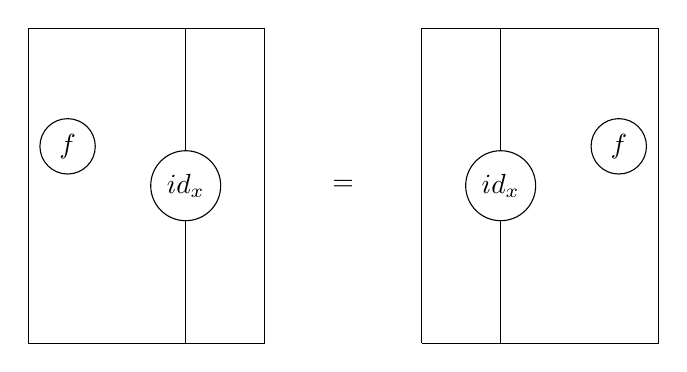
\begin{tikzpicture}
    \node(a) at (-0.5,0.5)[circle, fill=white, radius=2, draw]{$f$};
    \draw (1,2) -- (1,0) node[circle, fill=white, radius=22, draw]{$id_x$} -- (1,-2);
    \node at (3,0) {$=$};
    \node(b) at (6.5,0.5)[circle, fill=white, radius=2, draw]{$f$};
    \draw (5,2) -- (5,0) node[circle, fill=white, radius=22, draw]{$id_x$} -- (5,-2);
    \draw (-1,-2) -- (-1,2) -- (2,2) -- (2,-2) -- (-1,-2);
    \draw (4,-2) -- (4,2) -- (7,2) -- (7,-2) -- (4,-2);  
  \end{tikzpicture}
\end{center}
In a real-world version of these diagrams, we could use this detachedness to grab these endomorphisms and slide them over or under any strings we please, without affecting anything else in the diagram. This ability is embodied algebraically by the equation above, and hence categories which obey it are called `spacial'.

\begin{rem}
Beginning with the following lemma, the term \textit{action morphism}\index{action morphism} is used. This refers to the image of a morphism such as
  \[
    \alpha(g;f_1,\ldots,f_n)
  \]
where
  \[
    \alpha \colon \coprod_{n \in \mathbb{N}} P(n) \otimes_{\Lambda(n)} X^n \rightarrow X
  \]
is the action of a $\ML$-operad algebra for some $\ML$-operad $P$. Most often these action morphisms will be of the form
  \[
    \alpha(g;id_{x_1},\ldots,id_{x_{n}}).
  \]
Since we are most often in the setting of $\mb{Cat}$, then $\alpha$ will be a functor.
\end{rem}
\begin{lem}\label{spacial} If $\ML$ is a crossed action operad, then all $E\Lambda$-algebras are spacial.\end{lem}
\begin{proof}
Let $\ML$ be a crossed action operad, let $X$ be a $\ML$-monoidal category, and fix $x \in \mathrm{Ob}(X)$ and \( f\colon I \rightarrow I \). From \cref{surjortriv} we know that \( \pi \colon \Lambda(2) \rightarrow S_2 \) is surjective, so that the set $\pi^{-1}(  (1 \, 2)  )$ is non-empty,
% and from the uniqueness of action morphism composites (Lemma \ref{hom-set-lemma})
and from the rules for composition of action morphisms we see that for any such $g \in \pi^{-1}(  (1 \, 2)  )$,
  \begin{align*}
    \alpha(g  ;  \id_x,  \id_I  )\alpha(  e_2  ;  \id_x,  f  ) &= \alpha(ge_2 ; \id_x \id_x, \id_I f)\\
    &= \alpha(g  ;  \id_x, f) \\
    % &= \alpha(e_2 g; \id_x \id_x, f \id_I) \\
    &= \alpha(e_2; f, \id_x )\alpha(g; \id_x, \id_I). \\
  \end{align*}

Thus in order to obtain the result, it will suffice to find a particular $g \in \pi^{-1}( \, (1 \, 2) \, )$ for which
  \[
    \alpha(g; \id_x, \id_I) = \id_x.
  \]
However, since
  \begin{align*}
  		\alpha(  g  ;  \id_x,  \id_I  ) &= \alpha(  g  ;  \id_x,  \alpha( e_0; - )  ) \\
  		&= \alpha(  \mu(g; e_1, e_0)  ;  \id_x  )
		\end{align*}
all we need is to find a $g \in \pi^{-1}( \, (1 \, 2) \, )$ for which
  \[
    \mu(g; e_1, e_0) = e_1.
  \]
To this end, choose an arbitrary element $h \in \pi^{-1}( \, (1 \, 2) \, )$. This $h$ may not obey the above equation, but can be used to construct a new element, $g$, which does. Specifically, define
  \[
    k := \mu(h; e_1, e_0 )
  \]
and then consider
  \[
    g := h\mu\left(e_2; k^{-1}, e_1\right).
  \] 
To see that this is the correct choice of $g$, first note that we must have \( \pi(k) = e_1 \), since this is the only element of $S_1$. Following from that, we have 
  \begin{align*}
  	\pi \left(  \mu(e_2; k^{-1}, e_1)  \right) &= \mu \left(  \pi(e_2) \ ;  \pi\left(k^{-1}\right),  \pi(e_1)  \right) \\
  	&= \mu \left(  e_2  \ ;  e_1,  e_1  \right) \\
  	&= e_2
  \end{align*}
and hence
  \begin{align*}
		\pi(g) &= \pi \left(h \mu\left(e_2; k^{-1}, e_1\right) \right) \\
		       &= \pi(h) \pi \left(\mu\left(e_2; k^{-1}, e_1\right) \right) \\
		       &= (1 \, 2) e_2 \\
		       &= (1 \, 2).
  \end{align*}
So $g$ is indeed in $\pi^{-1}( \, (1 \, 2) \, )$, and furthermore
  \begin{align*}
  	\mu(g; e_1, e_0) & = \mu \left(  h \mu\left(e_2; k^{-1}, e_1\right) \ ;  e_1,  e_0  \right) \\
                  	 &= \mu(  h \ ;  e_1,  e_0  ) \mu \left(  \mu\left(e_2; k^{-1}, e_1\right) ;  e_1,  e_0   \right) \\
                  	 &= \mu(  h \ ;  e_1,  e_0  ) \mu \left(  e_2 \ ;  \mu\left(k^{-1}; e_1\right),  \mu(e_1;  e_0)  \right) \\
                  	 &= \mu(  h \ ;  e_1,  e_0  ) \mu\left(  e_2 \ ;  k^{-1}, e_0  \right) \\
                  	 &= k k^{-1} \\
                  	 &= e_1.
  \end{align*}
Therefore, $h \mu\left(e_2; k^{-1}, e_1\right)$ the required element $g$, and so working backwards through the proof we obtain the result. Since
  \[
    \mu(g; e_1, e_0) = e_1,
  \]
then
  \[
    \alpha(g;\id_x, \id_I) = \id_x.
  \]
Similarly,
  \[
    \alpha(g;\id_x, \id_I) \alpha(e_2; \id_x, f) = \alpha(e_2; f, \id_x) \alpha(g; \id_x, \id_I),
  \]
which gives
  \[
    \alpha(e_2; \id_x, f) = \alpha(e_2; f, \id_I).
  \]

\end{proof} 

\cref{hom-set-lemma} also gives a complete description of how the morphisms of $\ELn$ interact as a monoid under tensor product, though to best express this we need some new terminology.

\begin{Defi}\label{def:length} Let $\ML$ be an action operad. 
\begin{enumerate}
\item We will use the notation $\lop$ to denote the \emph{underlying monoid}\index{action operad!underlying monoid} of this action operad. The underlying set of $\lop$ is the disjoint union, $\coprod_n \Lambda(n)$, with block sum as the binary operation, $g \oplus h = \mu(e_2; g, h)$.

\item This monoid comes equipped with a homomorphism $| \, \_ \, | \colon \Lambda \rightarrow \mathbb{N}$, sending each $g \in \Lambda$ to the natural number $m$ if and only if $g$ is an element of the group $\Lambda(m)$. We call this number $|g|$ the \emph{length} of $g$.
\end{enumerate}
\end{Defi}

QQQ We have two different lengths which are sometimes the same, fix that. I want the free monoid length to be $\ell$ I think.

\begin{Defi}\label{lengthdef} Let $S$ be a set and $F(S)$ the free monoid on $S$, the monoid whose elements are strings of elements of $S$ and whose binary operation is concatenation. Then we will denote by
  \[
    | \, \_ \, | \colon F(S) \rightarrow \mathbb{N}
  \]
the monoid homomorphism defined by sending each element of $S \subseteq F(S)$ to 1, and therefore also each concatenation of $n$ elements of $S$ to the natural number $n$. Again, we will call $|x|$ the \emph{length} of $x \in F(S)$.
\end{Defi}

\begin{lem} \label{Gnmor} The monoid of morphisms of the algebra $\ELn$ is
  \[
    \mathrm{Mor}(\ELn) \quad \cong \quad \lop \times_{\mathbb{N}} \mathbb{N}^{\ast n}
  \]
where this is a pullback taken over the respective length homomorphisms,
  \[
    \begin{tikzcd}
      \lop \times_{\mathbb{N}} \mathbb{N}^{\ast n} \ar[dd, shift left=4] \ar[rr] \ar[ddrr, phantom, "\lrcorner", very near start, shift left] & & \mathbb{N}^{\ast n} \ar[dd, "| \, \_ \, |"] & \\
      & & & \\
      \quad \quad \Lambda \ar[rr, "| \, \_ \, |"] & & \mathbb{N} &
    \end{tikzcd}
  \]
using the fact that $\mathbb{N}^{\ast n}$ is the free monoid $F\left( \, \{z_1, \ldots, z_n\} \, \right)$.
\end{lem}
\begin{proof}
An element of $\Lambda \times_{\mathbb{N}} F( \, \{z_1, \ldots, z_n\} \, )$ is an element $g \in \Lambda(m)$ for some $m$, together with an $m$-tuple of objects $(x_1, \ldots, x_m)$ from the set of generators $\{z_1, \ldots, z_n\}$. Thus the action on $\ELn$ defines a function 
% \[ \begin{array}{rlrll}
% 			\alpha & \colon & \Lambda \times_{\mathbb{N}} F\left( \, \{z_1, \ldots, z_n\} \, \right) & \rightarrow & \mathrm{Mor}(\ELn) \\
% 			& \colon & (g;x_1, \ldots, x_m) & \mapsto & \alpha(g; \id_{x_1}, \ldots, \id_{x_m})
% 		\end{array}
% \]
\begin{align*}
    \alpha \colon \Lambda \times_{\mathbb{N}} F\left( \, \{z_1, \ldots, z_n\} \, \right) &\rightarrow \mathrm{Mor}(\ELn) \\
    (g;x_1, \ldots, x_m) &\mapsto \alpha(g; \id_{x_1}, \ldots, \id_{x_m})
\end{align*}
But by \cref{hom-set-lemma}, each element of $\mathrm{Mor}(\ELn)$ can be expressed in the form $\alpha(g; \id_{x_1}, \ldots, \id_{x_m})$ for a unique collection $(g;x_1, \ldots, x_m)$, and so this function $\alpha$ is actually a bijection of sets. Furthermore, this function preserves tensor product, since
  \begin{align*}
  		\alpha\left( \, (g;f_1, \ldots, f_m) \otimes (g';f'_1, \ldots, f'_m) \, \right) &= \alpha\left( \, g \otimes g' \, ; \, f_1, \ldots, f_m, f'_1, \ldots, f'_m \, \right) \\
  		&= \alpha\left( \, g \, ; \, f_1, \ldots, f_m \, \right) \otimes \alpha\left( \, g' \, ; \, f'_1, \ldots, f'_m \right)
  \end{align*}
and hence it is a monoid isomorphism, as required.
\end{proof}

\section{Pseudo-commutativity}

This section gives conditions sufficient to equip the 2-monad $\underline{P}$ induced by a $\ML$-operad $P$ in $\mb{Cat}$ with a pseudo-commutative structure.  Such a pseudo-commutativity will then give the 2-category $\mb{Ps}\mbox{-}\underline{P}\mbox{-}\mb{Alg}$ some additional structure that we briefly explain here.  For a field $k$, the category $\mb{Vect}$\nomenclature[C]{$\mb{Vect}$}{of vector spaces over a given field $k$ and $k$-linear maps} of vector spaces over $k$ has many nice features.  Of particular interest to us are the following three structures.  First, the category $\mb{Vect}$ is monoidal using the tensor product $\otimes_{k}$.  Second, the set of linear maps $V \rightarrow W$ is itself a vector space which we denote $[V,W]$.  Third, there is a notion of multilinear map\index{multilinear map} $V_{1} \times \cdots \times V_{n} \rightarrow W$, with linear maps being the 1-ary version.  While these three structures are each useful in isolation, they are tied together by natural isomorphisms
  \[
    \mb{Vect}(V_{1} \otimes V_{2}, W) \cong \mb{Vect}(V_{1}, [V_{2}, W]) \cong \mb{Bilin}(V_{1} \times V_{2}, W)
  \]
expressing that $\otimes$ gives a closed monoidal structure which represents the multicategory of multilinear maps.  Moreover, the adjunction between $\mb{Vect}$ and $\mb{Sets}$ respects all of this structure in the appropriate way.  This incredibly rich interplay between the tensor product, the internal mapping space, and the multicategory of multilinear maps all arises from the free vector space monad on $\mb{Sets}$ being a \textit{commutative} monad \cite{kock-monads, kock-closed, kock-strong}.  The notion of a pseudo-commutative 2-monad \cite{HP} is then a generalization of this machinery to a 2-categorical context, and can be viewed as a starting point for importing tools from linear algebra into category theory.

The aim of this section is to give conditions that ensure that the 2-monad $\underline{P}$ associated to a $\ML$-operad $P$ has a pseudo-commutative structure. We give the definition of pseudo-commutativity as in \cite{HP} but before doing so we require the definition of a strength for a $2$-monad.
\begin{Defi}
A \textit{strength}\index{$2$-monad!strength} for an endo-$2$-functor $T \colon \m{K} \rightarrow \m{K}$ on a 2-category with products and terminal object $1$ consists of a $2$-natural transformation $d$ with components
    \[
        d_{A,B} \colon A \times TB \rightarrow T(A \times B)
    \]
satisfying the following unit and associativity axioms \cite{kock-monads}.
  \[
    \xy
    (0,0)*+{1 \times TA}="ul1";
    (30,0)*+{T(1 \times A)}="ur1";
    (30,-13)*+{TA}="br1";
    (50,0)*+{A \times B}="ul2";
    (80,0)*+{A \times TB}="ur2";
    (80,-13)*+{T(A \times B)}="br2";
    {\ar^{d_{1,A}} "ul1"; "ur1"};
    {\ar^{\cong} "ur1"; "br1"};
    {\ar_{\cong} "ul1"; "br1"};
    {\ar^{1 \times \eta} "ul2"; "ur2"};
    {\ar^{d_{A,B}} "ur2"; "br2"};
    {\ar_{\eta} "ul2"; "br2"};
    \endxy
  \]
  \[
    \xy
    (0,0)*+{(A \times B) \times TC}="ul";
    (70,0)*+{T \left((A \times B) \times C \right)}="ur";
    (0,-15)*+{A \times (B \times TC)}="ll";
    (35,-15)*+{A \times T(B \times C)}="m";
    (70,-15)*+{ T \left(A \times (B \times C) \right)}="lr";
    {\ar^{d_{AB,C}} "ul"; "ur"};
    {\ar^{Ta} "ur"; "lr"};
    {\ar_{a} "ul"; "ll"};
    {\ar_{1 \times d_{B,C}} "ll"; "m"};
    {\ar_{d_{A,BC}} "m"; "lr"};
    \endxy
  \]
  \[
    \xy
    (0,0)*+{A \times T^{2}B}="ul";
    (60,0)*+{T^{2}(A \times B)}="ur";
    (0,-15)*+{A \times TB}="ll";
    (30,0)*+{T(A \times TB)}="m";
    (60,-15)*+{ T(A \times B)}="lr";
    {\ar^{d_{A,TB}} "ul"; "m"};
    {\ar^{Td_{A,B}} "m"; "ur"};
    {\ar^{\mu} "ur"; "lr"};
    {\ar_{1 \times \mu} "ul"; "ll"};
    {\ar_{d_{A,B}} "ll"; "lr"};
    \endxy
  \]
Similarly, a \emph{costrength}\index{$2$-monad!costrength} for $T$ consists of a $2$-natural transformation $d^{\ast}$ with components
  \[
      d^{\ast}_{A,B} \colon TA \times B \rightarrow T(A \times B)
  \]
again satisfying unit and associativity axioms.
\end{Defi}
The strength and costrength for the associated $2$-monad $\underline{P}$ are quite simple to define. We define the strength $d$ for $\underline{P}$ as follows. The component $d_{A,B}$ is a functor
    \[
        d_{A,B} \colon A \times \left(\amalg P(n) \times_{\Lambda(n)} B^n\right) \rightarrow \amalg P(n) \times_{\Lambda(n)} \left(A \times B \right)^n
    \]
which sends an object $(a, [p;b_1,\ldots,b_n])$ to the object $[p;(a,b_1),\ldots,(a,b_n)]$. We also define the costrength similarly, sending an object $([p;a_1,\ldots,a_n],b)$ to the object $[p;(a_1,b), \ldots, (a_n, b)]$. Both the strength and the costrength are defined in the obvious way on morphisms.

\begin{rem}
It is crucial to note that the strength $d$ and the costrength $d^{*}$ do not depend on the $\Lambda$-actions in the following sense.  The $\ML$-operad $P$ has an underlying non-symmetric operad that we also denote $P$, and it has a strength
  \[
    d_{A,B} \colon A \times \left(\amalg P(n) \times B^n\right) \rightarrow \amalg P(n) \times \left(A \times B \right)^n
  \]
given by essentially the same formula:
  \[
    \left( a; (p; b_{1}, \ldots, b_{n}) \right) \mapsto \left(p; (a,b_{1}), \ldots, (a, b_{n})\right).
  \]
The strength for the $\Lambda$-equivariant $P$ is just the induced functor between coequalizers.
\end{rem}

\begin{Defi}
    Given a $2$-monad $T \colon \m{K} \rightarrow \m{K}$ with strength $d$ and costrength $d^{\ast}$, a \textit{pseudo-commutativity}\index{$2$-monad!pseudo-commutativity} consists of an invertible modification $\gamma$ with components
      \[
        \xy
            (0,0)*+{TA \times TB}="00";
            (30,0)*+{T(A \times TB)}="10";
            (60,0)*+{T^2(A \times B)}="20";
            (0,-15)*+{T(TA \times B)}="01";
            (30,-15)*+{T^2(A \times B)}="11";
            (60,-15)*+{T(A \times B)}="21";
            {\ar^{d^{\ast}_{A,TB}} "00" ; "10"};
            {\ar^{Td_{A,B}} "10" ; "20"};
            {\ar^{\mu_{A \times B}} "20" ; "21"};
            {\ar_{d_{TA,B}} "00" ; "01"};
            {\ar_{Td^{\ast}_{A,B}} "01" ; "11"};
            {\ar_{\mu_{A \times B}} "11" ; "21"};
            {\ar@{=>}^{\gamma_{A,B}} (30,-5.5) ; (30,-9.5)};
        \endxy
      \]
satisfying the following three strength axioms, two unit (or $\eta$) axioms, and two multiplication (or $\mu$) axioms for all $A$, $B$, and $C$.
    \begin{enumerate}
        \item $\gamma_{A \times B,C} * (d_{A,B} \times 1_{TC}) = d_{A,B \times C} * (1_A \times \gamma_{B,C})$
        \item $\gamma_{A,B \times C} * (1_{TA} \times d_{B,C}) = \gamma_{A \times B, C} * (d^{\ast}_{A,B} \times 1_{TC})$
        \item $\gamma_{A,B \times C} * (1_{TA} \times d^{\ast}_{B,C}) = d^{\ast}_{A \times B,C} * (\gamma_{A,B} \times 1_{C})$
        \item $\gamma_{A,B} * (\eta_A \times 1_{TB})$  is the identity on $d$.
        \item $\gamma_{A,B} * (1_{TA} \times \eta_B)$ is the identity on $d^{*}$.
        \item $\gamma_{A,B} * (\mu_A \times 1_{TB})$ is equal to the pasting below.
          \[
            \xy
                (0,0)*+{\scriptstyle T^2A \times TB}="00";
                (30,0)*+{\scriptstyle T(TA \times TB)}="10";
                (60,0)*+{\scriptstyle T^2(A \times TB)}="20";
                (90,0)*+{\scriptstyle T^3(A \times B)}="30";
                (0,-15)*+{\scriptstyle T(T^2A \times B)}="01";
                (30,-15)*+{\scriptstyle T^2(TA \times B)}="11";
                (60,-15)*+{\scriptstyle T^3(A \times B)}="21";
                (90,-15)*+{\scriptstyle T^2(A \times B)}="31";
                (0,-30)*+{\scriptstyle T^2(TA \times B)}="02";
                (30,-30)*+{\scriptstyle T(TA \times B)}="12";
                (60,-30)*+{\scriptstyle T^2(A \times B)}="22";
                (90,-30)*+{\scriptstyle T(A \times B)}="32";
                {\ar^{d^{\ast}_{TA,TB}} "00" ; "10"};
                {\ar^{Td^{\ast}_{A,TB}} "10" ; "20"};
                {\ar^{T^2 d_{A,B}} "20" ; "30"};
                {\ar_{d_{T^2A,B}} "00" ; "01"};
                {\ar_{Td_{TA,B}} "10" ; "11"};
                {\ar^{T\mu_{A \times B}} "30" ; "31"};
                {\ar_{T^2 d^{\ast}_{A,B}} "11" ; "21"};
                {\ar_{T\mu_{A \times B}} "21" ; "31"};
                {\ar_{Td^{\ast}_{TA,B}} "01" ; "02"};
                {\ar_{\mu_{TA \times B}} "11" ; "12"};
                {\ar_{\mu_{T(A \times B)}} "21" ; "22"};
                {\ar^{\mu_{A \times B}} "31" ; "32"};
                {\ar_{\mu_{TA \times B}} "02" ; "12"};
                {\ar_{Td^{\ast}_{A,B}} "12" ; "22"};
                {\ar_{\mu_{A \times B}} "22" ; "32"};
                {\ar@{=>}^{T\gamma_{A,B}} (60,-5.5) ; (60,-9.5)};
                {\ar@{=>}^{\gamma_{TA,B}} (12.5,-13) ; (12.5,-17)};
            \endxy
          \]
        \item $\gamma_{A,B} * (1_{TA} \times \mu_B)$ is equal to the pasting below.
          \[
            \xy
                (0,0)*+{\scriptstyle TA \times T^2B}="00";
                (30,0)*+{\scriptstyle T(A \times T^2B)}="10";
                (60,0)*+{\scriptstyle T^2(A \times TB)}="20";
                (0,-15)*+{\scriptstyle T(TA \times TB)}="01";
                (30,-15)*+{\scriptstyle T^2(A \times TB)}="11";
                (60,-15)*+{\scriptstyle T(A \times TB)}="21";
                (0,-30)*+{\scriptstyle T^2(TA \times B)}="02";
                (30,-30)*+{\scriptstyle T^3(A \times B)}="12";
                (60,-30)*+{\scriptstyle T^2(A \times B)}="22";
                (0,-45)*+{\scriptstyle T^3(A \times B)}="03";
                (30,-45)*+{\scriptstyle T^2(A \times B)}="13";
                (60,-45)*+{\scriptstyle T(A \times B)}="23";
                {\ar^{d^{\ast}_{A,T^2B}} "00" ; "10"};
                {\ar^{Td_{A,TB}} "10" ; "20"};
                {\ar_{d_{TA,TB}} "00" ; "01"};
                {\ar^{\mu_{A \times TB}} "20" ; "21"};
                {\ar_{Td^{\ast}_{A,TB}} "01" ; "11"};
                {\ar_{\mu_{A \times TB}} "11" ; "21"};
                {\ar_{Td_{TA,B}} "01" ; "02"};
                {\ar^{T^2 d_{A,B}} "11" ; "12"};
                {\ar^{Td_{A,B}} "21" ; "22"};
                {\ar^{\mu_{T(A \times B)}} "12" ; "22"};
                {\ar_{T^2 d^{\ast}_{A,B}} "02" ; "03"};
                {\ar^{T\mu_{A \times B}} "12" ; "13"};
                {\ar^{\mu_{A \times B}} "22" ; "23"};
                {\ar_{T\mu_{A \times B}} "03" ; "13"};
                {\ar_{\mu_{A \times B}} "13" ; "23"};
                {\ar@{=>}^{T\gamma_{A,B}} (13,-28) ; (13,-32)};
                {\ar@{=>}^{\gamma_{A,TB}} (30,-5.5) ; (30,-9.5)};
            \endxy
          \]
    \end{enumerate}
\end{Defi}

\begin{rem}
    It is noted in \cite{HP} that this definition has some redundancy and therein it is shown that any two of the strength axioms immediately implies the third. Furthermore, the three strength axioms are equivalent when the $\eta$ and $\mu$ axioms hold, as well as the following associativity axiom:
        \[
            \gamma_{A,B \times C} \circ (1_{TA} \times \gamma_{B,C}) = \gamma_{A \times B,C} \times (\gamma_{A,B} \times 1_{TC}).
        \]
\end{rem}

We need some further notation before stating our main theorem.  Let $\underline{a} = a_{1}, \ldots , a_{m}$ and $\underline{b} = b_{1}, \ldots, b_{n}$ be two lists.  Then the set $\{ (a_{i}, b_{j})\}$ has $mn$ elements, and two natural lexicographic orderings.  One of these we write as $\underline{(a, \underline{b})}$, and it has the order given by
  \[
    (a_{p}, b_{q}) < (a_{r}, b_{s}) \textrm{ if } \left\{ \begin{array}{l} p < r, \textrm{ or } \\ p=r \textrm{ and } q < s. \end{array} \right.
  \]
The other we write as $\underline{(\underline{a}, b)}$, and it has the order given by
\[
    (a_{p}, b_{q}) < (a_{r}, b_{s}) \textrm{ if } \left\{ \begin{array}{l} q < s, \textrm{ or } \\ q=s \textrm{ and } p < r. \end{array} \right.
  \]
The notation $(a, \underline{b})$ is meant to indicate that we have a single $a$ but a list of $b$'s, so then $\underline{(a, \underline{b})}$ would represent a list which itself consists of lists of that form. There is a unique permutation $\tau_{m,n} \in \Sigma_{mn}$ which has the property that $\tau_{m,n}(i) = j$ if the $i$th element of the ordered set $\underline{(a, \underline{b})}$ is equal to the $j$th element of the ordered set $\underline{(\underline{a}, b)}$.  By construction, we have $\tau_{n,m} = \tau_{m,n}^{-1}$. We illustrate these permutations with a couple of examples.
    \[
        \xy
            {\ar@{-} (0,0) ; (0,-10)};
            {\ar@{-} (5,0) ; (10,-10)};
            {\ar@{-} (10,0) ; (20,-10)};
            {\ar@{-} (15,0) ; (5,-10)};
            {\ar@{-} (20,0) ; (15,-10)};
            {\ar@{-} (25,0) ; (25,-10)};
            (12.5,-13)*{\tau_{2,3}};
            {\ar@{-} (45,0) ; (45,-10)};
            {\ar@{-} (50,0) ; (65,-10)};
            {\ar@{-} (55,0) ; (50,-10)};
            {\ar@{-} (60,0) ; (70,-10)};
            {\ar@{-} (65,0) ; (55,-10)};
            {\ar@{-} (70,0) ; (75,-10)};
            {\ar@{-} (75,0) ; (60,-10)};
            {\ar@{-} (80,0) ; (80,-10)};
            (62.5,-13)*{\tau_{4,2}}
        \endxy
    \]
Note then that $\tau_{m,n}$ is the permutation given by taking the transpose of the $m \times n$ matrix with entries $(a_{i}, b_{j})$.


We now give sufficient conditions for equipping the 2-monad $\underline{P}$ associated to a $\ML$-operad $P$ with a pseudo-commutative structure.  Let $\mathbb{N}_{+}$ denote the set of positive natural numbers.
\begin{thm}\label{pscomm}
Let $P$ be a $\ML$-operad. Then the following equip $\underline{P}$ with a pseudo-commutative structure.
    \begin{itemize}
        \item For each pair $(m,n) \in \mathbb{N}_{+}^2$, we are given an element $t_{m,n} \in \Lambda(mn)$ such that $\pi(t_{m,n}) = \tau_{m,n}$.
        \item For each $p \in P(n)$, $q \in P(m)$, we are given a natural isomorphism
            \[
                \lambda_{p,q} \colon \mu(p;q,\ldots,q) \cdot t_{m,n} \cong \mu(q;p,\ldots,p).
            \]
            We write this as $\lambda_{p,q}\colon \mu(p; \underline{q}) \cdot t_{m,n} \cong \mu(q; \underline{p})$.
    \end{itemize}
These must satisfy the following:  
    \begin{enumerate}
        \item For all $n \in \mathbb{N}_+$\nomenclature[N]{$\mathbb{N}_+$}{the set of positive natural numbers},
            \[
                t_{1,n} = e_n = t_{n,1}
            \]
             and for all $p \in P(n)$, the isomorphism $\lambda_{p, \id}\colon p \cdot e_n \cong p$ is the identity map.
        \item For all $l, m_1, \ldots, m_l, n \in \mathbb{N}_+$, with $M = \Sigma m_i$,
            \[
                \mu^{\Lambda}\left(e_l; t_{m_1,n}, \ldots, t_{m_l,n}\right) \cdot \mu^{\Lambda}\left(t_{l,n};\underline{e_{m_1},\ldots,e_{m_l}}\right) = t_{n,M}.
            \]
            Here $\underline{e_{m_1},\ldots,e_{m_l}}$ is the list $e_{m_{1}}, \ldots, e_{m_{l}}$ repeated $n$ times.
        \item For all $l, m, n_1,\ldots, n_m \in \mathbb{N}_+$, with $N = \Sigma n_i$,
            \[
                \mu^{\Lambda}\left(t_{m,l};\underline{e_{n_1}},\ldots,\underline{e_{n_m}}\right) \cdot \mu^{\Lambda}\left(e_m;t_{n_1,l},\ldots,t_{n_m,l}\right) = t_{N,l}.
            \]
            Here $\underline{e_{n_{i}}}$ indicates that each $e_{n_{i}}$ is repeated $l$ times.
        \item For any $l, m_i, n \in \mathbb{N}_+$, with $1 \leq i \leq n$, and $p \in P(l)$, $q_i \in P(m_i)$ and $r \in P(n)$, the following diagram commutes.  (Note that we maintain the convention that anything underlined indicates a list, and double underlining indicates a list of lists.  Each instance should have an obvious meaning from context and the equations appearing above.)
          \[
            \xy
                (0,0)*+{\mu\left(p;\underline{\mu(q_i;\underline{r})}\right) \cdot \mu(e_l;\underline{t_{n,m_i}})\mu(t_{n,l};\underline{\underline{e_{m_i}}})}="00";
                (60,0)*+{\mu\left(p;\underline{\mu(q_i;\underline{r})}\right) \cdot t_{n,M}}="10";
                (0,-15)*+{\mu\left(p;\underline{\mu(q_i;\underline{r})\cdot t_{n,m_i}}\right) \cdot \mu(t_{n,l};\underline{e_{m_1},\ldots,e_{m_l}})}="01";
                (60,-20)*+{\mu\left(\mu(p;q_1,\ldots,q_n);\underline{\underline{r}}\right)\cdot t_{n,M}}="11";
                (0,-30)*+{\mu\left(p;\underline{\mu(r;\underline{q_i})}\right) \cdot \mu(t_{n,l};\underline{e_{m_1},\ldots,e_{m_l}})}="02";
                (60,-40)*+{\mu\left(\mu(p;q_1,\ldots,q_n);\underline{\underline{r}}\right)}="12";
                (0,-45)*+{\mu\left(\mu(p;\underline{r}) \cdot t_{n,l} ; \underline{q_1,\ldots,q_n}\right)}="03";
                (60,-60)*+{\mu\left(r;\underline{\mu(p;q_1,\ldots,q_n)}\right)}="13";
                (0,-60)*+{\mu\left(\mu(r,\underline{p});\underline{q_1,\ldots,q_n}\right)}="04";
                {\ar@{=} "00" ; "10"};
                {\ar@{=} "00" ; "01"};
                {\ar@{=} "10" ; "11"};
                {\ar_{\mu(1;\underline{\lambda_{q_i,r}}) \cdot 1} "01" ; "02"};
                {\ar@{=} "02" ; "03"};
                {\ar@{=} "04" ; "13"};
                {\ar_{\mu(\lambda_{p,r};1)} "03" ; "04"};
                {\ar^{\lambda_{\mu(p;q_1,\ldots,q_n),r}} "11" ; "12"};
                {\ar@{=} "12" ; "13"};
            \endxy
          \]
        \item For any $l,m, n_i \in \mathbb{N}_+$, with $1 \leq i \leq m$, and $p \in P(l)$, $q \in P(m)$ and $r_i \in P(n_i)$, the following diagram commutes.
          \[
            \xy
                (0,0)*+{\mu\left(\mu(p;\underline{q}) \cdot t_{m,l} ; \underline{\underline{r_i}}\right) \cdot \mu(e_m;\underline{t_{n_i,l}})}="00";
                (60,0)*+{\mu\left(\mu(p;\underline{q});\underline{\underline{r_i}}\right) \cdot \mu(t_{m,l};\underline{\underline{e_{n_i}}})\mu(e_{m};\underline{t_{n_i,l}})}="10";
                (60,-15)*+{\mu\left(p;\underline{\mu(q;\underline{r_i})}\right) \cdot \mu(t_{m,l};\underline{\underline{e_{n_i}}})\mu(e_{m};\underline{t_{n_i,l}})}="11";
                (0,-20)*+{\mu\left(\mu(q;\underline{p}); \underline{r_1},\ldots,\underline{r_m}\right) \cdot \mu(e_m;\underline{t_{n_i,l}})}="01";
                (0,-40)*+{\mu\left(q;\underline{\underline{\mu(p;r_i)}}\right) \cdot \mu(e_m;\underline{t_{n_i,l}})}="02";
                (0,-60)*+{\mu\left(q;\underline{\mu(p;\underline{r_i}) \cdot t_{n_i,l}}\right)}="03";
                (60,-30)*+{\mu\left(p;\underline{\mu(q;r_1,\ldots,r_m)}\right) \cdot t_{N,l}}="12";
                (60,-45)*+{\mu\left(\mu(q;r_1,\ldots,r_m); \underline{\underline{p}}\right)}="13";
                (60,-60)*+{\mu\left(q;\underline{\mu(r_i;\underline{p})}\right)}="14";
                {\ar@{=} "00" ; "10"};
                {\ar@{=} "10" ; "11"};
                {\ar@{=} "11" ; "12"};
                {\ar^{\lambda_{p,\mu(q;r_1,\ldots,r_m)}} "12" ; "13"};
                {\ar@{=} "13" ; "14"};
                {\ar_{\mu(\lambda_{p,q};1) \cdot 1} "00" ; "01"};
                {\ar@{=} "01" ; "02"};
                {\ar@{=} "02" ; "03"};
                {\ar_{\mu(1;\underline{\lambda_{p,r_i}})} "03" ; "14"};
            \endxy
          \]
    \end{enumerate}
\end{thm}

\begin{proof}
We begin the proof by defining an invertible modification $\gamma$ for the pseudo-commutativity for which the components are natural transformations $\gamma_{A,B}$.  Such a transformation $\gamma_{A,B}$ has components with source
  \[
    \left[\mu\left(p; \underline{q}\right); \underline{(x, \underline{y})}\right]
  \]
and target
  \[
    \left[\mu\left(q; \underline{p}\right); \underline{(\underline{x},y)}\right].
  \]
Now $ \lambda_{p,q} \colon \mu(p;q,\ldots,q) \cdot t_{m,n} \cong \mu(q;p,\ldots,p)$ gives rise to another map by multiplication on the right by $t_{m,n}^{-1}$,
  \[
    \lambda_{p,q}\cdot t_{m,n}^{-1} \colon \mu(p;q,\ldots,q) \cong \mu(q;p,\ldots,p) \cdot t_{m,n}^{-1},
  \]
so we define $(\gamma_{A,B})_{[p;a_1,\ldots,a_n],[q;b_1,\ldots,b_m]}$ to be the morphism which is the image of $(\lambda_{p,q}\cdot t_{m,n}^{-1}, 1)$ under the map
  \[
    \coprod P(n) \times (A \times B)^{n} \rightarrow \coprod P(n) \times_{\Lambda(n)} (A \times B)^{n}.
  \]
We will write this morphism as $[\lambda_{p,q}t_{m,n}^{-1}, 1]$.  In the case that either $p$ or $q$ is an identity then we choose the component of $\gamma$ to be the isomorphism involving the appropriate identity element using axiom 1 above.

There are two things to note about the definition above before we continue.  First, it is easy to check that
  \[
    t_{m,n}^{-1} \cdot \underline{\left(x, \underline{y}\right)} = \underline{\left(\underline{x},y\right)}
  \]
since $\pi(t_{m,n}) = \tau_{m,n}$; this ensures that $\gamma$ has the correct target.  Second, the morphism above has second component the identity.  This is actually forced upon us by the requirement that $\gamma$ be a modification:  in the case that $A,B$ are discrete categories, the only possible morphism is an identity, and the modification axiom then forces that statement to be true for general $A,B$ by considering the inclusion $A_{0} \times B_{0} \hookrightarrow A \times B$ where $A_{0}, B_{0}$ are the discrete categories with the same objects as $A, B$.

We show that this is a modification by noting that it does not rely on objects in the lists $a_1, \ldots, a_n$ or $b_1, \ldots, b_m$, only on their lengths and the operations $p$ and $q$. As a result, if we have functors $f \colon X \rightarrow X'$ and $g \colon Y \rightarrow Y'$, then it is clear that
    \[
        (\underline{P}(f\times g) \circ \gamma_{X,Y})_{\left[p;\underline{x}\right],\left[q;\underline{y}\right]} = [\lambda_{p,q},\underline{1}] = (\gamma_{X',Y'} \circ (\underline{P}f\times \underline{P}g))_{\left[p;\underline{x}\right],\left[q;\underline{y}\right]}.
    \]
As such we can simply write $(\gamma_{X,Y})_{[p;\underline{x}],[q;\underline{y}]}$ in shorthand as $\gamma_{p,q}$.

There are now seven axioms to check for a pseudo-commutativity:  three strength axioms, two unit axioms, and two multiplication axioms.  For the first strength axiom, we must verify that two different 2-cells of shape
  \[
    \xy
      (0,0)*+{A \times TB \times TC}="0";
      (50,0)*+{T(A \times B \times C)}="1";
      {\ar@/^1pc/ "0"; "1"};
      {\ar@/_1pc/ "0"; "1"};
      (25,0)*{\Downarrow}
    \endxy
  \]
are equal.  The first of these is $\gamma$ precomposed with $d \times 1$, and so is the component of $\gamma$ at an object
  \[
    \left( [p;(a,b_1),\ldots,(a,b_n)], [q; c_{1}, \ldots, c_{m}] \right).
  \]
The second of these is $d$ applied to the component of $1 \times \gamma$ at
  \[
    \left(a, ([p;b_1,\ldots,b_n], [q; c_{1}, \ldots, c_{m}]) \right).
  \]
It is straightforward to compute that each of these maps is the image of $\left(\lambda_{p,q}\cdot t_{m,n}^{-1},1\right)$ under the functor
  \[
    \coprod P(n) \times (A \times B)^{n} \rightarrow \coprod P(n) \times_{\Lambda(n)} (A \times B)^{n}.
  \]
The other two strength axioms follow by analogous calculations for other whiskerings of $\gamma$ with $d$ or $d^{*}$.


For the unit axioms, we must compute the components of $\gamma$ precomposed with $\eta \times 1$ for the first axiom and $1 \times \eta$ for the second.  Thus for the first unit axiom, we must compute the component of $\gamma$ at $\left( [e;a], [p; b_{1}, \ldots, b_{m}] \right)$.  By definition, this is the image of $(\lambda_{e,p}\cdot t^{-1}_{m,1}, 1)$ under the map to the coequalizer, and by the first hypothesis of the theorem we know that $t^{-1}_{m,1}$ is the identity element and this isomorphism is the identity as well, so this component of $\gamma$ is also the identity.  The second unit axiom follows similarly, using that $t^{-1}_{1,n}$ is the identity.


For the multiplication axioms, first note that hypothesis 2 in the statement of the theorem is necessary in order to ensure the existence of the top horizontal equality in the diagram of hypothesis 4; the same goes for hypotheses 3 and 5. We now explain how hypotheses 2 and 4 ensure that the first multiplication axiom holds, with the same reasoning showing that hypotheses 3 and 5 imply the second multiplication axiom.

We begin by studying the pasting diagram in the first multiplication axiom, but computing its values using the strength and costrength for the non-symmetric operad underlying $P$; this means that we evaluate on objects of the form $(p; a_{1}, \ldots, a_{n})$ rather than on their equivalence classes.  Let $p \in P(l), q_{i} \in P(m_{i})$ for $1 \leq i \leq l$, and $r \in P(n)$. Computing the top and right leg around the pasting diagram gives the function on objects which sends
  \[
    \left( (p; (q_{1}; \un{a_{1}}), \ldots, (q_{l}; \un{a_{l}})), (r; \un{b}) \right)
  \]
to
  \[
    \left( \mu(p; \mu(q_{1}; \un{r}), \ldots, \mu(q_{l}; \un{r})); (\un{(a_{1\bullet}, \un{b})}), \ldots, (\un{(a_{l\bullet}, \un{b})}) \right),
  \]
where $(\un{(a_{i\bullet}, \un{b})})$ is the list of pairs
  \[
    (a_{i1}, b_{1}), \ldots, (a_{i1}, b_{m}), (a_{i2}, b_{1}), \ldots, (a_{in_{i}}, b_{m}).
  \]
Then $\un{P}\gamma$ is the image of the morphism which is the identity on the $(a_{ij}, b_{k})$'s, and is the morphism
  \[
    \mu\left(1;\lambda_{q1,r}t^{-1}_{n,m_1},\ldots,\lambda_{q1,r}t^{-1}_{n,m_l}\right)
  \]
on the first component with domain and codomain shown below.
  \[
    \mu\left(p;\mu\left(q_1;\un{r}\right),\ldots,\mu\left(q_n;\un{r}\right)\right) \longrightarrow \mu\left(p;\mu\left(r;\un{q_1}\right)t^{-1}_{n,m_1},\ldots,\mu\left(r;\un{q_l}\right)t^{-1}_{n,m_l}\right)
  \]
% \[
% \xy
% {\ar^{\scriptstyle \mu\left(1; \lambda_{q_{1}, r} t^{-1}_{n,m_{1}}, \ldots, \lambda_{q_{1}, r} t^{-1}_{n,m_{l}}\right)} (0,0)*+{\scriptstyle \mu\left(p; \mu(q_{1}; \un{r}), \ldots, \mu(q_{n}; \un{r})\right)}; (75,0)*+{\scriptstyle \mu\left(p; \mu(r; \un{q_{1}}) t^{-1}_{n,m_{1}}, \ldots, \mu(r; \un{q_{l}}) t^{-1}_{n,m_{l}} \right)} }
% \endxy
% \]
% on the first component. 
By the $\Lambda$-operad axioms, the target of this morphism is equal to
  \[
    \mu\left(p; \mu\left(r; \un{q_{1}}\right), \ldots, \mu\left(r; \un{q_{l}}\right) \right)\mu\left(e_{l}; t^{-1}_{n,m_{1}}, \ldots, t^{-1}_{n,m_{l}}\right).
  \]
Note that this is not the same object as one obtains by computing $T\mu \circ T^{2}d^{*} \circ Td \circ d^{*}$ using the underlying non-symmetric operad of $P$ as we are required to use the $\Lambda$-equivariance to ensure that the target of $\gamma$ is the correct one.

Next we compute the source of $(\mu \circ Td^{*})*\gamma$, the other 2-cell in the pasting appearing in the first multiplication axiom.  We compute this once again using the strength and costrength for the underlying non-symmetric operad, and note once again that this will not match our previous calculations precisely, but only up to an application of $\Lambda$-equivariance.  This functor has its map on objects given by
  \[
    \left( (p; (q_{1}; \un{a_{1}}), \ldots, (q_{l}; \un{a_{l}})), (r; \un{b}) \right) \mapsto \left(\mu(\mu(p; \un{r}); \un{q_{1}}, \ldots, \un{q_{l}}); \un{(\un{a_{1}}, b_{\bullet})}, \ldots, \un{(\un{a_{l}}, b_{\bullet})} \right).
  \]
  Note that if we apply $\Lambda$-equivariance, this matches the target computed above. Once again the component of $\gamma$ is the image of a morphism which is the identity on the $(a_{ij}, b_{k})$'s, and its first component is
  \[
    \xy
      {\ar^{\mu\left(\lambda_{p,r} \cdot t^{-1}_{n,l}; 1, \ldots, 1\right)} (0,0)*+{\mu\left(\mu(p; \un{r}); \un{q_{1}}, \ldots, \un{q_{l}}\right)}; (60,0)*+{\mu\left(\mu(r; \un{p})\cdot t^{-1}_{n,l}; \un{q_{1}}, \ldots, \un{q_{l}}\right).} }
    \endxy
  \]

We cannot compose these morphisms in $\coprod P(n) \times (A \times B)^{n}$ as they do not have matching source and target, but we can in $\coprod P(n) \times_{\Lambda} (A \times B)^{n}$.  The resulting morphism has first component given by the image of
  \[
    \xy
      {\ar^{\scriptstyle \mu\left(1; \lambda_{q_{1}, r} t^{-1}_{n,m_{1}}, \ldots, \lambda_{q_{1}, r} t^{-1}_{n,m_{l}}\right)} (0,0)*+{\scriptstyle \mu\left(p; \mu\left(q_{1}; \un{r}\right), \ldots, \mu\left(q_{n}; \un{r}\right)\right)}; (75,0)*+{\scriptstyle \mu\left(p; \mu\left(r; \un{q_{1}}\right) t^{-1}_{n,m_{1}}, \ldots, \mu\left(r; \un{q_{l}}\right) t^{-1}_{n,m_{l}} \right)} };
      {\ar^<<<<<<<<<<<<<<<<<<<<<<{\scriptstyle \mu\left(\lambda_{p,r} \cdot t^{-1}_{n,l}; 1, \ldots, 1\right)\cdot \mu\left(e_{l}; t^{-1}_{n,m_{1}}, \ldots, t^{-1}_{n,m_{l}}\right)} (0,-10)*+{}; (75,-10)*+{\scriptstyle \mu\left(\mu\left(r; \un{p}\right)\cdot t^{-1}_{n,l}; \un{q_{1}}, \ldots, \un{q_{l}}\right)\cdot \mu\left(e_{l}; t^{-1}_{n,m_{1}}, \ldots, t^{-1}_{n,m_{l}}\right),} }
    \endxy
  \]
where we have made use of the operad axioms in identifying the target of the first map with the source of the second. Using the $\Lambda$-operad axioms again on the target, we find that
  \[
    \mu\left(\mu(r; \un{p})\cdot t^{-1}_{n,l}; \un{q_{1}}, \ldots, \un{q_{l}}\right)\cdot \mu(e_{l}; t^{-1}_{n,m_{1}}, \ldots, t^{-1}_{n,m_{l}})
  \]
is equal to
  \[
    \mu\left(\mu(r; \un{p}); \un{q_{1}, \ldots, q_{l}}\right) \cdot \mu(t^{-1}_{n,l}; \un{e}) \cdot \mu(e_{l}; t^{-1}_{n,m_{1}}, \ldots, t^{-1}_{n,m_{l}}).
  \]
This composite of two morphisms, together with the necessary identities coming from operad axioms, is precisely the left and bottom leg of the diagram in hypothesis 4 in the statement of the theorem.  Using the same method, one then verifies that $\gamma * (\mu \times 1)$ has its first component the image of the morphism appearing along the top and right leg of the diagram in hypothesis 4.  The second component of these morphisms are all identities arising from $\Lambda$-equivariance, so the first multiplication axiom is a consequence of hypotheses 2 and 4.  We leave the calculations for the second multiplication axiom to the reader as they are of the same nature.
\end{proof}

\begin{cor}
Let $P$ be a non-symmetric operad. Then $\underline{P}$ is never pseudo-commutative.
\end{cor}
\begin{proof}
In the non-symmetric case, the 2-monad is just given using coproducts and products, there is no coequalizer.  In order to define $\gamma$, we then need an isomorphism
  \[
    \left(\mu(p; \underline{q}); \underline{(x, \underline{y})}\right) \cong \left(\mu(q; \underline{p}); \underline{(\underline{x},y)}\right).
  \]
When $A,B$ are discrete, there is no isomorphism $\underline{\left(x,\underline{y}\right)} \cong \underline{\left(\underline{x},y\right)}$, and therefore no such $\gamma$ can exist.
\end{proof}



A further property that a pseudo-commutativity can possess is that of symmetry.  This symmetry is then reflected in the monoidal structure on the 2-category of algebras, which will then also have a symmetric tensor product (in a suitable, 2-categorical sense).

\begin{Defi}
Let $T \colon \m{K} \rightarrow \m{K}$ be a $2$-monad on a symmetric monoidal $2$-category $\m{K}$ with symmetry $c$. We then say that a pseudo-commutativity $\gamma$ for $T$ is \textit{symmetric}\index{$2$-monad!pseudo-commutativity!symmetric} when the following is satisfied for all $A$, $B \in \m{K}$:
    \[
        Tc_{A,B} \circ \gamma_{A,B} \circ c_{TB, TA} = \gamma_{B,A}.
    \]
\end{Defi}

With the notion of symmetry at hand we are able to extend the above theorem, stating when $\underline{P}$ is symmetric.
\begin{thm}
The pseudo-commutative structure for $\underline{P}$ given by Theorem \ref{pscomm}  is symmetric if for all $m,n \in \mathbb{N}_+$ the two conditions below hold.
    \begin{enumerate}
        \item $t_{m,n} = t_{n,m}^{-1}$.
        \item The following diagram commutes:
          \[
              \xy
                (0,0)*+{\mu\left(p;\underline{q}\right) \cdot t_{m,n}t_{n,m}}="00";
                (30,0)*+{\mu\left(p;\underline{q}\right) \cdot e_{mn}}="10";
                (0,-15)*+{\mu\left(q;\underline{p}\right) \cdot t_{n,m}}="01";
                (30,-15)*+{\mu\left(p;\underline{q}\right)}="11";
                {\ar@{=} "00" ; "10"};
                {\ar_{\lambda_{p,q} \cdot 1} "00" ; "01"};
                {\ar@{=} "10" ; "11"};
                {\ar_{\lambda_{q,p}} "01" ; "11"};
              \endxy
          \]
    \end{enumerate}
\end{thm}
\begin{proof}
The commutativity of the diagram above ensures that the first component of the symmetry axiom commutes in $P(n)$ before taking equivalence classes in the coequalizer, just as in the proof of Theorem \ref{pscomm}.
\end{proof}

\begin{Defi}
Let $P$ be a $\ML$-operad in $\mb{Cat}$.  We say that $P$ is \textit{contractible}\index{operad!$\Lambda$-operad!contractible} if each category $P(n)$ is equivalent to the terminal category.
\end{Defi}

\begin{cor}
If $P$ is contractible and there exist $t_{m,n}$ as in Theorem \ref{pscomm}, then $\underline{P}$ acquires a pseudo-commutativity. Furthermore, it is symmetric if $t_{n,m} = t_{m,n}^{-1}$.
\end{cor}
\begin{proof}
The only thing left to define is the collection of natural isomorphisms $\lambda_{p,q}$.  But since each $P(n)$ is contractible, $\lambda_{p,q}$ must be the unique isomorphism between its source and target, and furthermore the last two axioms hold since any pair of parallel arrows are equal in a contractible category.
\end{proof}

\begin{cor}
If $P$ is a contractible symmetric operad then $\underline{P}$ has a symmetric pseudo-commutativity.
\end{cor}
\begin{proof}
We choose $t_{m,n} = \tau_{m,n}$.
\end{proof}

\begin{rem}
If a $\ML$-operad $P$ is contractible, it is not the case that its symmetrization $S(P)$ (see Theorem \ref{thm_sym}) will also be contractible.  The category $P(n) \times_{\Lambda(n)} \Sigma_{n}$ will necessarily be a groupoid as it is a colimit of groupoids: contractible categories are always groupoids, and both $\Lambda(n)$ and $\Sigma_{n}$ are discrete.  Let $g \in \textrm{ker} \, \pi_{n}$ be any non-identity element, and let $p \in P(n)$ be any object.  Then
  \[
    [p \cdot g, e] = [p, \pi(g)e] = [p,e],
  \]
but unless $p\cdot g = p$ in $P(n)$, there will be a unique isomorphism between them that will not be the identity, and hence will define a nontrivial automorphism of $[p,e]$ in  $P(n) \times_{\Lambda(n)} \Sigma_{n}$.  The existence of such ensures that $P(n) \times_{\Lambda(n)} \Sigma_{n}$ is not contractible.
\end{rem}



We conclude with a computation using Theorem \ref{pscomm}.  This result (\ref{braidpscomm} below) was only conjectured in \cite{HP}, but we are able to prove it quite easily with the machinery developed thus far.  Our strategy is to construct a $\ML$-operad which is contractible together with the group elements required in \ref{pscomm}.  Note that the symmetrized version of this operad will not be contractible, and we do not know of a proof using the structure of the symmetrized operad.

\begin{thm}\label{braidpscomm}
The 2-monad $\underline{B}$ for braided strict monoidal categories\index{monoidal category!braided strict} on $\mb{Cat}$ has two pseudo-commutative structures on it, neither of which are symmetric.
\end{thm}

In order to apply our theory, the 2-monad $\underline{B}$ must arise from a $\ML$-operad.  The following proposition describes it as such, and can largely be found as Example 3.2 in the work of Fiedorowicz \cite{fie-br}.

\begin{prop}
The 2-monad $\underline{B}$ is the 2-monad associated to the $\mb{B}$-operad\index{operad!of braid groups} $B$ with the category $B(n)$ having objects the elements of the $n$th braid group $B_{n}$ and a unique isomorphism between any pair of objects; the action of $B_{n}$ on $B(n)$ is given by right multiplication on objects and is then uniquely determined on morphisms.
\end{prop}

The interested reader can easily verify that algebras for the $\mb{B}$-operad $B$ are braided strict monoidal categories.  The objects of $\underline{B}(X)$ can be identified with finite lists of objects of $X$, and morphisms are generated by the morphisms of $X$ together with new isomorphisms
  \[
    x_{1}, \ldots, x_{n} \stackrel{\gamma}{\longrightarrow} x_{\gamma^{-1}(1)}, \ldots, x_{\gamma^{-1}(n)}
  \]
where $\gamma \in B_{n}$ and the notation $\gamma^{-1}(i)$ means, as before, that we take the preimage of $i$ under the permutation $\pi(\gamma)$ associated to $\gamma$.  This shows that $\underline{B}(X)$ is the free braided strict monoidal category generated by $X$ according to \cite{js}, and it is easy to verify that the 2-monad structure on $\underline{B}$ arising from the $\mb{B}$-operad structure on $B$ is the correct one to produce braided strict monoidal categories as algebras.



\begin{Defi}
A braid $\gamma \in B_{n}$ is \textit{positive}\index{braid!positive} if it is an element of the submonoid of $B_{n}$ generated by the elements $\sigma_{1}, \sigma_{2}, \ldots, \sigma_{n-1}$.
\end{Defi}

\begin{Defi}
 A braid $\gamma \in B_{n}$ is \textit{minimal}\index{braid!minimal} if no pair of strands in $\gamma$ cross twice.
\end{Defi}

For our purposes, we are interested in braids which are both positive and minimal.  A proof of the following lemma can be found in \cite{EM2}.

\begin{lem}\label{pmlem}
Let $PM_{n}$\nomenclature[N]{$PM_n$}{subset of $B_{n}$ consists of positive minimal braids} be the subset of $B_{n}$ consisting of positive, minimal braids.  Then the function sending a braid to its underlying permutation is a bijection of sets $PM_{n} \rightarrow \Sigma_{n}$.
\end{lem}

\begin{rem}\label{pmrem}
It is worth noting that this bijection is not an isomorphism of groups, since $PM_{n}$ is not a group or even a monoid.  The element $\sigma_{1} \in B_{n}$ is certainly in $PM_{n}$, but $\sigma_{1}^{2}$ is not as the first two strands cross twice.  Thus we see that the product of two minimal braids is generally not minimal, but by definition the product of positive braids is positive.
\end{rem}

\begin{proof}[Proof of Theorem \ref{braidpscomm}]
In order to use Theorem \ref{pscomm} with the action operad being the braid operad $\mb{B}$, we must first construct elements $t_{m,n} \in B_{mn}$ satisfying certain properties.  Using Lemma \ref{pmlem}, we define $t_{m,n}$ to be the unique positive minimal braid such that $\pi(t_{m,n}) = \tau_{m,n}$.  Since $\tau_{1,n} = e_{n} = \tau_{n,1}$ in $\Sigma_{n}$ and the identity element $e_{n} \in B_{n}$ is positive and minimal, we have that $t_{1,n} = e_{n} = t_{n,1}$ in $B_{n}$.  Thus in order to verify the remaining hypotheses, we must check two equations, each of which states that some element $t_{m,n}$ can be expressed as a product of operadic compositions of other elements.

QQQ The capital M in the following sentence isn't used anywhere. Is it capital N?

Let $l, m_{1}, \ldots, m_{l}, n$ be natural numbers, and let $M = \sum m_{i}$.  We must check that
  \[
    \mu(e_{l}; t_{n, m_{1}}, \ldots, t_{n, m_{l}}) \mu\left(t_{n,l}; \underline{e_{m_{1}}, \ldots, e_{m_{l}}}\right) = t_{N, l}
  \]
in $B_{lN}$.  These braids have the same underlying permutations by construction, and both are positive since each operadic composition on the left is positive.  The braid on the right is minimal by definition, so if we prove that the braid on the left is also minimal, they are necessarily equal.  Now $\mu\left(t_{n,l}; \underline{e_{m_{1}}, \ldots, e_{m_{l}}}\right)$ is given by the braid for $t_{n,l}$ but with the first strand replaced by $m_{1}$ strands, the second strand replaced by $m_{2}$ strands, and so on for the first $l$ strands of $t_{n,l}$, and then repeating for each group of $l$ strands.  In particular, since strands $i, i+l, i+2l, \ldots, i + (n-1)l$ never cross in $t_{n,l}$, none of the $m_{i}$ strands that each of these is replaced with cross.  The braid $\mu(e_{l}; t_{n, m_{1}}, \ldots, t_{n, m_{l}})$ consists of the disjoint union of the braids for each $t_{n,m_{i}}$, so if two strands cross in $\mu(e_{l}; t_{n, m_{1}}, \ldots, t_{n, m_{l}})$ then they must both cross in some $t_{n,m_{i}}$.  The strands in $t_{n,m_{i}}$ are those numbered from $n(m_{1} + \cdots + m_{i-1}) + 1$ to $n(m_{1} + \cdots + m_{i-1} + m_{i})$.  This is a consecutive collection of $nm_{i}$ strands, and it is simple to check that these strands are precisely those connected (via the group operation in $B_{Nl}$, concatenation) to the duplicated copies of strands $i, i+l, i+2l, \ldots, i + (n-1)l$ in $t_{n,l}$.  Thus if a pair of strands were to cross in $\mu(e_{l}; t_{n, m_{1}}, \ldots, t_{n, m_{l}})$, that pair cannot also have crossed in $\mu\left(t_{n,l}; \underline{e_{m_{1}}, \ldots, e_{m_{l}}}\right)$, showing that the resulting product braid
  \[
    \mu(e_{l}; t_{n, m_{1}}, \ldots, t_{n, m_{l}}) \mu\left(t_{n,l}; \underline{e_{m_{1}}, \ldots, e_{m_{l}}}\right)
  \]
is minimal.  The calculation showing that
  \[
    \mu\left(t_{m,l}; \underline{e_{1}}, \ldots, \underline{e_{n_{m}}}\right) \mu\left(e_{m}; t_{n_{1}, l}, \ldots, t_{n_{m}, l}\right)
  \]
is also minimal follows from the same argument, showing that it is equal to $t_{N, l}$ (here $N$ is the sum of the $n_{i}$, where once again $i$ ranges from 1 to $l$).

These calculations show, using Theorem \ref{pscomm}, that the $\mb{B}$-operad $B$ induces a 2-monad which has a pseudo-commutative structure.  As noted before, $B$-algebras are precisely braided strict monoidal categories.  The second pseudo-commutative structure arises by using negative, minimal braids instead of positive ones, and proceeds using the same arguments.  This finishes the first part of the proof of Theorem \ref{braidpscomm}.

We will now show that neither of these pseudo-commutative structures is symmetric.  The symmetry axiom in this case reduces to the fact that, in some category which is given as a coequalizer, the morphism with first component
  \[
    f\colon \mu\left(p; \underline{q}\right) \cdot t_{n,m}t_{m,n} \rightarrow \mu\left(q; \underline{p}\right) \cdot t_{m,n} \rightarrow \mu\left(p; \underline{q}\right)
  \]
is the identity.  Now it is clear that $t_{n,m}$ is not equal to $t_{m,n}^{-1}$ in general: taking $m=n=2$, we note that $t_{2,2} = \sigma_{2}$, and this element is certainly not of order two in $B_{4}$.  $B(4)$ is the category whose objects are the elements of $B_{4}$ with a unique isomorphism between any two pair of objects, and $B_{4}$ acts by multiplication on the right; this action is clearly free and transitive.  We recall (see Lemma \ref{coeq-lem}) that in a coequalizer of the form $A \times_{G} B$, we have that a morphism $[f_{1}, f_{2}]$ equals $[g_{1}, g_{2}]$ if and only if there exists an $x \in G$ such that
  \begin{align*}
    f_{1} \cdot x &= g_{1}, \\
    x^{-1} \cdot f_{2} &= g_{2}.
  \end{align*}
For the coequalizer in question, for $f$ to be the first component of an identity morphism would imply that $f \cdot x$ would be a genuine identity in $B(4)$ for some $x$.  But $f \cdot x$ would have source $\mu\left(p; \underline{q}\right) t_{n,m}t_{m,n}x$ and target $\mu\left(p; \underline{q}\right)x$, which requires $t_{n,m}t_{m,n}$ to be the identity group element for all $n,m$.  In particular, this would force $t_{2,2}$ to have order two, which we have noted above does not hold in $B_{4}$, thus giving a contradiction.
\end{proof}

\begin{rem}
The pseudo-commutativities given above are not necessarily the only ones that exist for the $\mb{B}$-operad $B$, but we do not know a general strategy for producing others.
\end{rem}

\section{Profunctors and multicategories}
In this section we generalize from operads to multicategories\index{multicategory} (or colored operads).  The notions of plain and symmetric multicategories are standard \cite{bd_hda3}, but in fact there is a corresponding notion of $\mb{\Lambda}$-multicategory for any action operad $\mb{\Lambda}$.  We will give the basic definition and then show that it arises abstractly from a lifting of $E\Lambda$ as a 2-monad  on $\mb{Cat}$ to a pseudomonad on $\mb{Prof}$\nomenclature[C]{$\mb{Prof}$}{the bicategory of categories, profunctors, and transformations}, the bicategory of categories, profunctors, and transformations.  A quick treatment of similar material but restricted to the symmetric case can be found in \cite{garner_poly}.

\begin{Defi}\label{lambda_multicat}
Let $\mb{\Lambda}$ be an action operad.  A \emph{$\mb{\Lambda}$-multicategory}\index{multicategory!$\Lambda$-multicategory} $M$ consists of the following data:
\begin{itemize}
  \item a set of objects $M_{0}$;
  \item for any finite list $x_{1}, \ldots, x_{n}$ of objects and any object $y$, a set
    \[
      M(x_{1}, \ldots, x_{n}; y)
    \]
  of multi-arrows (or just arrows) from $x_{1}, \ldots, x_{n}$ to $y$;
  \item for each $\alpha \in \Lambda(n)$, an isomorphism
    \[
      -\cdot \alpha \colon M(x_{1}, \ldots, x_{n}; y) \rightarrow M\left(x_{\pi(\alpha)(1)}, \ldots, x_{\pi(\alpha)(n)}; y\right);
    \]
  \item for each object $x$, an arrow $\id_{x} \in M(x;x)$; and
  \item a composition function
  % \[
  % M(y_{1}, \ldots, y_{k}; z) \times M(x_{11}, \ldots, x_{1,n_{1}}; y_{1}) \times \cdots \times M(x_{k1}, \ldots, x_{k,n_{k}}; y_{k}) \rightarrow M(\underline{x}; z)
  % \]
    \[
      M(y_1,\ldots,y_k;z) \times \prod_{i=1}^k M(x_{i1},\ldots,x_{in_i};y_i) \rightarrow M(\underline{x};z)
    \]
  where $\underline{x} = x_{11}, \ldots, x_{1,n_{1}}, x_{21}, \ldots, x_{k,n_{k}}$, and which we write as
    \[
      (g; f_{1}, \ldots, f_{k}) \mapsto g(f_{1}, \ldots, f_{k}).
    \]
\end{itemize}
These data are subject to the following axioms.
\begin{enumerate}
\item $\id$ is a two-sided unit:
  \begin{align*}
    \id(f) &= f, \\
    f(\id,\ldots,\id) &= f.
  \end{align*}
\item Composition is associative:
  \[
    f\left( g_{1}(h_{11}, \ldots, h_{1m_{1}}), \ldots, g_{n}(h_{n1}, \ldots, h_{nm_{n}}) \right) = f(g_{1}, \ldots, g_{n})(h_{11}, \ldots, h_{nm_{n}}).
  \]
\item Composition respects the group actions:
% \[
% \begin{array}{rcl}
% f(g_{1} \cdot \alpha_{1}, \ldots, g_{n} \cdot \alpha_{n}) & = & f(g_{1}, \ldots, g_{n}) \cdot \mu^{\Lambda}(e; \alpha_{1}, \ldots, \alpha_{n}), \\
% f\cdot \alpha (g_{1}, \ldots, g_{n}) & = & f(g_{\pi^{-1}(\alpha)(1)}, \ldots, g_{\pi^{-1}(\alpha)(n)}) \cdot \mu^{\Lambda}(\alpha; e_{1}, \ldots, e_{n}).
% \end{array}
% \]
  \begin{align*}
    f(g_1 \cdot \alpha_1,\ldots, g_n \cdot \alpha_n) &= f(g_1,\ldots,g_n) \cdot \mu^{\Lambda}(e;\alpha_1,\ldots,\alpha_n), \\
    (f \cdot \alpha)(g_1,\ldots,g_n) &= f\left(g_{\pi^{-1}(\alpha)(1)},\ldots,g_{\pi^{-1}(\alpha)(n)}\right) \cdot \mu^{\Lambda}(\alpha;e_1,\ldots,e_n).
  \end{align*}
\end{enumerate}
\end{Defi}

\begin{Defi}
Let $M, N$ be $\mb{\Lambda}$-multicategories.  A \emph{$\mb{\Lambda}$-multifunctor}\index{multicategory!$\Lambda$-multifunctor} $F$ consists of the following data:
\begin{itemize}
\item a function $F_{0} \colon M_{0} \rightarrow N_{0}$ on sets of objects and
\item functions $F \colon M(x_1, \ldots, x_n; y) \rightarrow N(F_{0}(x_1), \ldots, F_{0}(x_n); F_{0}(y))$ which are $\Lambda(n)$-equivariant in that $F(f \cdot \alpha) = F(f) \cdot \alpha$.
\end{itemize}
These data are subject to the following axioms.
\begin{enumerate}
\item $F$ preserves identites: $F(\id_x) = \id_{F_{0}(x)}$.
\item $F$ preserves composition: $F\left( f(g_1, \ldots, g_n) \right) = F(f) \left( F(g_1), \ldots, F(g_n) \right).$
\end{enumerate}
\end{Defi}



Recall that the bicategory $\mb{Prof}$ has objects categories, 1-cells $F \colon X \srarrow Y$ profunctors from $X$ to $Y$ or equivalently functors
  \[
    F \colon Y^{\textrm{op}} \times X \rightarrow \mb{Sets},
  \]
and 2-cells transformations $F \Rightarrow G$.  Composition of profunctors is given by the coend formula
  \[
    G \circ F (z,x) = \int^{y \in Y} G(z,y) \times F(y,x)
  \]
and hence is only unital and associative up to coherent isomorphism.  There is an embedding pseudofunctor $(-)^{+} \colon  \mb{Cat} \hookrightarrow \mb{Prof}$ which is the identity on objects and sends a functor $F \colon X \rightarrow Y$ to the profunctor $F^{+}$ defined by $F^{+}(y,x) = Y(y,Fx)$.


\begin{thm}
The 2-monad $E\Lambda$ on the 2-category $\mb{Cat}$ lifts to a pseudomonad $\widetilde{E\Lambda}$ on the bicategory $\mb{Prof}$.
\end{thm}
\begin{proof}
On objects, we have $\widetilde{E\Lambda}(X) = E\Lambda(X)$.  Let $F \colon  X \srarrow Y$ be a profunctor given by the functor $F \colon Y^{\textrm{op}} \times X \rightarrow \mb{Sets}$.  We define $\widetilde{E\Lambda}F$ to be the functor
  \[
    ( E\Lambda(Y) )^{\textrm{op}} \times E\Lambda(X) \rightarrow \mb{Sets}
  \]
which is defined by the formulas
  \[
    \widetilde{\Lambda}F \left( [e; x_1, \ldots, x_n], [e; y_1, \ldots, y_m] \right) = \left\{
    \begin{array}{lr}
    \varnothing & \textrm{if $n \neq m$}, \\
    \coprod_{g \in \Lambda(n)} \prod_{i=1}^{n} F\left(y_i, x_{\pi(g)(i)}\right) & \textrm{if $n = m$.}
    \end{array}
    \right.
  \]
For a functor $G \colon X \rightarrow Y$, it is easy to check that
  \[
    \widetilde{E\Lambda}\left(G^{+}\right) = \left( E\Lambda G \right)^{+}
  \]
using \ref{hom-set-lemma}.  The same formulas define the action of  $\widetilde{E\Lambda}$ on 2-cells as well.  The multiplication and unit of $\widetilde{E\Lambda}$ are just $\mu^{+}$ and $\eta^{+}$, where $\mu, \eta$ are the multiplication and unit, respectively, of $E\Lambda$.  The remainder of the pseudomonad data comes from the pseudofunctoriality of $(-)^{+}$, and the axioms follow from the 2-monad axioms for $E\Lambda$ and the pseudofunctor axioms for $(-)^{+}$.
\end{proof}

\begin{rem}
Since $\mb{Prof}$ is essentially the Kleisli bicategory for the free cocompletion\index{cocompletion}\index{colimit!free cocompletion} pseudomonad, this lift corresponds to a pseudo-distributive law between $E\Lambda$ and the free cocompletion pseudomonad, but we do not pursue this perspective here.
\end{rem}

Given a bicategory $B$ and a pseudomonad $T$ on $B$, we can form the Kleisli bicategory of $T$, $\mb{Kl}_{T}$\nomenclature[C]{$\mb{Kl}_{T}$}{the Kleisli bicategory of a pseudomonad $T$}.  It has the same objects as $B$, but a 1-cell from $a$ to $b$ in  $\mb{Kl}_{T}$ is a 1-cell $f \colon a \rightarrow Tb$ in $B$.  In the case $B = \mb{Prof}, T = \widetilde{E\Lambda}$, the objects of $\mb{Kl}_{T}$ are categories, the 1-cells $X \srarrow Y$ are profunctors from $X$ to $E\Lambda Y$, or alternatively a functor $(E\Lambda Y)^{op} \times X \rightarrow \mb{Sets}$, and the 2-cells are natural transformation between such.

We now recall some standard definitions \cite{ben-bicats}.

\begin{Defi}
Let $B$ be a bicategory.  A \emph{monad} $(x,t,\mu,\eta)$\index{monad!in a bicategory} in $B$ consists of the following data:
\begin{itemize}
  \item an object $x$,
  \item a 1-cell $t \colon  x \rightarrow x$,
  \item a 2-cell $\mu \colon t^{2} \Rightarrow t$, and
  \item a 2-cell $\eta \colon \id_x \Rightarrow t$.
\end{itemize}
These data are subject to the following axioms.
  \[
    \xy
      (0,0)*+{(t \circ t) \circ t} ="1";
      (25,0)*+{t \circ (t \circ t)} ="2";
      (40,-12)*+{t \circ t} ="3";
      (0,-24)*+{t \circ t} ="4";
      (40,-24)*+{t} ="5";
      {\ar^{\cong} "1";"2" };
      {\ar^{t * \mu} "2";"3" };
      {\ar^{\mu} "3";"5" };
      {\ar_{\mu * t} "1";"4" };
      {\ar_{\mu} "4";"5" };
      (60,0)*+{\id_{x} \circ t} ="11";
      (90,0)*+{t \circ t} ="12";
      (90,-10)*+{t} ="13";
      {\ar^{\eta * t} "11";"12" };
      {\ar^{\mu} "12";"13" };
      {\ar_{\cong} "11";"13" };
      (60,-16)*+{t \circ \id_{x}} ="11";
      (90,-16)*+{t \circ t} ="12";
      (90,-26)*+{t} ="13";
      {\ar^{t * \eta} "11";"12" };
      {\ar^{\mu} "12";"13" };
      {\ar_{\cong} "11";"13" };
    \endxy
  \]
\end{Defi}

We have already defined monad maps in the particular case that $B = \textbf{Cat}$ (see Definition \ref{defi:monad_map}), but we now recall a more general definition.
\begin{Defi}
Let $(x,t,\mu,\eta), (x',t',\mu',\eta')$ be monads in $B$.  An \emph{oplax monad map}\index{monad!oplax map} $(F, \alpha)$ from $t$ to $t'$ consists of the following data:
\begin{itemize}
\item a 1-cell $F \colon x \rightarrow x'$ and
\item a 2-cell $\alpha \colon F \circ t \Rightarrow t' \circ F$.
\end{itemize}
These data are subject to the following axioms, in which we suppress the constraints of the bicategory $B$.
  \[
    \xy
      (0,0)*+{Ft^{2}} ="1";
      (25,0)*+{t'Ft} ="2";
      (40,-12)*+{t'^{2} F} ="3";
      (0,-24)*+{Ft} ="4";
      (40,-24)*+{t'F} ="5";
      {\ar^{\alpha * t} "1";"2" };
      {\ar^{t' * \alpha} "2";"3" };
      {\ar^{\mu' * F} "3";"5" };
      {\ar_{F * \mu} "1";"4" };
      {\ar_{\alpha} "4";"5" };
      (60,0)*+{F} ="11";
      (90,0)*+{Ft} ="12";
      (90,-10)*+{t'F} ="13";
      {\ar^{F*\eta} "11";"12" };
      {\ar^{\alpha} "12";"13" };
      {\ar_{\eta'*F} "11";"13" };
    \endxy
  \]
\end{Defi}

\begin{Defi}
Let $(F,\alpha), (F', \alpha')$ be oplax monad maps from $t$ to $t'$.  A \emph{transformation of monad maps}\index{monad!maps!transformation} $\Gamma \colon (F, \alpha) \Rightarrow (F', \alpha')$ is a 2-cell $\Gamma \colon F \Rightarrow F'$ such that
  \[
    \xy
      (0,0)*+{Ft} ="1";
      (40,0)*+{t'F} ="2";
      (40,-12)*+{t'F'} ="3";
      (0,-12)*+{F't} ="4";
      {\ar^{\alpha } "1";"2" };
      {\ar^{t' * \Gamma} "2";"3" };
      {\ar_{\Gamma * t} "1";"4" };
      {\ar_{\alpha'} "4";"3" };
    \endxy
  \]
commutes.
\end{Defi}

It is simple to check that monads, oplax monad maps, and transformations of monad maps form a bicategory.


\begin{thm}
There is a biequivalence between the category $\mb{\Lambda}\mbox{-}\mb{Multicat}$\nomenclature[C]{$\mb{\Lambda}\mbox{-}\mb{Multicat}$}{of $\Lambda$-multicategories and $\Lambda$-multifunctors} of
\begin{itemize}
\item $\mb{\Lambda}$-multicategories and
\item $\mb{\Lambda}$-multifunctors, and
\end{itemize}
 the bicategory $\mb{Mnd}_{d}(\mb{Kl}_{\widetilde{E\Lambda}})$ of
\begin{itemize}
\item monads on sets (viewed as discrete categories) in $\mb{Kl}_{\widetilde{E\Lambda}}$,
\item oplax monad maps $(F, \alpha)$ between them which are isomorphic to one of the form $(f^{+}, \alpha)$ for $f \colon S \rightarrow T$ for some function of the underlying sets, and
\item transformations of monad maps.
\end{itemize}
Under this biequivalence, the category of $\mb{\Lambda}$-operads is equivalent to the bicategory of monads on the terminal set in $\mb{Kl}_{\widetilde{E\Lambda}}$.
\end{thm}
\begin{proof}
First, we note that $\mb{Mnd}_{d}(\mb{Kl}_{\widetilde{E\Lambda}})$ is a locally essentially discrete bicategory, by which we mean the hom-categories are all equivalent to discrete categories.  We will show there is a unique isomorphism or no 2-cell at all between oplax monad maps of the form $(f^{+}, \alpha)$, from which the claim follows in general.  A 2-cell between such has as its data a natural transformation $\gamma \colon f^{+} \Rightarrow g^{+}$ which has components
  \[
    \gamma_{[e; t_1, \ldots, t_n], s} \colon f^{+}([e; t_1, \ldots, t_n], s) \rightarrow g^{+}([e; t_1, \ldots, t_n], s).
  \]
Both of these sets are empty unless $n=1$, and then the source is nonempty when $f(s) = t$ and the target is nonempty when $g(s)=t$; when nonempty, both of these sets are singletons.  If both are nonempty for some $s$, then the functions $f,g$ agree on $s$.  Assume the target is nonempty for some $([e;t], s)$ but that the source is empty, in other words that $g(s)=t$ but $f(s) \neq t$.  Then consider $\gamma_{[e;f(s)], s}$.  Its source is $f^{+}([e;f(s)], s)$ which is nonempty by construction, but its target is $g^{+}([e;f(s)], s)$.  We know that $g(s) = t \neq f(s)$, so $g^{+}([e;f(s)], s)$ must be empty, giving a map from a nonempty set to an empty one, a contradiction.  Thus there is a at most one 2-cell from an oplax monad map $(f^{+}, \alpha)$ to another $(g^{+}, \beta)$, such a map can only exist if $f = g$, and if it does exist then it is invertible.  Thus the hom-categories of $\mb{Mnd}_{d}(\mb{Kl}_{\widetilde{E\Lambda}})$ are essentially discrete, and this bicategory is equivalent to a category.

We begin by describing an object of $\mb{Mnd}_{d}(\mb{Kl}_{\widetilde{E\Lambda}})$ which is a monad in $\mb{Kl}_{\widetilde{E\Lambda}}$ whose underlying category is a set $S$.  A 1-cell $M \colon S \srarrow S$ is then a functor $(E\Lambda S)^{op} \times S \rightarrow \mb{Sets}$ which amounts to sets $M(s_1, \ldots, s_n; s)$ for $s_1, \ldots, s_n, s \in S$ together with a right action of $\Lambda(n)$ as in \ref{lambda_multicat}.  A 2-cell $1_{S} \Rightarrow M$ consists of a $\Lambda(1)$-equivariant function $\Lambda(1) \rightarrow M(s;s)$ for each $s \in S$, in other words an element $\id_{s} \in M(s;s)$.  A 2-cell $M \circ M \Rightarrow M$ then consists of a multicategorical composition function, as in \ref{lambda_multicat}, with appropriate equivariance built in by the coend used for composition of profunctors.  Associativity and unit conditions are then seen to be the same as for $\mb{\Lambda}$-multicategories.

By definition, an oplax monad map $(f^{+}, \alpha) \colon  (S,M) \rightarrow (S', M')$ consists of a function $f \colon S \rightarrow S'$ and a transformation $\alpha \colon M \circ f^{+} \Rightarrow f^{+} \circ M'$ satisfying two axioms.  The transformation $\alpha$ amounts to giving $\Lambda(n)$-equivariant functions
  \[
    M(s_1, \ldots, s_n; s) \rightarrow M'\left(f(s_1), \ldots, f(s_n); f(s)\right),
  \]
and the two axioms correspond to the unit and composition axioms for a $\mb{\Lambda}$-multifunctor.

These descriptions give the action on objects and morphisms of a pseudofunctor $\mb{\Lambda}\mbox{-}\mb{Multicat} \rightarrow \mb{Mnd}_{d}(\mb{Kl}_{\widetilde{E\Lambda}})$ with local contractibility providing the pseudofunctoriality constraints as well as showing that the axioms for a pseudofunctor hold.  It is also clear that this pseudofunctor is biessentially surjective and locally essentially surjective, so it is a biequivalence once again using local contractibility.

The final claim is then an immediate consequence of the definitions of $\mb{\Lambda}$-operad and $\mb{\Lambda}$-multicategory.
\end{proof}


\chapter{Invertible objects}


The goal of this chapter will be to show that we can reconstruct all of the morphisms of $L_n$ from the abelian group $\MLn^{\mathrm{gp, ab}}$, and therefore that we can actually use the adjunction from \cref{Moradj} to help find a description of the free $E\Lambda$-algebra on $n$ invertible objects. 

The first step towards this goal will involve splitting $\MorLn$ up as the product of two other monoids. The first of these will encode all of the possible combinations of source and target data for morphisms in $L_n$, while the second will just be the endomorphisms of the unit object, $L_n(I, I)$. 
Once we have done this, we can then use the fact that $L_n(I, I)$ is always an abelian group to rewrite $\MorLn$ in terms of its abelian group completion, $\MorLn^{\mathrm{gp, ab}}$. This is not quite the same thing as $\MLn^{\mathrm{gp, ab}}$, but they are close enough that we can find a simple equation linking the two, which will in turn allow us to frame the former in terms of the quotient of $\mathrm{M}(\ELnn)^{\mathrm{gp, ab}}$ we described last chapter. All together, this will constitute an expression for $\MorLn$ that is built up of pieces which we know how to calculate.

Current understanding is four steps:
\begin{enumerate}
\item existence of $L_n$ via adjoint functor theorem (2.1)
\item $L_n$ as a quotient of $\ELnn$ (2.2--2.3)
\item we split $L_n(I,I)$ (2.4--2.6)
\item then we make a nasty quotient (2.7 until examples)
\end{enumerate}

\section{Introduction to invertibility}

Our main focus will be on invertible objects, although not in the usual sense.
\begin{Defi}
Let $(M, \otimes, I)$ be a strict monoidal category. An object $m \in M$ is \emph{invertible}\index{object!invertible} if there exists another object $m^{-1}$ such that $m \otimes m^{-1} = I$ and $m^{-1} \otimes m = I$.

\end{Defi}

Most authors give the following as the definition of an invertible object, what we call weakly invertible.
\begin{Defi}
Let $(M, \otimes, I)$ be a monoidal category. An object $m \in M$ is \emph{weakly invertible}\index{object!weakly invertible} if there exists another object $m^{*}$ such that $m \otimes m^{*} \cong I$ and $m^{*} \otimes m \cong I$.

\end{Defi}
We will later derive results about weakly invertible objects from those about invertible ones using standard 2-monadic techniques.

The following lemmas describe the interaction between invertibility of objects and other aspects of the monoidal structure.

\begin{lem} \label{tenscomp} Let $f \colon  x \rightarrow y$ and $f' \colon  y \rightarrow z$ be morphisms in a strict monoidal category, and assume $y$ is an invertible object with inverse $y^{-1}$. Then
  \[
    f' \circ f \quad = \quad f' \otimes y^{-1} \otimes f
  \]
\end{lem}
\begin{proof}
By the interchange law for monoidal categories,
\begin{align*}
			f' \circ f &= (f' \otimes I) \circ (I \otimes f) \\
			&= \left(f' \otimes y^{-1} \otimes y\right) \circ \left(y \otimes y^{-1} \otimes f\right) \\
			&= \left(f' \circ \id_{y}\right) \otimes \left(\id_{y^{-1}} \circ \id_{y^{-1}}\right) \otimes (\id_y \circ f) \\
			&= f' \otimes y^{-1} \otimes f .
		\end{align*}
\end{proof} 

\begin{rem}
It is worth noting that all of the proofs which include a step described as ``an Eckmann-Hilton argument'' (see \cite{eh}) use methods similar to that above, and those are omitted from this point forward.
\end{rem}

\begin{lem}\label{inv_implies_invertible}
Let $x, y$ be invertible objects in a strict monoidal category $M$ with inverses $x^{-1}, y^{-1}$. Let $f \colon x \rightarrow y$, $g \colon x^{-1} \rightarrow y^{-1}$ be morphisms such that $f \otimes g = 1_I = g \otimes f$. Then $f, g$ are isomorphisms in $M$.
\end{lem}
\begin{proof}
The inverse of $f$ is given by 
  \[
    y = xx^{-1} y \stackrel{x \otimes g \otimes y}{\longrightarrow} xy^{-1}y = x
  \]
by an Eckmann-Hilton argument.
\end{proof}

\begin{Defi}\label{def_tensinv}
A morphism $f \colon  w \rightarrow v$ in a strict monoidal category $X$ is \emph{invertible under tensor product} or \emph{has an inverse under tensor product} if there is another morphism $g \colon  w^{-1} \rightarrow v^{-1}$ such that $f \otimes g = \id_I = g \otimes f$; note that this requires $w, v$ to both be invertible with inverses $w^{-1}, v^{-1}$, respectively.
\end{Defi}

\begin{nota}\label{nota_tensinv}
For a morphism $f \colon w \rightarrow v$ in a strict monoidal category $X$, we write $f^*$ for its inverse under tensor product, if it exists. Standard arguments prove that $f^*$ is unique when it exists.
\end{nota}

We have the following useful converse to \cref{inv_implies_invertible}.

\begin{lem} \label{tensinv_basic} Let $f \colon  w \rightarrow v$ be an isomorphism in a strict monoidal category $X$, and assume that both $w, v$ are invertible objects. Then the inverse under tensor product $f^*$ exists.
\end{lem}
\begin{proof}
For any such $f \colon  w \rightarrow v$, consider the map $w^{-1} \otimes f^{-1} \otimes v^{-1}$, where $f^{-1}$ is the compositional inverse of $f$. This morphism has source $w^{-1}\otimes v \otimes v^{-1} = w^{-1}$ and target $w^{-1} \otimes w \otimes v^{-1} = v^{-1}$, and a simple Eckmann-Hilton argument proves that $w^{-1} \otimes f^{-1} \otimes v^{-1}$ is the tensor inverse of $f$.
% which allows us to apply the law of interchange to get
%\begin{longtable}{RLL}
%			f \otimes (\id_{w^*} \otimes f^{-1} \otimes \id_{v^*}) & = & \left( \, f \circ \id_w \, \right) \otimes \left( \, \id_{v^*} \circ  (\id_{w^*} \otimes f^{-1} \otimes \id_{v^*}) \, \right) \\
%			& = & \left( \, f \otimes \id_{v^*} \, \right) \circ \left( \, \id_w \otimes (\id_{w^*} \otimes f^{-1} \otimes \id_{v^*}) \, \right) \\
%			& = & ( f \otimes \id_{v^*} ) \circ ( f^{-1} \otimes \id_{v^*}) \\
%			& = & \id_I
%\end{longtable}
%and 
%\begin{longtable}{RLL}
%			(\id_{w^*} \otimes f^{-1} \otimes \id_{v^*}) \otimes f & = & \left( \, (\id_{w^*} \otimes f^{-1} \otimes \id_{v^*}) \circ \id_{w^*} \, \right) \otimes \left( \, \id_v \circ f \, \right) \\
%			& = & \left( \, (\id_{w^*} \otimes f^{-1} \otimes \id_{v^*}) \otimes \id_v \, \right) \circ \left( \, \id_{w^*} \otimes f \, \right) \\
%			& = & (\id_{w^*} \otimes f^{-1}) \circ (\id_{w^*} \otimes f) \\
%			& = & \id_I,
%\end{longtable}
%so $f^* := \id_{w^*} \otimes f^{-1} \otimes \id_{v^*}$ is the inverse of $f$ in the monoid $\MorLn$.
\end{proof}



\begin{Defi}\label{invdef} Given an $E\Lambda$-algebra $X$, we will denote by $X_{\mathrm{inv}}$\nomenclature[N]{$X_{\mathrm{inv}}$}{the sub-$E\Lambda$-algebra of $X$ of objects invertible under tensor product}\index{algebra!of weakly invertible objects} the sub-$E\Lambda$-algebra of $X$ containing all objects which are invertible under tensor product, and all of the isomorphisms between them. \end{Defi} 

First note that this is indeed a well-defined $E\Lambda$-algebra since the tensor product of invertible objects is again invertible, the tensor product of isomorphisms is again an isomorphism, and all of the morphisms giving the group actions are isomorphisms. The following proposition is then obvious.


\begin{prop} \label{invprop} The assignment $X \mapsto X_{\mathrm{inv}}$ can be extended to a 2-functor $(\_)_{\mathrm{inv}} \colon  \ELAlg \rightarrow \ELAlg$.
\end{prop}


\begin{prop} \label{invadj} The 2-functor $(\_)_{\mathrm{inv}} \colon  \ELAlg \rightarrow \ELAlg$ has a left 2-adjoint, $L \colon  \ELAlg \rightarrow \ELAlg$.
\end{prop}
\begin{proof} Since we already know that $\ELAlg$ is locally finitely presentable as an ordinary category, the conditions for \cref{aftlfp} amount to showing that $(\_)_{\mathrm{inv}}$ preserves both limits and filtered colimits.
\begin{itemize}
\item Given an indexed collection of $E\Lambda$-algebras $X_i$, the $E\Lambda$-action of their product $\prod X_i$ is defined componentwise. In particular, this means that the tensor product of two objects in $\prod X_i$ is just the collection of the tensor products of their components in each of the $X_i$. An invertible object in $\prod X_i$ is thus simply a family of invertible objects from the $X_i$, so $(\prod X_i)_{\mathrm{inv}} = \prod (X_i)_{\mathrm{inv}}$.
\item Given maps of $E\Lambda$-algebras $F, G \colon  X \rightarrow Z$,  the $E\Lambda$-action on their equalizer is the restriction of that on $X$. As above, this implies that an invertible object of the equalizer is merely an object of the equalizer which is invertible in $X$, so $X \mapsto X_{\mathrm{inv}}$ preserves equalizers. Combined with the previous point, taking invertible objects therefore preserves all ordinary limits.
\item Given a filtered diagram $D$ of $E\Lambda$-algebras, the $E\Lambda$-action of its colimit $\mathrm{colim}(D)$ is defined in the following way: use filteredness to find an algebra which contains (representatives of the classes of) all the things you want to act on, then apply the action in that algebra. In the case of tensor products this means that $[x]\otimes[y] = [x \otimes y]$, and thus an invertible object in $\mathrm{colim}(D)$ is just (the class of) an invertible object in one of the algebras of $D$. In other words, $\mathrm{colim}(D)_{\mathrm{inv}} = \mathrm{colim}(D_{\mathrm{inv}})$.
\end{itemize}
Thus the underlying functor of $(\_)_{\mathrm{inv}}$ has a left adjoint $L$.

To upgrade this into a 2-adjunction, we require that $(\_)_{\mathrm{inv}}$ preserves cotensors (see \cite{borceux2} Theorem 6.7.6) over $\cat$. Let $A$ be a category and $X$ a $\ML$-monoidal category. It is straightforward to check that the cotensor $[A, X]$ is just the functor category equipped with the pointwise $E\Lambda$-action. The unit object is the constant functor at $I$, the unit object of $X$;  we write this $c_I$. The cotensor $[A, X_{\mathrm{inv}}]$ consists has
\begin{itemize}
\item objects all functors $F \colon A \rightarrow X$ with the property that $Fa$ is invertible under tensor product or composition, respectively, in $X$ for all objects or morphisms, respectively, in $A$; and
\item morphisms all natural isomorphisms between them.
\end{itemize}
It is clear that $[A, X_{\mathrm{inv}}]$ is a full sub-$\ML$-monoidal category of $[A, X]_{\mathrm{inv}}$, so we check they have the same objects. If $F \otimes G = c_I = G \otimes F$ in $[A, X]$, then it is clear that $Fa$ is invertible in $X$ for every object $a \in A$. The analogous statement on the level of morphisms follows from \cref{inv_implies_invertible}.
\end{proof}

\begin{nota}\label{eta}
From this point forward, we reserve $\eta$ for the unit of the 2-adjunction in \cref{invadj}.
\end{nota}



\begin{Defi}
Let $L_n = L\left(E\Lambda(\underline{n}) \right)$\nomenclature[C]{$L_n$}{the free $\ML$-monoidal category on $n$ invertible objects}\index{monoidal category!$\ML$-monoidal!free}, where $\underline{n} = \{x_1, \ldots, x_n \}$ is a set with $n$ elements.
\end{Defi}

\begin{thm} The algebra $L_n$ is the free $\ML$-monoidal category on $n$ invertible objects:  for any other $E\Lambda$-algebra $X$, we have an isomorphism of categories
  \[
    \ELAlg(L_n, X) \quad \cong \quad (X_{\mathrm{inv}})^n,
  \]
2-natural in $X$.
\end{thm}
\begin{proof}
We have the following 2-natural isomorphisms from the adjunctions for $L$ and the free $\ML$-monoidal category monad.
\begin{align*}
		 \ELAlg\left( L\left(E\Lambda(\underline{n}) \right), X\right) & \cong \ELAlg( E\Lambda(\underline{n}), X_{\mathrm{inv}}) \\
		&\cong \cat( \underline{n}, X_{\mathrm{inv}}) \\
		&\cong X_{\mathrm{inv}}^n
\end{align*}


\end{proof}

\begin{prop} \label{linveql} For any $E\Lambda$-algebra $X$, we have $(LX)_{\mathrm{inv}} = LX$.
\end{prop}
\begin{proof}
Let $j \colon  X_{\mathrm{inv}} \rightarrow X$ denote the obvious inclusion functor. By construction, we have an equality of functors $(\_)_{\mathrm{inv}} \circ (\_)_{\mathrm{inv}} = (\_)_{\mathrm{inv}}$ and moreover $j_\mathrm{inv} \colon  (X_\mathrm{inv})_\mathrm{inv} \rightarrow X_\mathrm{inv}$ is the identity for every $X$. Since $\ELAlg(LX , Y)\cong \ELAlg(X, Y_{\mathrm{inv}})$ is natural in $Y$, we have a commutative square
\begin{center}
    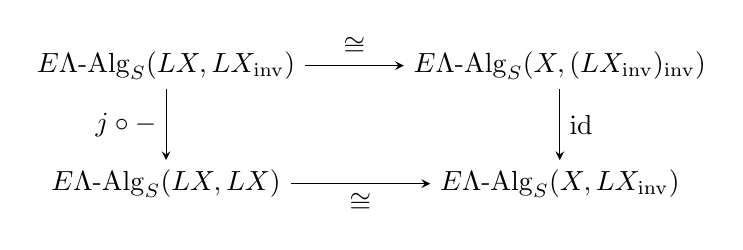
\begin{tikzpicture}[x=50mm,y=15mm]
		\node (a) at (0,0) {$E\Lambda\mbox{-}\mathrm{Alg}_S(LX , LX_{\mathrm{inv}})$};
		\node (b) at (1,0) {$E\Lambda\mbox{-}\mathrm{Alg}_S(X, (LX_{\mathrm{inv}})_{\mathrm{inv}})$};
		\node (c) at (0,-1) {$ E\Lambda\mbox{-}\mathrm{Alg}_S(LX , LX)$};
		\node (d) at (1,-1) {$E\Lambda\mbox{-}\mathrm{Alg}_S(X, LX_{\mathrm{inv}})$};
			\draw [->] (a) to node [above] {$\cong$} (b);
			\draw [->] (b) to node [right] {$\id$} (d);
			\draw [->] (a) to node [left] {$j \circ -$} (c);
			\draw [->] (c) to node [below] {$\cong$} (d);
    \end{tikzpicture}
    \end{center}
in which the identity on the right is really $j_{\mathrm{inv}} \circ -$. Thus composition with $j$ is an isomorphism in this case, so the identity map on $LX$ factors as $j \circ g$ for some $g \colon  LX \rightarrow (LX)_{\mathrm{inv}}$. Since $j$ is an inclusion, this factorization forces it to be the identity.
\end{proof}

\begin{cor} \label{epi} The component of the unit of the adjunction $L \dashv (-)_{\mathrm{inv}}$ at $E\Lambda(\underline{n})$,  $\eta_{E\Lambda(\underline{n})} \colon  E\Lambda(\underline{n}) \rightarrow (L_n)_{\mathrm{inv}}$, is an epimorphism in $E\Lambda\mbox{-}\mathrm{Alg}_S$.
\end{cor}
\begin{proof}
By \cref{linveql}, we first have that $(L_n)_{\mathrm{inv}} = L_n$. Let $F,G \colon  L_n \rightarrow X$ be a pair of algebra maps for which $F \eta = G \eta$. Thus the algebra maps $E\Lambda(\underline{n}) \rightarrow X_{\mathrm{inv}}$ corresponding to $F, G$ are equal, so $F,G$ are equal.
\end{proof}

%\begin{rem}
%include forward ref to where we use \cref{epi}
%\end{rem}
%I couldn't find one





\section{Adjunctions involving monoidal categories}

This section will study three different adjunctions between $\ML$-monoidal categories\index{monoidal category!$\ML$-monoidal} on the one hand and categories such as that of monoids or commutative monoids on the other hand. Two of these adjunctions are purely formal, and are induced by adjunctions between categories and sets, while the third requires a direct proof. We then investigate some simple consequences of these adjunctions for $\ML$-monoidal categories of the form $L_n$.


Recall from \cref{symmoncor} that
the functor $\ob$ from categories to sets, taking the set of objects, is left adjoint to the functor $E$ of \cref{Defi:e_b}. This adjunction is monoidal, hence induces an adjunction $\ob \dashv E$ between $\lmc$ and $\mon$\nomenclature[C]{$\mon$}{of monoids and monoid homomorphisms}.
We also note that $\ob(\EL) = \Lambda$ as a $\ML$-operad.

\begin{Defi}
Let $\ML$ be an action operad. Let $T_{\ML}$\nomenclature[N]{$T_{\ML}$}{the terminal $\ML$-operad} denote the terminal $\ML$-operad in sets, which is a singleton set in each dimension with the unique action of $\Lambda_n$.
\end{Defi}

\begin{lem}
The category of algebras for $T_{\ML}$ is either the category of monoids, when $\ML$ is not crossed, or the category of commutative monoids, when $\ML$ is crossed.
\end{lem}
\begin{proof}
In the case that $\ML$ is not crossed, $\Lambda(n)$ acts on $X^n$ trivially so the free $T_{\ML}$-algebra monad coincides with the free monoid monad. When $\ML$ is crossed, $\Lambda(n)$ acts on $X^n$ via the surjection to $\Sigma_n$ so the free $T_{\ML}$-algebra monad coincides with the free commutative monoid monad.
\end{proof}

\begin{nota}
We write $D$ for the discrete category functor $\sets \rightarrow \cat$.
\end{nota}

\begin{prop}\label{pi0-D_adj}
The functor $\pi_0$ from categories to sets, taking the set of path components, is left adjoint to  $D$. This adjunction is monoidal, hence induces an adjunction between $\lmc$ and $T_{\ML}\mbox{-}\textrm{Alg}$.
\end{prop}
\begin{proof}
This is now a simple application of \cref{monoidaladj_cor}, where we now only note that the unit $1 \Rightarrow \pi_0 \circ D$ is the identity transformation.
\end{proof}



\begin{Defi} For a monoid $M$, we write $M^{\mathrm{gp}}$ for its \emph{group completion}\index{group completion}, the universal group with a homomorphism $M \rightarrow M^{\mathrm{gp}}$.  We write the functor $M \mapsto M^{\mathrm{gp}}$ as $\mathrm{gp}$.
\end{Defi}

\begin{rem}
The category of groups is a reflective subcategory of the category of monoids, and $\mathrm{gp}$ is the reflection.
\end{rem}

\begin{prop}\label{oblel_fg}
The functor $\ob \circ L \circ \EL \colon  \sets \rightarrow \mon$ is naturally isomorphic to the composite of the free group functor and the inclusion of groups into monoids.
\end{prop}
\begin{proof}
Using that the objects of $\EL(M)_{\mathrm{inv}}$ for a monoid $M$ are the same as the objects of $\EL(M^{\times})$, where $M^{\times}$ is the subgroup of invertible elements of $M$, we see that both of these functors are left adjoints to the functor $M \mapsto M^{\times}$.
\end{proof}
There are several different ways to calculate the group completion of a monoid. One is to use that fact that $M^{\mathrm{gp}}$ is the group whose group presentation is the same as the monoid presentation of $M$. That is, if $M$ is the quotient of the free monoid on generators $\mathcal{G}$ by the relations $\mathcal{R}$, then $M^{\mathrm{gp}}$ is the quotient of the free \emph{group} on generators $\mathcal{G}$ by relations $\mathcal{R}$. This makes finding the completion of free monoids particularly simple.

\begin{nota}
We write $M^{*n}$\nomenclature[N]{$M^{*n}$}{the coproduct of $n$ copies of the monoid $M$} for the coproduct of $n$ copies of the monoid $M$. We use the same notation for groups, although the $n$-fold coproduct of a group is different when considered as a monoid than as a group; it should be clear from context which we intend.
\end{nota}

\begin{cor}\label{Zobj}
The object monoid of $L_n$ is $\mathbb{Z}^{*n}$\nomenclature[N]{$\mathbb{Z}$}{the set of integers}, the group completion of the object monoid of $\ELn$. The restriction of $\eta$ (see \cref{eta}) on objects, $\mathrm{Ob}(\eta)$, is then the obvious inclusion $\mathbb{N}^{*n} \hookrightarrow \mathbb{Z}^{*n}$.
\end{cor}

The core of \cref{Zobj} --- that $\mathrm{Ob}(L_n)$ is the group completion of the monoid $\mathrm{Ob}(\ELn)$ --- makes concrete the sense in which the functor $L$ represents `freely adding inverses' to objects. Extending this same logic to connected components as well, it would seem reasonable to expect that $\pi_0(L_n)$ is also the group completion of $\pi_0(\ELn)$. This is indeed the case, and the proof proceeds analogously. We record this observation below. 

\begin{prop}\label{pilel_gppiel}
The functor $\pi_0 \circ L \colon  \lmc \rightarrow T_{\ML}\mbox{-}\mb{Alg}$ is naturally isomorphic to the functor $\mathrm{gp} \circ \pi_0$.
\end{prop}

\begin{cor}\label{Zconcomp} The connected components of $L_n$ are the group completion of the connected components of $\ELn$. Also, the restriction of $\eta$ onto connected components, $\pi_0(\eta)$, is the canonical map $\pi_0(\ELn) \rightarrow \pi_0(\ELn)^{\mathrm{gp}}$ associated with that group completion.
\end{cor}

We summarize these results below.
\begin{cor}\label{crossconcomp} If $G$ is a crossed action operad\index{action operad!crossed} then
\begin{itemize} 
\item the connected components of $L_n$ are the monoid $\mathbb{Z}^n$,
\item the restriction of $\eta$ to components is the obvious inclusion $\mathbb{N}^n \hookrightarrow \mathbb{Z}^n$, and
\item the assignment of objects to their component is given by the quotient map of abelianization $\mathrm{ab} \colon  \mathbb{Z}^{\ast n} \rightarrow \mathbb{Z}^n$.
\end{itemize}
If instead $G$ is non-crossed, then
\begin{itemize} \itemsep0em
\item the connected components of $L_n$ are the monoid $\mathbb{Z}^{\ast n}$,
\item the restriction of $\eta$ to components is the obvious inclusion $\mathbb{N}^{\ast n} \hookrightarrow \mathbb{Z}^{\ast n}$, and
\item the assignment of objects to their component is $\id_{\mathbb{Z}^{\ast n}}$.
\end{itemize}
\end{cor}

We now turn to our third adjunction, which is of a less formal nature than the first two. Recall that, using \cref{tenscomp}, that composition along invertible objects in $X$ can always be restated in terms of the tensor product. Thus in cases where every object of $X$ is invertible, the monoidal structure together with knowledge of each morphism's source and target will be enough to determine $X$ uniquely. Since all objects in $L_n$ are invertible, this means that we could choose to ignore composition of elements of $\MorLn$ for the time being, and focus on its status as a monoid under tensor product.



\begin{Defi}\label{def:M} Let $\mathrm{M} \colon \moncat \rightarrow \mon$ be the functor which sends a monoidal category $X$ to the quotient of its monoid of morphisms\index{monoidal category!monoid of morphisms} by the relation that sets $\otimes = \circ$. :
  \[
    \mathrm{M}X \quad = \quad \bigquotient{\mathrm{Mor}(X)}{f' \circ f \sim f' \otimes f}.
  \]
If $F \colon X \rightarrow Y$ is a strict monoidal functor, then $MF$ is the monoid homomorphism sending the class of a morphism $g$ to the class of $Fg$; the reader will easily check this is well-defined. We will call $\mathrm{M}X$ the \emph{collapsed} morphisms of $X$.
\end{Defi}

\begin{nota}
If $f$ is a morphism in $X$, we write its class in $\mathrm{M}X$ as $\mathrm{M}f$, and we write the single operation $\otimes$ rather than $\circ$. Note that the class $\mathrm{M}(f') \otimes \mathrm{M}(f)$ always contains $f' \otimes f$, but will only contain $f' \circ f$ if this latter morphism exists.
\end{nota}


Now we need a candidate for the right adjoint to the functor $\mathrm{M}$.

\begin{Defi} 
Let $B \colon  \mon \rightarrow \cat$ denote the functor sending a monoid $M$ to the one-object category whose single hom-set consists of the elements of $M$, with composition and identity being given by multiplication and the unit of $M$, respectively. We also denote by $B$ the functor $\cmon \rightarrow \moncat$\nomenclature[C]{$\cmon$}{of commutative monoids and monoid homomorphisms} the functor sending a commutative monoid $A$ to the same category $BA$, now equipped with the monoidal structure which is trivial on the single object and $a \otimes b = a \circ b = ab$ on morphisms (writing the monoid operation in $A$ as concatenation here).
\end{Defi}




Note that for any monoidal category $M$, the monoid $M(I,I)$ is always commutative by the Eckmann-Hilton argument \cite{eh, cg-periodic2}, hence the requirement of commutativity to lift $B$ to a functor into monoidal categories.




\begin{Defi} For a monoid $M$, we write $M^{\mathrm{ab}}$ for its \emph{abelianization}\index{abelianization}, the universal commutative monoid with a homomorphism $M \rightarrow M^{\mathrm{ab}}$.  We write the functor $M \mapsto M^{\mathrm{ab}}$ as $\mathrm{ab}$. We use the same notation for groups as well.
\end{Defi}

\begin{rem}
The categories of commutative monoids, resp. abelian groups, are reflective subcategories of the categories of monoids, resp. groups, and $\mathrm{ab}$ is the reflection.
\end{rem}


\begin{prop}\label{Moradj} $\mathrm{B} \colon  \cmon \rightarrow \moncat$ is a right adjoint to the functor $\mathrm{M}(\, - \,)^{\mathrm{ab}} \colon \moncat \rightarrow \cmon$.
\end{prop}
\begin{proof}
For a commutative monoid $A$, it is clear that $M(BA)^{\mathrm{ab}} = A$, so we can define the counit to be the identity. For a monoidal category $X$, define $X \rightarrow B(MX^{\mathrm{ab}})$ by sending every object of $X$ to the unique object, and by sending the morphism $f$ to the morphism given by the equivalence class of $f$. This is clearly natural in strict monoidal functors $X \rightarrow Y$, and the triangle identities make for a straightforward calculation.

\end{proof}

\cref{Moradj} seems at first glance very similar to \cref{Obadj,concompadj}. However, our goal was to discover the relationship between the morphisms of $\ELn$ and $L_n$, paralleling what we did in \cref{Zobj,Zconcomp}, and in that regard $\mathrm{M}$ falls short in two very important ways. 

\begin{enumerate}
\item Our goal was to have an adjunction involving $\lmc$, not $\moncat$, since we want to apply it to strict $\ML$-monoidal functors instead of arbitrary strict monoidal functors. 
\item Even if we do find a way to use this adjunction to extract information about $L_n$, it will not be the monoid $\MorLn$ we were originally after, only a strange abelianized version where tensor product and composition coincide.  
\end{enumerate} 

Unfortunately, this adjunction seems to be the best that we can do. 
\begin{prop}
The functor $B \colon \cmon \rightarrow \moncat$ lifts to a functor $B \colon \cmon \rightarrow \lmc$. This functor $B$ has a left adjoint $M' \colon \lmc \rightarrow \cmon$, but both functors
  \[
    M' \circ \EL, \, M' \circ L \circ \EL \colon \sets \rightarrow \cmon
  \]
are isomorphic to the functor sending every set to the trivial commutative monoid.
\end{prop}
\begin{proof}
To lift $B$ to $\lmc$, we need only assign the trivial action of each $\Lambda_n$. The existence of $M'$ is guaranteed by the adjoint functor theorem for locally finitely presentable categories since $B$ clearly preserves limits and filtered colimits.  For a set $S$ and commutative monoid $A$, monoid homomorphisms $M' \circ \EL(S) \rightarrow A$ are in bijection with strict $\ML$-monoidal functors $\EL(S) \rightarrow BA$ which are themselves in bijection with functions $S \rightarrow \ob(BA) = *$, so there is a unique such monoid homomorphism, and $M' \circ \EL(S) \cong 0$ as commutative monoids. The same proof works for $M' \circ L \circ \EL$ after we note that $(BA)_{\mathrm{inv}} = BA$.
\end{proof}





 We will eventually prove that the morphisms of $L_n$ actually form a group under tensor product in \cref{tensinv}, so instead of working directly with the functor $\mathrm{M}(\, - \,)^{\mathrm{ab}} \colon  \moncat \rightarrow \cmon$, we will focus on its composite with the group completion functor, $\mathrm{gp} \colon \cmon \rightarrow \mb{Ab}$. We end with a brief exploration of this new functor $\mathrm{M}(\, - \,)^{\mathrm{gp},\mathrm{ab}}$.  
It is well known that group completion and abelianization commute since their right adjoints commute, but we further note that group completion commutes with collapsing morphisms.


\begin{lem}\label{Morder} For any monoidal category $X$, define
  \begin{align*}
  		\mathrm{M}_{\mathrm{gp}}(X) &= \bigquotient{\mathrm{Mor}(X)^{\mathrm{gp}}}{\mathrm{gp}(f' \circ f) \sim \mathrm{gp}(f' \otimes f)},\\
  		\mathrm{M}_{\mathrm{ab}}(X) &= \bigquotient{\mathrm{Mor}(X)^{\mathrm{ab}}}{\mathrm{ab}(f' \circ f) \sim \mathrm{ab}(f' \otimes f)}.
  \end{align*}

Then
  \begin{align*}
    \mathrm{M}_{\mathrm{gp}}(X) \cong \mathrm{M}(X)^{\mathrm{gp}},\\
    \mathrm{M}_{\mathrm{ab}}(X) \cong \mathrm{M}(X)^{\mathrm{ab}}.
  \end{align*}
\end{lem}
\begin{proof}
This follows immediately from $M$ being given explicitly as a quotient, and both functors $\mathrm{ab}$ and $\mathrm{gp}$ preserving colimits..
\end{proof}


QQQ Institute the following where possible
\begin{conv}\label{plus}
We default to writing any abelian group, such as those in the image of $\mathrm{M}(\, - \,)^{\mathrm{gp},\mathrm{ab}}$, with additive notation, using $+$ for the group operation and 0 for the identity element.
\end{conv}



\section{The free object as a cokernel}
\label{colimalgebra} 
This section will present a different approach to $L_n$. Consider for a moment the free $\ML$-monoidal category on $2n$ objects $z_1, z_2, \ldots, z_{2n}$. If we were to take this category and then add the relations $z_{n+1} = z_1^{-1}, \ldots, z_{2n} = z_n^{-1}$, then we would be changing it from a structure with $2n$ independent generators into one with $n$ independent generators and their inverses. Thus we would see $L_n$ as a quotient of the larger monoidal category $\EL(2n)$. We will now work towards making this idea precise, and then examine some of its consequences, the most important of which will be allowing us to describe the group $\MLn^{\mathrm{gp},\mathrm{ab}}$.





\begin{Defi}\label{qdef} Let $\delta \colon \EL(\underline{2n})\rightarrow \EL(\underline{2n})$ be the map of $\ML$-monoidal categories defined on generators by
  \begin{align*}
  		\delta(z_{i}) &= z_i \otimes z_{n+i}, \\
  		\delta(z_{n+i}) &= z_{n+i} \otimes z_i
  \end{align*}
for $1 \le i \le n$. We will also denote by $q \colon  \EL(\underline{2n}) \rightarrow Q$ the cokernel of this map (i.e., the coequalizer of this functor and the functor sending all objects to the unit and all morphisms to the identity).  
\end{Defi}


The first goal of this section is to show that $Q \cong L_n$.

\begin{prop}\label{Qobj} The object monoid of $Q$ is $\mathbb{Z}^{*n}$, and the restriction of $q$ to objects $\mathrm{Ob}(q) \colon  \mathrm{Ob}(\ELnn) \rightarrow \mathrm{Ob}(Q)$ is the monoid homomorphism
  \[
    \mathrm{Ob}(q) \colon \mathbb{N}^{\ast 2n} \rightarrow \mathbb{Z}^{\ast n}
  \]
defined on generators by:
  \begin{align*}
  			\mathrm{Ob}(q)(z_i) &= z_i,\\
  			\mathrm{Ob}(q)(z_{n+i}) &= z_i^*.		
  \end{align*}
\end{prop}
\begin{proof}
Since $\ob$ is a left adjoint, it preserves colimits and thus cokernels. It is clear, from the presentation, that the cokernel on objects is $\ZZ^{*n}$.
\end{proof}


\begin{prop}\label{coker} Let $i \colon  \ELn \rightarrow \EL(\underline{2n})$ be the inclusion of $\ML$-monoidal categories defined on generators by $i(z_j) = z_j$. Then $qi$ exhibits $Q$ as the initial $\ML$-monoidal category on $n$ invertible objects, so $Q \cong L_n$.
\end{prop}
\begin{proof}
\cref{Qobj} gives a unique map shown by the dashed arrow below.
    \[
  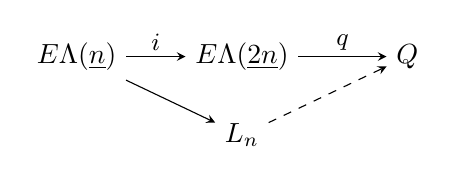
\begin{tikzpicture}[x=7mm,y=5mm]
    \draw[tikzob,mm] 
    (0,0) node (0) {\EL(\underline{n})}
    (3,0) node (1) {\EL(\underline{2n})}
    (6,0) node (2) {Q}
    (3,-2) node (d) {L_n};
    \path[tikzar,mm] 
    (0) edge node {i} (1)
    (1) edge node {q} (2)
    (0) edge (d)
    (d) edge[dashed] (2);
  \end{tikzpicture}
  \]
We also have a unique map $\EL(\underline{2n}) \rightarrow L_n$ which agrees with the canonical map $\EL(\underline{n}) \rightarrow L_n$ on $z_1, \ldots, z_n$ and sends $z_{i+n}$ to the inverse of the image of $z_i$. This gives the diagram below, once again with the dashed arrow induced by the definition of $\delta$ and the universal property.
    \[
  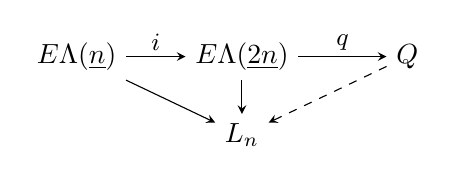
\begin{tikzpicture}[x=7mm,y=5mm]
    \draw[tikzob,mm] 
    (0,0) node (0) {\EL(\underline{n})}
    (3,0) node (1) {\EL(\underline{2n})}
    (6,0) node (2) {Q}
    (3,-2) node (d) {L_n};
    \path[tikzar,mm] 
    (0) edge node {i} (1)
    (1) edge node {q} (2)
    (0) edge (d)
    (1) edge (d)
    (2) edge[dashed] (d);
  \end{tikzpicture}
  \]
 The two dashed arrows are then forced to be inverse to each other. 
\end{proof}


\begin{Defi}
We will say that a functor $F \colon  C \rightarrow D$ is \emph{surjective}\index{functor!surjective} if the underlying map of graphs is surjective. In particular $F$ must be surjective on objects, but it need not be full.
\end{Defi}

\begin{prop}\label{coeqsurj} Let $\phi, \phi' \colon X \rightarrow Y$ be a pair of $E\Lambda$-algebra maps, and $k \colon  Y \rightarrow Z$ their coequalizer in $E\Lambda\mbox{-}\mathrm{Alg}_S$. If the monoid $\mathrm{Ob}(Z)$ is also a group, then the functor $k$ is surjective.
\end{prop}
\begin{proof}
Since the functor $\mathrm{Ob} \colon E\Lambda\mbox{-}\mathrm{Alg}_S \rightarrow \mon$ is a left adjoint, it preserves all colimits so the monoid homomorphism $\mathrm{Ob}(k) \colon  \mathrm{Ob}(Y) \rightarrow \mathrm{Ob}(Z)$ is the coequalizer of the parallel pair $\mathrm{Ob}(\phi), \mathrm{Ob}(\phi')$ in the category of monoids. Every coequalizer is a regular epimorphism, and in the category of monoids regular epimorphisms coincide with  surjective functions, so $k$ is surjective on objects.


Next, let $f \colon  v \rightarrow w$ and $f' \colon w' \rightarrow v'$ be any two morphisms of the category $Y$ for which $k(f)$ and $k(f')$ are composable in $Z$. Since these maps are composable we know that $k(w)$ and $k(w')$ must be the same object of $Z$, and since $\mathrm{Ob}(Z)$ is a group we know this object has an inverse $k(w)^{-1} = k(w')^{-1}$. So by the surjectivity of $k$ we can find another object $y$ of $Y$ for which $k(y) = k(w)^{-1}$. Using this, define the morphism $h \colon  w' \otimes y \otimes v \rightarrow v' \otimes y \otimes w$ to be the tensor product $f' \otimes \id_y \otimes f$. Thus
  \begin{align*}
  	k(h) & = & k(f' \otimes \id_y \otimes f) \\
  	& = & k(f') \otimes \id_{k(y)} \otimes k(f) \\
  	& = & k(f') \otimes \id_{k(w)^{-1}} \otimes k(f)
  \end{align*}
and so by \cref{tenscomp}, this is the composite $k(f') \circ k(f)$. Therefore the set of morphisms of $Z$ which are images of morphisms of $Y$ is closed under composition. 

Now consider $k(Y)$, the subcategory of $Z$ that contains every object $x'$ for which there exists $x$ in $Y$ with $k(x) = x'$, and every morphism $f'$ for which there exists $f$ in $Y$ with $q(f) = f'$. We know that the morphisms of $k(Y)$ are closed under composition, and so this is indeed a well-defined category. It is easy to see that $k(Y)$ is in fact a well-defined sub-$\ML$-monoidal category, and that $k' \colon  Y \rightarrow k(Y)$ is a surjective strict $\ML$-monoidal functor. This shows that $k'$ coequalizes $\phi, \phi'$, so the inclusion $k(Y) \hookrightarrow Z$ must be an isomorphism and thus $k$ is surjective.
\end{proof}

\begin{rem}\label{alsowithoutgroups}
Note that, since no feature of $\ML$ is used in the above proofs, they all apply equally in the case of no group actions at all, i.e., for strict monoidal categories or when $\ML = \mb{T}$ is the terminal action operad consisting only of trivial groups.
\end{rem}

\begin{cor}\label{qsurj} The cokernel map $q \colon  \EL(\underline{2n}) \rightarrow L_n$ is surjective.
\end{cor}

\begin{cor}\label{M_coker}
There is an isomorphism of groups as below.
  \[
    \MLn^{\mathrm{gp},\mathrm{ab}} \quad \cong \quad \bigquotient{\mathrm{M}(\ELnn)^{\mathrm{gp},\mathrm{ab}}}{\mathrm{ker}\left( \, \mathrm{M}(q)^{\mathrm{gp},\mathrm{ab}} \, \right)}
  \]
\end{cor}

One important consequence of the surjectivity of $q$ is that it will allow us to use some results about the free algebra $\ELnn$ to deduce information about the free invertible algebra $L_n$. In fact, we have done this once already: looking back at \cref{Qobj} with our current knowledge that $Q = L_n$, we can see that it is a direct analogue of \cref{Gnobj}, using the fact that $q$ is surjective on objects. 

In that same vein, one might ask if we can take \cref{hom-set-lemma}, a statement about the morphisms in free $\ML$-monoidal categories, and extend it to an analagous result on $L_n$, using surjectivity of $q$ on morphisms instead. 

\begin{nota}\label{newaction}
Let's think about $g^{\otimes}$ for the iso induced by $g$.
\end{nota}

\begin{lem}\label{otimesotimes}
Later I use: $(h \otimes g)^{\otimes} = h^{\otimes} \otimes g^{\otimes}$.
\end{lem}

\begin{prop} \label{allmapsaction} Every morphism in $L_n$ can be expressed as $g^{\otimes}$
for some $g \in \Lambda(m)$ and $x_i \in \{z_1, \ldots, z_n, z_1^*, \ldots, z_n^* \}$.
\end{prop}

\begin{proof}
Let $f$ be an arbitrary morphism in $L_n$. By surjectivity of $q$, there must exist at least one morphism $f'$ in $\ELnn$ such that $q(f') = f$, and from \cref{hom-set-lemma} we know that this $f'$ can be expressed uniquely as $g^{\otimes}$ for some $g \in \Lambda(m)$. 
\end{proof}

Note that while this result shows that every morphism of $L_n$ is induced by the action of some $g \in \Lambda(m)$, it does not imply that this $g$ is unique.

\begin{conv}
The monoid homomorphism $\mathrm{Ob}(q)  \colon  \mathbb{N}^{\ast 2n}  \rightarrow  \mathbb{Z}^{\ast n}$ has a canonical section $q^{-1}$ given as follows. An element $w \in \mathbb{Z}^{* n}$ can be written as a word in $z_i, z_i^*$ in normal form, that is in the fewest number of symbols with instances of $z_i$ or $z_i^*$ appearing before those of $z_j, z_j^*$ when $i < j$. We define $q^{-1}(z_i) = z_i$ and $q^{-1}(z_i^*) = z_{n+i}$, and then 
  \[
    q^{-1}(w) = q^{-1}(w_1) \cdots q^{-1}(w_k)
  \]
where $w = w_1 \cdots w_k$ is the normal form of $w$. We note that $q^{-1}$ is merely a function, and not a monoid homomorphism.
\end{conv}

\begin{cor}\label{action_on_L}
For $g \in \Lambda(m)$ and $x_1, \ldots, x_m$ objects of $L_n$, the isomorphism
  \[
    g^{\otimes} \colon  a_1 \otimes \cdots \otimes a_m \rightarrow a_{\pi(g)^{-1}(1)} \otimes \cdots \otimes a_{\pi(g)^{-1}(m)}
  \]
is
%QQQ Is this the right notation?
\[
q \left(g^{\otimes} \colon  q^{-1}(a_1) \otimes \cdots \otimes q^{-1}(a_m) \rightarrow   q^{-1}(a_{\pi(g)^{-1}(1)}) \otimes \cdots \otimes q^{-1}(a_{\pi(g)^{-1}(m)})    \right).
\]
\end{cor}

\section{A second coequalizer argument}
In this section, we will compare the coequalizer of a diagram of $\ML$-monoidal categories as it is computed in $\lmc$, in $\moncat$, and in $\cat$. Our goal will be to show that the forgetful functors 
  \[
    \lmc \rightarrow \moncat \rightarrow \cat
  \]
all create reflexive coequalizers. This has the effect of allowing us to compute coequalizers in $\lmc$ by converting them into reflexive coequalizers and then computing them in either $\moncat$ or $\cat$. This technique will be necessary in our construction of the free $\ML$-monoidal category on $n$ invertible objects. The strategy here follows that in Section 4.1 of \cite{lack-cod}.

\begin{lem}\label{P_pres_refl}
Let $P$ be a $\ML$-operad in $\cat$, with $\und{P}$ its associated 2-monad. Then $\und{P}$ preserves reflexive coequalizers.

\end{lem}
\begin{proof}
We have a functor $P \colon B\ML^{op} \rightarrow \cat$ which sends $n$ to $P(n)$ and uses the right action $P(n) \times \ML(n) \rightarrow P(n)$ to define the functor on morphisms. Given a category $X \in \cat$, there is also a functor $R_X \colon B\ML \rightarrow \cat$ sending $n$ to $X^n$ and $g \in \Lambda(n)$ to the permutation given by $\pi(n)$. The weighted colimit $P \cdot R_X$ is then easily seen to be the free algebra $\und{P}(X)$. The functor $P \cdot -$ is cocontinuous, so the free $\und{P}$-algebra functor $\cat \rightarrow \cat$ will preserve whatever colimits the functor $X \mapsto R_X$ preserves. Colimits in the functor category $[B\ML, \cat]$ are computed pointwise, and the functors $X \mapsto X^n$ for $n \in \mathbb{N}$ preserve reflexive coequalizers, so $X \mapsto R_X$ does also and therefore the free $\und{P}$-algebra functor preserves reflexive coequalizers.
\end{proof}

\begin{lem}\label{creation_triangle}
Let $A,B,C$ be cocomplete categories, and let $A \stackrel{F}{\to} B \stackrel{G}{\to} C$ be functors such that $G$ is conservative, and both $G$ preserves and $GF$ creates colimits of shape $\mathbb{D}$. Then $F$ creates colimits of shape $\mathbb{D}$.
\end{lem}

For an monad $T$ on a category $C$, the forgetful functor $T\Alg \rightarrow C$ creates any colimit that $T$ preserves. This fact and the previous lemmas prove the following proposition using the operad $P = E\ML$.
\begin{prop}\label{refcoeq_calcs}
For any action operad $\ML$, the forgetful functor $\ML\mbox{-}\moncat \rightarrow \cat$ is conservative and creates reflexive coequalizers. Consequently, $\ML\mbox{-}\moncat \rightarrow \moncat$ is also conservative and creates reflexive coequalizers.

\end{prop}

\begin{nota}\label{plus_notation}
Let $f \colon  A \rightarrow C, g \colon  B \rightarrow C$ be maps in a category with coproducts. We will write $f;g \colon  A \coprod B \rightarrow C$ for the unique map induced by the universal property of the coproduct.
\end{nota}

\begin{lem}\label{sum_coeq}
Let $f, g \colon  A \rightarrow B$ be maps in a cocomplete category with coequalizer $c \colon  B \rightarrow C$. Then $c$ is also the coequalizer of $f;\id_B$ and $g; \id_B$, and this expresses $c$ as a reflexive coequalizer.
\end{lem}
\begin{proof}
A map $h \colon  B \rightarrow X$ coequalizes $f;\id_B$ and $g; \id_B$ if and only if $hf = hg$ and $h \id_B = h \id_B$ by the universal property of the coproduct, so $c$ is still the universal map which coequalizes. Reflexivity is easy, as the canonical inclusion map $B \rightarrow A \coprod B$ is a common section.

\end{proof}

\begin{Defi} \label{coprodmapdef} Let $\tilde{\delta} = \id_{\ELnn};\delta$.
Explicitly, $\tilde{\delta} \colon \ELnnnn \rightarrow \ELnn$ is the map of $E\Lambda$-algebras which acts on generators by
  \begin{align*}
		% \tilde{\delta} & \colon & \ELnnnn & \rightarrow & \ELnn \\
		\tilde{\delta}(z_i) &= z_i, \\
		\tilde{\delta}(z_{n+i}) &= z_{n+i}, \\
		\tilde{\delta}(z_{2n+i}) &= z_i \otimes z_{n+i}, \\
		\tilde{\delta}(z_{3n+i}) &= z_{n+i} \otimes z_i
	\end{align*}
for $1 \le i \le n$. Similarly, let $\tilde{I} = \id_{\ELnn};I$.
Explicitly, $\tilde{I} \colon \ELnnnn \rightarrow \ELnn$ is the map of $E\Lambda$-algebras which acts on generators by
  \begin{align*}
		% \tilde{I} & \colon & \ELnnnn & \rightarrow & \ELnn \\
		\tilde{I}(z_i) &= z_i,  \\
		\tilde{I}(z_{n+i}) &= z_{n+i}, \\
		\tilde{I}(z_{2n+i}) &= I, \\
		\tilde{I}(z_{3n+i}) &= I
	\end{align*} 
for $1 \le i \le n$. 
\end{Defi}



\begin{cor}\label{q_other_coeq} The functor $q$ (\cref{qdef}) is the coequalizer of $\tilde{\delta}$ and $\tilde{I}$ in $\ELAlg$.
\end{cor}

By construction, $\tilde{\delta}$ and $\tilde{I}$ form a reflexive pair in $\ELAlg$, so by \cref{refcoeq_calcs} we have the further corollary below.

\begin{cor}\label{q_other_coeq2} The functor $q$  is the coequalizer of $\tilde{\delta}$ and $\tilde{I}$ in $\moncat$ or in $\cat$.
\end{cor}


\section{From strictly to weakly invertible objects}

We now turn to weakly invertible objects, and more specifically how we can apply our results about invertible objects to the weakly invertible ones. We begin with the analogue of \cref{invdef}.

\begin{Defi}\label{winvdef}
Given an $E\Lambda$-algebra $X$, we will denote by $X_{\mathrm{winv}}$\nomenclature[N]{$X_{\mathrm{inv}}$}{the sub-$E\Lambda$-algebra of $X$ of objects weakly invertible under tensor product}\index{algebra!of weakly invertible objects} the sub-$E\Lambda$-algebra of $X$ containing all objects which are weakly invertible under tensor product, and all of the isomorphisms between them.
\end{Defi}

We have analogues of the following propositions, the proofs of which are, \textit{mutatis mutandis}, the same as for invertible objects.

\begin{prop} \label{winvprop} The assignment $X \mapsto X_{\mathrm{winv}}$ can be extended to a 2-functor $(\_)_{\mathrm{winv}} \colon  \ELAlg \rightarrow \ELAlg$.
\end{prop}

\begin{prop} \label{winvadj} The 2-functor $(\_)_{\mathrm{inv}} \colon  \ELAlg \rightarrow \ELAlg$ has a left adjoint, $K \colon  \ELAlg \rightarrow \ELAlg$.
\end{prop}

\begin{Defi}\label{kn}
Let $K_n$ denote the free $\ML$-monoidal category generated by $n$ weakly invertible objects.
\end{Defi}


\begin{thm}\label{L_is_K}
The canonical $\ML$-monoidal functor $\tau \colon K_n \rightarrow L_n$ is an equivalence of $\ML$-monoidal categories.
\end{thm}
\begin{proof}
QQQ
Reduce to the case $n=1$ using some coproducts

Prove a weakly invertible object is the same a strong $\ML$-monoidal functor $L_1 \rightarrow X$

Use some coherence theorems
\end{proof}

\chapter{Invertibility and group actions}
The goal of this chapter is to reduce coherence questions about invertible objects (be they strict or weak by \cref{L_is_K}) to the calculation of a group action. The group we are interested in is the group of automorphisms of the unit, $L_n(I,I)$, and it acts on $L_n(x,y)$ for any two objects $x$ and $y$. In \cref{splitting_as_coh}, we will explain how to use this group action to determine whether some pair of parallel morphisms are equal or not.

More intro here

\section{Sources and targets in \texorpdfstring{$L_n$}{L_n}}   

\begin{Defi}\label{st} For any $\ML$-monoidal category $X$, denote by $s \colon  \mathrm{Mor}(X) \rightarrow \mathrm{Ob}(X)$ and $t \colon  \mathrm{Mor}(X) \rightarrow \mathrm{Ob}(X)$ the monoid homomorphisms which send each morphism of $X$ to its source and target, respectively. That is,
  \begin{align*}
    s(f \colon  x \rightarrow y) &= x,\\
    \quad \quad t(f \colon  x \rightarrow y) &= y.
  \end{align*}
\end{Defi}

\begin{Defi}\label{s_times_t}
For a $\ML$-monoidal category $X$, define $(s \times t)(X)$ to be the pullback (in the category of monoids) $\mathrm{Ob}(X) \times_{\pi_0(X)} \mathrm{Ob}(X)$ of the diagram below. 
\[ \begin{tikzcd}
\mathrm{Ob}(X) \times_{\pi_0(X)} \mathrm{Ob}(X) \ar[dd, shift left=12] \ar[rr] \ar[ddrr, phantom, "\lrcorner", near start, shift left=4] & & \mathrm{Ob}(X) \ar[dd, "\lbrack \, \_ \, \rbrack"] & \\ 
& & & \\
\quad \quad \quad \quad \quad \quad \mathrm{Ob}(X) \ar[rr, "\lbrack \, \_ \, \rbrack"] & & \pi_0(X)
\end{tikzcd} \]
\end{Defi}

\begin{lem}\label{stmon} Let $X$ be a $\ML$-monoidal category whose underlying category is a groupoid, and $s \times t \colon  \mathrm{Mor}(X) \rightarrow \mathrm{Ob}(X)^2$ the map induced from $s$ and $t$ using the universal property of products. Then the image of this map is $(s \times t)(X)$.
\end{lem} 


Recalling \cref{Gnobj,Gnconcomp,Zobj,crossconcomp}, we can immediately conclude the following.

\begin{cor} \label{stpullback}
  \[
    \begin{array}{rll} 
  		(s \times t)(\ELn) & \cong & \begin{cases}
  								\quad \mathbb{N}^{\ast n} \times_{\mathbb{N}^n} \mathbb{N}^{\ast n} & \text{if $G$ is crossed}\\
  								\quad \mathbb{N}^{\ast n} & \text{otherwise}
  							\end{cases} \\
  		& & \\
  		(s \times t)(L_n) & \cong & \begin{cases}
  								\quad \mathbb{Z}^{\ast n} \times_{\mathbb{Z}^n} \mathbb{Z}^{\ast n}  & \text{if $G$ is crossed}\\
  								\quad \mathbb{Z}^{\ast n} & \text{otherwise}
  							\end{cases} \\
    \end{array}
  \]
where the pullbacks are taken over the quotients of abelianization for $(\mathbb{N}^{\ast n})^{\mathrm{ab}} = \mathbb{N}^n$ and $(\mathbb{Z}^{\ast n})^{\mathrm{ab}} = \mathbb{Z}^n$ respectively.
\end{cor}

Before continuing further, we establish some elementary properties of the monoid $\mathbb{N}^{\ast n} \times_{\mathbb{N}^n} \mathbb{N}^{\ast n}$ and the group $\mathbb{Z}^{\ast n} \times_{\mathbb{Z}^n} \mathbb{Z}^{\ast n}$.

\begin{Defi}\label{length}
Let $S$ be a set, and consider the free monoid $\N^{*S}$ given by words in the elements of $S$. \emph{Length} $\ell \colon \N^{*S} \rightarrow \N$ is the monoid homomorphism which is given by the identity homomorphism on each copy of $\N$ in the coproduct $\N^{*S}$. Concretely, the length $\ell(w)$ of a word $w \in \N^{*S}$ is the total number of letters in it.
\end{Defi}

\begin{lem}\label{freemon} $\mathbb{N}^{\ast n} \times_{\mathbb{N}^n} \mathbb{N}^{\ast n}$ is a free monoid.
\end{lem}
\begin{proof}
Write the generators for the first copy of $\mathbb{N}^{\ast n}$ in $\mathbb{N}^{\ast n} \times_{\mathbb{N}^n} \mathbb{N}^{\ast n}$ as $a_1, \ldots, a_n$, and the generators for the second copy of $\mathbb{N}^{\ast n}$ as $x_1, \ldots, x_n$. An element $(w,w') \in \mathbb{N}^{\ast n} \times_{\mathbb{N}^n} \mathbb{N}^{\ast n}$ can therefore be written uniquely as
  \[
    (w,w') = (a_{i_1} a_{i_2} \cdots a_{i_k}, x_{i_1} x_{i_2} \cdots x_{i_j})
  \]
and being an element of the pullback immediately implies $k=j$. We then define an element $ (a_{i_1} a_{i_2} \cdots a_{i_k}, x_{i_1} x_{i_2} \cdots x_{i_k})$ of $\mathbb{N}^{\ast n} \times_{\mathbb{N}^n} \mathbb{N}^{\ast n}$ to be indecomposable if there does not exist an $h < k$ such that $ (a_{i_1} a_{i_2} \cdots a_{i_h}, x_{i_1} x_{i_2} \cdots x_{i_h})$ is also an element of $\mathbb{N}^{\ast n} \times_{\mathbb{N}^n} \mathbb{N}^{\ast n}$. It is clear that every element can be written as a product of indecomposables. If $(w,w')$ can be written as a product of indecomposables in two ways, say 
  \[
    (w,w') = c_1 \cdots c_s = d_1 \cdots d_t,
  \]
then the length  of $c_1$ must be either strictly less than or strictly greater than the length of $d_1$; if they had equal length, then they would be equal. Without loss of generality assume $\ell(c_1) < \ell(d_1)$. But then the first $\ell(c_1)$ terms appearing in $d_1$ would agree with $c_1$, proving that $d_1$ is not indecomposable. Straightforward induction then finishes the proof that every element of $\mathbb{N}^{\ast n} \times_{\mathbb{N}^n} \mathbb{N}^{\ast n}$ can be written as a product of indecomposables in a unique way, making $\mathbb{N}^{\ast n} \times_{\mathbb{N}^n} \mathbb{N}^{\ast n}$ free on the set of indecomposables.
\end{proof}

Recall the $\ML$-monoidal functors $\delta \colon \ELnn \rightarrow \ELnn$ and $q \colon \ELnn \rightarrow L_n$. The construction $X \mapsto (s \times t)(X)$ is a functor $\lmc \rightarrow \mon$, so these induce monoid homomorphisms that we also write, by abuse of notation, as 
  \begin{align*}
    (\delta, \delta) \colon  \mathbb{N}^{\ast 2n} \times_{\mathbb{N}^{2n}} \mathbb{N}^{\ast 2n} &\rightarrow \mathbb{N}^{\ast 2n} \times_{\mathbb{N}^{2n}} \mathbb{N}^{\ast 2n}, \\
    (q, q) \colon  \mathbb{N}^{\ast 2n} \times_{\mathbb{N}^{2n}} \mathbb{N}^{\ast 2n} &\rightarrow \mathbb{Z}^{\ast n} \times_{\mathbb{Z}^n} \mathbb{Z}^{\ast n}. 
  \end{align*}

\begin{lem}\label{monoid_coeq}
The monoid homomorphism $(q,q)$ exhibits $\mathbb{Z}^{\ast n} \times_{\mathbb{Z}^n} \mathbb{Z}^{\ast n}$ as the cokernel of the monoid homomorphism $(\delta, \delta)$.
\end{lem}
\begin{proof}
QQQ I'm not sure this is correct, or if it is then it isn't obvious as claimed.
\end{proof}

\begin{lem}\label{rho_lemmas}
If $(w,w') \in \mathbb{N}^{\ast 2n} \times_{\mathbb{N}^{2n}} \mathbb{N}^{\ast 2n}$ is indecomposable, then so is $\delta(w,w')$. For any indecomposable $(w,w')$, there exists a unique natural number $k$ and indecomposable $(v,v')$ such that
  \[
    (w,w') = \delta^k(v,v')
  \]
but $(v,v')$ is not $\delta(u,u')$ for any indecomposable $(u,u')$.
\end{lem}
\begin{proof}
The first statement follows immediately from the injectivity of $\delta$ on objects, and the second from the fact that $\delta$ doubles the length of any element.
\end{proof}


We now want to show that the group $(s \times t)(L_n)$ we have described is in fact a submonoid of $\MorLn$.  We will accomplish this  by first proving the analogous statement for all $\ELn$.  For any pair $(w, w') \in \mathbb{N}^{\ast n} \times_{\mathbb{N}^n} \mathbb{N}^{\ast n}$ such that the images of $w$ and $w'$ in the commutative monoid $\mathbb{N}^n$ are the same, there are generators $x_1, \ldots, x_m$ for which 
  \[
    w = x_1 \otimes \ldots \otimes x_m
  \]
and there exists at least one permutation $\sigma \in \Sigma_m$ such that
  \[
    w' = x_{\sigma(1)} \otimes \ldots \otimes x_{\sigma(m)}.
  \]
Since the underlying permutation maps $\pi \colon \Lambda(m) \rightarrow \Sigma_m$ of a crossed action operad $\ML$ are all surjective, we can always find an element of $g \in \Lambda(m)$ for which $\pi(g) = \sigma$. 

\begin{nota}\label{rho_ww'}
Let $\rho \colon \mathbb{N}^{\ast n} \times_{\mathbb{N}^n} \mathbb{N}^{\ast n} \rightarrow \bigcup \EL(m)$ be an arbitrary, but fixed, function such that $\rho(w,w')$ satisfies $\pi(\rho(w,w')) = \sigma$ as defined above.
\end{nota}

We can now construct the desired injection using the function $\rho$ from \cref{rho_ww'}.
\begin{prop}\label{stGnsub} $\mathrm{Mor}(\ELn) \rightarrow (s \times t)(\ELn)$ is a split epi of monoids, so $(s \times t)(\ELn)$ is (isomorphic to) a submonoid of $\mathrm{Mor}(\ELn)$. Furthermore, we can choose the injection $i \colon (s \times t)(\ELn) \rightarrow \mathrm{Mor}(\ELn)$ such that the following diagram commutes.
\begin{center}
    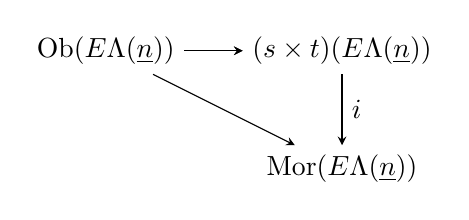
\begin{tikzpicture}[x=30mm,y=15mm]
		\node (a) at (0,0) {$\mathrm{Ob}(\ELn)$};
		\node (b) at (1,0) {$(s \times t)(\ELn)$};
		\node (d) at (1,-1) {$\mathrm{Mor}(\ELn)$};
      \draw [->] (a) to (b);
			\draw [->] (a) to node [above] {$$} (b);
			\draw [->] (b) to node [right] {$i$} (d);
			\draw [->] (a) to node [below,left] {$$} (d);
    \end{tikzpicture}
\end{center}		
\end{prop}
\begin{proof}
First, assume that the action operad $\ML$ is not crossed. Then there exists an obvious injective monoid homomorphism
% \[ \begin{array}{rlrll}
% 			i & \colon & (s \times t)(\ELn) & \rightarrow & \mathrm{Mor}(\ELn) \\
% 			& \colon & \mathbb{N}^{\ast n} & \rightarrow & \lop \times_{\mathbb{N}} \mathbb{N}^{\ast n} \\
% 			& \colon & w & \mapsto & ( \, e_{|w|}, w \, ),
% 		\end{array}
% \]
  \begin{align*}
    i \colon (s \times t)(\ELn) &\rightarrow \mathrm{Mor}(\ELn) \\
    w & \mapsto (e_{|w|}, w)
  \end{align*}
which is clearly seen when considering $i$ as a homomorphism $\mathbb{N}^{\ast n} \rightarrow \lop \times_{\mathbb{N}} \mathbb{N}^{\ast n} $ and where we have written $e_{|w|}$ for the identity in the group $\Lambda(|w|)$. The homomorphism property follows from the fact that the length $|w|$ defined in \cref{lengthdef} is itself a homomorphism, so $|w \oplus w'| = |w|+|w'|$. Thus $(s \times t)(\ELn) \subseteq \mathrm{Mor}(\ELn)$ for non-crossed $\ML$, and the splitting is obvious.

Now assume that $\ML$ is crossed. Fix a function $\rho$ as in \cref{rho_ww'}. Because $\mathbb{N}^{\ast n} \times_{\mathbb{N}^n} \mathbb{N}^{\ast n}$ is a free monoid  by \cref{freemon}, there is a unique monoid homomorphism
  \[
    \rho \colon \mathbb{N}^{\ast n} \times_{\mathbb{N}^n} \mathbb{N}^{\ast n} \longrightarrow \lop
  \]
which agrees with the original function $\rho$ on the generators in the source. By construction, we have
  \[
    \pi(\rho(w, w'))(w) = w'
  \]
for any $(w, w') \in\mathbb{N}^{\ast n} \times_{\mathbb{N}^n} \mathbb{N}^{\ast n}$, not just the generators. Using $\rho$ we define the homomorphism $i$ to be as follows.
  \begin{align*}
		i \colon (s \times t)(\ELn) &\rightarrow \mathrm{Mor}(\ELn) \\
		\mathbb{N}^{\ast n} \times_{\mathbb{N}^n} \mathbb{N}^{\ast n} &\rightarrow \lop \times_{\mathbb{N}} \mathbb{N}^{\ast n} \\
		(w, w') &\mapsto ( \, \rho(w, w'), w \, )
	\end{align*}
Moreover, for any two elements $(v, v')$, $(w, w')$ of $\mathbb{N}^{\ast n} \times_{\mathbb{N}^n} \mathbb{N}^{\ast n}$ we have
  \begin{align*}
		( \, \rho(v, v'), v \, )  =  ( \, \rho(w, w'), w \, ) & \implies \rho(v, v') \, = \, \rho(w, w'), \quad \quad v \, = \, w \\
		 & \implies v' \, = \, \pi(\rho(v, v'))(v) \, = \, \pi(\rho(w, w'))(w) \, = \, w'
  \end{align*}
%QQQ What is this actually saying? Needs rewriting more formally.
and thus $i$ is injective. This injection splits $\mathrm{Mor}(\ELn) \rightarrow (s \times t)(\ELn)$ by construction.

For the final statement, note that the inclusion of $\mathrm{Ob}(\ELn)$ into $(s \times t)(\ELn)$ sends an object $w$ to the pair $(w,w)$. The only indecomposable such are $(x_i, x_i)$ if we write the generating objects of $\ELn$ as $x_1, x_2, \ldots, x_n$. Using the construction above, we can always choose $\rho(x_i, x_i) = e_1$.
\end{proof}

For the proof of \cref{stGnsub}, $\rho$ can be any function satisfying the criteria in \cref{rho_ww'}, with the caveat that commuting with the inclusion of objects requires $\rho(x_i, x_i) = e_1$. The analogous proof for $L_n$, though, requires more properties of $\rho$ which we establish now. Recall the functor $\delta$ from \cref{qdef}. Note that by construction it restricts to a monoid homomorphism on sets of objects, and we denote this restriction by $\delta$ as well in the lemma below.

\begin{prop} \label{stZsub} $\MorLn \rightarrow (s \times t)(L_n)$ is a split epi of monoids, so $(s \times t)(L_n)$ is (isomorphic to) a submonoid of $\MorLn$. Furthermore, we can choose the injection $i \colon (s \times t)(L_n) \rightarrow \MorLn$ such that the following diagram commutes.
\begin{center}
    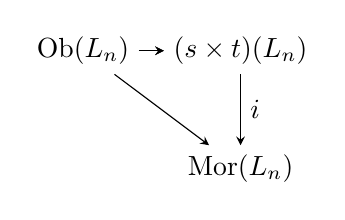
\begin{tikzpicture}[x=20mm,y=15mm]
		\node (a) at (0,0) {$\mathrm{Ob}(L_n)$};
		\node (b) at (1,0) {$(s \times t)(L_n)$};
		\node (d) at (1,-1) {$\MorLn$};
      \draw [->] (a) to (b);
			\draw [->] (a) to node [above] {$$} (b);
			\draw [->] (b) to node [right] {$i$} (d);
			\draw [->] (a) to node [below,left] {$$} (d);
    \end{tikzpicture}
\end{center}		
\end{prop}
\begin{proof}
Let $i \colon (s \times t)(\ELnn) \rightarrow \mathrm{Mor}(\ELnn)$ be a splitting as in \cref{stGnsub}. We will first show that the function $\rho$ can be chosen to make the square
\begin{center}
    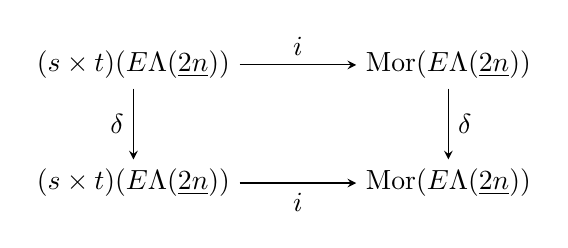
\begin{tikzpicture}[x=20mm,y=15mm]
		\node (a) at (0,0) {$(s \times t)(\ELnn)$};
		\node (b) at (2,0) {$\mathrm{Mor}(\ELnn)$};
		\node (c) at (0,-1) {$(s \times t)(\ELnn) $};
		\node (d) at (2,-1) {$\mathrm{Mor}(\ELnn)$};
			\draw [->] (a) to node [above] {$i$} (b);
			\draw [->] (b) to node [right] {$\delta$} (d);
			\draw [->] (a) to node [left] {$\delta$} (c);
			\draw [->] (c) to node [below] {$i$} (d);
    \end{tikzpicture}
\end{center}
commute. Recall that $i$ is defined by first factoring an element into indecomposables, and then applying $\rho$ to each of those. Thus on an indecomposable $(w,w')$, the commutativity of this square is the claim that $\delta(\rho(w,w')) = \rho(\delta w, \delta w')$ using that $\delta(w,w') = (\delta w, \delta w')$ is also indecomposable by the first part of \cref{rho_lemmas}. By the second part of \cref{rho_lemmas}, write $(w,w') = \delta^k(v,v')$ for a unique $(v, v')$ which is not in the image of $\delta$, so the equation $\delta(\rho(w,w')) = \rho(\delta w, \delta w')$ is equivalent to
  \[
    \delta\left(\rho\left(\delta^k(v,v')\right)\right) = \delta^{k+1}\rho(v,v').
  \]
Furthermore, $(v,v')$ cannot be written as $\delta(u,u')$ for any indecomposable $(u,u')$, so we may choose $\rho(v,v')$ arbitrarily and this will uniquely determine $i$ in such a way that the square commutes. 

The functor $q \colon \ELnn \rightarrow L_n$ is the cokernel of $\delta$, so the composite
  \[
    \mathrm{Mor}(\ELnn) \stackrel{\mathrm{Mor}\delta}{\longrightarrow} \mathrm{Mor}(\ELnn) \stackrel{\mathrm{Mor}q}{\longrightarrow} \MorLn
  \]
is the zero map. From the definition of $\delta$ in \cref{qdef} and the description of the monoids $(s \times t)(\ELn), (s \times t)(L_n)$ in \cref{stpullback}, the composite
  \[
    (s \times t)(\ELnn) \stackrel{(s \times t)(\delta)}{\longrightarrow}  (s \times t)(\ELnn) \stackrel{(s \times t)(q)}{\longrightarrow} (s \times t)(L_n)
  \]
exhibits $(s \times t)(L_n)$ as the cokernel of $(s \times t)(\delta)$ QQQ this is \cref{monoid_coeq} QQQ so induces a unique monoid homomorphism $i \colon  (s \times t)(L_n) \rightarrow \MorLn$ making the square below commute.
\begin{center}
    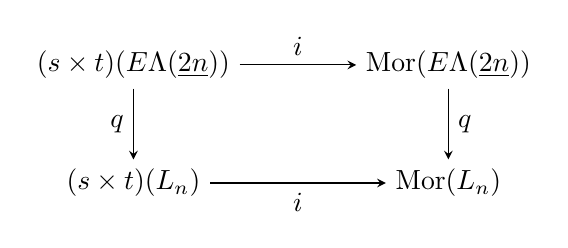
\begin{tikzpicture}[x=20mm,y=15mm]
		\node (a) at (0,0) {$(s \times t)(\ELnn)$};
		\node (b) at (2,0) {$\mathrm{Mor}(\ELnn)$};
		\node (c) at (0,-1) {$(s \times t)(L_n) $};
		\node (d) at (2,-1) {$\MorLn$};
			\draw [->] (a) to node [above] {$i$} (b);
			\draw [->] (b) to node [right] {$q$} (d);
			\draw [->] (a) to node [left] {$q$} (c);
			\draw [->] (c) to node [below] {$i$} (d);
    \end{tikzpicture}
\end{center}
This homomorphism $i$ splits $\MorLn \rightarrow (s \times t)(L_n)$ as desired.

The final claim about commuting with the inclusion of objects follows using the same argument as in  \cref{stGnsub}, so we must also require $\rho(x_i, x_i) = e_1$.

\end{proof} 

\section{Unit endomorphisms of \texorpdfstring{$L_n$}{L_n}}

We now consider the monoid of unit endomorphisms, $L_n(I,I)$. This is a particularly important submonoid of the morphisms $\MorLn$, since it is the only submonoid which is also a homset of the category $L_n$. Moreover, because the maps in $L_n(I,I)$ all share the same source and target, what we have is not just a monoid under tensor product but also under composition as well. This fact leads to a series of special properties for $L_n(I,I)$, the first of which is just another instance of the classic Eckmann-Hilton argument. 

\begin{prop} \label{endcom} $L_n(I,I)$ is a commutative monoid under both tensor product and composition, with $f \otimes f' = f \circ f'$. Since $L_n$ is a groupoid, this commutative monoid is actually an abelian group.
\end{prop}

In fact, we have the following corollary of \cref{tensinv_basic} in the case that $X = L_n$.

\begin{cor} \label{tensinv} Every morphism $f \colon  w \rightarrow v$ in $L_n$ has an inverse under tensor product, $f^* \colon  w^* \rightarrow v^*$. That is, the monoid $\MorLn$ is actually a group and $L_n(I,I)$ is a subgroup.
\end{cor}



\begin{prop} \label{endnorm} $L_n(I,I)$ is a normal subgroup of $\MorLn$. Moreover, if $\ML$ is a crossed action operad, then $L_n(I,I)$ is a subgroup of the center of $\MorLn$.
\end{prop}
\begin{proof}
From \cref{tensinv}, we know that $L_n(I,I)$ is a subgroup of $\MorLn$. For normality, we need to again consider both crossed and non-crossed cases separately. 

If $\ML$ is not crossed, then by \cref{crossconcomp} we know that the map assigning objects of $L_n$ to their connected component is just the identity $\id_{\mathbb{Z}^{\ast n}}$. In other words, every object belongs to its own unique component, so that every morphism of $L_n$ is actually an endomorphism. It follows that the group $L_n(I,I)$ is the kernel of the source homomorphism $s$ from \cref{st} and thus normal.

For crossed $\ML$, recall from \cref{spacial} that all $E\Lambda$-algebras are spacial, and so in particular $L_n$ is. This means that for any $h \in L_n(I,I)$ and $w \in \mathrm{Ob}(L_n)$ we will always have $h \otimes w = w \otimes h$. Thus for any $f \colon w \rightarrow v$ in $\MorLn$, we get
  \begin{align*}
  	h \otimes f & =(\id_I \circ h) \otimes (f \circ \id_w) \\
  	&= (I \otimes f) \circ (h \otimes w) \\
  	&= (f \otimes I) \circ (w \otimes h) \\
  	&= (f \circ \id_w) \otimes (\id_I \circ h) \\
  	&= f \otimes h
  \end{align*}
and so $L_n(I,I)$ is a subgroup of the center of $\MorLn$, thus normal. 
\end{proof}

\section{Splitting the monoid of morphisms}

In this section we will collect together many of the arguments of this chapter to give the first closed form expression for the automorphism group of the unit object, $I$, in $L_n$.
\begin{prop} \label{morprod} For any action operad $\ML$,
  \[
    \MorLn \quad \cong \quad (s \times t)(L_n) \ltimes L_n(I,I).
  \]
Moreover, if $\ML$ is a crossed action operad, then
  \[
    \MorLn \quad \cong \quad (s \times t)(L_n) \times L_n(I,I).
  \]
\end{prop}
\begin{proof}
We just saw in \cref{endnorm} that $L_n(I,I)$ is a normal subgroup of $\MorLn$, so we can consider the quotient group
\[ \begin{tikzcd}
L_n(I,I) \ar[r, hookrightarrow] & \MorLn \ar[r] & \bigquotient{\MorLn}{L_n(I,I)}
\end{tikzcd} \]
By the universal property of quotients, the map $\MorLn \rightarrow \MorLn / L_n(I,I)$ will uniquely factor any homomorphism whose composite with the inclusion $L_n(I,I) \hookrightarrow \MorLn$ is the zero map. But our source/target map $s \times t \colon \MorLn \rightarrow (s \times t)(L_n)$ is one such homomorphism, since for any $h \colon  I \rightarrow I$ clearly $(s \times t)(h) = (I, I)$, which is the identity element in $(s \times t)(L_n)$. Therefore there must exist a unique homomorphism $u$ making the triangle below commute:
\[ \begin{tikzcd}
\MorLn \ar[dd] \ar[ddrr, "s \times t"] & & \\
& & \\
\bigquotient{\MorLn}{L_n(I,I)} \ar[rr, "u"] & & (s \times t)(L_n)
\end{tikzcd} \]
This map $u$ will be surjective --- because $s \times t$ is --- but in fact it will also be injective. This is because if two morphisms $f, f'$ of $L_n$ have the same source and target, then the map $h = f^* \otimes f'$ is an element of $L_n(I,I)$ for which $f \otimes h = f'$, and so clearly $f$ and $f'$ are part of the same equivalence class in $\MorLn/L_n(I,I)$. 

Thus $u$ is bijective, so that
  \[
    \bigquotient{\MorLn}{L_n(I,I)} \cong (s \times t)(L_n)
  \]
and we have a group extension
\[ \begin{tikzcd}
0 \ar[r] & L_n(I,I) \ar[r, hookrightarrow] & \MorLn \ar[r, "s \times t"] & (s \times t)(L_n) \ar[r] & 0.
\end{tikzcd} \]
But recall from \cref{stZsub} that this extension is split, or equivalently $\MorLn$ is a semi-direct product $(s \times t)(L_n) \ltimes L_n(I,I)$. However, if $G$ is crossed then we also saw in \cref{endnorm} that $L_n(I,I)$ is a subgroup of the center of $\MorLn$, and so it will follow that $\MorLn$ is also a central extension of $(s \times t)(L_n)$. In that case $\MorLn$ is just the direct product $(s \times t)(L_n) \times L_n(I,I)$.
\end{proof}

\begin{cor}\label{lnII_mormodst}
If $\ML$ is crossed, then $L_n(I,I) \cong \MorLn / (s \times t)(L_n)$.
\end{cor}

\begin{conv}
In what follows (in particular, \cref{conseq_spl,full_des}), we fix an isomorphism $\MorLn \cong (s \times t)(L_n) \times L_n(I,I)$; we note that this isomorphism (and in particular the projection homomorphism $\MorLn \rightarrow L_n(I,I)$) depends on the choices made in the proof of \cref{stZsub}.

\end{conv}

\section{Splitting as a coherence theorem}\label{splitting_as_coh}

Coherence theorems often take the form of a statement that all diagrams with a certain property commute. For example, coherence for ordinary monoidal categories states that every diagram in the free monoidal category generated by a set of objects commutes and coherence for symmetric monoidal categories states that a pair of parallel morphisms (i.e., the two legs around some diagram of interest) are equal if and only if their underlying permutations are equal.

\begin{thm}\label{split_coh}
Let $\ML$ be an action operad, and $L_n$ the free $\ML$-monoidal category on $n$ invertible objects. Let $x, y$ be objects of $L_n$, and $f, g \colon  x \rightarrow y$ morphisms between them. Then the following are equivalent:
\begin{enumerate}
\item $f = g$,
\item $g^{-1} f = \id_x$, and
\item the automorphism of the unit object $x^{-1} \otimes \left(g^{-1} f\right)$ is the identity in $L_n(I,I)$.
\end{enumerate}
\end{thm}
\begin{proof}
1 implies 2 and 2 implies 3 are trivial. For 3 implies 1, we need only note that the invertibility of $x$ means that the function $x \otimes - \colon L_n(I,I) \rightarrow L_n(x,x)$ is a monoid isomorphism (with inverse $x^{-1} \otimes -$) so sends identities to identities.
\end{proof}

In practice, computing $x^{-1} \otimes \left(g^{-1} f\right)$ from $g^{-1} f$ is relatively simple, so we should view this theorem as affording the following strategy for resolving the potential equality of a pair of parallel morphisms $f, g \colon x \rightarrow y$.
\begin{enumerate}
\item Determine the group $L_n(I,I)$ in such a way as to make the equality of two elements computable in a practical fashion.
\item Compute $x^{-1} \otimes \left(g^{-1} f\right)$ as an element of this group.
\end{enumerate}
The following chapters are devoted to the first step of this strategy.

\chapter{Computing automorphisms of the unit}

Now we turn to the matter of computing the group $L_n(I,I)$. This group completely controls the morphisms which arise from the presence of $n$ different invertible objects as we saw in \cref{split_coh}. Our computations are necessarily of a different flavor from the theory we have so far established as the goal has changed from establishing the existence of this group to determining it explicitly with generators and relations.

\section{Nullary operations}
We will begin our computational investigations by first studying the nullary operations, the elements $g \in \Lambda(0)$.

\begin{lem} \label{noscalar} Let $m \in \mathbb{N}$ and let $\ML$ be an action operad. For any element $g \in \Lambda(m)$, the morphism
  \[
    g^{\otimes} \colon  I^m \rightarrow I^m
  \]
in $L_n$ is the identity.
Equivalently, for any element $h \in \Lambda(0)$, $h$ induces the identity morphism $I \rightarrow I$.
\end{lem}
\begin{proof}
First, let $g \in \Lambda(m)$. Then $g \colon  I^m \rightarrow I^m$ is equal to $q(g) \colon q(I^m) \rightarrow q(I^m)$ which is equal to $q\delta(g) \colon  q\delta(I^m) \rightarrow q\delta(I^m)$. Since $q$ is the coequalizer of $\delta$ and the zero map, $q\delta(g) = \id$ for all $g \in \Lambda(m)$. This clearly implies that every $h \in \Lambda(0)$ induces the identity map $I \rightarrow I$, but note that the morphism $g \colon I^m \rightarrow I^m$ is also the morphism induced by $\mu(g; e_0, \ldots, e_0) \in \Lambda(0)$, so these two claims are equivalent.
\end{proof}

This is a curious result. The morphisms $I \rightarrow I$ in $\ELn$ are exactly the elements of the group $\Lambda(0)$, but all of these become the identity in $L_n$. In other words, $L_n$ cannot detect any morphisms in $\Lambda(0)$, an idea we make precise in the next two results. 


\begin{prop} \label{G0quot} Let $\Lambda$ be a crossed action operad. Then there exists another crossed action operad $\Lambda'$ given by $\Lambda'(m) = \Lambda(m)/\Lambda(0)$ for all $m \in \mathbb{N}$.
\end{prop}
\begin{proof}
For any elements $g \in \Lambda(m)$ and $h \in \Lambda(0)$, their block sum $h \oplus g := \mu(e_2; h, g)$ is also an element of $\Lambda(m)$. Thus block sum defines a map $\Lambda(0) \times \Lambda(m) \rightarrow \Lambda(m)$, which is a group action by operad associativity and (QQQ previous lemma?) \cref{calclem}, and a group homomorphism by the action operad axioms and \cref{calclem}. This produces a homomorphism $\Lambda(0) \rightarrow \Lambda(m)$ for all $m$, which lies in the center of $\Lambda(m)$ by \cref{spacial}. Hence the image is normal for all $m$. Furthermore, the induced map $\Lambda(0) \rightarrow \Lambda(m) \rightarrow \Sigma_m$ is the zero map, so we have an induced homomorphism $\Lambda(m)/\Lambda(0) \rightarrow \Sigma_m$. All that remains to be shown is that the operadic multiplication for $\Lambda$ induces one for the groups $\Lambda(n)/\Lambda(0)$, and that this multiplication satisfies the axioms for an action operad.

Let $h, h_1, \ldots, h_m \in \Lambda(0)$ and $k_1, \ldots, k_m \in \mathbb{N}$. We have the following calculation using the action operad axioms for $\Lambda$ and the fact that $\EL(\underline{1})$ is spacial so the $e_k$ commute with all elements of $\Lambda(0)$.
\begin{align*}
		\mu^{\Lambda}\left( \, h \oplus e_m \, ; \, \underline{h_i \oplus e_{k_i}}\right) &= \mu^{\Lambda}\left( \, \mu^{\Lambda}(e_2; h, e_m) \, ; \, \underline{h_i \oplus e_{k_i}} \right) \\
		&= \mu^{\Lambda}\left( \, e_2 \, ; \, \mu^{\Lambda}(h;-), \mu^{\Lambda}(e_m; \underline{h_i \oplus e_{k_i}}) \right) \\
		&= \mu^{\Lambda}(h;-)\oplus \mu^{\Lambda}\left(e_m; \underline{h_i \oplus e_{k_i}}\right) \\
		&= h \oplus h_1 \oplus e_{k_1} \oplus \cdots \oplus h_m \oplus e_{k_m} \\
		&= e_{k_1} \oplus \cdots \oplus e_{k_m} \oplus h \oplus h_1 \cdots \oplus h_m \\
		&= e_{k_1+\cdots+k_m} \oplus h \oplus h_1 \cdots \oplus h_m
\end{align*}

The above shows that the following square commutes.
\begin{center}
    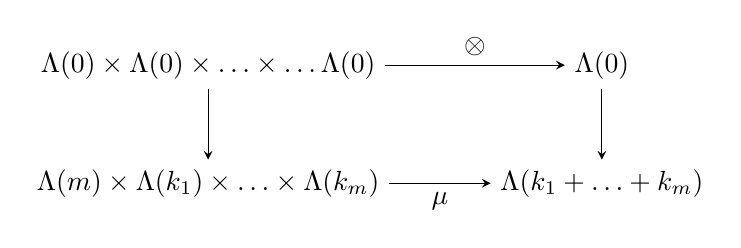
\begin{tikzpicture}[x=50mm,y=15mm]
		\node (a) at (0,0) {$ \Lambda(0) \times  \Lambda(0) \times \ldots \times \ldots  \Lambda(0)$};
		\node (b) at (1,0) {$\Lambda(0)$};
		\node (c) at (0,-1) {$ \Lambda(m) \times  \Lambda(k_1) \times \ldots \times  \Lambda(k_m) $};
		\node (d) at (1,-1) {$\Lambda(k_1 + \ldots + k_m)$};
			\draw [->] (a) to node [above] {$\otimes$} (b);
			\draw [->] (b) to node [right] {$$} (d);
			\draw [->] (a) to node [left] {$$} (c);
			\draw [->] (c) to node [below] {$\mu$} (d);
    \end{tikzpicture}
\end{center}	

We write the image of $g \in \Lambda(m)$ under the quotient $\Lambda(m) \rightarrow \Lambda'(m)$ as $[g]$. We will show that the multiplication
  \[
    \mu^{\Lambda'} \colon \Lambda'(m) \times \Lambda'(k_1) \times \cdots \times \Lambda'(k_m) \rightarrow \Lambda'(k_1 + \cdots + k_m)
  \]
given by 
  \[
    \mu^{\Lambda'}\left( [g]; [g_1], \ldots , [g_m] \right) = \left[\mu^{\Lambda}\left(g; g_1, \ldots, g_m \right)\right]
  \]
is well-defined. With $h, h_1, \ldots, h_m \in \Lambda(0)$ as above, we have
  \[
    \mu^{\Lambda}\left(g \cdot h \otimes e_m; g_1\cdot h_1 \otimes e_{k_1}, \ldots, g_m\cdot h_m \otimes e_{k_m} \right)
  \]
equals
  \[
    \mu^{\Lambda}(g; g_1, \ldots, g_m) \cdot \mu^{\Lambda}(h \otimes e_m; h_1 \otimes e_{k_1}, \ldots, h_m \otimes e_{k_m})
  \]
using the fact that $\pi(h \otimes e_m)$ is the identity permutation. By the commutative square above, $\mu^{\Lambda}(h \otimes e_m; h_1 \otimes e_{k_1}, \ldots, h_m \otimes e_{k_m})$ is in the image of $\Lambda(0) \rightarrow \Lambda(k_1 + \cdots + k_m)$, so $\mu^{\Lambda'}$ is well-defined. It is now straightforward to check the rest of the action operad axioms for $\Lambda'$ using those of $\Lambda$.
\end{proof}

We end this section by proving that the quotient action operad $\Lambda'$ removes the unnecessary nullary operations without changing the invertible objects.

\begin{thm} \label{noscalarcross} Let $\Lambda$ be a crossed action operad, and let $\Lambda'$ be the action operad with $\Lambda'(m) = \Lambda(m)/\Lambda(0)$ constructed in \cref{G0quot}. Then for any $n \in \mathrm{N}$,
  \[
    L\ML'_n \quad \cong \quad L\ML_n
  \]
both as $E\Lambda$-algebras and as $E\Lambda'$-algebras.  
\end{thm}
\begin{proof}
The quotient map $[-] \colon \ML \rightarrow \ML'$ induces a $\ML$-algebra structure on $L\ML'_n$, and hence produces a unique strict $\ML$-monoidal functor $L\ML_n \rightarrow L\ML'_n$ by the universal property of $L\ML_n$. $L\ML_n$ is also a $\ML'$-monoidal category by defining $[g]^{\otimes} \colon x_1 \otimes \cdots \otimes x_n \rightarrow x_{[g]^{-1}1} \otimes \cdots \otimes x_{[g]^{-1}n}$ to be $g^{\otimes}$. This is well-defined, as whenever we have $[g] = [h]$ it is because there is some $x \in \ML(0)$ for which $h = x \oplus g$. Then
  \[
    h^{\otimes} = (x \oplus g)^{\otimes} = x^{\otimes} \otimes g^{\otimes} = \id_I \otimes g^{\otimes} = g^{\otimes}
  \]
using \cref{otimesotimes}. Thus we also have an induced map $L\ML'_n \rightarrow L\ML_n$ using the universal property of $L\ML'_n$. By inspection, both of these functors preserve the $\ML$- and $\ML'$-actions, hence must be inverse to each other.
\end{proof}

\section{Reflexivity and a first calculation}

Recall that the functor $q \colon  \ELnn \rightarrow L_n$ expresses $L_n$ as a reflexive coequalizer of the morphisms $\delta, I$ of $\ML$-monoidal categories and hence also as a reflexive coequalizer of the morphisms $\tilde{\delta}, \tilde{I}$ of mere monoidal categories by \cref{q_other_coeq2}. We can therefore use the adjunction from \cref{Moradj} to calculate $\mathrm{M}(L_{n})^{\mathrm{gp, ab}}$. 

\begin{prop}\label{Zmor2} Let $\Delta$ be the subgroup of $\mathrm{M}(\ELnn)^{\mathrm{gp, ab}}$ generated by elements of the form
  \[
    \mathrm{M}(\tilde{\delta})^{\mathrm{gp, ab}}(f) \, - \, \mathrm{M}(\tilde{I})^{\mathrm{gp, ab}}(f)
  \]
for $f \in \mathrm{M}(\ELnnnn)^{\mathrm{gp, ab}}$.
Then the abelianization of the group completion of the collapsed morphisms of $L_n$ is computed as the quotient below.
  \[
    \mathrm{M}(L_{n})^{\mathrm{gp, ab}} \cong \bigquotient{{\mathrm{M}(\ELnn)}^{\mathrm{gp, ab}}}{\Delta}
  \]
\end{prop}
\begin{proof}
From \cref{Moradj}, we know that $\mathrm{M}(\, \_ \,)^{\mathrm{gp, ab}} \colon  \moncat \rightarrow \mb{Ab}$ is a left adjoint. This means that it preserves all colimits in $\moncat$, so
  \[
    \mathrm{coeq}\left( \, \mathrm{M}(\tilde{\delta})^{\mathrm{gp, ab}}, \, \mathrm{M}(\tilde{I})^{\mathrm{gp, ab}} \, \right) \cong \mathrm{M}\left( \, \mathrm{coeq}(\tilde{\delta}, \tilde{I}) \, \right)^{\mathrm{gp, ab}}.
  \]
The coequalizer of two abelian group homomorphisms is just the quotient of their common target by the image of their difference. Hence in this case we have
  \begin{align*}
    \mathrm{M}(L_{n})^{\mathrm{gp, ab}}  &\cong \bigquotient{{\mathrm{M}(\ELnn)}^{\mathrm{gp, ab}}}{Im\left( \, {\mathrm{M}(\tilde{\delta})}^{\mathrm{gp, ab}} - {\mathrm{M}(\tilde{I})}^{\mathrm{gp, ab}} \, \right)} \\
    & \cong \quad \bigquotient{{\mathrm{M}(\ELnn)}^{\mathrm{gp, ab}}}{\Delta}.
  \end{align*}
\end{proof} 

\begin{rem}\label{delta_neq_image}
Note that $Im(\mathrm{M}(\delta)^{\mathrm{gp, ab}})$ is a subgroup of $\Delta$ because $\delta$ factors through $\tilde{\delta}$.
\end{rem}



%QQQ Rewrite with better notation

Since our goal is to be able to make explicit computations of the group acting on a set of $n$ invertible objects in a $\ML$-monoidal category, we will need an explicit description of the elements of the subgroup $\Delta$.

QQQ Started rewriting with $g^{\otimes}$ notation but this needs more time than I have now.

\begin{lem} $\Delta$ is the subgroup of $\mathrm{M}(\ELnn)^{\mathrm{gp, ab}}$ whose elements are tensor products of the equivalence classes
  \[
		\left[ \, \alpha^{\ELnn}\left( \, \mu( \, g \, ; \, e_{\left|\tilde{\delta}(x_1)\right|}, \ldots, e_{\left|\tilde{\delta}(x_m)\right|} \, ) \, ; \, \id_{x'_1}, \ldots,  \id_{x'_{m'}} \, \right) \, \right] \\
  \]
and
  \[
		\left[ \, \alpha^{\ELnn}\left( \, \mu( \, g \, ; \, e_{\left|\tilde{I}(x_1)\right|}, \ldots, e_{\left|\tilde{I}(x_m)\right|} \, ) \, ; \, \id_{x''_1}, \ldots,  \id_{x''_{m''}} \, \right) \, \right]^*
  \]
where $g \in G(m)$, the $x_i$ are generators of $\mathbb{N}^{\ast 4n}$, the $x'_i, x''_i$ are generators of $\mathbb{N}^{\ast 2n}$, and
  \begin{align*}
  	\tilde{\delta}( x_1 \otimes \ldots \otimes x_m) & =  x'_1 \otimes \ldots \otimes x'_{m'}, \\
  	\tilde{I}( x_1 \otimes \ldots \otimes x_m) & =  x''_1 \otimes \ldots \otimes x''_{m''}.
  \end{align*}
\end{lem}
\begin{proof}  
Let $f$ be an element of $\mathrm{M}(\mathbb{G}_{4n})^{\mathrm{gp, ab}}$. By definition this means that $f$ is an equivalence class of morphisms from $\mathbb{G}_{4n}$, and so by \cref{hom-set-lemma} there must exist $g \in G(m)$ and $x_1, \ldots, x_m \in \{ z_1, \ldots, z_{4n} \}$ for which
  \[
    f \quad = \quad \left[g^{\otimes}\right].
  \]
Thus
  \begin{align*}
		\mathrm{M}(\tilde{\delta})^{\mathrm{gp, ab}}(f) &= \mathrm{M}(\tilde{\delta})^{\mathrm{gp, ab}} \left(\,\left[g^{\otimes} \right] \,\right) \\
		&= \left[ \, \tilde{\delta}\left(g^{\otimes}\right) \, \right]  
  \end{align*}
which is $g^{\otimes}$ acting on the tensor product $\tilde{\delta}(x_1) \otimes \tilde{\delta}(x_2) \otimes \ldots \otimes \tilde{\delta}(x_n)$.
By \cref{hom-set-lemma}, we can express this isomorphism as $h^{\otimes}$ for some $h \in \Lambda(p)$ we know it must be possible to express the action morphism $\alpha^{\ELnn}(g; \id_{\tilde{\delta}(x_1)}, \ldots, \id_{\tilde{\delta}(x_m)})$ as an action morphism on the identities of generators. Since the source of this map is
  \[
    \tilde{\delta}(x_1) \otimes \ldots \otimes \tilde{\delta}(x_m) = \tilde{\delta}(x_1 \otimes \ldots \otimes x_m) =: x'_1 \otimes \ldots \otimes x'_{m'}
  \]
clearly the $x'_i$ are the generators we want. So by expanding the $\tilde{\delta}(x_i)$ as tensor products of these we find that
  \[
    % \left[ \, \alpha^{\ELnn}(g; \id_{\tilde{\delta}(x_1)}, \ldots, \id_{\tilde{\delta}(x_m)})  \, \right] \quad = \quad \left[ \, \alpha^{\ELnn}\left( \, \mu( \, g \, ; \, e_{|\tilde{\delta}(x_1)|}, \ldots, e_{|\tilde{\delta}(x_m)|} \, ) \, ; \, \id_{x'_1}, \ldots, \id_{x'_{m'}} \, \right) \, \right]
    \left[ \, \alpha^{\ELnn}\left(g; \underline{\id_{\tilde{\delta}(x_i)}}\right) \, \right] = \left[ \, \alpha^{\ELnn}\left( \, \mu\left( \, g \, ; \, \underline{e_{\left|\tilde{\delta}(x_i)\right|}}\, \right) \, ; \, \underline{\id_{x'_j}}\, \right) \, \right]
  \]
where
  \begin{align*}
    \underline{\id_{\tilde{\delta}(x_i)}} &= \id_{\tilde{\delta}(x_1)}, \ldots, \id_{\tilde{\delta}(x_m)}, \\
    \underline{e_{\left|\tilde{\delta}(x_i)\right|}} &= e_{|\tilde{\delta}(x_1)|}, \ldots, e_{\left|\tilde{\delta}(x_m)\right|}, \\
    \underline{\id_{x'_j}} &= \id_{x'_1}, \ldots, \id_{x'_{m'}}.
  \end{align*}
For analogous reasons we also get
\begin{align*}
			\mathrm{M}(\tilde{I})^{\mathrm{gp, ab}}(f) & = \left[ \, \alpha^{\ELnn}\left(g; \id_{\tilde{I}(x_1)}, \ldots, \id_{\tilde{I}(x_m)}\right) \, \right]  \\
			&=  \left[ \, \alpha^{\ELnn}\left( \, \mu\left( \, g \, ; \, e_{|\tilde{I}(x_1)|}, \ldots, e_{|\tilde{I}(x_m)|} \, \right) \, ; \, \id_{x''_1}, \ldots,  \id_{x''_{m''}} \, \right) \, \right]
\end{align*}
and using these equations the lemma follows immediately from the definition of $\Delta$.
\end{proof}




\section{Consequences of the splitting}\label{conseq_spl}

In this section we will combine our splitting result (\cref{morprod}) with the quotients in the previous section.

\begin{cor}\label{Zmor1} Let $\ML$ be a crossed action operad. Then the endomorphisms of the unit object of $L_n$ are
  \[
    L_n(I, I) \quad \cong \quad \bigquotient{{\MorLn}^{\mathrm{ab}}}{{(s \times t)(L_n)}^{\mathrm{ab}}}
  \]
and therefore
  \[
    \MorLn \quad \cong \quad (s \times t)(L_n) \, \times \, \bigquotient{{\MorLn}^{\mathrm{ab}}}{{(s \times t)(L_n)}^{\mathrm{ab}}}.
  \]
\end{cor}
\begin{proof}
Both statements follow from the simple fact that abelianization preserves products and quotients.
\end{proof}

\begin{lem} \label{colquot} Let $X$ be any monoidal category whose objects and morphisms are all invertible under tensor product (see \cref{def_tensinv} and \cref{tensinv}). Then the monoid of collapsed morphisms (see \cref{def:M}) $\mathrm{M}(X)$ is already a group, and its abelianization is isomorphic to $\mathrm{Mor}(X)^{\mathrm{ab}}/ \mathrm{Ob}(X)^{\mathrm{ab}}$.
\end{lem}
\begin{proof}
Note that both $\mathrm{Mor}(X)$ and $\mathrm{M}(X)$ are groups by assumption. Let  $f \colon  x \rightarrow y$, $f' \colon  y \rightarrow z$ be a composable pair of morphisms in $X$. Recall  that in any monoidal category with invertible objects,
  \[
    f' \circ f = f' \otimes \id_{y^{-1}} \otimes f
  \]
by \cref{tenscomp}.  But $f' \otimes f = f' \circ f$ in $\mathrm{M}(X)$ by definition, so $\id_y$ is the identity element $e$ in $\mathrm{M}(X)$, and hence also $\mathrm{M}(X)^{\mathrm{ab}}$, for any object $y$.

Now let $A$ be an abelian group and $\phi \colon  \mathrm{Mor}(X)^{\mathrm{ab}} \rightarrow A$ be any homomorphism of groups which satisfies the condition $\phi(\mathrm{ab}(\id_x)) = e$ for all objects $x$. Then
\begin{align*}
			\phi\left( \, \mathrm{ab}(f' \circ f) \, \right)  &= \phi\left( \, \mathrm{ab}(f' \otimes \id_{y^{-1}} \otimes f) \, \right) \\
			&= \phi\left( \, \mathrm{ab}(f') \, \right) \otimes \phi\left( \, \mathrm{ab}(\id_{y^{-1}}) \, \right) \otimes \phi\left( \, \mathrm{ab}(f) \, \right) \\
			&= \phi\left( \, \mathrm{ab}(f') \, \right) \otimes \phi\left( \, \mathrm{ab}(f) \, \right) \\
			&= \phi\left( \, \mathrm{ab}(f' \otimes f) \, \right),
		\end{align*}
but using \cref{Morder} it is easy to see that this is the defining relation for the group $\mathrm{M}(X)^{\mathrm{ab}}$, so $\mathrm{M}(X)^{\mathrm{ab}}$ and $\mathrm{Mor}(X)^{\mathrm{ab}}/\mathrm{Ob}(X)^{\mathrm{ab}}$ have the same universal property and are therefore uniquely isomorphic under $\mathrm{Mor}(X)^{\mathrm{ab}}$.
\end{proof}

Here is the main theorem of this section, a first description of $L_n(I,I)$.

\begin{thm}
For any crossed action operad $\ML$, 
  \[
    L_n(I,I) \cong \frac{\left(\quotient{{\mathrm{M}(\ELnn)}^{\mathrm{gp},\mathrm{ab}}}{\Delta}\right)}{\left(\quotient{{(\mathbb{Z}^{\ast n} \times_{\mathbb{Z}^n} \mathbb{Z}^{\ast n})}^{\mathrm{ab}}}{\mathbb{Z}^n}\right)}, 
  \]
and the monoid of morphisms of $L_n$ is therefore
  \[ 
    \MorLn \cong \mathbb{Z}^{\ast n} \times_{\mathbb{Z}^n} \mathbb{Z}^{\ast n}  \, \times \, \frac{\left(\quotient{{\mathrm{M}(\ELnn)}^{\mathrm{gp},\mathrm{ab}}}{\Delta}\right)}{\left(\quotient{{(\mathbb{Z}^{\ast n} \times_{\mathbb{Z}^n} \mathbb{Z}^{\ast n})}^{\mathrm{ab}}}{\mathbb{Z}^n}\right)}.
  \]
\end{thm}
\begin{proof}
We have the isomorphism
  \[
    L_n(I,I) \cong \bigquotient{{\MorLn}^{\mathrm{ab}}}{{(s \times t)(L_n)}^{\mathrm{ab}}}
  \]
from \cref{Zmor1}. Note that this quotient  depends on the embedding of $(s \times t)(L_n)$ as a subgroup of the morphisms $L_n$ in \cref{stZsub}. The proof there ensured that the embedding we construct commutes with the inclusion of the monoid of objects, so
  \[
    \bigquotient{{\MorLn}^{\mathrm{ab}}}{{(s \times t)(L_n)}^{\mathrm{ab}}} \cong \frac{\left(\quotient{{\MorLn}^{\mathrm{ab}}}{\mathrm{Ob}(L_n)^{\mathrm{ab}}}\right)}{\left(\quotient{{(s \times t)(L_n)}^{\mathrm{ab}}}{\mathrm{Ob}(L_n)^{\mathrm{ab}}}\right)}.
  \]


Using \cref{colquot} to change the numerator and \cref{Zobj,stpullback} to simplify the denominator, this quotient becomes
  \[
    \bigquotient{{\MorLn}^{\mathrm{ab}}}{{(s \times t)(L_n)}^{\mathrm{ab}}} \cong \frac{\left(\quotient{{\mathrm{M}(\ELnn)}^{\mathrm{gp},\mathrm{ab}}}{\Delta}\right)}{\left(\quotient{{(\mathbb{Z}^{\ast n} \times_{\mathbb{Z}^n} \mathbb{Z}^{\ast n})}^{\mathrm{ab}}}{\mathbb{Z}^n}\right)}
  \]
as desired.
\end{proof}

It should be clear that there is further work to do in order to give a usable construction of the category $L_n$ and the group $L_n(I,I)$. We will spend the next two sections performing the necessary algebra to interpret the complicated parts of the formula above, namely $(\mathbb{Z}^{\ast n} \times_{\mathbb{Z}^n} \mathbb{Z}^{\ast n})^{\mathrm{ab}}$ and ${\mathrm{M}(\ELnn)}^{\mathrm{gp},\mathrm{ab}}$.

\section{Calculation: abelianizing sources and targets}
 
 Our first calculation will give a presentation for $(\mathbb{Z}^{\ast n} \times_{\mathbb{Z}^n} \mathbb{Z}^{\ast n})^{\mathrm{ab}}$. We were able to prove that $\mathbb{N}^{\ast n} \times_{\mathbb{Z}^N} \mathbb{N}^{\ast n}$ is a free monoid, but one cannot then conclude that $\mathbb{Z}^{\ast n} \times_{\mathbb{Z}^n} \mathbb{Z}^{\ast n}$ is a free group since group completion is a left adjoint and does not commute with pullbacks. Abelianization is also a left adjoint, and we cannot commute it past the pullback for the same reason. Thus we give a presentation directly. For the reader uninterested in the algebra involved, we record the main results of this section now:
 %QQQ Change the wording of this.
 \begin{itemize}
 \item we prove
  \[
    (\mathbb{Z}^{\ast n} \times_{\mathbb{Z}^n} \mathbb{Z}^{\ast n})^{\mathrm{ab}} \cong \mathbb{Z}^n \times {\mathbb{Z}}^{\binom{n}{2}}
  \]
 in \cref{abst} and
 \item we prove
  \[ 
    \bigquotient{{(\mathbb{Z}^{\ast n} \times_{\mathbb{Z}^n} \mathbb{Z}^{\ast n})}^{\mathrm{ab}}}{\mathbb{Z}^n} \cong \mathbb{Z}^{\binom{n}{2}} 
  \]
in \cref{nchoose2}.
 \end{itemize}

\begin{prop} \label{pushpres} The pullback group $\mathbb{Z}^{\ast n} \times_{\mathbb{Z}^n} \mathbb{Z}^{\ast n}$ is generated by two families of elements,
  \[
    \langle x \rangle \quad := \quad (x, x)
  \]
and
  \[
    \langle xy \rangle \quad := \quad (xy, yx)
  \]
where $x,y \in \{z_1, \ldots, z_n, z_1^*, \ldots, z_n^*\}$ are generators of the free group $\mathbb{Z}^{\ast n}$ or their inverses. These are subject to the following relations.
  \[
    \begin{array}{c}
			\langle x \rangle^{-1}  =  \langle x^* \rangle,  \quad  \langle xy \rangle^{-1}  =  \langle y^*x^* \rangle \\
			\\
			\langle xx^* \rangle  =  e  =  \langle x^*x \rangle,  \quad  \langle xx \rangle  =  \langle x \rangle^2 \\
			\\
			\langle xy \rangle \langle x^* \rangle \langle xy^* \rangle  =  \langle x \rangle \\
			\\
			\langle xy \rangle \langle x^* \rangle \langle y^* \rangle \langle yx \rangle  =  \langle x \rangle \langle y \rangle   =  \langle yx \rangle \langle x^* \rangle \langle y^* \rangle \langle xy \rangle \\
			\\
			\langle xy \rangle \langle x^* \rangle \langle xz \rangle \langle x^* \rangle \langle z^* \rangle \langle y^* \rangle \langle yz \rangle \langle y^* \rangle \langle yx \rangle \langle y \rangle \langle x^* \rangle \langle z^* \rangle^{-1} \langle zx \rangle \langle z^* \rangle \langle zy \rangle  =  \langle x \rangle\langle y \rangle\langle z \rangle 
  	\end{array}
  \]
\end{prop}
\begin{proof}
We'll begin by constructing a certain monoidal category, which we will call $Z$. 
\begin{itemize}
\item The objects of $Z$ are the elements of the group $\mathbb{Z}^{\ast n}$, with the usual multiplication as the tensor product.
\item There is a unique morphisms between any two objects $x$ and $y$ for which $\mathrm{ab}(x) = \mathrm{ab}(y)$, where $\mathrm{ab} \colon  \mathbb{Z}^{\ast n} \rightarrow \mathbb{Z}^n$ is the quotient map of abelianization. In other words, the morphisms of $Z$ are the elements of $\mathbb{Z}^{\ast n} \times_{\mathbb{Z}^n} \mathbb{Z}^{\ast n}$, with multiplication as the tensor product and composition given by
  \[
    (x,y) \circ (y,z)  =  (x, z)
  \]
\item The identity map on an object $x$ is then the unique map $(x,x) \colon x \rightarrow x$.
\end{itemize}
$Z$ is almost the subcategory of $L_n$ whose morphisms are the subgroup isomorphic to $(s \times t)(L_n)$ that we chose in \cref{stZsub}. However, we never required those representatives to be closed under composition, so $Z$ is a strictly formal version of the subcategory on $(s \times t)(L_n)$, one that doesn't involve any specific choice of the map $\rho$. It is a well-defined monoidal category; the only thing that might not be immediately clear is the law of interchange, which is just given by
  \begin{align*}
  	\left((x,y) \circ (y,z) \right) \otimes \left(  (x',y') \circ (y',z')  \right) &= (x,z) \otimes (x',z') \\
  	&= (xx',zz') \\
  	&= (xx',yy') \circ (yy',zz') \\
  	&= \left(  (x,y) \otimes (x',y')  \right) \circ \left(  (y,z) \otimes (y',z')  \right).
  \end{align*}
But now recall from \cref{tenscomp} that in any monoidal category the composition of morphisms along an intertible object can be rewritten in terms of only the tensor product. In the case of $Z$, where all of the objects have inverses, we will have
  \[
    (x,y) \circ (y, z)  =  (x, y) \otimes (y^*, y^*) \otimes (y, z)
  \]
Using this composition operation will make it easier to understand the structure of the group $\mathbb{Z}^{\ast n} \times_{\mathbb{Z}^n} \mathbb{Z}^{\ast n}$.

Next, let $\mathbb{S}_{2n}$ be the free $\mathrm{E}S$-algebra on $2n$ objects, where $S$ is the symmetric action operad. Then there is an obvious monoidal functor $\psi \colon \mathbb{S}_{2n} \rightarrow Z$, given as follows.
  \begin{align*}
		 \psi(z_i) &= z_i \\
		 \psi(z_{n+i}) &= z_i^* \\
		 \psi(\alpha(\sigma; \id_{x_1}, \ldots, \id_{x_m})) &= (x_1 \otimes \ldots \otimes x_m, x_{\sigma(1)} \otimes \ldots \otimes x_{\sigma(m)})
	\end{align*}
A necessary condition for $(y, y')$ to be an element of $\mathbb{Z}^{\ast n} \times_{\mathbb{Z}^n} \mathbb{Z}^{\ast n}$ is that there exists some sequence of generators and their inverses $x_1, \ldots, x_m \in \{z_1, \ldots, z_n, z_1^*, \ldots, z_n^*\}$ and some permutation $\sigma \in \Sigma_m$ for which
  \begin{align*}
    y &= x_1 \otimes \ldots \otimes x_m,\\
    y' &= x_{\sigma(1)} \otimes \ldots \otimes x_{\sigma(m)}.
  \end{align*}
Hence the functor $\psi$ is clearly surjective. It follows from this that if we can find a collection of morphisms which generate $\mathrm{Mor}(\mathbb{S}_{2n})$ under composition and tensor product, their images under $\psi$ will also generate $\mathrm{Mor}(Z) = \mathbb{Z}^{\ast n} \times_{\mathbb{Z}^n} \mathbb{Z}^{\ast n}$ under composition and tensor product, and hence under just tensor product. To begin, we know that any permutation $\sigma \in \Sigma_m$ can be written as a product $\sigma_{i_k} \cdot \ldots \cdot \sigma_{i_1}$ of elementary transpositions, giving
  \begin{align*}
  	\alpha( \, \sigma \, ; \, \id_{x_1}, \ldots, \id_{x_m} \, ) = & \alpha( \, \sigma_{i_k} \cdot \ldots \cdot \sigma_{i_1} \, ; \,  \id_{x_1}, \ldots, \id_{x_m} \, ) \\
  	= &\alpha( \, \sigma_{i_1} \, ; \,  \id_{x_1}, \ldots, \id_{x_m} \, )  \\
  	&\circ \, \alpha( \, \sigma_{i_2} \, ; \,  \id_{x_{\sigma_{i_1}(1)}}, \ldots, \id_{x_{\sigma_{i_1}(m)}} \, ) \, \circ \ldots \\
  	&\circ \, \alpha( \, \sigma_{i_k} \, ; \,  \id_{x_{\sigma_{i_{k-1}} \cdot \ldots \cdot \sigma_{i_1}(1)}}, \ldots, \id_{x_{\sigma_{i_{k-1}} \cdot \ldots \cdot \sigma_{i_1}(m)}} \, ).
  \end{align*}
Then if $\sigma_i = (i \, \, i+1) \in \Sigma_m$ is some elementary transposition we will have
  \begin{align*}
  	\alpha((i \, \, \, i+1) ; \id_{x_1}, \ldots, \id_{x_m} ) &= \alpha(e_{i-1} \otimes (1 \, \, \,2) \otimes e_{m-i-1};  \id_{x_1}, \ldots, \id_{x_m} ) \\
  	& =\id_{x_1 \otimes \ldots \otimes x_{i-1}} \otimes \alpha((1 2);\id_{x_i}, \id_{x_{i+1}}) \otimes \id_{x_{i+2} \otimes \ldots \otimes x_m}
  \end{align*}
Therefore all of the morphisms of $\mathbb{S}_{2n}$ are generated by just the identities and the action maps $\alpha((1 \, \, \, 2);\id_{x_1}, \id_{x_2})$ for all pairs $x_1, x_2 \in \{z_1, \ldots, z_{2n} \}$. Passing through $\psi$, this means that elements of $\mathbb{Z}^{\ast n} \times_{\mathbb{Z}^n} \mathbb{Z}^{\ast n}$ can always be expressed as a tensor product of elements of the form $(x, x)$ or $(x y, y x)$, where $x, y \in \{z_1, \ldots, z_n, z_1^*, \ldots, z_n^* \}$. These are exactly the $\langle x \rangle$ and $\langle xy \rangle$ given in the statement of the proposition.

Now we need to consider what relations these generators will obey. Firstly, their definitions overlap in the following case:
  \[
    \langle xx \rangle = (xx,xx) = (x,x) \otimes (x,x) = \langle x \rangle\langle x \rangle.
  \]
Next we have to account for the law of interchange we discussed earlier. Using \cref{tenscomp}, we see that this condition will induce the following relation:
  \begin{align*}
  	\langle xy \rangle \langle x^* \rangle \langle y^* \rangle \langle yx \rangle & = (xy, yx) \otimes (x^*, x^*) \otimes (y^*, y^*) \otimes (yx, xy) \\
  	& = (xy, yx) \otimes (yx, yx)^* \otimes (yx, xy) \\
  	& = (xy,yx) \circ (yx, xy) \\
  	& = (yx, xy) \otimes (yx, yx)^* \otimes (yx, xy) \\
  	& = (yx, xy) \otimes (x^*, x^*) \otimes (y^*, y^*) \otimes (xy, yx) \\
  	& = \langle yx \rangle \langle x^* \rangle \langle y^* \rangle \langle xy \rangle.
  \end{align*}
Also, by functoriality these generators will inherit any relations are obeyed to the corresponding morphisms of $\mathbb{S}_{2n}$, which in turn are just relations among different elementary transpositions. Each symmetric group $\Sigma_m$ is subject to three families of these, namely:
  \begin{align*}
  	(\sigma_i)^2 & = e \\
  	\sigma_i \sigma_j & = \sigma_j \sigma_i, \quad j \neq i \pm 1 \\
  	(\sigma_i \sigma_{i+1})^3 & = e
  \end{align*}
The first one, the symmetry condition, corresponds to the relation
%QQQ Unclear again. Needs writing with words, not \implies.
\[ \begin{array}{rrll}
			& (xy, yx) \circ (yx, xy) & = & (xy, xy) \\
			\implies & (xy, yx) \otimes (yx, yx)^* \otimes (yx, xy) & = & (x, x) \otimes (y,y) \\
			\implies & (xy, yx) \otimes (x^*, x^*) \otimes (y^*, y^*)  \otimes (yx, xy) & = & (x, x) \otimes (y,y) \\
			\implies & \langle xy \rangle\langle x^* \rangle\langle y^* \rangle\langle yx \rangle & = & \langle x \rangle\langle y \rangle \\
		\end{array}
\]
The second relation is just an example of interchange, which we have already looked at. The third yields the fact that
  \[
    \resizebox{\textwidth}{!}{$(xy, yx)(x^*,x^*)(xz,zx)(x^*,x^*)(z^*,z^*)(y^*,y^*)(yz,zy)(y^*,y^*)(yx,xy)(y^*,y^*)(x^*,x^*)(z^*,z^*)(zx, xz)(z^*,z^*)(zy,yz)$}
  \]
is equal to $(x,x)(y,y)(z,z)$. Or simply
  \[
    \langle xy \rangle \langle x^* \rangle \langle xz \rangle \langle x^* \rangle \langle z^* \rangle \langle y^* \rangle \langle yz \rangle \langle y^* \rangle \langle yx \rangle \langle y^* \rangle \langle x^* \rangle \langle z^* \rangle \langle zx \rangle \langle z^* \rangle \langle zy \rangle \quad = \quad \langle x \rangle\langle y \rangle\langle z \rangle.
  \]
Finally, we need to check how the invertibility of the objects of $Z$ interacts with these generators. Most obviously, we have
  \begin{align*}
  	\langle x \rangle^{-1} & = (x, x)^* = (x^*, x^*) = \langle x^* \rangle, \\
  	\langle xy \rangle^{-1} & = (xy, yx)^* = (y^*x^*, x^*y^*) = \langle y^*x^* \rangle \\
  \end{align*}
and
  \begin{align*}
  	\langle xx^* \rangle & = (xx^*, x^*x)= (I, I) = e, \\
  	\langle x^*x \rangle & = (x^*x, xx^*)= (I,I) = e. \\
  \end{align*}
But we can also insert an element and its inverse into different points of the source and target:
  \begin{align*}
  	\langle x \rangle & = (x,x) \\
  	& = (xyy^*, yy^*x) \\
  	& = (xyy^*, yxy^*) \circ (yxy^*, yy^*x) \\
  	& = (xyy^*, yxy^*) \otimes (yxy^*, yxy^*)^* \otimes (yxy^*, yy^*x) \\
  	& = (xy, yx) \otimes (y^*,y^*) \otimes (y, y) \otimes (x,x)^*(y^*, y^*) \otimes (y, y) \otimes (xy^*, y^*x) \\
  	& = \langle xy \rangle \langle x^* \rangle \langle xy^* \rangle.
  \end{align*}
The relations $(xy, yx) = (zz^*xy, yzz^*x)$ and so forth are all composed of successive instance of the above, so these are all of the relations on our generators $\langle x \rangle$ and $\langle xy \rangle$.
\end{proof}

\begin{prop} \label{abst}
%QQQ Write some words.
  \[
    (\mathbb{Z}^{\ast n} \times_{\mathbb{Z}^n} \mathbb{Z}^{\ast n})^{\mathrm{ab}} \cong \mathbb{Z}^n \times {\mathbb{Z}}^{\binom{n}{2}}
  \]
\end{prop}
\begin{proof}
It follows immediately from \cref{pushpres} that the group $(\mathbb{Z}^{\ast n} \times_{\mathbb{Z}^n} \mathbb{Z}^{\ast n})^{\mathrm{ab}}$ has a presentation on generators
\[ \langle x \rangle, \quad \langle xy \rangle, \quad x,y \in \{z_1, \ldots, z_n, z_1^*, \ldots, z_n^*\} \]
subject to the relations
%QQQ Check these before messing about with the code.
\[ \begin{array}{c}
			\langle x \rangle^{-1} \quad = \quad \langle x^* \rangle, \quad \quad \quad \langle xy \rangle^{-1} \quad = \quad \langle y^*x^* \rangle \\
			\\
			\langle xx^* \rangle \quad = \quad e \quad = \quad \langle x^*x \rangle, \quad \quad \quad \langle xx \rangle \quad = \quad \langle x \rangle^2 \\
			\\
			\langle xy \rangle \langle x^* \rangle \langle xy^* \rangle \quad = \quad \langle x \rangle  \\
			\\
			\langle xy \rangle \langle x^* \rangle \langle y^* \rangle \langle yx \rangle \quad = \quad \langle x \rangle \langle y \rangle  \quad = \quad \langle yx \rangle \langle x^* \rangle \langle y^* \rangle \langle xy \rangle \\
			\\
			\langle xy \rangle \langle x^* \rangle \langle xz \rangle \langle x^* \rangle \langle z^* \rangle \langle y^* \rangle \langle yz \rangle \langle y^* \rangle \langle yx \rangle \langle y^* \rangle \langle x^* \rangle \langle z^* \rangle \langle zx \rangle \langle z^* \rangle \langle zy \rangle \quad = \quad \langle x \rangle\langle y \rangle\langle z \rangle 
		\end{array}
\]
but then also the commutativity conditions
\[ \langle x \rangle \langle y \rangle \, = \, \langle y \rangle \langle x \rangle, \quad \quad \langle x \rangle \langle yz \rangle \, = \, \langle z \rangle \langle xy \rangle, \quad \quad	\langle wx \rangle \langle yz \rangle \, = \, \langle yz \rangle \langle wx \rangle \] 
Rearranging all of the former equations with the latter in mind, we get
\[ \begin{array}{c}
			\langle x \rangle^{-1} \quad = \quad \langle x^* \rangle, \quad \quad \quad \langle xy \rangle^{-1} \quad = \quad \langle y^*x^* \rangle \\
			\\
			\langle xx^* \rangle \quad = \quad e \quad = \quad \langle x^*x \rangle, \quad \quad \quad \langle xx \rangle \quad = \quad \langle x \rangle^2  \quad = \quad \langle xy \rangle \langle xy^* \rangle \\
			\\
			\langle xy \rangle \langle yx \rangle \quad = \quad \langle x \rangle^2 \langle y \rangle^2 \\
			\\
			\langle xy \rangle \langle yx \rangle \langle xz \rangle \langle zx \rangle \langle yz \rangle \langle zy \rangle \quad = \quad \langle x \rangle^4 \langle y \rangle^4 \langle z \rangle^4 
		\end{array}
\]
The last of these relations is just a consequence of the one above that,
\[ \begin{array}{rll}
			\langle xy \rangle \langle yx \rangle \langle xz \rangle \langle zx \rangle \langle yz \rangle \langle zy \rangle & = & \left( \, \langle x \rangle^2 \langle y \rangle^2 \, \right)\left( \, \langle x \rangle^2 \langle z \rangle^2 \, \right)\left( \, \langle y \rangle^2 \langle y \rangle^2 \, \right) \\
			& = & \langle x \rangle^4 \langle y \rangle^4 \langle z \rangle^4 
		\end{array}
\]
and in turn, the second-to-last follows from the relation above it,
\[ \begin{array}{rll}
			\langle x \rangle^2 \langle y \rangle^2  & = & \left( \, \langle xy \rangle \langle xy^* \rangle \, \right)\left( \, \langle yx \rangle \langle yx^* \rangle \, \right) \\
			& = & \langle xy \rangle \langle yx \rangle \langle xy^* \rangle  \langle xy^* \rangle^{-1} \\
			& = & \langle xy \rangle \langle yx \rangle
		\end{array}
\]
Without these, we are just left with equations in two or fewer variables. Then for any two $z_i, z_j \in \mathbb{Z}^{\ast n}$, $i<j$, the first three relations tell us that we only need to consider generators of the form
\[ \langle z_i \rangle, \quad \langle z_j \rangle, \quad \langle z_i z_j \rangle, \quad \langle z_i^* z_j\rangle, \quad \langle z_i z_j^* \rangle, \quad \langle z_i^* z_j^* \rangle \]
Finally, the remaining relation $\langle x \rangle^2  =  \langle xy \rangle \langle xy^* \rangle$ induces a system of four linear equations on these six generators, which can be solved to give
\[ \begin{array}{rll}
			\langle z_i^* z_j \rangle & = & \langle z_j \rangle^2 \langle z_i z_j \rangle^{-1} \\
			\langle z_i z_j^* \rangle & = & \langle z_i \rangle^2 \langle z_i z_j \rangle^{-1} \\
			\langle z_i^* z_j^* \rangle & = & \langle z_i \rangle^{-2} \langle z_j \rangle^{-2} \langle z_i z_j \rangle \\
		\end{array}
\]
and three independent variables, $\langle z_i \rangle$, $\langle z_j \rangle$, and $\langle z_i z_j \rangle$. In other words, $(\mathbb{Z}^{\ast n} \times_{\mathbb{Z}^n} \mathbb{Z}^{\ast n})^{\mathrm{ab}}$ is the free abelian group generated by elements of this form, for $1 \le i < j \le n$, which means that
\[ (\mathbb{Z}^{\ast n} \times_{\mathbb{Z}^n} \mathbb{Z}^{\ast n})^{\mathrm{ab}} \quad = \quad \mathbb{Z}^n \times \mathbb{Z}^{{n}\choose{2}} \]
\end{proof}

From this presentation, it should be immediately obvious how to calculate the denominator from \cref{Zmor1}.

\begin{cor} \label{nchoose2}
\[ \begin{array}{rll}
			 \bigquotient{{(\mathbb{Z}^{\ast n} \times_{\mathbb{Z}^n} \mathbb{Z}^{\ast n})}^{\mathrm{ab}}}{\mathbb{Z}^n} & \cong & \bigquotient{\mathbb{Z}^n \times \mathbb{Z}^{{n}\choose{2}}}{\mathbb{Z}^n} \\[\bigskipamount]
			& \cong & \mathbb{Z}^{{n}\choose{2}} 
		\end{array}
\]
\end{cor}
\begin{proof}
The $\mathbb{Z}^n$ term in the product of \cref{abst} represents the free abelian group generated by the morphisms
\[ \langle x \rangle \quad := \quad (x,x) \quad = \quad \id_{x} \]
But this is exactly the same $\mathbb{Z}^n$ group that appears in the denominator of our quotient, $\mathrm{Ob}(L_n)^{\mathrm{ab}}$, so they cancel.
\end{proof}

%QQQ I don't completely understand the following discussion.

Before moving on, we should be clear about exactly which $\mathbb{Z}^{{n}\choose{2}}$ subgroup of $\MLn^{\mathrm{ab}}$ we have just identified --- after all, we will eventually need to perform a quotient involving it. In \cref{pushpres} we defined the generators $\langle z_i z_j \rangle$ to be the elements $(z_i \otimes z_j, z_j \otimes z_i)$ of the monoid $\mathbb{Z}^{\ast n} \times_{\mathbb{Z}^n} \mathbb{Z}^{\ast n}$, which are the source/target combinations of morphisms of $L_n$. Using \cref{stZsub} we can identify this with a particular submonoid of the morphisms of $L_n$, specifically the image under $q$ of the submonoid $\mathbb{N}^{\ast 2n} \times_{\mathbb{N}^{2n}} \mathbb{N}^{\ast 2n} = (s \times t)(\ELnn) \subseteq \mathrm{Mor}(\ELnn)$ we chose in \cref{stGnsub}. In particular, since on objects we have $q(z_i) = z_i$ for all $1 \le i \le n$, the generators $(z_i \otimes z_j, z_j \otimes z_i)$ of $\mathbb{Z}^{\ast n} \times_{\mathbb{Z}^n} \mathbb{Z}^{\ast n}$ are clearly the image of the generators $(z_i \otimes z_j, z_j \otimes z_i)$ of $\mathbb{N}^{\ast 2n} \times_{\mathbb{N}^{2n}} \mathbb{N}^{\ast 2n}$. 

Thus, consider the following commutative diagram, whose top-left region comes from \cref{stZsub}, bottom-left from the naturality of the adjoint functor $\mathrm{M}( \, \_ \, )^{\mathrm{gp},\mathrm{ab}}$, and right-hand square from \cref{colquot}.
\[ \begin{tikzcd}[column sep=tiny] 
& (s \times t)(\ELnn) \ar[dl, hookrightarrow] \ar[rr, "q"] & & (s \times t)(L\mathbb{G}_{n}) \ar[dl, hookrightarrow] \ar[dr] & \\
\mathrm{Mor}(\ELnn) \ar[rr, "q"] \ar[dr] & & \MorLn \ar[dr] & & \frac{\displaystyle (s \times t)(L\mathbb{G}_{n})^{\mathrm{ab}}}{\displaystyle \mathrm{Ob}(L_n)^{\mathrm{ab}}} \ar[dl, hookrightarrow] \\
& \mathrm{M}(\ELnn)^{\mathrm{gp},\mathrm{ab}} \ar[rr, "\mathrm{M}(q)^{\mathrm{gp},\mathrm{ab}}"] & & \MLn^{\mathrm{gp},\mathrm{ab}}
\end{tikzcd} \]
What we've just said that if we start with the element $(z_i \otimes z_j, z_j \otimes z_i)$ of $(s \times t)(\ELnn)$, moving clockwise around the diagram will send it to the generator $\langle z_i z_j \rangle$ in ${(s \times t)}(L\mathbb{G}_{n})^{\mathrm{ab}}/\mathrm{Ob}(L_n)^{\mathrm{ab}} = \mathbb{Z}^{{n}\choose{2}}$. If we instead move anticlockwise, then we will first pass to our chosen representative $\alpha_{\ELnn}(\rho(z_i \otimes z_j, z_j \otimes z_i); \id_{z_i}, \id_{z_j})$ in $\mathrm{Mor}(\ELnn)$, then its equivalence class in $\mathrm{M}(\ELnn)^{\mathrm{gp},\mathrm{ab}}$, then its equivalence class in $\MLn^{\mathrm{gp},\mathrm{ab}}$, using the fact that $\mathrm{M}(q)^{\mathrm{gp},\mathrm{ab}}$ is the canonical map associated with the quotient
\[ \MLn^{\mathrm{gp, ab}} \quad = \quad \bigquotient{{\mathrm{M}(\ELnn)}^{\mathrm{gp, ab}}}{\Delta} \]
which we proved back in \cref{Zmor2}. Since the bottom-right inclusion completes this circuit, we see that the specific subgroup we are talking about in \cref{nchoose2} is
\[ \mathbb{Z}^{{n}\choose{2}} \, = \, \big\{ \, \left[ \, \alpha_{\ELnn}\left( \, \rho(z_i \otimes z_j, z_j \otimes z_i) \, ; \,  \id_{z_i}, \id_{z_j} \, \right) \, \right] \, : \, 1 \le i < j \le n \, \big\} \, \subseteq \, \MLn^{\mathrm{ab}}\]

Of course, $\rho$ was an arbitrary permutation-preserving map $\mathbb{N}^{\ast n} \times_{\mathbb{N}} \mathbb{N}^{\ast n} \rightarrow G$, chosen using the freeness of its source monoid. Thus if we wanted to we could just pick the same element $\rho(2) \in \pi^{-1}((1 \, 2))$ to act as $\rho(z_i \otimes z_j, z_j \otimes z_i)$ for all $i, j$. For simplicity's sake, we will indeed be assuming this from now on.

\section{Calculation: collapsed morphisms}

The next group we are interested in understanding better is $\mathrm{M}(\ELnn)^{\mathrm{gp},\mathrm{ab}}$. By \cref{Morder}, the operations needed to produce this group fro
\[
\mathrm{Mor}(\ELnn) = \ML \times_{\mathbb{N}} \mathbb{N}^{\ast 2n}
\]
can be done in any order we choose, and so we will save the identification of $\otimes$ and $\circ$ until last. This will let us keep the tensor product as simple as possible while we are in the process of group completing and abelianizing it. We begin with group completion, using a method developed by Raouf Doss \cite{doss-imm}.

\begin{Defi} We say that a monoid $M$ is \emph{left-cancellative} if for any $a, b, c \in M$, we have
\[ ab \, = \, ac \quad \implies \quad b \, = \, c. \]
That is, common factors may be cancelled out on the left. Similarly, we call $M$ \emph{right-cancellative} if common factors can be cancelled on the right:
\[ ac \, = \, bc \quad \implies \quad a \, = \, b. \]
A monoid that is both left- and right-cancellative is simply referred to as \emph{cancellative}.
\end{Defi}

\begin{Defi} An element $a$ of a monoid $M$ is said to be \emph{regular on the left} if it shares a common left-multiple with every other element of $M$. That is,
\[ \forall \, b \in M, \quad \exists \, c, d \in M \quad : \quad ca \, = \, db. \]
The monoid as a whole is said to be \emph{regular on the left} if all of its elements are.
 $M$ is \emph{quasi-regular on the left} if any two elements $a,b$ of $M$ share a common left-multiple ($ca = db$ as above) if and only if
\[ \exists \, c', d' \in M \quad : \quad c'a \, = \, d'b, \quad \quad \text{$c'$ or $d'$ is regular in $M$.} \]
Again, we can define a similar condition for being quasi-regular on the right, and we say that a monoid is \emph{quasi-regular} when it is both.
\end{Defi}

\begin{prop}[\cite{doss-imm}] If a monoid $M$ is cancellative and quasi-regular on the left, then it can be embedded into a group.
\end{prop}

For a given action operad, both of these conditions will follow from the way that operadic multiplication interacts with the elements of the abelian group $\Lambda(0)$.

%QQQ New notation: $\Lambda^{\oplus}$ is the monoid associated to an action operad

\begin{prop} \label{cqr} For every action operad $\ML$, the monoid $\Lambda^{\oplus}$ is both cancellative and quasi-regular as a monoid under tensor product.
\end{prop}
\begin{proof}
Let $g$ and $g'$ be any elements of $\Lambda$ which share a left-multiple, so that there exists at least one pair $h, h'$ in $\Lambda$ for which
\[ h \otimes g \quad = \quad h' \otimes g', \]
and without loss of generality assume that $|g| \ge |g'|$, so necessarily $|h| \le |h'|$ (see \cref{def:length}). The operadic product $\mu(h; e_0, \ldots, e_0)$ is clearly an element of the group $\LL(0)$, and we know from \cref{G0abel} that $\LL(0)$ is an abelian group under tensor product, so let $\mu(h; e_0, \ldots, e_0)^*$ be its inverse. Then
\[ \begin{array}{rll}
			g & = & \mu(h; e_0, \ldots, e_0)^* \otimes \mu(h; e_0, \ldots, e_0) \otimes \mu(g; e_1, \ldots, e_1) \\
			& = & \mu(h; e_0, \ldots, e_0)^* \otimes \mu\left( \, e_2 \, ; \, \mu(h; e_0, \ldots, e_0), \mu(g; e_1, \ldots, e_1) \, \right) \\
			& = & \mu(h; e_0, \ldots, e_0)^* \otimes \mu\left( \, \mu(e_2; h, g) \, ; \, e_0, \ldots, e_0, e_1, \ldots, e_1 \, \right) \\
			& = & \mu(h; e_0, \ldots, e_0)^* \otimes \mu\left( \, h \otimes g \, ; \, e_0, \ldots, e_0, e_1, \ldots, e_1 \, \right) \\
			& = & \mu(h; e_0, \ldots, e_0)^* \otimes \mu\left( \, h' \otimes g' \, ; \, e_0, \ldots, e_0, e_1, \ldots, e_1 \, \right) \\
			& = & \mu(h; e_0, \ldots, e_0)^* \otimes \mu\left( \, \mu(e_2; h', g') \, ; \, e_0, \ldots, e_0, e_1, \ldots, e_1 \, \right) \\
			& = & \mu(h; e_0, \ldots, e_0)^* \otimes \mu\left( \, e_2 \, ; \, \mu(h'; e_0, \ldots, e_0, e_1, \ldots, e_1), \mu(g'; e_1, \ldots, e_1) \, \right) \\
			& = & \mu(h; e_0, \ldots, e_0)^* \otimes \mu(h'; e_0, \ldots, e_0, e_1, \ldots, e_1) \otimes \mu(g'; e_1, \ldots, e_1) \\
			& = & \left( \, \mu(h; e_0, \ldots, e_0)^* \otimes \mu(h'; e_0, \ldots, e_0, e_1, \ldots, e_1) \, \right) \otimes g' \\
			& =: & k \otimes g'
		\end{array}
\]
Put another way, if $h \otimes g = h' \otimes g'$, there exists $k \in \ML$ such that $g = k \otimes g'$, or equivalently $e_0 \otimes g = k \otimes g'$. Since
 $e_0$ is obviously regular because it is the unit, the operad $\LL$ viewed as a monoid is quasi-regular on the left; quasi-regularity on the right is analogous. Furthermore, following through the argument above when $h = h'$ shows that $h \otimes g = h \otimes g'$ implies $g = g'$, or left-cancellativity.
\end{proof}

\begin{cor} \label{gpcompin} The canonical map $\mathrm{gp} \colon \Lambda^{\oplus} \rightarrow \Lambda^{\oplus, \mathrm{gp}}$ associated with the group completion of $\ML$ is an inclusion. Further, the canonical map 
\[
\mathrm{gp} \colon \Lambda^{\oplus} \times_{\mathbb{N}} \mathbb{N}^{\ast n} \rightarrow (\Lambda^{\oplus} \times_{\mathbb{N}} \mathbb{N}^{\ast n})^{\mathrm{gp}}
\]
  is also an inclusion.
\end{cor}
\begin{proof}
The first statement is immediate. For the second, note that both $\ML$ and $\mathbb{N}^{\ast n}$ embed into groups so their product and hence any submonoid of their product does too.
\end{proof}

As a consequence, we can identify the monoids $\ML$ and $\ML\times_{\mathbb{N}} \mathbb{N}^{\ast n}$ with their images in the group completion. Further, recall from \cref{noscalarcross} that for studying invertible objects, it suffices to study action operads $\ML$ with $\Lambda(0)$ the trivial group.

\begin{prop}\label{Gfree}
Let $M$ be a monoid with unit element $1$, and assume $M$ is equipped with a monoid homomorphism $\pi \colon  M \rightarrow (\mathbb{N}, +)$ such that 
\begin{itemize}
\item $\pi^{-1}(0) = \{1\}$, and
\item if $hg = h' g'$ in $M$, then there exists a $k \in M$ such that $g = kg'$, $h' = hk$.
\end{itemize}
Then $M$ is a free monoid.
\end{prop}
\begin{proof}
Let $\mathcal{G}$ be a subset of the monoid $M$, and $\mathcal{R}$ a collection of relations on the elements of $\mathcal{G}$, such that $(\mathcal{G},\mathcal{R})$ is a presentation of $M$ as a monoid. We assume that $1 \notin \mathcal{G}$ as it is the unit element. Notice that every relation in $\mathcal{R}$ can be written in the form $h g = h' g'$, where $g,g' \in \mathcal{G}$ are generators because the only other kind of relations are those for which one side of the relation is just the identity element 1, and  this is not possible if $\pi^{-1}(0) = \{1\}$. 
 
We say that a non-identity element $x \in M$ is \emph{irreducible} if whenever $x = yz$ then $y=1$ or $z=1$. (Note that $M$ contains no non-identity, left or right invertible elements: if $x, y \in M$ satisfy $xy = 1$, then $\pi(x) + \pi(y) = 0$ which then shows that $\pi(x) = \pi(y) = 0$, and thus by the first hypothesis $x = y = 1$.) Let $\mathcal{I} \subseteq M$ denote the set of all irreducible elements. We first check that $\mathcal{I}$ generates $M$. Given $x \in M$, if it is not irreducible then it admits a factorization $x = yz$ into two non-identities. Since $\pi^{-1}(0) = \{1\}$, we have that $\pi(y), \pi(z) < \pi(x)$ and induction finishes the argument that every element is a product of irreducibles. Let $\mathcal{R}$ be a set of relations such that $(\mathcal{I}, \mathcal{R})$ is a presentation for $M$. Let $x_1 x_2 \cdots x_n = y_1 y_2 \cdots y_m$ be a relation in $\mathcal{R}$. Then there exists  $k \in M$ such that $x_n = k y_m$ and $x_1 x_2 \cdots x_{n-1} k = y_1 y_2 \cdots y_{m-1}$. By irreducibility of $x_n, y_m$ we must have $k=1$, so $x_n = y_m$ and $x_1 x_2 \cdots x_{n-1} = y_1 y_2 \cdots y_{m-1}$. Induction then shows that $n=m$ and $x_i = y_i$ for all $i$, so this relation is actually of the form $x_1 x_2 \cdots x_n =x_1 x_2 \cdots x_n$ and can therefore be removed from $\mathcal{R}$ without changing $M$. Because the relation was arbitrary, the presentation $(\mathcal{I}, \emptyset)$ also gives $M$, so $M$ is free.
\end{proof}
\begin{cor}\label{cor:ML_free}
If $\ML$ is an action operad with trivial $\Lambda(0)$, then $\Lambda^{\oplus}$ is a free monoid under block sum.
\end{cor}
\begin{proof}
This follows immediately from \cref{Gfree} and the arguments in the proof of \cref{cqr}.
\end{proof}

%QQQ Need to make sure we are using the correct notation: the operad, the monad, the monoid, etc

We can now use these results to describe the monoid $\mathrm{Mor}(\ELn)$ using generators for the action operad $\ML$.

\begin{prop} \label{freemor} Assume that $\ML$ is an action operad with $\LL(0)$ the trivial group. Let $\mathcal{G}$ be a set that freely generates the action operad $\ML$ under block sum, and for each $m \in \mathbb{N}$ define $\mathcal{G}_m := \mathcal{G} \, \cap \,  \Lambda(m)$, the subset of $\mathcal{G}$ containing all elements of length $m$. Then the monoid $\mathrm{Mor}(\ELn)$ is 
\[ \ML \times_{\mathbb{N}} \mathbb{N}^{\ast n} \quad \cong \quad \mathbb{N}^{\ast ( \, n|\mathcal{G}_1| + n^2 |\mathcal{G}_2| + \ldots \, )} \]
\end{prop}
\begin{proof}
Let $(g, w)$ be an arbitrary element of $\ML \times_{\mathbb{N}} \mathbb{N}^{\ast n}$. The monoid $\ML$ is free of the generators $\mathcal{G}$, and $\mathbb{N}^{\ast n}$ is free on $\{z_1, \ldots, z_n\}$, so we can find unique expansions of $g$ and $w$ as block sums and products, respectively,
\[ \begin{array}{rclcrcl}
			g & = & g_1 \oplus \ldots \oplus g_k, & \quad & g_1, \ldots, g_k & \in & \mathcal{G} \\
			w & = & x_1  \ldots x_m, & \quad & x_1, \ldots, x_m & \in & \{z_1, \ldots, z_n\}
		\end{array}
\]
But each of the generators $z_1, \ldots, z_n$ has length 1, so the index $m$ here is really just the length $|w|$, which by the definition of $\ML \times_{\mathbb{N}} \mathbb{N}^{\ast n}$ is also the length $|g| = |g_1| + \ldots + |g_k|$. For an element $x_1  \ldots x_m$ and $i < j$, write $x_i^j$ for the product $x_i x_{i+1} \cdots x_j$. Therefore we may write
\[ \begin{array}{rll}
			(g, w) & = & (g_1 \oplus \ldots \oplus g_k, x_1  \ldots  x_{|w|}) \\
			& = & (g_1, x_1^{|g_1|})  (g_2, x_{|g_1|+1}^{|g_1|+|g_2|})  \ldots  (g_k, x_{(\sum_{i=1}^{k-1}|g_i| )+1}^{\sum_{i=1}^{k}|g_i| }).
		\end{array}
\]
That is, every element in $\ML \times_{\mathbb{N}} \mathbb{N}^{\ast n}$ may be expressed as a product of elements from the subset $\mathcal{G} \times_{\mathbb{N}} \mathbb{N}^{\ast n}$. Furthermore, the freeness of both $\ML$ and $\mathbb{N}^{\ast n}$ ensure that this expansion is unique, so $\ML \times_{\mathbb{N}} \mathbb{N}^{\ast n}$ is the free monoid on the set 
\[ \mathcal{G} \times_{\mathbb{N}} \mathbb{N}^{\ast n} \quad = \quad \mathcal{G}_0 \times \{ z_1, \ldots, z_n \}^0  \, \cup \, \mathcal{G}_1 \times \{ z_1, \ldots, z_n \}^1 \, \cup \, \mathcal{G}_2 \times \{ z_1, \ldots, z_n \}^2 \, \cup \, \ldots.\]
We note that $\mathcal{G}_0$ is necessarily empty since $\LL(0)$ is trivial, and the result follows.
\end{proof}

This makes computing the group completion and abelianization trivial. 

\begin{cor} \label{freemorgpab} Assume that $\ML$ is an action operad with $\LL(0)$ the trivial group. If $\mathcal{G}$ is a set that freely generates $\ML$ under block sum, and $\mathcal{G}_m := \mathcal{G} \, \cap \,  \Lambda(m)$, then the abelian group $\mathrm{Mor}(\ELn)^{\mathrm{gp}, \mathrm{ab}}$ is 
\[ (\ML \times_{\mathbb{N}} \mathbb{N}^{\ast n})^{\mathrm{gp}, \mathrm{ab}} \quad = \quad \mathbb{Z}^{ n|\mathcal{G}_1| + n^2 |\mathcal{G}_2| + \ldots}. \]
\end{cor}

If we use a subset $\mathcal{G}' \subseteq \mathcal{G}$ which generates $\ML$ using both the block sum and group multiplication, then we can reduce the number of generators even further.

\begin{cor} Assume that $\ML$ is an action operad with $\LL(0)$ the trivial group. Let $\mathcal{G}$ be a subset of the action operad $\ML$ that freely generates it under block sum, and let $\mathcal{G'}$ be a subset of $\mathcal{G}$ which generates $\ML$ under a combination of block sum and group multiplication. Also let $\mathcal{G}_m := \mathcal{G} \, \cap \,  G(m)$ and $\mathcal{G}'_m := \mathcal{G}' \, \cap \,  G(m)$. Then

\[ \bigquotient{\mathbb{Z}^{n|\mathcal{G}_1| + n^2 |\mathcal{G}_2| + \ldots}}{\otimes \sim \circ} \quad \quad \cong \quad \quad \bigquotient{\mathbb{Z}^{n|\mathcal{G}'_1| + n^2 |\mathcal{G}'_2| + \ldots}}{\otimes \sim \circ} \]
\end{cor}
\begin{proof}
Composition in $\ELn$ is given by group multiplication (when defined) by the formula
\[ \left( \, g', \pi(g^{-1})(w) \, \right) \, \circ \, (g, w) \quad = \quad (g'g, w). \]
Therefore any generator $(g, w) \in \mathcal{G} \times_{\mathbb{N}} \mathbb{N}^{\ast n}$ can be expressed in terms of elements of $\mathcal{G}' \times_{\mathbb{N}} \mathbb{N}^{\ast n}$ by way of block sum and group multiplication. After making the identification $\otimes \sim \circ$ we obtain the desired isomorphism.
\end{proof}

\section{A full description of \texorpdfstring{$L_n$}{L_n}}\label{full_des}

We now give our most complete description of the free $\ML$-monoidal category generated by $n$ invertible objects. We know that an arbitrary morphism of $L_n$ can be described using its source, target, and an element of $L_n(I,I)$. We use this knowledge, together with a chosen isomorphism $\MorLn \cong (s \times t)(L_n) \times L_n(I,I)$, to write down $L_n$ as a $\ML$-monoidal category.

\begin{conv}
Recall that we have fixed an isomorphism 
\[
\MorLn \cong (s \times t)(L_n) \times L_n(I,I)
\]
 as per \cref{morprod}. Further, assume that $\Lambda(0)$ is the trivial group; if not, replace $\Lambda$ with the action operad $\Lambda'$ of \cref{noscalarcross}.
\end{conv}

\begin{Defi} \label{AGndef} Let $\ML$ be a crossed action operad. Choose a subset $\mathcal{G}'$ that generates $\ML$ under a combination of tensor product and group multiplication, which itself has subsets $\mathcal{G}'_m := \mathcal{G}' \, \cap \, \Lambda(m)$. Then for each $n \in \mathbb{N}$, we will denote by $A(\ML,n)$ the abelian group obtained from the free abelian group 
\[ \mathrm{F}( \mathcal{G}' \times_{\mathbb{N}} \mathbb{N}^{\ast 2n}) \quad = \quad \mathbb{Z}^{2n|\mathcal{G}'_1| + (2n)^2|\mathcal{G}'_2| + \ldots} \]
via the following steps:
\begin{enumerate}
\item For all $g, g' \in \mathcal{G}'_m$ and $w \in \mathbb{N}^{\ast 2n}$ with $|w| = m$, quotient out by the relation 
\[ (g, w) \, \otimes \, \left( \, g', \pi(g^{-1})(w) \, \right) \quad \sim \quad (g \cdot g', w) \]
\item Quotient out by the subgroup $\Delta$, which is generated by the equivalence classes of elements of the form
\[ \begin{array}{c}
				\left( \, \mu( \, g \, ; \, e_{|\tilde{\delta}(x_1)|}, \ldots, e_{|\tilde{\delta}(x_m)|} \, ), \, \tilde{\delta}( \, x_1 \otimes \ldots \otimes x_m \, ) \, \right) \\
				\otimes \\
				\left( \, \mu( \, g \, ; \, e_{|\tilde{I}(x_1)|}, \ldots, e_{|\tilde{I}(x_m)|} \, ), \, \tilde{I}( \, x_1 \otimes \ldots \otimes x_m \, ) \, \right)^*
		\end{array} 
\]
where $g \in \LL(m)$, the $x_i$ are generators of $\mathbb{N}^{\ast 4n}$, and for all $1 \le i \le n$,
\[ \begin{array}{rclcrclcrclcrcl}
			\tilde{\delta}(z_i) & = & z_i, & & \tilde{\delta}(z_{2n+i}) & = & z_i \otimes z_{n+i}, & & \tilde{I}(z_i) & = & z_i, & &\tilde{I}(z_{2n+i}) & = & I,\\
			\tilde{\delta}(z_{n+i}) & = & z_{n+i}, &  & \tilde{\delta}(z_{3n+i}) & = & z_{n+i} \otimes z_i & & \tilde{I}(z_{n+i}) & = & z_{n+i}, & & \tilde{I}(z_{3n+i}) & = & I
			 \end{array}
\] 
\item Choose any $\rho(2) \in \pi^{-1}((1 \, 2))$, and then quotient out by the $\mathbb{Z}^{{n}\choose{2}}$ subgroup generated by the equivalence classes of the elements 
\[ \left( \, \rho(2) \, ; \, z_i, z_j \, \right), \quad \quad 1 \le i < j \le n \]
\end{enumerate}
We write $\Psi \colon  \ML^{\oplus} \times_{\mathbb{N}} \mathbb{N}^{\ast 2n} \rightarrow A(\ML,n)$ to represent the corresponding quotient map. 
\end{Defi}

\begin{example}
As an example, for the symmetric operad $\Sigma$, we can take $\mathcal{G}'_m$ to be empty for $m \neq 2$ and the singleton set $\{ ( 1 \, 2 ) \}$ for $m=2$. We return to this example, and others, in the next chapter.
\end{example}

With this new notation, we complete the computation of the free $\ML$-monoidal category on $n$ invertible objects in the theorem below.

\begin{thm}\label{freeinvalgc} Let $\ML$ be a crossed action operad. Then the free $\ML$-monoidal category on $n$ invertible objects is the category
\[ L_n \quad \cong \quad \mathbb{Z}^{\ast n} \times_{\mathbb{Z}^n} \mathbb{Z}^{\ast n}  \, \times \, \mathrm{B}A(\ML,n) \]
equipped with the componentwise monoidal structure,
\[ (x', y' ,h') \otimes (x, y, h) \, = \, ( \, x' \otimes x, \, y' \otimes y, \, h'h \, ) \]
and the $E\Lambda$-action given in \cref{crossact}:
\[ \begin{array}{c}
			\alpha_{L_n}\left( \, g \, ; \, (x_1, y_1, h_1), \ldots, (x_m, y_m, h_m) \, \right) \\
			= \\
			\left( \, \, \bigotimes_i x_i, \quad \bigotimes_i y_{\pi(g^{-1})(i)}, \quad \Psi \alpha_{\ELnn}( \, g \, ; \, \id_{q^{-1}(y_1)}, \ldots, \id_{q^{-1}(y_m)} \, \, ) \, \otimes \, (\bigotimes_i h_i) \, \right) 
		\end{array}
\]
\end{thm}
\begin{proof}
The category $\mathbb{Z}^{\ast n} \times_{\mathbb{Z}^n} \mathbb{Z}^{\ast n} \times \mathrm{B}A(\ML,n)$ is just the one which has objects $\mathbb{Z}^{\ast n} \times_{\mathbb{Z}^n} \mathbb{Z}^{\ast n}$, morphisms $\mathbb{Z}^{\ast n} \times_{\mathbb{Z}^n} \mathbb{Z}^{\ast n} \times A(\ML,n)$, and composition 
\[ (y, z , h') \circ (x, y, h) \quad = \quad (x, z, h'h) \]
We know that these objects and morphisms are correct by \cref{Zobj,Zmor1,Zmor2,nchoose2,freemor,noscalarcross}, and those results also tell us that the monoidal structure is as given above. For composition, it follows from \cref{tenscomp} that
\[ \begin{array}{rll} 
			(y, z , h') \circ (x, y, h) & = & (y, z , h') \otimes \id_{y^*} \otimes (x, y, h) \\
			& = & (y, z , h') \otimes (y^*, y^*, \id_I) \otimes (x, y, h) \\
			& = & (\, y \otimes y^* \otimes x, \,  z \otimes y^* \otimes y, \, h' \otimes \id_I \otimes h \, ) \\
			& = & (x, z, h'h)
		\end{array}
\]
The action we just found in \cref{crossact} then completes this description of $L_n$.
\end{proof}

\chapter{Examples}

\section{Free symmetric monoidal categories on invertible objects}

Even collected all together, \cref{freeinvalgc} is still a fairly opaque result. In the next couple of sections we will work through some specific applications of the theorem, which will hopefully prove enlightening in this regard. A good place to start will be with the simplest of all the crossed action operads, the symmetric operad $\Sigma$. As one might expect, the free invertible algebras $L\mathbb{S}_n$ have a particularly straightforward form when viewed as monoidal categories.

\begin{prop} \label{invsymcat} For the symmetric operad $\Sigma$, the abelian groups $A(\Sigma,n)$ are the $n$-fold products of the cyclic group of order 2,
\[ A(\Sigma,n) \quad = \quad \mathbb{Z}_2^{n} \]
Thus by \cref{freeinvalgc}, the underlying monoidal category of the free $\mathrm{ES}$-algebra on $n$ invertible objects is
\[ L\mathbb{S}_n \quad = \quad \mathbb{Z}^{\ast n} \times_{\mathbb{Z}^n} \mathbb{Z}^{\ast n}  \, \times \, \mathrm{B}\mathbb{Z}_2^{n} \]
with component-wise tensor product.
\end{prop}
\begin{proof}
The symmetric operad has only one nullary operation, $e_0$, the identity permutation on 0 objects, and so the quotient operad $\Sigma/\Sigma_0$ is still just $\Sigma$. Moreover, we saw back in QQQ \cref{operad} that the symmetric groups $\Sigma_m$ are generated by the elementary transpositions $(i \, \, \, i+1)$, which in turn are tensor products
\[ \begin{array}{rll}
			(i \, \, \,  i+1) & = & e_{i-1} \otimes (1 \, 2) \otimes e_{m-i-1} \\
			& = & (e_1)^{\otimes (i-1)} \otimes (1 \, 2) \otimes (e_1)^{\otimes (m-i-1)}
		\end{array}
\]
in the operad $\Sigma$. Therefore the set $\mathcal{S} = \{ e_1, (1 \, 2) \}$ will suffice to generate $\Sigma$ under multiplication and tensor product, and so our search for the unit endomorphisms of $L\mathbb{S}_n$ can begin with the group
\[ \mathbb{Z}^{2n|\mathcal{S}_1| + (2n)^2|\mathcal{S}_2| + \ldots}  \quad = \quad \mathbb{Z}^{2n + (2n)^2} \]

Following the steps of \cref{AGndef}, we first of all need to collapse the composition and tensor product inherited from $\mathbb{S}_{2n}$ into the same operation. For the generators with permutation part $e_1$, we have
\[ \begin{array}{rllll}
			(e_1; z_i) \, \otimes \, (e_1; z_i) & \sim & (e_1 \cdot e_1; z_i) & = & (e_1; z_i) \\
			\implies \quad (e_1; z_i) & \sim & I
		\end{array}
\]
and this will allow us to immediately eliminate those elements, leaving the group $\mathbb{Z}^{(2n)^2}$ coming from the $(1 \, 2)$ generators. The effect that collapsing composition has on these elements will depend on how elementary transpositions interact under group multiplication. This comes down two three conditions from \cref{sympres},
\[ \begin{array}{rclll}
			(i \, \, \, i+1)^2 & = & e & & \\
			(i-1 \, \, \, i)(i \, \, \, i+1)(i-1 \, \, \, i) & = & (i \, \, \, i+1)(i-1 \, \, \, i)(i \, \, \, i+1) & & \\
			(i \, \, \, i+1)(j \, \, \, j+1) & = & (j \, \, \, j+1)(i \, \, \, i+1), & & i+1 < j
		\end{array}
\]
The last of these will not induce any new relation on our generators, since they all already commute. Likewise, we know that 
\[ (i \, \, \,  i+1) \, = \, e_{i-1} \otimes (1 \, 2) \otimes e_{n-i-1}, \quad \quad (e_1; z_1) \, \sim \, I  \]
for any $i$, and so the second condition is implied by the specific case
\[ (1 \, 2)(2 \, 3)(1 \, 2) \quad = \quad (2 \, 3)(1 \, 2)(2 \, 3) \]
which only produces a commutativity condition on our generators:
\begin{longtable}{RL}
			& \left( \, (1 \, 2) \, ; \, z_i, z_j \, \right) \, \otimes \, \left( \, (1 \, 2) \, ; \, z_i, z_k \, \right) \, \otimes \, \left( \, (1 \, 2) \, ; \, z_j, z_k \, \right) \\
			\sim & (e_1; z_k) \otimes \left( \, (1 \, 2) \, ; \, z_i, z_j \, \right) \otimes \left( \, (1 \, 2) \, ; \, z_i, z_k \, \right) \otimes (e_1; z_j) \otimes (e_1; z_i) \otimes \left( \, (1 \, 2) \, ; \, z_j, z_k \, \right)\\
			\sim & \left( \, (e_1 \otimes (1 \, 2)) \cdot ((1 \, 2) \otimes e_1) \cdot (e_1 \otimes (1 \, 2)) \, ; \, z_i, z_j, z_k \, \right) \\
			= & \left( \, (2 \, 3)(1 \, 2)(2 \, 3) \, ; \, z_i, z_j, z_k \, \right) \\
			= & \left( \, (1 \, 2)(2 \, 3)(1 \, 2)  \, ; \, z_i, z_j, z_k \, \right) \\
			= & \left( \, ((1 \, 2) \otimes e_1) \cdot (e_1 \otimes (1 \, 2)) \cdot ((1 \, 2) \otimes e_1) \, ; \, z_i, z_j, z_k \, \right) \\
			\sim & \left( \, (1 \, 2) \, ; \, z_j, z_k \, \right) \otimes (e_1; z_i) \otimes (e_1; z_j) \otimes \left( \, (1 \, 2) \, ; \, z_i, z_k \, \right) \otimes \left( \, (1 \, 2) \, ; \, z_i, z_j \, \right) \otimes (e_1; z_k) \\
			\sim & \left( \, (1 \, 2) \, ; \, z_j, z_k \, \right) \otimes \left( \, (1 \, 2) \, ; \, z_i, z_k \, \right) \otimes \left( \, (1 \, 2) \, ; \, z_i, z_j \, \right)
\end{longtable}
Thus the only restraint we need to impose on our remaining generators is the one that comes from the symmetry condition,
\[ \begin{array}{rll}
			\left( \, (1 \, 2) \, ; \, z_i, z_j \, \right) \, \otimes \, \left( \, (1 \, 2) \, ; \, z_j, z_i \, \right) & \sim & \left( \, (1 \, 2) \cdot (1 \, 2) \, ; \, z_i, z_j \, \right) \\
			& = & (e_2; z_i, z_j) \\
			& = & (e_1; z_i) \otimes (e_1; z_j) \\
			& = & I
		\end{array}
\]
which can be treated as two different cases depending on the values of the indices. From $i \neq j$ we will get ${2n}\choose{2}$ pairs of distinct generators $((1 \, 2);z_i, z_j)$, $((1 \, 2);z_j, z_i)$ whose equivalence classes are inverses of one other, and from $i = j$ we see that the classes of the $2n$ generators $((1 \, 2);z_i, z_i)$ are all self-inverse. In other words,
\[ \bigquotient{\mathbb{Z}^{2n + (2n)^2}}{\otimes \sim \circ} \quad = \quad \mathbb{Z}_2^{2n} \times \mathbb{Z}^{{2n}\choose{2}} \]
where $\mathbb{Z}_2$ is the cyclic group of order 2.

For the next step, we need to consider the subgroup $\Delta$, which comes from the equivalence classes of elements of the form
\[ \begin{array}{c}
				\left( \, \mu( \, g \, ; \, e_{|\tilde{\delta}(x_1)|}, \ldots, e_{|\tilde{\delta}(x_m)|} \, ), \, \tilde{\delta}( \, x_1 \otimes \ldots \otimes x_m \, ) \, \right) \\
				\otimes \\
				\left( \, \mu( \, g \, ; \, e_{|\tilde{I}(x_1)|}, \ldots, e_{|\tilde{I}(x_m)|} \, ), \, \tilde{I}( \, x_1 \otimes \ldots \otimes x_m \, ) \, \right)^*
		\end{array} 
\]
for $x_i \in \{z_1, \ldots, z_{4n} \}$. At this point we are only interested in cases where $g$ is $(1 \, 2)$, and thus $m=2$, so pick any $1 \le i,j \le n$ and then suppose that $x_1 = z_i$ and $x_2 = z_j$. The corresponding element will just be
\[ \left( \, \mu( \, (1 \, 2) \, ; \, e_1, e_1 \, ) \, ; \, z_i, z_j \, \right) \, \otimes \, \left( \, \mu( \, (1 \, 2) \, ; \, e_1, e_1 \, ) \, ; \, z_i, z_j \, \right)^* \quad = \quad I \]
which contributes nothing to the group $\Delta$; the same is also true when instead either $x_1 = z_{n+i}$ or $x_2 = z_{n+j}$, or both. A more interesting result is what happens when $x_1 = z_i$ and $x_2 = z_{2n+j}$: 
\[ \begin{array}{rl}
			& \left( \, \mu( \, (1 \, 2) \, ; \, e_1, e_2 \, ) \, ; \, z_i , z_j, z_{n+j} \, \right) \, \otimes \, \left( \,  \mu( \, (1 \, 2) \, ; \, e_1, e_0 \, ) \, ; \, z_i \, \right)^* \\
			= & \left( \, ( \, e_1 \otimes (1 \, 2) \, ) \cdot ( \, (1 \, 2) \otimes e_1 \,) \, ; \, z_i , z_j, z_{n+j} \, \right) \, \otimes \, \left( \, e_1 \, ; \, z_i \, \right)^* \\
			\sim & \left( \, ( \, e_1 \otimes (1 \, 2) \, ) \cdot ( \, (1 \, 2) \otimes e_1 \,) \, ; \, z_i , z_j, z_{n+j} \, \right) \\
			= &  (e_1 ; z_j) \otimes ( \, (1 \, 2) \, ;  z_i, z_{n+j} \, ) \otimes ( \, (1 \, 2) \, ;  z_i , z_{j} \, ) \otimes (e_1 ;z_{n+j}) \\
			\sim & ( \, (1 \, 2) \, ;  z_i, z_{n+j} \, ) \otimes ( \, (1 \, 2) \, ;  z_i , z_j \, )
		\end{array}
\]
The presence of elements like the above will mean that when we quotient out by $\Delta$, we will force equivalence classes of the generators $((1 \, 2);  z_i , z_j )$ and $((1 \, 2) ; z_i, z_{n+j})$ to become inverses of one another. In an analogous way, setting $x_1 = z_{2n+j}$ and $x_2 = z_j$ shows that $((1 \, 2) ; z_{n+i}, z_j)$ will also become an inverse of $((1 \, 2); z_i , z_j)$, which means that $((1 \, 2) ; z_{n+i}, z_j) \sim ((1 \, 2) ; z_i, z_{n+j})$, whilst the choices $x_1 = z_{n+i}$ and $x_2 = z_{2n+j}$ will yield $((1 \, 2) ; z_{n+i}, z_j)^* \sim ((1 \, 2) ; z_{n+i}, z_{n+j})$, and hence $((1 \, 2) ; z_{n+i}, z_{n+j}) \sim ((1 \, 2) ; z_i, z_j)$. All other combinations of $x_1, x_2$ will end up repeating one of these relations, and so when we are done all that is left are the $n^2 = n + {{n}\choose{2}}$ generators of the form $((1 \, 2) ; z_i, z_j)$. That is,
\[ \bigquotient{\mathbb{Z}_2^{2n} \times \mathbb{Z}^{{2n}\choose{2}}}{\Delta} \quad = \quad \mathbb{Z}_2^{n} \times \mathbb{Z}^{{n}\choose{2}} \]

The last step needed to calculate the group $A(\ML,n)$ is to quotient out by a $\mathbb{Z}^{{n}\choose{2}}$ subgroup, the one generated by equivalence classes of elements $(\rho(2) ; z_i, z_j )$ for given $\rho(2) \in \pi^{-1}((1 \, 2))$ and $1 \le i < j \le n$. Of course, the underlying permutation map of permutations $\pi^{\Sigma}$ is the identity, so $\rho(2)$ must be $(1 \, 2)$ itself. This gives a nice easy final quotient,
\[ \bigquotient{\mathbb{Z}_2^{n} \times \mathbb{Z}^{{n}\choose{2}}}{\mathbb{Z}^{{n}\choose{2}}} \quad = \quad \mathbb{Z}_2^{n}\]
Therefore by \cref{AGndef}, the family of abelian groups $A(\Sigma,n)$ is indeed just given by $\mathbb{Z}_2^{n}$, and hence \cref{freeinvalgc} tells us that
\[ L\mathbb{S}_n \quad = \quad \mathbb{Z}^{\ast n} \times_{\mathbb{Z}^n} \mathbb{Z}^{\ast n}  \, \times \, \mathrm{B}\mathbb{Z}_2^{n} \]
as a monoidal category.
\end{proof} 

If we are to understand $L\mathbb{S}_n$'s role as a \emph{symmetric} monoidal category, we now just need to use the rest of \cref{freeinvalgc} to find its $\mathrm{ES}$-action. This will dictate which morphisms act as the various symmetries $\beta_{x, y}$. However, this operation too is incredibly simple.

\begin{prop} The action of $L\mathbb{S}_n$ is fully determined by two pieces of data. The first is its values on pairs of generators,
\[ \alpha\left( \, (1 \, 2) \, ; \, \id_{z_i}, \id_{z_j} \, \right) \quad = \, 
		\begin{cases}
			\quad \left( \, z_i \otimes z_j, \, z_j \otimes z_i, \, (0, \ldots, 0) \, \right) & \text{if} \quad i \neq j \\
			\quad \left( \, z_i \otimes z_i, \, z_i \otimes z_i, \, (0,\ldots,0, 1, 0,\ldots,0) \, \right) & \text{if} \quad i = j
		\end{cases} 
\]
where here the $1$ appears in the $i$th coordinate of the group $\mathbb{Z}_2^{n}$, and the second is the following identity which relate generators to their inverses:
\[ \begin{array}{rll} 
			\alpha\left( \, (1 \, 2) \, ; \, \id_{z_i}, \id_{z_j} \, \right) & = & \alpha\left( \, (1 \, 2) \, ; \, \id_{z_i^*}, \id_{z_j} \, \right) \\[\medskipamount]
			& = & \alpha\left( \, (1 \, 2) \, ; \, \id_{z_i}, \id_{z_j^*} \, \right) \\[\medskipamount]
			& = & \alpha\left( \, (1 \, 2) \, ; \, \id_{z_i^*}, \id_{z_j^*} \, \right)
		\end{array}
\]
\end{prop}
\begin{proof}
We know that all $E\Lambda$-actions obey the conditions
\[ \alpha(g; f_1, \ldots, f_m) \quad = \quad \alpha(g; \id_{y_1}, \ldots, \id_{y_m}) \circ (f_1 \otimes \ldots \otimes f_m) \]
for all morphisms $f_i \colon  x_i \rightarrow y_i$, and
\[ \begin{array}{rl}
			& \alpha( \, g \, ; \, \id_{x_1}, \ldots, \id_{x_{i-1}}, \id_{x_i \otimes x'_{i}}, \id_{x_{i+1}}, \ldots \id_{x_m} \, ) \\
			= & \alpha\left( \, g \, ; \, \alpha(e_1;\id_{x_1}), \ldots, \alpha(e_1;\id_{x_{i-1}}), \alpha(e_2;\id_{x_i}, \id_{x'_i}), \alpha(e_1;\id_{x_{i+1}}), \ldots,  \alpha(e_1;\id_{x_m}) \, \right) \\
			= & \alpha\left( \, \mu(g; e_1, \ldots, e_1, e_2, e_1, \ldots, e_1) \, ; \, \id_{x_1}, \ldots, \id_{x_{i-1}}, \id_{x_i}, \id_{x'_{i}}, \id_{x_{i+1}}, \ldots, \id_{x_m} \, \right)
		\end{array}
\]
for all elements $g \in G$ and objects $x_1, \ldots, x_m, x'_i$. Hence we can recover all values of $\alpha_{\mathbb{S}_{2n}}$ from those on identities morphisms, and more specifically identities of generators and their inverses. Further, the fact that we can express any $\sigma \in \Sigma$ in terms of $e_1$ and $(1 \, 2)$ via tensor product and group multiplication tells us that the action will also be determined solely by its values on $(1 \, 2)$. Thus the equations in the statement of the proposition really would suffice to fix $\alpha_{L\mathbb{S}_n}$; all we need now is prove that they hold. The sources and targets are easy enough, so we'll focus on the $\mathbb{Z}_2^{n}$ coordinate.

Per \cref{freeinvalgc}, we will start by forming the action morphisms
\[ \alpha_{\mathbb{S}_{2n}}\left( \, (1 \, 2) \, ; \, \id_{q^{-1}(z_i)}, \id_{q^{-1}(z_j)} \, \right) \quad = \quad \alpha_{\mathbb{S}_{2n}}\left( \, (1 \, 2) \, ; \, \id_{z_i}, \id_{z_j} \, \right) \]
and then find their images under the map $\Psi \colon  \Sigma \times_{\mathbb{N}} \mathbb{N}^{\ast 2n} \rightarrow \mathbb{Z}_2^{n}$. However, we just saw in \cref{invsymcat} how this homomorphism is built up as a composite
\[ \begin{tikzcd}
 \Sigma \times_{\mathbb{N}} \mathbb{N}^{\ast 2n} \ar[r] & \mathbb{Z}^{2n + (2n)^2} \ar[r] & \mathbb{Z}_2^{2n} \times \mathbb{Z}^{{2n}\choose{2}} \ar[r] & \mathbb{Z}_2^{n} \times \mathbb{Z}^{{n}\choose{2}}  \ar[r] & \mathbb{Z}_2^{n}
\end{tikzcd} \]
When $i \neq j$, the equivalence classes of the morphisms $\alpha((1 \, 2);\id_{z_i}, \id_{z_j})$ get sent to zero by the rightmost arrow, whereas the $\alpha((1 \, 2);\id_{z_i}, \id_{z_i})$ are each sent to a different generator of $\mathbb{Z}_2^{n}$, which is denoted by the appropriate $n$-tuple $(0,\ldots,0, 1, 0,\ldots,0)$. 

So now we just need to check the morphisms involving the inverses of generators as well. The $\mathbb{S}_{2n}$ versions of these are
\[ \begin{array}{rll}
			\alpha_{\mathbb{S}_{2n}}\left( \, (1 \, 2) \, ; \, \id_{q^{-1}(z_i^*)}, \id_{q^{-1}(z_j)} \, \right) & = & \alpha_{\mathbb{S}_{2n}}\left( \, (1 \, 2) \, ; \, \id_{z_{n+i}}, \id_{z_j} \, \right) \\
			\alpha_{\mathbb{S}_{2n}}\left( \, (1 \, 2) \, ; \, \id_{q^{-1}(z_i)}, \id_{q^{-1}(z_j^*)} \, \right) & = & \alpha_{\mathbb{S}_{2n}}\left( \, (1 \, 2) \, ; \, \id_{z_i}, \id_{z_{n+j}} \, \right) \\
			\alpha_{\mathbb{S}_{2n}}\left( \, (1 \, 2) \, ; \, \id_{q^{-1}(z_i^*)}, \id_{q^{-1}(z_j^*)} \, \right) & = & \alpha_{\mathbb{S}_{2n}}\left( \, (1 \, 2) \, ; \, \id_{z_{n+i}}, \id_{z_{n+j}} \, \right)
		\end{array}
\]
But again, we saw in the proof of \cref{invsymcat} that the second-to-last arrow in the above diagram --- the one representing the quotient by $\Delta$ --- will make the equivalence class of $\alpha((1 \, 2);\id_{z_i}, \id_{z_j})$ equal to that of $\alpha((1 \, 2); \id_{z_{n+i}}, \id_{z_{n+j}})$, and inverse to the class containing both $\alpha((1 \, 2); \id_{z_{n+i}}, \id_{z_j})$ and $\alpha((1 \, 2); \id_{z_{n+i}}, \id_{z_j})$. Since every element of the group $\mathbb{Z}_2^{n}$ is self-inverse, this amounts to saying that all of these morphisms are equivalent under $\Psi$, which completes the proof. 
\end{proof}

Thus we see that in the free symmetric monoidal category on $n$ invertible objects, every morphism can be expressed as a composite of tensor products of identities and symmetries maps
\[ \beta_{z_i, z_j} \quad = \quad \alpha\left( \, (1 \, 2) \, ; \, \id_{z_i}, \id_{z_j} \, \right) \]
Moreover, two parallel morphisms in $L\mathbb{S}_n$ are equal if and only if the number of symmetries from
\[ \big\{ \, \beta_{z_i, z_i}, \, \beta_{z_i^*, z_i}, \, \beta_{z_i, z_i^*}, \, \beta_{z_i^*, z_i^*} \, \big\} \]
appearing in these two expressions has the same parity, for each $1 \le i \le n$.

\section{Free braided monoidal categories on invertible objects} 

Having successfully understood the symmetric monoidal case, we should now be ready to tackle the very similar world of braided monoidal categories. Indeed, since the only difference between the braid groups $B_{n}$ and the symmetric groups $\Sigma_{n}$ is the presence or absence of a self-invertibility condition, the abelian group $A(B,n)$ is simply the value we would gotten for $A(\Sigma,n)$ if we had never set $((1 \, 2); z_i, z_j) \otimes ((1 \, 2); z_i, z_j) \sim I$.

\begin{prop} \label{invbraidcat} For the braid operad $B$, the abelian groups $A(B,n)$ are all repeated products of the integers, specifically
\[ A(B,n) \quad = \quad \mathbb{Z}^{n} \times \mathbb{Z}^{{n}\choose{2}} \]
Thus by \cref{freeinvalgc}, the underlying monoidal category of the free $\mathrm{E}B$-algebra on $n$ invertible objects is
\[ L\mathbb{B}_n \quad = \quad \mathbb{Z}^{\ast n} \times_{\mathbb{Z}^n} \mathbb{Z}^{\ast n}  \, \times \, \mathrm{B}(\mathbb{Z}^{n} \times \mathbb{Z}^{{n}\choose{2}} ) \]
with component-wise tensor product.
\end{prop}
\begin{proof}
The beginning of this proof is identical to that of \cref{invsymcat}. First, the braid operad $B$ has $B_0 = \{e_0\}$, so we don't need to take a quotient of our action operad. Next, we know from QQQ \cref{braidop} that the braid groups $B_m$ are generated by the elementary braids $b_i$, and these are just tensor products
\[ b_i \quad = \quad (e_1)^{\otimes (i-1)} \otimes b \otimes (e_1)^{\otimes (m-i-1)} \]
where $b$ is the elementary braid of $B_2$. Thus we can generate $\mathrm{B}$ under multiplication and tensor product from the set $\mathcal{B} = \{ e_1, b \}$, and so as before we get
\[ \mathbb{Z}^{2n|\mathcal{B}_1| + (2n)^2|\mathcal{B}_2| + \ldots}  \quad = \quad \mathbb{Z}^{2n + (2n)^2} \]
Collapsing the composition of $\mathbb{B}_{2n}$ will then let us eliminate any generators involving $e_1$, since
\[ \begin{array}{rllll}
			(e_1; z_i) \, \otimes \, (e_1; z_i) & \sim & (e_1 \cdot e_1; z_i) & = & (e_1; z_i) \\
			\implies \quad (e_1; z_i) & \sim & I
		\end{array}
\]
Moreover, the rules governing the elementary braids only state that
\[ b_i b_{i+1} b_i \, = \, b_{i+1} b_i b_{i+1}, \quad \quad \quad \quad \quad b_i b_j \, = \, b_j b_i, \quad i+1 < j \]
both of which just produce commutativity conditions on the remaining generators. In the latter case this should be obvious, and in the former it follows from the fact that
\[ \begin{array}{rl}
			& ( \, b \, ; \, z_i, z_j \, ) \, \otimes \, ( \, b \, ; \, z_i, z_k \, ) \, \otimes \, ( \, b \, ; \, z_j, z_k \, ) \\
			\sim & (e_1; z_k) \otimes ( \, b \, ; \, z_i, z_j \, ) \otimes ( \, b \, ; \, z_i, z_k \, ) \otimes (e_1; z_j) \otimes (e_1; z_i) \otimes ( \, b \, ; \, z_j, z_k \, )\\
			\sim & \left( \, (e_1 \otimes b) \cdot (b \otimes e_1) \cdot (e_1 \otimes b) \, ; \, z_i, z_j, z_k \, \right) \\	
			= & ( \, b_2 b_1 b_2 \, ; \, z_i, z_j, z_k \, ) \\
			= & ( \, b_1 b_2 b_1 \, ; \, z_i, z_j, z_k \, ) \\
			= & \left( \, (b \otimes e_1) \cdot (e_1 \otimes b) \cdot (b \otimes e_1) \, ; \, z_i, z_j, z_k \, \right) \\
			\sim & ( \, b\, ; \, z_j, z_k \, ) \otimes (e_1; z_i) \otimes (e_1; z_j) \otimes ( \, b \, ; \, z_i, z_k \, ) \otimes ( \, b \, ; \, z_i, z_j \, ) \otimes (e_1; z_k) \\
			\sim & ( \, b \, ; \, z_j, z_k \, ) \otimes ( \, b \, ; \, z_i, z_k \, ) \otimes ( \, b \, ; \, z_i, z_j \, )
		\end{array}
\]
Thus we again arrive at a group $\mathbb{Z}^{(2n)^2}$, whose generators all have the form $(b; z_i, z_j)$. But without the self-invertibility that we had in the symmetric case we are already done with step 1 of \cref{freeinvalgc}, so that
\[ \bigquotient{\mathbb{Z}^{2n + (2n)^2}}{\otimes \sim \circ} \quad = \quad \mathbb{Z}^{(2n)^2} \]

For step 2, we need quotient out by the subgroup $\Delta$. For exactly the same reasons as in \cref{invsymcat}, we see that it contains the equivalence classes of the elements
\[ \begin{array}{rl}
			& \left( \, \mu( \, b \, ; \, e_1, e_2 \, ) \, ; \, z_i , z_j, z_{n+j} \, \right) \, \otimes \, \left( \,  \mu( \, b \, ; \, e_1, e_0 \, ) \, ; \, z_i \, \right)^* \\
			= & \left( \, ( \, e_1 \otimes b \, ) \cdot ( \, b \otimes e_1 \,) \, ; \, z_i , z_j, z_{n+j} \, \right) \, \otimes \, ( \, e_1 \, ; \, z_i \, )^* \\
			\sim & \left( \, ( \, e_1 \otimes b \, ) \cdot ( \, b \otimes e_1 \,) \, ; \, z_i , z_j, z_{n+j} \, \right) \\
			\sim &  (e_1 ; z_j) \otimes ( b ;  z_i, z_{n+j}) \otimes ( b ;  z_i , z_{j} ) \otimes (e_1 ;z_{n+j}) \\
			\sim & (b ;  z_i, z_{n+j}) \otimes (b;  z_i , z_j)
		\end{array}
\]
for $1 \le i,j \le n$, as well as ones like
\[ (b ;  z_{n+i}, z_j) \otimes (b;  z_i , z_j), \quad \quad \quad (b; z_{n+i}, z_{n+j}) \otimes (b;  z_{n+i} , z_j) \]
and so forth. This means that our quotient group will be
\[ \bigquotient{\mathbb{Z}^{(2n)^2}}{\Delta} \quad = \quad \mathbb{Z}^{n^2} \]
whose generators are the classes $[(b; z_i, z_j)] = [(b; z_{n+i}, z_{n+j})]$, with inverses $[(b; z_{n+i}, z_j)] = [(b; z_i, z_{n+j})]$. Moreover, this group clearly has a $\mathbb{Z}^{{n}\choose{2}}$ subgroup coming from those classes $[(b; z_i, z_j)]$ which have $1 \le i < j \le n$. Thus if we choose $\rho(2) \in \pi^{-1}((1 \, 2))$ to be the elementary braid $b$, the third and final quotient will give
\[ A(B,n) \quad = \quad \bigquotient{\mathbb{Z}^{n^2}}{\mathbb{Z}^{{n}\choose{2}}} \quad = \quad \mathbb{Z}^{n^2 - {{n}\choose{2}}} \quad = \quad \mathbb{Z}^{n} \times \mathbb{Z}^{{n}\choose{2}} \]
and therefore
\[ L\mathbb{B}_n \quad = \quad \mathbb{Z}^{\ast n} \times_{\mathbb{Z}^n} \mathbb{Z}^{\ast n}  \, \times \, \mathrm{B}(\mathbb{Z}^{n} \times \mathbb{Z}^{{n}\choose{2}}) \]
as a monoidal category.
\end{proof} 

Just to be clear, the first $n$ generators of this group $\mathbb{Z}^{n} \times \mathbb{Z}^{{n}\choose{2}}$ are the images under $q \colon  \mathbb{B}_{2n} \rightarrow L\mathbb{B}_n$ of the action morphisms $\alpha_{\mathbb{B}_{2n}}(b;\id_{z_i},\id_{z_i})$, and the other ${n}\choose{2}$ come from the $\alpha_{\mathbb{B}_{2n}}(b;\id_{z_i},\id_{z_j})$ for $i > j$. This seems a little strange at first --- why would $L\mathbb{B}_n$ have this kind of directionality to it, where the $i<j$ generators have been cancelled out but the $i > j$ remain? The important thing to realise is this group is representing the unit endomorphisms $L\mathbb{B}_n(I,I)$, which have the same source and target. By contrast, if $i \neq j$ then $\alpha_{\mathbb{B}_{2n}}(b;\id_{z_i},\id_{z_j})$ will have distinct source and target $z_i \otimes z_j \neq z_j \otimes z_i$, and thus the only way we can add it onto a composite without changing the source and target is to also add in the corresponding $\alpha_{\mathbb{B}_{2n}}(b;\id_{z_j},\id_{z_i})$ somewhere. Therefore we really only need to keep track of one of these two kinds of morphisms, such as all of the ones where $i > j$. This is also reflected in the action of this algebra.

\begin{prop} \label{invbraidact} The action of $L\mathbb{B}_n$ is fully determined by the values
\[ \alpha( \, b \, ; \, \id_{z_i}, \id_{z_j} \, ) \quad = \, 
		\begin{cases}
			\quad \left( \, z_i \otimes z_j, \, z_j \otimes z_i, \, (0, \ldots, 0) \, \right) & \text{if} \quad i < j \\
			\quad \left( \, z_i \otimes z_j, \, z_j \otimes z_i, \, (0,\ldots,0, 1, 0,\ldots,0) \, \right) & \text{if} \quad i \ge j
		\end{cases} 
\]
where the $1$ appears in the $i$th coordinate of $\mathbb{Z}^{n}$ when $i=j$, and the $(i,j)$th coordinate of $\mathbb{Z}^{{n}\choose{2}}$ when $i>j$, and also
\[ \begin{array}{rll} 
			\alpha( \, b \, ; \, \id_{z_i}, \id_{z_j} \, ) & = & \alpha( \, b \, ; \, \id_{z_i^*}, \id_{z_j} \, )^* \\[\medskipamount]
			& = & \alpha( \, b \, ; \, \id_{z_i}, \id_{z_j^*} \, )^* \\[\medskipamount]
			& = & \alpha( \, b \, ; \, \id_{z_i^*}, \id_{z_j^*} \, )
		\end{array}
\]
\end{prop}
\begin{proof}
Similarly to the symmetric case, the fact that any braid $x \in B_m$ can be written as tensor product and group multiple of $e_1$ and $b$ will let us recover all of the values of $\alpha_{L\mathbb{S}_n}$ from just those four families of action morphisms which appear in the proposition. Their sources and targets are clearly correct, so all we need to do examine their $\mathbb{Z}^{n} \times \mathbb{Z}^{{n}\choose{2}}$ coordinates.

We saw in the proof of \cref{invbraidcat} that under the map
\[ \begin{tikzcd}
B \times_{\mathbb{N}} \mathbb{N}^{\ast 2n} \ar[r] & \mathbb{Z}^{2n + (2n)^2} \ar[r] & \mathbb{Z}^{(2n)^2} \ar[r] & \mathbb{Z}^{n^2} \ar[r] & \mathbb{Z}^{n} \times \mathbb{Z}^{{n}\choose{2}} 
\end{tikzcd} \]
the action morphisms
\[ \alpha_{\mathbb{S}_{2n}}( \, b \, ; \, \id_{q^{-1}(z_i)}, \id_{q^{-1}(z_j)} \, ) \quad = \quad \alpha_{\mathbb{S}_{2n}}( \, b \, ; \, \id_{z_i}, \id_{z_j} \, ) \]
are sent to one of the generators of $\mathbb{Z}^{n} \times \mathbb{Z}^{{n}\choose{2}}$ when $i \ge j$, and are sent to zero otherwise. Moreover, we also proved that the morphisms
\[ \begin{array}{rll} 
			\alpha_{\mathbb{S}_{2n}}\left( \, b \, ; \, \id_{q^{-1}(z_i^*)}, \id_{q^{-1}(z_j^*)} \, \right) & = & \alpha_{\mathbb{S}_{2n}}\left( \, b \, ; \, \id_{z_{n+i}}, \id_{z_{n+j}} \, \right)
		\end{array}
\]
are sent to the exact same generators as the $\alpha_{\mathbb{S}_{2n}}(b;\id_{z_i}, \id_{z_j})$, whilst the corresponding
\[ \begin{array}{rll}
			\alpha_{\mathbb{S}_{2n}}\left( \, b\, ; \, \id_{q^{-1}(z_i^*)}, \id_{q^{-1}(z_j)} \, \right) & = & \alpha_{\mathbb{S}_{2n}}\left( \, b \, ; \, \id_{z_{n+i}}, \id_{z_j} \, \right) \\
			\alpha_{\mathbb{S}_{2n}}\left( \, b \, ; \, \id_{q^{-1}(z_i)}, \id_{q^{-1}(z_j^*)} \, \right) & = & \alpha_{\mathbb{S}_{2n}}\left( \, b \, ; \, \id_{z_i}, \id_{z_{n+j}} \, \right) 
		\end{array}
\]
are sent to that generator's inverse. Thus by \cref{freeinvalgc}, we obtain the required relations for the action $\alpha_{L\mathbb{S}_n}$.
\end{proof}

To put this in a more categorical perspective, suppose that we decide to call the following kinds of braiding isomorphisms `positive',
\[ \begin{array}{rllcrll}
			\beta_{z_i, z_j} & = & \alpha\left( \, b \, ; \, \id_{z_i}, \id_{z_j} \, \right), & \quad \quad \quad & \beta_{z_i^*, z_j}^{-1} & = & \alpha\left( \, b \, ; \, \id_{z_i^*}, \id_{z_j} \, \right)^{-1}, \\
			\beta_{z_i, z_j^*}^{-1} & = & \alpha\left( \, b \, ; \, \id_{z_i}, \id_{z_j^*} \, \right)^{-1}, & \quad \quad \quad & \beta_{z_i^*, z_j^*} & = & \alpha\left( \, b \, ; \, \id_{z_i^*}, \id_{z_j^*} \, \right) \\
		\end{array}
\]
and likewise call their inverses `negative'. Then what \cref{invbraidact} is saying is that in the free braided monoidal category on $n$ invertible objects, parallel morphisms coincide only when the number of positive braidings minus the number of negative braidings they contain is the same.

Something else to notice about $L\mathbb{B}_n$ is that we've actually seen its unit endomorphism group before. Back in \cref{abst} we proved that for any crossed action operad $G$,
\[ (s \times t)(L_n)^{\mathrm{ab}} \quad = \quad (\mathbb{Z}^{\ast n} \times_{\mathbb{Z}^n} \mathbb{Z}^{\ast n})^{\mathrm{ab}} \quad = \quad \mathbb{Z}^n \times {\mathbb{Z}}^{{n}\choose{2}} \]
This means that in the case of the braid operad, we have the unusual identity
\[ (s \times t)(L\mathbb{B}_n)^{\mathrm{ab}} \quad \cong \quad L\mathbb{B}_n(I,I) \]
What is the significance of this fact? It is not entirely clear, though certainly the isomorphism involved is highly nontrivial. For example the $\mathbb{Z}^n$ subgroup of $(s \times t)(L\mathbb{B}_n)^{\mathrm{ab}}$ has generators representing maps with source and target $z_i \rightarrow z_i$, $1 \le i \le n$, while the same generators of $\mathbb{Z}^n \subseteq L\mathbb{B}_n(I,I)$ represent the braidings $\beta_{z_i, z_i} = \alpha( b;\id_{z_i}, \id_{z_i})$. Of course, it is possible that this connection between the groups that make up $\mathrm{Mor}(L\mathbb{B}_n)$ could simply be a conincidence. It would help if we could compare $B$ to another action operad which shares this property --- either another crossed $G$ whose algebra has the same underlying category as the $L\mathbb{B}_n$, or an uncrossed $G$ whose algebra has $L_n(I,I) = (\mathbb{Z}^{\ast n})^{\mathrm{ab}} = \mathbb{Z}^{n}$ --- but none of these are currently known to the authors.

\section{Free ribbon braided monoidal categories on invertible objects}

The last action operad whose invertible algebras we will calculate explicitly is the ribbon braid operad, $RB$. The details will prove largely similar to those we saw for the braided case in \cref{invbraidcat}, much as the braided case itself was built upon the symmetric case with a few small changes. 

\begin{prop} \label{invribboncat} For the ribbon braid operad $RB$, the abelian groups $A(RB,n)$ are all repeated products of the integers, specifically
\[ A(RB,n) \quad = \quad \mathbb{Z}^{n} \times \mathbb{Z}^{n} \times \mathbb{Z}^{{n}\choose{2}} \]
Thus by \cref{freeinvalgc}, the underlying monoidal category of the free $\mathrm{E}RB$-algebra on $n$ invertible objects is
\[ L\mathbb{RB}_n \quad = \quad \mathbb{Z}^{\ast n} \times_{\mathbb{Z}^n} \mathbb{Z}^{\ast n}  \, \times \, \mathrm{B}(\mathbb{Z}^{n} \times \mathbb{Z}^{n} \times \mathbb{Z}^{{n}\choose{2}}) \]
with componentwise tensor product. Moreover, the action of $L\mathbb{RB}_n$ is determined by its restriction to the subcategory $L\mathbb{B}_n \subseteq L\mathbb{RB}_n$, plus the values
\[ \alpha( \, t \, ; \, \id_{z_i} \, ) \quad = \quad \left( \, z_i, \, z_i, \, (0,\ldots,0, 1, 0,\ldots,0) \, \right) \]
where the $1$ appears in the $i$th coordinate of the copy of $\mathbb{Z}^{n}$ which is not shared with $L\mathbb{B}_n$, and
\[ \alpha( \, t \, ; \, \id_{z_i^*} \, ) \quad = \quad \alpha( \, t \, ; \, \id_{z_i} \, )^* \otimes \alpha( \, b \, ; \, \id_{z_i}, \id_{z_i} \, )^{\otimes 2} \]
\end{prop}
\begin{proof}
The ribbon braid operad has $RB_0 = \{e_0\}$ and is generated under $\otimes$ and $\cdot$ by the set $\mathcal{RB} = \{ e_1, b, t \}$. Thus our starting point will be the group
\[ \mathbb{Z}^{2n|\mathcal{RB}_1| + (2n)^2|\mathcal{RB}_2| + \ldots} \quad = \quad \mathbb{Z}^{4n + (2n)^2} \]
Since the free $\mathrm{E}B$-algebra $\mathbb{B}_{2n}$ is clearly a subcategory of $\mathbb{RB}_{2n}$, when we collapse its composition we will at the least have to quotient out by all of the same relations we did in \cref{invbraidcat}. This will amount to eliminating all of the $e_1$ generators, which will get us down to $\mathbb{Z}^{2n + (2n)^2}$. We also have to collapse our morphisms according to the rules which govern multiplication by twists, but just as with the braids it turns out that these are already implicit in commutativity. For example, in $RB_2$ we have
\[ \begin{array}{rrl}
			 ( \, b \, ; \, z_i, z_j \, ) \otimes ( \, t \, ; \, z_i \,) & \sim & ( \, b \, ; \, z_i, z_j \, ) \otimes ( \, t \, ; \, z_i \,) \otimes (e_1; z_j) \\
			& \sim & \left( \, b \cdot (t \otimes e_1) \, ; \, z_i, z_j \, \right) \\	
			& = & ( \, b_1 t_1 \, ; \, z_i, z_j \,) \\
			& = & ( \, t_2 b_1 \, ; \, z_i, z_j \,) \\
			& = & \left( \, (e_1 \otimes t) \cdot b \, ; \, z_i, z_j \, \right) \\
			& \sim & (e_1; z_j) \otimes ( t ; z_i ) \otimes ( b; z_i, z_j ) \\
			& \sim & ( t ;z_i ) \otimes ( b ; z_i, z_j)
		\end{array}
\]
Therefore,
\[ \bigquotient{\mathbb{Z}^{4n + (2n)^2}}{\otimes \sim \circ} \quad = \quad \mathbb{Z}^{2n + (2n)^2} \]
The next step is to quotient out by $\Delta$, and again this will at the very least end up imposing all of the same constraints that we had in the braided case, namely
\[ [ \, ( \, b \, ; z_i, z_j \, ) \, ] \quad = \quad [ \, ( \, b \, ; \, z_{n+i}, z_j \, ) \, ]^* \quad = \quad [ \, ( \, b \, ; \, z_i, z_{n+j} \, ) \, ]^* \quad = \quad [ \, ( \, b \, ; \, z_{n+i}, z_{n+j} \, ) \, ]  \]
But we also have those elements of $\Delta$ which come from the twist $t$:
\[ \begin{array}{rl}
			& \left( \, \mu( \, t \, ; \, e_2 \, ) \, ; \, z_i, z_{n+i} \, \right) \, \otimes \, \left( \,  \mu( \, t \, ; \, e_0 \, ) \, ; \, - \, \right)^* \\
			= & \left( \, ( \, t \otimes t \, ) \cdot b \cdot b \, ; \, z_i, z_{n+i} \, \right) \, \otimes \, (e_0 ; - )^* \\
			= & \left( \, ( \, t \otimes t \, ) \cdot b \cdot b \, ; \, z_i, z_{n+i} \, \right) \\
			\sim &  (t ; z_i) \otimes (t ; z_{n+i}) \otimes (b ;  z_{n+i}, z_i) \otimes (b ;  z_i, z_{n+i}) \\
			\sim & (t ; z_i) \otimes (t ; z_{n+i}) \otimes (b ;  z_i, z_i)^* \otimes (b;  z_i, z_i)^*
		\end{array}
\]
Quotienting out by these will allow us to express twists on objects with index greater than $n$ in terms of the other generators,
\[ [ \, ( \, t \, ; \, z_{n+i} \, ) \, ] \quad = \quad [ \, ( \, t \, ; \, z_i \, ) \, ]^* \otimes [ \, ( \, b \, ; \, z_i, z_i \, ) \, ]^{\otimes 2} \]
and so overall we will get
\[ \bigquotient{\mathbb{Z}^{2n + (2n)^2}}{\Delta} \quad = \quad \mathbb{Z}^{n + n^2} \]
Then the $\mathbb{Z}^{{n}\choose{2}}$ coming from $\rho(2)$ will be the same as in the braided case, so that
\[ A(RB,n) \quad = \quad \bigquotient{\mathbb{Z}^{n + n^2}}{\mathbb{Z}^{{n}\choose{2}}} \quad = \quad \mathbb{Z}^{n + n^2 - {{n}\choose{2}}} \quad = \quad \mathbb{Z}^{n} \times \mathbb{Z}^{n} \times \mathbb{Z}^{{n}\choose{2}} \]
and therefore
\[ L\mathbb{RB}_n \quad = \quad \mathbb{Z}^{\ast n} \times_{\mathbb{Z}^n} \mathbb{Z}^{\ast n}  \, \times \, \mathrm{B}(\mathbb{Z}^{n} \times \mathbb{Z}^{n} \times \mathbb{Z}^{{n}\choose{2}}) \]

Finally, the same reasoning we have used previously tells us that we can recover the whole action of $L\mathbb{RB}_n$ from just the values
\[ \begin{array}{ccccccc}
			\alpha( \, b \, ; \, \id_{z_i}, \id_{z_j} \, ), & \quad \quad & \alpha( \, b \, ; \, \id_{z_i^*}, \id_{z_j} \, ) & \quad \quad & \alpha( \, b \, ; \, \id_{z_i}, \id_{z_j^*} \, ), & \quad \quad & \alpha( \, b \, ; \, \id_{z_i^*}, \id_{z_j^*} \, ) \\
			& & \alpha( \, t \, ; \, \id_{z_i} \, ) & \quad \quad & \alpha( \, t \, ; \, \id_{z_i^*} \, ) & &
		\end{array}
\]
The process for working out the first four is no different than before, which means that $\alpha_{L\mathbb{RB}_n}$ acts on the braids in the exact same ways that $\alpha_{L\mathbb{B}_n}$ does. Furthermore, it is not hard to see that
\[ \alpha( \, t \, ; \, \id_{z_i} \, ) \quad = \quad \left( \, z_i, \, z_i, \, (0,\ldots,0, 1, 0,\ldots,0) \, \right) \]
where the $1$ corresponds to the $(t ; z_i)$ generator of $\mathbb{Z}^{n} \times \mathbb{Z}^{n} \times \mathbb{Z}^{{n}\choose{2}}$, and also that the process of quotienting by $\Delta$ will translate to 
\[ \alpha( \, t \, ; \, \id_{z_i^*} \, ) \quad = \quad \alpha( \, t \, ; \, \id_{z_i} \, )^* \otimes \alpha( \, b \, ; \, \id_{z_i}, \id_{z_i} \, )^{\otimes 2} \]
as required.
\end{proof}  


\section{Moved to reexamine: The action of \texorpdfstring{$L_n$}{L_n}}



At this stage, there is only one part of this $E\Lambda$-algebra that we have yet to find --- its action, $\alpha_{L_n}$. When our action operad $G$ is $G(1)$-generated, everything is so simple that there is really only one thing the action could be.

\begin{lem} \label{G1act} Let $G$ be a $G(1)$-generated action operad, $g$ an element of $G(m)$ for some $m \in \mathbb{N}$, and $x_1, \ldots, x_m$ elements of $\mathbb{Z}^{\ast n}$. Then the action of $L_n$ is given by
\[ \alpha_{L_n}( \, g \, ; \, \id_{x_1}, \ldots, \id_{x_m} \, ) \quad = \quad \id_{x_1 \otimes \ldots \otimes x_m} \]
\end{lem}
\begin{proof}
In order for $\alpha_{L_n}$ to be a well-defined $E\Lambda$-action, the map $\alpha_{L_n}(g; \id_{x_1}, \ldots, \id_{x_m})$ needs to have source $x_1 \otimes \ldots \otimes x_m$ and target $x_{\pi(g^{-1})(1)} \otimes \ldots \otimes x_{\pi(g^{-1})(m)}$, where by non-crossedness of $G$ the latter is also $x_1 \otimes \ldots \otimes x_m$. But we know from \cref{trivendo} that all morphisms in this $L_n$ are identities, and hence we get the result.
\end{proof}

For crossed $G$, things are more complicated. What we need to do is employ the trick that was previously mentioned in , where 

%QQQ I think the real point here is that given some groups, we can define the $\ML$-action, but that really seems to be its own result so I don't see the point of this. Everything commented below is what was left from last time.




We will now exploit the surjectivity of the algebra map $q \colon  \ELnn \rightarrow L_n$ as discussed in \cref{qsurj} in order to determine the $\ML$-monoidal structure on $L_n$.

%QQQ It isn't clear to me that this is the best way to express this result. Could get iso's, check they give an operad action



\begin{prop} \label{crossact} Let $\ML$ be a crossed action operad, and for some $m \in \mathbb{N}$ choose an element $g \in \Lambda(m)$ and morphisms $(x_1, y_1, h_1), \ldots, (x_m, y_m, h_m)$ in $L_n$. That is, the $(x_i, y_i)$ are pairs of objects from $(s \times t)(L_n)$, and the $h_i$ are morphisms in $L_n(I,I)$. 

%QQQ Fix iso somewhere to make this identification??

Then the action of $L_n$ is given by
\[ \begin{array}{c}
			\alpha_{L_n}\left( \, g \, ; \, (x_1, y_1, h_1), \ldots, (x_m, y_m, h_m) \, \right) \\
			= \\
			\left( \, \, \bigotimes_i x_i, \quad \bigotimes_i y_{\pi(g^{-1})(i)}, \quad \Psi \alpha_{\ELnn}( \, g \, ; \, \id_{q^{-1}(y_1)}, \ldots, \id_{q^{-1}(y_m)} \, \, ) \, \otimes \, (\bigotimes_i h_i) \, \right) 
		\end{array}
\]
Here $q^{-1} \colon  \mathrm{Ob}(L_n) \rightarrow \mathrm{Ob}(\ELnn)$ is the function 
\[ \begin{array}{rcrcl}
			q^{-1} & \colon & \mathbb{Z}^{\ast n} & \rightarrow & \mathbb{N}^{\ast 2n} \\
			& \colon & z_i & \mapsto & z_i \\
			& \colon & z_i^* & \mapsto & z_{n+1} \\
			& \colon & w & \mapsto & \bigotimes_{i=1}^{|w|} \, q^{-1}\left( \, d(w, i) \, \right)
		\end{array}
\]
with $\bigotimes_{i=1}^{|w|} d(w, i)$ the decomposition of $w$ given in \cref{decompdef}, and $\Psi \colon  \mathrm{Mor}(\ELnn) \rightarrow L_n(I,I)$ is the canonical map associated with the repeated quotient
\[ \begin{tikzcd}
\mathrm{Mor}(\ELnn) \ar[r] & \mathrm{M}(\ELnn)^{\mathrm{gp}, \mathrm{ab}} \ar[r] & \bigquotient{\mathrm{M}(\ELnn)^{\mathrm{gp}, \mathrm{ab}}}{\Delta} \ar[d, equals] & \\
& & \mathrm{M}(L\mathbb{G}_{n})^{\mathrm{gp}, \mathrm{ab}} \ar[r] & \bigquotient{\mathrm{M}(L\mathbb{G}_{n})^{\mathrm{gp}, \mathrm{ab}}}{\mathbb{Z}^{{n}\choose{2}}} \ar[d, equals] \\
& & & L_n(I,I)
\end{tikzcd} \]
\end{prop} 
\begin{proof}
Firstly, by the rules governing $E\Lambda$-actions and \cref{tenscomp}, we know that
\[ \begin{array}{rl} 
			& \alpha_{L_n}\left( \, g \, ; \, (x_1, y_1, h_1), \ldots, (x_m, y_m, h_m) \, \right) \\
			= & \alpha_{L_n}( \, g \, ; \, \id_{y_1}, \ldots, \id_{y_m} \, ) \circ \left( \, (x_1, y_1, h_1) \otimes \ldots \otimes (x_m, y_m, h_m) \, \right) \\
			= & \alpha_{L_n}( \, g \, ; \, \id_{y_1}, \ldots, \id_{y_m} \, ) \circ ( \, x_1 \otimes \ldots \otimes x_m, \, y_1 \otimes \ldots \otimes y_m, \, h_1 \otimes \ldots \otimes h_m \, ) \\
			= & \alpha_{L_n}( \, g \, ; \, \id_{y_1}, \ldots, \id_{y_m} \, ) \otimes \id_{y_1 \otimes \ldots \otimes y_m}^* \otimes ( \, x_1 \otimes \ldots \otimes x_m, \, y_1 \otimes \ldots \otimes y_m, \, h_1 \otimes \ldots \otimes h_m \, ) \\
		\end{array}
\]
Since we already understand tensor products of objects and unit endomorphisms, we now only need to find the action morphisms on identities. Moreover, we know that the source and target of $\alpha_{L_n}(g; \id_{y_1}, \ldots, \id_{y_m})$ have to be $y_1 \otimes \ldots \otimes y_m$ and $y_{\pi(g^{-1})(1)} \otimes \ldots \otimes y_{\pi(g^{-1})(m)}$ respectively, so to see this morphism as an element of the monoid
\[ \MorLn \quad \cong \quad (s \times t)(L_n) \times L_n(I,I) \]
all that is left to understand is its projection onto the unit endomorphisms.

Now, recall that $q \colon  \ELnn \rightarrow L_n$ is a surjective map of $E\Lambda$-algebras, so that for any $f_i \in \mathrm{Mor}(L\mathbb{G}_{n})$ there exist $f'_i \in \mathrm{Mor}(\ELnn)$ with $q(f'_i) = f_i$, and hence
\[ q\left( \, \alpha_{\ELnn}( \, g \, ; \, f'_1, \ldots, f'_m \, ) \, \right) \quad = \quad \alpha_{L_n}( \, g \, ; \, f_1, \ldots, f_m \, ) \]
In particular, for the identities $\id_{y_i} \in \mathrm{Mor}(L\mathbb{G}_{n})$ we can choose $\id_{q^{-1}(y_i)} \in \mathrm{Mor}(\ELnn)$, as by design $q(\id_{q^{-1}(y_i)}) = \id_{qq^{-1}(y_i)} = \id_{y_i}$. This means that if we denote by $p_I \colon  \mathrm{Mor}(L\mathbb{G}_{n}) \rightarrow L\mathbb{G}_{n}(I,I)$ the projection onto unit endomorphisms, we will have
\[ p_I \left( \, \alpha_{L_n}( \, g \, ; \, \id_{y_1}, \ldots, \id_{y_m} \, ) \, \right) \quad = \quad  p_I q\left( \, \alpha_{\ELnn}( \, g \, ; \, \id_{q^{-1}(y_1)}, \ldots, \id_{q^{-1}(y_m)} \, ) \, \right) \]
But $p_I \circ q$ is a map that can be described in a different way. Consider the commutative diagram
\[ \begin{tikzcd}
\mathrm{Mor}(\ELnn) \ar[rr, "q"] \ar[dd] & & \MorLn \ar[d, "\mathrm{ab}"] \ar[rr, "p_I"] & &  L\mathbb{G}_{n}(I,I) \ar[d, equals] \\
& & \MorLn^{\mathrm{ab}} \ar[d] \ar[rr] & & \bigquotient{\mathrm{Mor}(L\mathbb{G}_{n})^{\mathrm{ab}}}{(s \times t)(L_n)^{\mathrm{ab}}} \ar[d, equals] \\
\mathrm{M}(\ELnn)^{\mathrm{gp},\mathrm{ab}} \ar[rr, "\mathrm{M}(q)^{\mathrm{gp},\mathrm{ab}}"] & & \MLn^{\mathrm{gp},\mathrm{ab}} \ar[rr] & & \bigquotient{\mathrm{M}(L\mathbb{G}_{n})^{\mathrm{gp}, \mathrm{ab}}}{\mathbb{Z}^{{n}\choose{2}}}
\end{tikzcd} \]
where all unlabelled arrows are the appropriate quotient maps. The region on the left commutes by naturality of the adjoint functor $\mathrm{M}(\, \_ \,)^{\mathrm{gp},\mathrm{ab}}$, and the bottom-right square uses the fact that
\[ \begin{array}{rllll}
			\bigquotient{\mathrm{Mor}(L\mathbb{G}_{n})^{\mathrm{ab}}}{(s \times t)(L_n)^{\mathrm{ab}}} & = & \frac{ \displaystyle  \left(\mathrm{Mor}(L\mathbb{G}_{n})^{\mathrm{ab}}/\mathrm{Ob}(L\mathbb{G}_{n})^{\mathrm{ab}} \right)}{ \displaystyle \left( (s \times t)(L_n)^{\mathrm{ab}}/\mathrm{Ob}(L\mathbb{G}_{n})^{\mathrm{ab}} \right)} & = & \bigquotient{\mathrm{M}(L\mathbb{G}_{n})^{\mathrm{gp}, \mathrm{ab}}}{\mathbb{Z}^{{n}\choose{2}}}
		\end{array}
\]
As for the square on the top-right, remember that the split extension of groups
\[ \begin{tikzcd}
L_n(I,I) \ar[r, hookrightarrow] & \MorLn \ar[r, shift left, "s \times t"] & (s \times t)(L_n) \ar[l, shift left, hookrightarrow, ""]
\end{tikzcd} \]
was the source of our product description of morphisms of $L_n$. Thus by the proof of \cref{splitex}, the specific isomorphism we are using is
\[ \begin{array}{rll}
			\MorLn & \cong & (s \times t)(L_n) \times L_n(I,I) \\
			f & \mapsto & \left( \, s(f), \, t(f), \, f \otimes i\left( \, s(f), t(f) \, \right)^* \, \right)
		\end{array}
\]
and so the projection $p_I$ is given by tensoring a morphism with the inverse of the representative of its source and target under the inclusion $(s \times t)(L_n) \hookrightarrow \MorLn$. But the monoid $\mathrm{Mor}(L\mathbb{G}_{n})^{\mathrm{ab}}/(s \times t)(L_n)^{\mathrm{ab}}$ is exactly what we get when we quotient out by those representatives, so we see that
\[ \begin{array}{rll}
			[\mathrm{ab}(f)] & = &  [\mathrm{ab}(f)] \otimes \left[ \mathrm{ab}\left( \, i\left( \, s(f), t(f) \, \right)^* \, \right) \, \right] \\
			& = & \left[ \, \mathrm{ab}\left( \, f \otimes i\left( \, s(f), t(f) \, \right)^* \, \right) \, \right] \\
			& = & \mathrm{ab}\left( \, p_I(f) \, \right) \\
			& = & p_I(f)
		\end{array}
\]
Here we've used that fact that the equivalence class of a unit endomorphism under the quotient map $\MorLn^{\mathrm{gp},\mathrm{ab}} \rightarrow \mathrm{Mor}(L\mathbb{G}_{n})^{\mathrm{ab}}/(s \times t)(L_n)^{\mathrm{ab}} = L_n(I,I)$ is just the same endomorphism again, and also that $L_n(I,I)^{\mathrm{ab}} = L_n(I,I)$. 

Thus all of the regions within the diagram commute, and hence so will the outside. That is, $p_I \circ q$ is equal to the composite along the left and bottom edges, which is $\Psi$. This means that the projection onto $L_n(I,I)$ of our action on identities is
\[ \begin{array}{rll}
			p_I \left( \, \alpha_{L_n}( \, g \, ; \, \id_{y_1}, \ldots, \id_{y_m} \, ) \, \right) & = &  p_I q\left( \, \alpha_{\ELnn}( \, g \, ; \, \id_{q^{-1}(y_1)}, \ldots, \id_{q^{-1}(y_m)} \, ) \, \right) \\
			& = & \Psi \left( \, \alpha_{\ELnn}( \, g \, ; \, \id_{q^{-1}(y_1)}, \ldots, \id_{q^{-1}(y_m)} \, ) \, \right)
		\end{array}
\]
and therefore the action of $L_n$ is given by
\[ \begin{array}{c}
			\alpha_{L_n}\left( \, g \, ; \, (x_1, y_1, h_1), \ldots, (x_m, y_m, h_m) \, \right) \\
			= \\
			\alpha_{L_n}( \, g \, ; \, \id_{y_1}, \ldots, \id_{y_m} \, ) \circ \, \bigotimes_i (x_i, y_i, h_i) \\
			= \\
			\left( \, \bigotimes_i y_i, \, \bigotimes_i y_{\pi(g^{-1})(i)}, \, \Psi \alpha_{\ELnn}( \, g \, ; \, \id_{q^{-1}(y_1)}, \ldots, \id_{q^{-1}(y_m)} \, ) \, \right) \otimes \, \id_{\otimes_i y_i}^* \otimes ( \, \bigotimes_i x_i, \, \bigotimes_i y_i, \, \bigotimes_i h_i \, ) \\
			= \\
			\left( \, \, \bigotimes_i x_i, \quad \bigotimes_i y_{\pi(g^{-1})(i)}, \quad \Psi \alpha_{\ELnn}( \, g \, ; \, \id_{q^{-1}(y_1)}, \ldots, \id_{q^{-1}(y_m)} \, \, ) \, \otimes \, (\bigotimes_i h_i) \, \right) 
		\end{array}
\]
as required.
\end{proof}





%\printnomenclature[2cm]

%\printindex

\bibliographystyle{plain}
\bibliography{action_op_ref}
\end{document}